\chapter{Simulations}
\label{C:simulations}
This chapter is a computational companion to Chapter~\ref{C:stein-proof}.

\section{Preliminaries}
First, we provide simulations accompanying
Section~\ref{S:stein-proof-preliminaries}.  We generate i.i.d. samples
$\{u_i\}_{i=1}^{N} \sim \Normal(-1, 1)$ and
$\{u_i\}_{i=N+1}^{2N} \sim \Normal(1, 1)$ for exponentially-spaced values of
$N$.  The $u_i$ are scaled and centered, and for each $N$, we perform
$10,000$ permutations.

We plot Monte Carlo estimates of the means of each term, scaled by the
rate of our bound, along with 95\%ile bootstrap confidence intervals
for different values of $p \in \{2, 4, 6, 8\}$.

\begin{figure}[!ht]
  \centering
  % Created by tikzDevice version 0.6.2-92-0ad2792 on 2013-03-04 16:59:18
% !TEX encoding = UTF-8 Unicode
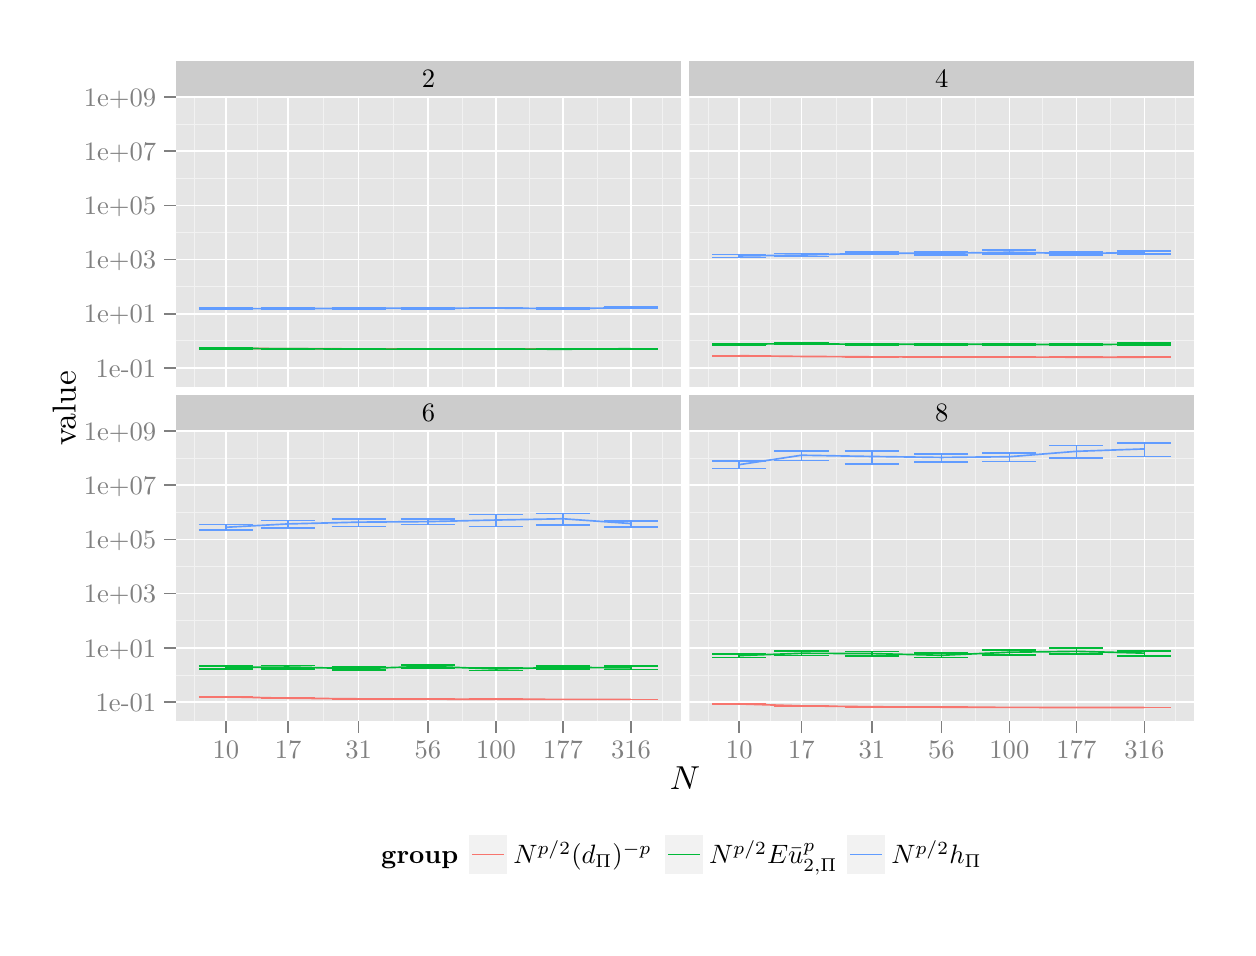
\begin{tikzpicture}[x=1pt,y=1pt]
\definecolor[named]{fillColor}{rgb}{1.00,1.00,1.00}
\path[use as bounding box,fill=fillColor,fill opacity=0.00] (0,0) rectangle (433.62,325.21);
\begin{scope}
\path[clip] (  0.00,  0.00) rectangle (433.62,325.21);
\definecolor[named]{drawColor}{rgb}{1.00,1.00,1.00}
\definecolor[named]{fillColor}{rgb}{1.00,1.00,1.00}

\path[draw=drawColor,line width= 0.6pt,line join=round,line cap=round,fill=fillColor] (  0.00,  0.00) rectangle (433.62,325.21);
\end{scope}
\begin{scope}
\path[clip] ( 53.55,195.47) rectangle (236.06,300.54);
\definecolor[named]{fillColor}{rgb}{0.90,0.90,0.90}

\path[fill=fillColor] ( 53.55,195.47) rectangle (236.06,300.54);
\definecolor[named]{drawColor}{rgb}{0.95,0.95,0.95}

\path[draw=drawColor,line width= 0.3pt,line join=round] ( 53.55,212.02) --
	(236.06,212.02);

\path[draw=drawColor,line width= 0.3pt,line join=round] ( 53.55,231.61) --
	(236.06,231.61);

\path[draw=drawColor,line width= 0.3pt,line join=round] ( 53.55,251.20) --
	(236.06,251.20);

\path[draw=drawColor,line width= 0.3pt,line join=round] ( 53.55,270.80) --
	(236.06,270.80);

\path[draw=drawColor,line width= 0.3pt,line join=round] ( 53.55,290.39) --
	(236.06,290.39);

\path[draw=drawColor,line width= 0.3pt,line join=round] ( 60.36,195.47) --
	( 60.36,300.54);

\path[draw=drawColor,line width= 0.3pt,line join=round] ( 82.85,195.47) --
	( 82.85,300.54);

\path[draw=drawColor,line width= 0.3pt,line join=round] (106.84,195.47) --
	(106.84,300.54);

\path[draw=drawColor,line width= 0.3pt,line join=round] (132.11,195.47) --
	(132.11,300.54);

\path[draw=drawColor,line width= 0.3pt,line join=round] (156.93,195.47) --
	(156.93,300.54);

\path[draw=drawColor,line width= 0.3pt,line join=round] (181.33,195.47) --
	(181.33,300.54);

\path[draw=drawColor,line width= 0.3pt,line join=round] (205.71,195.47) --
	(205.71,300.54);

\path[draw=drawColor,line width= 0.3pt,line join=round] (229.25,195.47) --
	(229.25,300.54);
\definecolor[named]{drawColor}{rgb}{1.00,1.00,1.00}

\path[draw=drawColor,line width= 0.6pt,line join=round] ( 53.55,202.22) --
	(236.06,202.22);

\path[draw=drawColor,line width= 0.6pt,line join=round] ( 53.55,221.81) --
	(236.06,221.81);

\path[draw=drawColor,line width= 0.6pt,line join=round] ( 53.55,241.41) --
	(236.06,241.41);

\path[draw=drawColor,line width= 0.6pt,line join=round] ( 53.55,261.00) --
	(236.06,261.00);

\path[draw=drawColor,line width= 0.6pt,line join=round] ( 53.55,280.59) --
	(236.06,280.59);

\path[draw=drawColor,line width= 0.6pt,line join=round] ( 53.55,300.19) --
	(236.06,300.19);

\path[draw=drawColor,line width= 0.6pt,line join=round] ( 71.61,195.47) --
	( 71.61,300.54);

\path[draw=drawColor,line width= 0.6pt,line join=round] ( 94.10,195.47) --
	( 94.10,300.54);

\path[draw=drawColor,line width= 0.6pt,line join=round] (119.57,195.47) --
	(119.57,300.54);

\path[draw=drawColor,line width= 0.6pt,line join=round] (144.64,195.47) --
	(144.64,300.54);

\path[draw=drawColor,line width= 0.6pt,line join=round] (169.22,195.47) --
	(169.22,300.54);

\path[draw=drawColor,line width= 0.6pt,line join=round] (193.43,195.47) --
	(193.43,300.54);

\path[draw=drawColor,line width= 0.6pt,line join=round] (218.00,195.47) --
	(218.00,300.54);
\definecolor[named]{drawColor}{rgb}{0.97,0.46,0.43}

\path[draw=drawColor,line width= 0.6pt,line join=round] ( 71.61,209.33) --
	( 94.10,209.21) --
	(119.57,209.14) --
	(144.64,209.11) --
	(169.22,209.09) --
	(193.43,209.08) --
	(218.00,209.07);
\definecolor[named]{drawColor}{rgb}{0.00,0.73,0.22}

\path[draw=drawColor,line width= 0.6pt,line join=round] ( 71.61,209.30) --
	( 94.10,209.20) --
	(119.57,209.05) --
	(144.64,209.08) --
	(169.22,209.11) --
	(193.43,209.01) --
	(218.00,209.19);
\definecolor[named]{drawColor}{rgb}{0.38,0.61,1.00}

\path[draw=drawColor,line width= 0.6pt,line join=round] ( 71.61,223.69) --
	( 94.10,223.69) --
	(119.57,223.78) --
	(144.64,223.83) --
	(169.22,223.87) --
	(193.43,223.71) --
	(218.00,224.00);
\definecolor[named]{drawColor}{rgb}{0.97,0.46,0.43}

\path[draw=drawColor,line width= 0.6pt,line join=round] ( 61.85,209.34) --
	( 81.37,209.34);

\path[draw=drawColor,line width= 0.6pt,line join=round] ( 71.61,209.34) --
	( 71.61,209.32);

\path[draw=drawColor,line width= 0.6pt,line join=round] ( 61.85,209.32) --
	( 81.37,209.32);

\path[draw=drawColor,line width= 0.6pt,line join=round] ( 84.34,209.21) --
	(103.86,209.21);

\path[draw=drawColor,line width= 0.6pt,line join=round] ( 94.10,209.21) --
	( 94.10,209.20);

\path[draw=drawColor,line width= 0.6pt,line join=round] ( 84.34,209.20) --
	(103.86,209.20);

\path[draw=drawColor,line width= 0.6pt,line join=round] (109.81,209.14) --
	(129.33,209.14);

\path[draw=drawColor,line width= 0.6pt,line join=round] (119.57,209.14) --
	(119.57,209.14);

\path[draw=drawColor,line width= 0.6pt,line join=round] (109.81,209.14) --
	(129.33,209.14);

\path[draw=drawColor,line width= 0.6pt,line join=round] (134.88,209.11) --
	(154.40,209.11);

\path[draw=drawColor,line width= 0.6pt,line join=round] (144.64,209.11) --
	(144.64,209.11);

\path[draw=drawColor,line width= 0.6pt,line join=round] (134.88,209.11) --
	(154.40,209.11);

\path[draw=drawColor,line width= 0.6pt,line join=round] (159.46,209.09) --
	(178.98,209.09);

\path[draw=drawColor,line width= 0.6pt,line join=round] (169.22,209.09) --
	(169.22,209.09);

\path[draw=drawColor,line width= 0.6pt,line join=round] (159.46,209.09) --
	(178.98,209.09);

\path[draw=drawColor,line width= 0.6pt,line join=round] (183.67,209.08) --
	(203.19,209.08);

\path[draw=drawColor,line width= 0.6pt,line join=round] (193.43,209.08) --
	(193.43,209.08);

\path[draw=drawColor,line width= 0.6pt,line join=round] (183.67,209.08) --
	(203.19,209.08);

\path[draw=drawColor,line width= 0.6pt,line join=round] (208.24,209.07) --
	(227.76,209.07);

\path[draw=drawColor,line width= 0.6pt,line join=round] (218.00,209.07) --
	(218.00,209.07);

\path[draw=drawColor,line width= 0.6pt,line join=round] (208.24,209.07) --
	(227.76,209.07);
\definecolor[named]{drawColor}{rgb}{0.00,0.73,0.22}

\path[draw=drawColor,line width= 0.6pt,line join=round] ( 61.85,209.41) --
	( 81.37,209.41);

\path[draw=drawColor,line width= 0.6pt,line join=round] ( 71.61,209.41) --
	( 71.61,209.19);

\path[draw=drawColor,line width= 0.6pt,line join=round] ( 61.85,209.19) --
	( 81.37,209.19);

\path[draw=drawColor,line width= 0.6pt,line join=round] ( 84.34,209.33) --
	(103.86,209.33);

\path[draw=drawColor,line width= 0.6pt,line join=round] ( 94.10,209.33) --
	( 94.10,209.09);

\path[draw=drawColor,line width= 0.6pt,line join=round] ( 84.34,209.09) --
	(103.86,209.09);

\path[draw=drawColor,line width= 0.6pt,line join=round] (109.81,209.16) --
	(129.33,209.16);

\path[draw=drawColor,line width= 0.6pt,line join=round] (119.57,209.16) --
	(119.57,208.93);

\path[draw=drawColor,line width= 0.6pt,line join=round] (109.81,208.93) --
	(129.33,208.93);

\path[draw=drawColor,line width= 0.6pt,line join=round] (134.88,209.20) --
	(154.40,209.20);

\path[draw=drawColor,line width= 0.6pt,line join=round] (144.64,209.20) --
	(144.64,208.97);

\path[draw=drawColor,line width= 0.6pt,line join=round] (134.88,208.97) --
	(154.40,208.97);

\path[draw=drawColor,line width= 0.6pt,line join=round] (159.46,209.22) --
	(178.98,209.22);

\path[draw=drawColor,line width= 0.6pt,line join=round] (169.22,209.22) --
	(169.22,208.99);

\path[draw=drawColor,line width= 0.6pt,line join=round] (159.46,208.99) --
	(178.98,208.99);

\path[draw=drawColor,line width= 0.6pt,line join=round] (183.67,209.13) --
	(203.19,209.13);

\path[draw=drawColor,line width= 0.6pt,line join=round] (193.43,209.13) --
	(193.43,208.90);

\path[draw=drawColor,line width= 0.6pt,line join=round] (183.67,208.90) --
	(203.19,208.90);

\path[draw=drawColor,line width= 0.6pt,line join=round] (208.24,209.31) --
	(227.76,209.31);

\path[draw=drawColor,line width= 0.6pt,line join=round] (218.00,209.31) --
	(218.00,209.07);

\path[draw=drawColor,line width= 0.6pt,line join=round] (208.24,209.07) --
	(227.76,209.07);
\definecolor[named]{drawColor}{rgb}{0.38,0.61,1.00}

\path[draw=drawColor,line width= 0.6pt,line join=round] ( 61.85,223.87) --
	( 81.37,223.87);

\path[draw=drawColor,line width= 0.6pt,line join=round] ( 71.61,223.87) --
	( 71.61,223.51);

\path[draw=drawColor,line width= 0.6pt,line join=round] ( 61.85,223.51) --
	( 81.37,223.51);

\path[draw=drawColor,line width= 0.6pt,line join=round] ( 84.34,223.88) --
	(103.86,223.88);

\path[draw=drawColor,line width= 0.6pt,line join=round] ( 94.10,223.88) --
	( 94.10,223.49);

\path[draw=drawColor,line width= 0.6pt,line join=round] ( 84.34,223.49) --
	(103.86,223.49);

\path[draw=drawColor,line width= 0.6pt,line join=round] (109.81,223.99) --
	(129.33,223.99);

\path[draw=drawColor,line width= 0.6pt,line join=round] (119.57,223.99) --
	(119.57,223.57);

\path[draw=drawColor,line width= 0.6pt,line join=round] (109.81,223.57) --
	(129.33,223.57);

\path[draw=drawColor,line width= 0.6pt,line join=round] (134.88,224.04) --
	(154.40,224.04);

\path[draw=drawColor,line width= 0.6pt,line join=round] (144.64,224.04) --
	(144.64,223.64);

\path[draw=drawColor,line width= 0.6pt,line join=round] (134.88,223.64) --
	(154.40,223.64);

\path[draw=drawColor,line width= 0.6pt,line join=round] (159.46,224.07) --
	(178.98,224.07);

\path[draw=drawColor,line width= 0.6pt,line join=round] (169.22,224.07) --
	(169.22,223.69);

\path[draw=drawColor,line width= 0.6pt,line join=round] (159.46,223.69) --
	(178.98,223.69);

\path[draw=drawColor,line width= 0.6pt,line join=round] (183.67,223.92) --
	(203.19,223.92);

\path[draw=drawColor,line width= 0.6pt,line join=round] (193.43,223.92) --
	(193.43,223.49);

\path[draw=drawColor,line width= 0.6pt,line join=round] (183.67,223.49) --
	(203.19,223.49);

\path[draw=drawColor,line width= 0.6pt,line join=round] (208.24,224.21) --
	(227.76,224.21);

\path[draw=drawColor,line width= 0.6pt,line join=round] (218.00,224.21) --
	(218.00,223.79);

\path[draw=drawColor,line width= 0.6pt,line join=round] (208.24,223.79) --
	(227.76,223.79);
\end{scope}
\begin{scope}
\path[clip] (239.07,195.47) rectangle (421.58,300.54);
\definecolor[named]{fillColor}{rgb}{0.90,0.90,0.90}

\path[fill=fillColor] (239.07,195.47) rectangle (421.57,300.54);
\definecolor[named]{drawColor}{rgb}{0.95,0.95,0.95}

\path[draw=drawColor,line width= 0.3pt,line join=round] (239.07,212.02) --
	(421.58,212.02);

\path[draw=drawColor,line width= 0.3pt,line join=round] (239.07,231.61) --
	(421.58,231.61);

\path[draw=drawColor,line width= 0.3pt,line join=round] (239.07,251.20) --
	(421.58,251.20);

\path[draw=drawColor,line width= 0.3pt,line join=round] (239.07,270.80) --
	(421.58,270.80);

\path[draw=drawColor,line width= 0.3pt,line join=round] (239.07,290.39) --
	(421.58,290.39);

\path[draw=drawColor,line width= 0.3pt,line join=round] (245.88,195.47) --
	(245.88,300.54);

\path[draw=drawColor,line width= 0.3pt,line join=round] (268.37,195.47) --
	(268.37,300.54);

\path[draw=drawColor,line width= 0.3pt,line join=round] (292.36,195.47) --
	(292.36,300.54);

\path[draw=drawColor,line width= 0.3pt,line join=round] (317.62,195.47) --
	(317.62,300.54);

\path[draw=drawColor,line width= 0.3pt,line join=round] (342.45,195.47) --
	(342.45,300.54);

\path[draw=drawColor,line width= 0.3pt,line join=round] (366.84,195.47) --
	(366.84,300.54);

\path[draw=drawColor,line width= 0.3pt,line join=round] (391.23,195.47) --
	(391.23,300.54);

\path[draw=drawColor,line width= 0.3pt,line join=round] (414.77,195.47) --
	(414.77,300.54);
\definecolor[named]{drawColor}{rgb}{1.00,1.00,1.00}

\path[draw=drawColor,line width= 0.6pt,line join=round] (239.07,202.22) --
	(421.58,202.22);

\path[draw=drawColor,line width= 0.6pt,line join=round] (239.07,221.81) --
	(421.58,221.81);

\path[draw=drawColor,line width= 0.6pt,line join=round] (239.07,241.41) --
	(421.58,241.41);

\path[draw=drawColor,line width= 0.6pt,line join=round] (239.07,261.00) --
	(421.58,261.00);

\path[draw=drawColor,line width= 0.6pt,line join=round] (239.07,280.59) --
	(421.58,280.59);

\path[draw=drawColor,line width= 0.6pt,line join=round] (239.07,300.19) --
	(421.58,300.19);

\path[draw=drawColor,line width= 0.6pt,line join=round] (257.13,195.47) --
	(257.13,300.54);

\path[draw=drawColor,line width= 0.6pt,line join=round] (279.62,195.47) --
	(279.62,300.54);

\path[draw=drawColor,line width= 0.6pt,line join=round] (305.09,195.47) --
	(305.09,300.54);

\path[draw=drawColor,line width= 0.6pt,line join=round] (330.16,195.47) --
	(330.16,300.54);

\path[draw=drawColor,line width= 0.6pt,line join=round] (354.74,195.47) --
	(354.74,300.54);

\path[draw=drawColor,line width= 0.6pt,line join=round] (378.95,195.47) --
	(378.95,300.54);

\path[draw=drawColor,line width= 0.6pt,line join=round] (403.52,195.47) --
	(403.52,300.54);
\definecolor[named]{drawColor}{rgb}{0.97,0.46,0.43}

\path[draw=drawColor,line width= 0.6pt,line join=round] (257.13,206.67) --
	(279.62,206.41) --
	(305.09,206.26) --
	(330.16,206.20) --
	(354.74,206.16) --
	(378.95,206.14) --
	(403.52,206.13);
\definecolor[named]{drawColor}{rgb}{0.00,0.73,0.22}

\path[draw=drawColor,line width= 0.6pt,line join=round] (257.13,210.90) --
	(279.62,210.97) --
	(305.09,210.79) --
	(330.16,210.82) --
	(354.74,210.83) --
	(378.95,210.61) --
	(403.52,210.88);
\definecolor[named]{drawColor}{rgb}{0.38,0.61,1.00}

\path[draw=drawColor,line width= 0.6pt,line join=round] (257.13,242.71) --
	(279.62,243.03) --
	(305.09,243.70) --
	(330.16,243.68) --
	(354.74,244.06) --
	(378.95,243.59) --
	(403.52,243.97);
\definecolor[named]{drawColor}{rgb}{0.97,0.46,0.43}

\path[draw=drawColor,line width= 0.6pt,line join=round] (247.36,206.69) --
	(266.89,206.69);

\path[draw=drawColor,line width= 0.6pt,line join=round] (257.13,206.69) --
	(257.13,206.65);

\path[draw=drawColor,line width= 0.6pt,line join=round] (247.36,206.65) --
	(266.89,206.65);

\path[draw=drawColor,line width= 0.6pt,line join=round] (269.86,206.42) --
	(289.38,206.42);

\path[draw=drawColor,line width= 0.6pt,line join=round] (279.62,206.42) --
	(279.62,206.40);

\path[draw=drawColor,line width= 0.6pt,line join=round] (269.86,206.40) --
	(289.38,206.40);

\path[draw=drawColor,line width= 0.6pt,line join=round] (295.33,206.27) --
	(314.85,206.27);

\path[draw=drawColor,line width= 0.6pt,line join=round] (305.09,206.27) --
	(305.09,206.26);

\path[draw=drawColor,line width= 0.6pt,line join=round] (295.33,206.26) --
	(314.85,206.26);

\path[draw=drawColor,line width= 0.6pt,line join=round] (320.40,206.20) --
	(339.92,206.20);

\path[draw=drawColor,line width= 0.6pt,line join=round] (330.16,206.20) --
	(330.16,206.20);

\path[draw=drawColor,line width= 0.6pt,line join=round] (320.40,206.20) --
	(339.92,206.20);

\path[draw=drawColor,line width= 0.6pt,line join=round] (344.98,206.16) --
	(364.50,206.16);

\path[draw=drawColor,line width= 0.6pt,line join=round] (354.74,206.16) --
	(354.74,206.16);

\path[draw=drawColor,line width= 0.6pt,line join=round] (344.98,206.16) --
	(364.50,206.16);

\path[draw=drawColor,line width= 0.6pt,line join=round] (369.19,206.14) --
	(388.71,206.14);

\path[draw=drawColor,line width= 0.6pt,line join=round] (378.95,206.14) --
	(378.95,206.14);

\path[draw=drawColor,line width= 0.6pt,line join=round] (369.19,206.14) --
	(388.71,206.14);

\path[draw=drawColor,line width= 0.6pt,line join=round] (393.76,206.13) --
	(413.28,206.13);

\path[draw=drawColor,line width= 0.6pt,line join=round] (403.52,206.13) --
	(403.52,206.13);

\path[draw=drawColor,line width= 0.6pt,line join=round] (393.76,206.13) --
	(413.28,206.13);
\definecolor[named]{drawColor}{rgb}{0.00,0.73,0.22}

\path[draw=drawColor,line width= 0.6pt,line join=round] (247.36,211.12) --
	(266.89,211.12);

\path[draw=drawColor,line width= 0.6pt,line join=round] (257.13,211.12) --
	(257.13,210.66);

\path[draw=drawColor,line width= 0.6pt,line join=round] (247.36,210.66) --
	(266.89,210.66);

\path[draw=drawColor,line width= 0.6pt,line join=round] (269.86,211.21) --
	(289.38,211.21);

\path[draw=drawColor,line width= 0.6pt,line join=round] (279.62,211.21) --
	(279.62,210.70);

\path[draw=drawColor,line width= 0.6pt,line join=round] (269.86,210.70) --
	(289.38,210.70);

\path[draw=drawColor,line width= 0.6pt,line join=round] (295.33,211.04) --
	(314.85,211.04);

\path[draw=drawColor,line width= 0.6pt,line join=round] (305.09,211.04) --
	(305.09,210.51);

\path[draw=drawColor,line width= 0.6pt,line join=round] (295.33,210.51) --
	(314.85,210.51);

\path[draw=drawColor,line width= 0.6pt,line join=round] (320.40,211.08) --
	(339.92,211.08);

\path[draw=drawColor,line width= 0.6pt,line join=round] (330.16,211.08) --
	(330.16,210.57);

\path[draw=drawColor,line width= 0.6pt,line join=round] (320.40,210.57) --
	(339.92,210.57);

\path[draw=drawColor,line width= 0.6pt,line join=round] (344.98,211.09) --
	(364.50,211.09);

\path[draw=drawColor,line width= 0.6pt,line join=round] (354.74,211.09) --
	(354.74,210.57);

\path[draw=drawColor,line width= 0.6pt,line join=round] (344.98,210.57) --
	(364.50,210.57);

\path[draw=drawColor,line width= 0.6pt,line join=round] (369.19,210.89) --
	(388.71,210.89);

\path[draw=drawColor,line width= 0.6pt,line join=round] (378.95,210.89) --
	(378.95,210.32);

\path[draw=drawColor,line width= 0.6pt,line join=round] (369.19,210.32) --
	(388.71,210.32);

\path[draw=drawColor,line width= 0.6pt,line join=round] (393.76,211.15) --
	(413.28,211.15);

\path[draw=drawColor,line width= 0.6pt,line join=round] (403.52,211.15) --
	(403.52,210.62);

\path[draw=drawColor,line width= 0.6pt,line join=round] (393.76,210.62) --
	(413.28,210.62);
\definecolor[named]{drawColor}{rgb}{0.38,0.61,1.00}

\path[draw=drawColor,line width= 0.6pt,line join=round] (247.36,243.21) --
	(266.89,243.21);

\path[draw=drawColor,line width= 0.6pt,line join=round] (257.13,243.21) --
	(257.13,242.20);

\path[draw=drawColor,line width= 0.6pt,line join=round] (247.36,242.20) --
	(266.89,242.20);

\path[draw=drawColor,line width= 0.6pt,line join=round] (269.86,243.60) --
	(289.38,243.60);

\path[draw=drawColor,line width= 0.6pt,line join=round] (279.62,243.60) --
	(279.62,242.48);

\path[draw=drawColor,line width= 0.6pt,line join=round] (269.86,242.48) --
	(289.38,242.48);

\path[draw=drawColor,line width= 0.6pt,line join=round] (295.33,244.20) --
	(314.85,244.20);

\path[draw=drawColor,line width= 0.6pt,line join=round] (305.09,244.20) --
	(305.09,243.20);

\path[draw=drawColor,line width= 0.6pt,line join=round] (295.33,243.20) --
	(314.85,243.20);

\path[draw=drawColor,line width= 0.6pt,line join=round] (320.40,244.26) --
	(339.92,244.26);

\path[draw=drawColor,line width= 0.6pt,line join=round] (330.16,244.26) --
	(330.16,243.09);

\path[draw=drawColor,line width= 0.6pt,line join=round] (320.40,243.09) --
	(339.92,243.09);

\path[draw=drawColor,line width= 0.6pt,line join=round] (344.98,244.82) --
	(364.50,244.82);

\path[draw=drawColor,line width= 0.6pt,line join=round] (354.74,244.82) --
	(354.74,243.34);

\path[draw=drawColor,line width= 0.6pt,line join=round] (344.98,243.34) --
	(364.50,243.34);

\path[draw=drawColor,line width= 0.6pt,line join=round] (369.19,244.12) --
	(388.71,244.12);

\path[draw=drawColor,line width= 0.6pt,line join=round] (378.95,244.12) --
	(378.95,243.04);

\path[draw=drawColor,line width= 0.6pt,line join=round] (369.19,243.04) --
	(388.71,243.04);

\path[draw=drawColor,line width= 0.6pt,line join=round] (393.76,244.58) --
	(413.28,244.58);

\path[draw=drawColor,line width= 0.6pt,line join=round] (403.52,244.58) --
	(403.52,243.33);

\path[draw=drawColor,line width= 0.6pt,line join=round] (393.76,243.33) --
	(413.28,243.33);
\end{scope}
\begin{scope}
\path[clip] ( 53.55, 74.76) rectangle (236.06,179.83);
\definecolor[named]{fillColor}{rgb}{0.90,0.90,0.90}

\path[fill=fillColor] ( 53.55, 74.76) rectangle (236.06,179.83);
\definecolor[named]{drawColor}{rgb}{0.95,0.95,0.95}

\path[draw=drawColor,line width= 0.3pt,line join=round] ( 53.55, 91.31) --
	(236.06, 91.31);

\path[draw=drawColor,line width= 0.3pt,line join=round] ( 53.55,110.90) --
	(236.06,110.90);

\path[draw=drawColor,line width= 0.3pt,line join=round] ( 53.55,130.49) --
	(236.06,130.49);

\path[draw=drawColor,line width= 0.3pt,line join=round] ( 53.55,150.09) --
	(236.06,150.09);

\path[draw=drawColor,line width= 0.3pt,line join=round] ( 53.55,169.68) --
	(236.06,169.68);

\path[draw=drawColor,line width= 0.3pt,line join=round] ( 60.36, 74.76) --
	( 60.36,179.83);

\path[draw=drawColor,line width= 0.3pt,line join=round] ( 82.85, 74.76) --
	( 82.85,179.83);

\path[draw=drawColor,line width= 0.3pt,line join=round] (106.84, 74.76) --
	(106.84,179.83);

\path[draw=drawColor,line width= 0.3pt,line join=round] (132.11, 74.76) --
	(132.11,179.83);

\path[draw=drawColor,line width= 0.3pt,line join=round] (156.93, 74.76) --
	(156.93,179.83);

\path[draw=drawColor,line width= 0.3pt,line join=round] (181.33, 74.76) --
	(181.33,179.83);

\path[draw=drawColor,line width= 0.3pt,line join=round] (205.71, 74.76) --
	(205.71,179.83);

\path[draw=drawColor,line width= 0.3pt,line join=round] (229.25, 74.76) --
	(229.25,179.83);
\definecolor[named]{drawColor}{rgb}{1.00,1.00,1.00}

\path[draw=drawColor,line width= 0.6pt,line join=round] ( 53.55, 81.51) --
	(236.06, 81.51);

\path[draw=drawColor,line width= 0.6pt,line join=round] ( 53.55,101.10) --
	(236.06,101.10);

\path[draw=drawColor,line width= 0.6pt,line join=round] ( 53.55,120.70) --
	(236.06,120.70);

\path[draw=drawColor,line width= 0.6pt,line join=round] ( 53.55,140.29) --
	(236.06,140.29);

\path[draw=drawColor,line width= 0.6pt,line join=round] ( 53.55,159.88) --
	(236.06,159.88);

\path[draw=drawColor,line width= 0.6pt,line join=round] ( 53.55,179.48) --
	(236.06,179.48);

\path[draw=drawColor,line width= 0.6pt,line join=round] ( 71.61, 74.76) --
	( 71.61,179.83);

\path[draw=drawColor,line width= 0.6pt,line join=round] ( 94.10, 74.76) --
	( 94.10,179.83);

\path[draw=drawColor,line width= 0.6pt,line join=round] (119.57, 74.76) --
	(119.57,179.83);

\path[draw=drawColor,line width= 0.6pt,line join=round] (144.64, 74.76) --
	(144.64,179.83);

\path[draw=drawColor,line width= 0.6pt,line join=round] (169.22, 74.76) --
	(169.22,179.83);

\path[draw=drawColor,line width= 0.6pt,line join=round] (193.43, 74.76) --
	(193.43,179.83);

\path[draw=drawColor,line width= 0.6pt,line join=round] (218.00, 74.76) --
	(218.00,179.83);
\definecolor[named]{drawColor}{rgb}{0.97,0.46,0.43}

\path[draw=drawColor,line width= 0.6pt,line join=round] ( 71.61, 83.41) --
	( 94.10, 82.91) --
	(119.57, 82.68) --
	(144.64, 82.58) --
	(169.22, 82.52) --
	(193.43, 82.50) --
	(218.00, 82.48);
\definecolor[named]{drawColor}{rgb}{0.00,0.73,0.22}

\path[draw=drawColor,line width= 0.6pt,line join=round] ( 71.61, 94.00) --
	( 94.10, 94.17) --
	(119.57, 93.60) --
	(144.64, 94.41) --
	(169.22, 93.48) --
	(193.43, 94.05) --
	(218.00, 93.88);
\definecolor[named]{drawColor}{rgb}{0.38,0.61,1.00}

\path[draw=drawColor,line width= 0.6pt,line join=round] ( 71.61,144.68) --
	( 94.10,145.89) --
	(119.57,146.53) --
	(144.64,146.73) --
	(169.22,147.29) --
	(193.43,147.75) --
	(218.00,146.02);
\definecolor[named]{drawColor}{rgb}{0.97,0.46,0.43}

\path[draw=drawColor,line width= 0.6pt,line join=round] ( 61.85, 83.46) --
	( 81.37, 83.46);

\path[draw=drawColor,line width= 0.6pt,line join=round] ( 71.61, 83.46) --
	( 71.61, 83.36);

\path[draw=drawColor,line width= 0.6pt,line join=round] ( 61.85, 83.36) --
	( 81.37, 83.36);

\path[draw=drawColor,line width= 0.6pt,line join=round] ( 84.34, 82.93) --
	(103.86, 82.93);

\path[draw=drawColor,line width= 0.6pt,line join=round] ( 94.10, 82.93) --
	( 94.10, 82.89);

\path[draw=drawColor,line width= 0.6pt,line join=round] ( 84.34, 82.89) --
	(103.86, 82.89);

\path[draw=drawColor,line width= 0.6pt,line join=round] (109.81, 82.69) --
	(129.33, 82.69);

\path[draw=drawColor,line width= 0.6pt,line join=round] (119.57, 82.69) --
	(119.57, 82.68);

\path[draw=drawColor,line width= 0.6pt,line join=round] (109.81, 82.68) --
	(129.33, 82.68);

\path[draw=drawColor,line width= 0.6pt,line join=round] (134.88, 82.59) --
	(154.40, 82.59);

\path[draw=drawColor,line width= 0.6pt,line join=round] (144.64, 82.59) --
	(144.64, 82.58);

\path[draw=drawColor,line width= 0.6pt,line join=round] (134.88, 82.58) --
	(154.40, 82.58);

\path[draw=drawColor,line width= 0.6pt,line join=round] (159.46, 82.52) --
	(178.98, 82.52);

\path[draw=drawColor,line width= 0.6pt,line join=round] (169.22, 82.52) --
	(169.22, 82.52);

\path[draw=drawColor,line width= 0.6pt,line join=round] (159.46, 82.52) --
	(178.98, 82.52);

\path[draw=drawColor,line width= 0.6pt,line join=round] (183.67, 82.50) --
	(203.19, 82.50);

\path[draw=drawColor,line width= 0.6pt,line join=round] (193.43, 82.50) --
	(193.43, 82.49);

\path[draw=drawColor,line width= 0.6pt,line join=round] (183.67, 82.49) --
	(203.19, 82.49);

\path[draw=drawColor,line width= 0.6pt,line join=round] (208.24, 82.48) --
	(227.76, 82.48);

\path[draw=drawColor,line width= 0.6pt,line join=round] (218.00, 82.48) --
	(218.00, 82.48);

\path[draw=drawColor,line width= 0.6pt,line join=round] (208.24, 82.48) --
	(227.76, 82.48);
\definecolor[named]{drawColor}{rgb}{0.00,0.73,0.22}

\path[draw=drawColor,line width= 0.6pt,line join=round] ( 61.85, 94.43) --
	( 81.37, 94.43);

\path[draw=drawColor,line width= 0.6pt,line join=round] ( 71.61, 94.43) --
	( 71.61, 93.57);

\path[draw=drawColor,line width= 0.6pt,line join=round] ( 61.85, 93.57) --
	( 81.37, 93.57);

\path[draw=drawColor,line width= 0.6pt,line join=round] ( 84.34, 94.79) --
	(103.86, 94.79);

\path[draw=drawColor,line width= 0.6pt,line join=round] ( 94.10, 94.79) --
	( 94.10, 93.52);

\path[draw=drawColor,line width= 0.6pt,line join=round] ( 84.34, 93.52) --
	(103.86, 93.52);

\path[draw=drawColor,line width= 0.6pt,line join=round] (109.81, 94.14) --
	(129.33, 94.14);

\path[draw=drawColor,line width= 0.6pt,line join=round] (119.57, 94.14) --
	(119.57, 93.13);

\path[draw=drawColor,line width= 0.6pt,line join=round] (109.81, 93.13) --
	(129.33, 93.13);

\path[draw=drawColor,line width= 0.6pt,line join=round] (134.88, 94.91) --
	(154.40, 94.91);

\path[draw=drawColor,line width= 0.6pt,line join=round] (144.64, 94.91) --
	(144.64, 93.89);

\path[draw=drawColor,line width= 0.6pt,line join=round] (134.88, 93.89) --
	(154.40, 93.89);

\path[draw=drawColor,line width= 0.6pt,line join=round] (159.46, 94.01) --
	(178.98, 94.01);

\path[draw=drawColor,line width= 0.6pt,line join=round] (169.22, 94.01) --
	(169.22, 92.93);

\path[draw=drawColor,line width= 0.6pt,line join=round] (159.46, 92.93) --
	(178.98, 92.93);

\path[draw=drawColor,line width= 0.6pt,line join=round] (183.67, 94.56) --
	(203.19, 94.56);

\path[draw=drawColor,line width= 0.6pt,line join=round] (193.43, 94.56) --
	(193.43, 93.54);

\path[draw=drawColor,line width= 0.6pt,line join=round] (183.67, 93.54) --
	(203.19, 93.54);

\path[draw=drawColor,line width= 0.6pt,line join=round] (208.24, 94.45) --
	(227.76, 94.45);

\path[draw=drawColor,line width= 0.6pt,line join=round] (218.00, 94.45) --
	(218.00, 93.31);

\path[draw=drawColor,line width= 0.6pt,line join=round] (208.24, 93.31) --
	(227.76, 93.31);
\definecolor[named]{drawColor}{rgb}{0.38,0.61,1.00}

\path[draw=drawColor,line width= 0.6pt,line join=round] ( 61.85,145.62) --
	( 81.37,145.62);

\path[draw=drawColor,line width= 0.6pt,line join=round] ( 71.61,145.62) --
	( 71.61,143.63);

\path[draw=drawColor,line width= 0.6pt,line join=round] ( 61.85,143.63) --
	( 81.37,143.63);

\path[draw=drawColor,line width= 0.6pt,line join=round] ( 84.34,147.14) --
	(103.86,147.14);

\path[draw=drawColor,line width= 0.6pt,line join=round] ( 94.10,147.14) --
	( 94.10,144.47);

\path[draw=drawColor,line width= 0.6pt,line join=round] ( 84.34,144.47) --
	(103.86,144.47);

\path[draw=drawColor,line width= 0.6pt,line join=round] (109.81,147.78) --
	(129.33,147.78);

\path[draw=drawColor,line width= 0.6pt,line join=round] (119.57,147.78) --
	(119.57,145.00);

\path[draw=drawColor,line width= 0.6pt,line join=round] (109.81,145.00) --
	(129.33,145.00);

\path[draw=drawColor,line width= 0.6pt,line join=round] (134.88,147.72) --
	(154.40,147.72);

\path[draw=drawColor,line width= 0.6pt,line join=round] (144.64,147.72) --
	(144.64,145.67);

\path[draw=drawColor,line width= 0.6pt,line join=round] (134.88,145.67) --
	(154.40,145.67);

\path[draw=drawColor,line width= 0.6pt,line join=round] (159.46,149.25) --
	(178.98,149.25);

\path[draw=drawColor,line width= 0.6pt,line join=round] (169.22,149.25) --
	(169.22,144.93);

\path[draw=drawColor,line width= 0.6pt,line join=round] (159.46,144.93) --
	(178.98,144.93);

\path[draw=drawColor,line width= 0.6pt,line join=round] (183.67,149.67) --
	(203.19,149.67);

\path[draw=drawColor,line width= 0.6pt,line join=round] (193.43,149.67) --
	(193.43,145.41);

\path[draw=drawColor,line width= 0.6pt,line join=round] (183.67,145.41) --
	(203.19,145.41);

\path[draw=drawColor,line width= 0.6pt,line join=round] (208.24,147.04) --
	(227.76,147.04);

\path[draw=drawColor,line width= 0.6pt,line join=round] (218.00,147.04) --
	(218.00,144.76);

\path[draw=drawColor,line width= 0.6pt,line join=round] (208.24,144.76) --
	(227.76,144.76);
\end{scope}
\begin{scope}
\path[clip] (239.07, 74.76) rectangle (421.58,179.83);
\definecolor[named]{fillColor}{rgb}{0.90,0.90,0.90}

\path[fill=fillColor] (239.07, 74.76) rectangle (421.57,179.83);
\definecolor[named]{drawColor}{rgb}{0.95,0.95,0.95}

\path[draw=drawColor,line width= 0.3pt,line join=round] (239.07, 91.31) --
	(421.58, 91.31);

\path[draw=drawColor,line width= 0.3pt,line join=round] (239.07,110.90) --
	(421.58,110.90);

\path[draw=drawColor,line width= 0.3pt,line join=round] (239.07,130.49) --
	(421.58,130.49);

\path[draw=drawColor,line width= 0.3pt,line join=round] (239.07,150.09) --
	(421.58,150.09);

\path[draw=drawColor,line width= 0.3pt,line join=round] (239.07,169.68) --
	(421.58,169.68);

\path[draw=drawColor,line width= 0.3pt,line join=round] (245.88, 74.76) --
	(245.88,179.83);

\path[draw=drawColor,line width= 0.3pt,line join=round] (268.37, 74.76) --
	(268.37,179.83);

\path[draw=drawColor,line width= 0.3pt,line join=round] (292.36, 74.76) --
	(292.36,179.83);

\path[draw=drawColor,line width= 0.3pt,line join=round] (317.62, 74.76) --
	(317.62,179.83);

\path[draw=drawColor,line width= 0.3pt,line join=round] (342.45, 74.76) --
	(342.45,179.83);

\path[draw=drawColor,line width= 0.3pt,line join=round] (366.84, 74.76) --
	(366.84,179.83);

\path[draw=drawColor,line width= 0.3pt,line join=round] (391.23, 74.76) --
	(391.23,179.83);

\path[draw=drawColor,line width= 0.3pt,line join=round] (414.77, 74.76) --
	(414.77,179.83);
\definecolor[named]{drawColor}{rgb}{1.00,1.00,1.00}

\path[draw=drawColor,line width= 0.6pt,line join=round] (239.07, 81.51) --
	(421.58, 81.51);

\path[draw=drawColor,line width= 0.6pt,line join=round] (239.07,101.10) --
	(421.58,101.10);

\path[draw=drawColor,line width= 0.6pt,line join=round] (239.07,120.70) --
	(421.58,120.70);

\path[draw=drawColor,line width= 0.6pt,line join=round] (239.07,140.29) --
	(421.58,140.29);

\path[draw=drawColor,line width= 0.6pt,line join=round] (239.07,159.88) --
	(421.58,159.88);

\path[draw=drawColor,line width= 0.6pt,line join=round] (239.07,179.48) --
	(421.58,179.48);

\path[draw=drawColor,line width= 0.6pt,line join=round] (257.13, 74.76) --
	(257.13,179.83);

\path[draw=drawColor,line width= 0.6pt,line join=round] (279.62, 74.76) --
	(279.62,179.83);

\path[draw=drawColor,line width= 0.6pt,line join=round] (305.09, 74.76) --
	(305.09,179.83);

\path[draw=drawColor,line width= 0.6pt,line join=round] (330.16, 74.76) --
	(330.16,179.83);

\path[draw=drawColor,line width= 0.6pt,line join=round] (354.74, 74.76) --
	(354.74,179.83);

\path[draw=drawColor,line width= 0.6pt,line join=round] (378.95, 74.76) --
	(378.95,179.83);

\path[draw=drawColor,line width= 0.6pt,line join=round] (403.52, 74.76) --
	(403.52,179.83);
\definecolor[named]{drawColor}{rgb}{0.97,0.46,0.43}

\path[draw=drawColor,line width= 0.6pt,line join=round] (257.13, 80.83) --
	(279.62, 80.14) --
	(305.09, 79.82) --
	(330.16, 79.67) --
	(354.74, 79.60) --
	(378.95, 79.56) --
	(403.52, 79.54);
\definecolor[named]{drawColor}{rgb}{0.00,0.73,0.22}

\path[draw=drawColor,line width= 0.6pt,line join=round] (257.13, 98.31) --
	(279.62, 99.14) --
	(305.09, 99.04) --
	(330.16, 98.42) --
	(354.74, 99.53) --
	(378.95, 99.85) --
	(403.52, 99.19);
\definecolor[named]{drawColor}{rgb}{0.38,0.61,1.00}

\path[draw=drawColor,line width= 0.6pt,line join=round] (257.13,167.31) --
	(279.62,170.71) --
	(305.09,170.26) --
	(330.16,169.91) --
	(354.74,170.17) --
	(378.95,172.12) --
	(403.52,172.99);
\definecolor[named]{drawColor}{rgb}{0.97,0.46,0.43}

\path[draw=drawColor,line width= 0.6pt,line join=round] (247.36, 80.89) --
	(266.89, 80.89);

\path[draw=drawColor,line width= 0.6pt,line join=round] (257.13, 80.89) --
	(257.13, 80.77);

\path[draw=drawColor,line width= 0.6pt,line join=round] (247.36, 80.77) --
	(266.89, 80.77);

\path[draw=drawColor,line width= 0.6pt,line join=round] (269.86, 80.17) --
	(289.38, 80.17);

\path[draw=drawColor,line width= 0.6pt,line join=round] (279.62, 80.17) --
	(279.62, 80.12);

\path[draw=drawColor,line width= 0.6pt,line join=round] (269.86, 80.12) --
	(289.38, 80.12);

\path[draw=drawColor,line width= 0.6pt,line join=round] (295.33, 79.83) --
	(314.85, 79.83);

\path[draw=drawColor,line width= 0.6pt,line join=round] (305.09, 79.83) --
	(305.09, 79.81);

\path[draw=drawColor,line width= 0.6pt,line join=round] (295.33, 79.81) --
	(314.85, 79.81);

\path[draw=drawColor,line width= 0.6pt,line join=round] (320.40, 79.67) --
	(339.92, 79.67);

\path[draw=drawColor,line width= 0.6pt,line join=round] (330.16, 79.67) --
	(330.16, 79.66);

\path[draw=drawColor,line width= 0.6pt,line join=round] (320.40, 79.66) --
	(339.92, 79.66);

\path[draw=drawColor,line width= 0.6pt,line join=round] (344.98, 79.60) --
	(364.50, 79.60);

\path[draw=drawColor,line width= 0.6pt,line join=round] (354.74, 79.60) --
	(354.74, 79.60);

\path[draw=drawColor,line width= 0.6pt,line join=round] (344.98, 79.60) --
	(364.50, 79.60);

\path[draw=drawColor,line width= 0.6pt,line join=round] (369.19, 79.56) --
	(388.71, 79.56);

\path[draw=drawColor,line width= 0.6pt,line join=round] (378.95, 79.56) --
	(378.95, 79.56);

\path[draw=drawColor,line width= 0.6pt,line join=round] (369.19, 79.56) --
	(388.71, 79.56);

\path[draw=drawColor,line width= 0.6pt,line join=round] (393.76, 79.54) --
	(413.28, 79.54);

\path[draw=drawColor,line width= 0.6pt,line join=round] (403.52, 79.54) --
	(403.52, 79.54);

\path[draw=drawColor,line width= 0.6pt,line join=round] (393.76, 79.54) --
	(413.28, 79.54);
\definecolor[named]{drawColor}{rgb}{0.00,0.73,0.22}

\path[draw=drawColor,line width= 0.6pt,line join=round] (247.36, 98.86) --
	(266.89, 98.86);

\path[draw=drawColor,line width= 0.6pt,line join=round] (257.13, 98.86) --
	(257.13, 97.68);

\path[draw=drawColor,line width= 0.6pt,line join=round] (247.36, 97.68) --
	(266.89, 97.68);

\path[draw=drawColor,line width= 0.6pt,line join=round] (269.86, 99.86) --
	(289.38, 99.86);

\path[draw=drawColor,line width= 0.6pt,line join=round] (279.62, 99.86) --
	(279.62, 98.34);

\path[draw=drawColor,line width= 0.6pt,line join=round] (269.86, 98.34) --
	(289.38, 98.34);

\path[draw=drawColor,line width= 0.6pt,line join=round] (295.33, 99.79) --
	(314.85, 99.79);

\path[draw=drawColor,line width= 0.6pt,line join=round] (305.09, 99.79) --
	(305.09, 98.23);

\path[draw=drawColor,line width= 0.6pt,line join=round] (295.33, 98.23) --
	(314.85, 98.23);

\path[draw=drawColor,line width= 0.6pt,line join=round] (320.40, 99.24) --
	(339.92, 99.24);

\path[draw=drawColor,line width= 0.6pt,line join=round] (330.16, 99.24) --
	(330.16, 97.63);

\path[draw=drawColor,line width= 0.6pt,line join=round] (320.40, 97.63) --
	(339.92, 97.63);

\path[draw=drawColor,line width= 0.6pt,line join=round] (344.98,100.40) --
	(364.50,100.40);

\path[draw=drawColor,line width= 0.6pt,line join=round] (354.74,100.40) --
	(354.74, 98.55);

\path[draw=drawColor,line width= 0.6pt,line join=round] (344.98, 98.55) --
	(364.50, 98.55);

\path[draw=drawColor,line width= 0.6pt,line join=round] (369.19,100.96) --
	(388.71,100.96);

\path[draw=drawColor,line width= 0.6pt,line join=round] (378.95,100.96) --
	(378.95, 98.78);

\path[draw=drawColor,line width= 0.6pt,line join=round] (369.19, 98.78) --
	(388.71, 98.78);

\path[draw=drawColor,line width= 0.6pt,line join=round] (393.76,100.04) --
	(413.28,100.04);

\path[draw=drawColor,line width= 0.6pt,line join=round] (403.52,100.04) --
	(403.52, 98.28);

\path[draw=drawColor,line width= 0.6pt,line join=round] (393.76, 98.28) --
	(413.28, 98.28);
\definecolor[named]{drawColor}{rgb}{0.38,0.61,1.00}

\path[draw=drawColor,line width= 0.6pt,line join=round] (247.36,168.61) --
	(266.89,168.61);

\path[draw=drawColor,line width= 0.6pt,line join=round] (257.13,168.61) --
	(257.13,165.91);

\path[draw=drawColor,line width= 0.6pt,line join=round] (247.36,165.91) --
	(266.89,165.91);

\path[draw=drawColor,line width= 0.6pt,line join=round] (269.86,172.26) --
	(289.38,172.26);

\path[draw=drawColor,line width= 0.6pt,line join=round] (279.62,172.26) --
	(279.62,168.84);

\path[draw=drawColor,line width= 0.6pt,line join=round] (269.86,168.84) --
	(289.38,168.84);

\path[draw=drawColor,line width= 0.6pt,line join=round] (295.33,172.33) --
	(314.85,172.33);

\path[draw=drawColor,line width= 0.6pt,line join=round] (305.09,172.33) --
	(305.09,167.61);

\path[draw=drawColor,line width= 0.6pt,line join=round] (295.33,167.61) --
	(314.85,167.61);

\path[draw=drawColor,line width= 0.6pt,line join=round] (320.40,171.20) --
	(339.92,171.20);

\path[draw=drawColor,line width= 0.6pt,line join=round] (330.16,171.20) --
	(330.16,168.37);

\path[draw=drawColor,line width= 0.6pt,line join=round] (320.40,168.37) --
	(339.92,168.37);

\path[draw=drawColor,line width= 0.6pt,line join=round] (344.98,171.54) --
	(364.50,171.54);

\path[draw=drawColor,line width= 0.6pt,line join=round] (354.74,171.54) --
	(354.74,168.45);

\path[draw=drawColor,line width= 0.6pt,line join=round] (344.98,168.45) --
	(364.50,168.45);

\path[draw=drawColor,line width= 0.6pt,line join=round] (369.19,174.17) --
	(388.71,174.17);

\path[draw=drawColor,line width= 0.6pt,line join=round] (378.95,174.17) --
	(378.95,169.71);

\path[draw=drawColor,line width= 0.6pt,line join=round] (369.19,169.71) --
	(388.71,169.71);

\path[draw=drawColor,line width= 0.6pt,line join=round] (393.76,175.05) --
	(413.28,175.05);

\path[draw=drawColor,line width= 0.6pt,line join=round] (403.52,175.05) --
	(403.52,170.30);

\path[draw=drawColor,line width= 0.6pt,line join=round] (393.76,170.30) --
	(413.28,170.30);
\end{scope}
\begin{scope}
\path[clip] (  0.00,  0.00) rectangle (433.62,325.21);
\definecolor[named]{fillColor}{rgb}{0.80,0.80,0.80}

\path[fill=fillColor] ( 53.55,300.54) rectangle (236.06,313.17);
\definecolor[named]{drawColor}{rgb}{0.00,0.00,0.00}

\node[text=drawColor,anchor=base,inner sep=0pt, outer sep=0pt, scale=  0.96] at (144.80,303.55) {2};
\end{scope}
\begin{scope}
\path[clip] (  0.00,  0.00) rectangle (433.62,325.21);
\definecolor[named]{fillColor}{rgb}{0.80,0.80,0.80}

\path[fill=fillColor] (239.07,300.54) rectangle (421.57,313.17);
\definecolor[named]{drawColor}{rgb}{0.00,0.00,0.00}

\node[text=drawColor,anchor=base,inner sep=0pt, outer sep=0pt, scale=  0.96] at (330.32,303.55) {4};
\end{scope}
\begin{scope}
\path[clip] (  0.00,  0.00) rectangle (433.62,325.21);
\definecolor[named]{fillColor}{rgb}{0.80,0.80,0.80}

\path[fill=fillColor] ( 53.55,179.83) rectangle (236.06,192.46);
\definecolor[named]{drawColor}{rgb}{0.00,0.00,0.00}

\node[text=drawColor,anchor=base,inner sep=0pt, outer sep=0pt, scale=  0.96] at (144.80,182.84) {6};
\end{scope}
\begin{scope}
\path[clip] (  0.00,  0.00) rectangle (433.62,325.21);
\definecolor[named]{fillColor}{rgb}{0.80,0.80,0.80}

\path[fill=fillColor] (239.07,179.83) rectangle (421.57,192.46);
\definecolor[named]{drawColor}{rgb}{0.00,0.00,0.00}

\node[text=drawColor,anchor=base,inner sep=0pt, outer sep=0pt, scale=  0.96] at (330.32,182.84) {8};
\end{scope}
\begin{scope}
\path[clip] (  0.00,  0.00) rectangle (433.62,325.21);
\definecolor[named]{drawColor}{rgb}{0.50,0.50,0.50}

\node[text=drawColor,anchor=base east,inner sep=0pt, outer sep=0pt, scale=  0.96] at ( 46.44,198.91) {1e-01};

\node[text=drawColor,anchor=base east,inner sep=0pt, outer sep=0pt, scale=  0.96] at ( 46.44,218.51) {1e+01};

\node[text=drawColor,anchor=base east,inner sep=0pt, outer sep=0pt, scale=  0.96] at ( 46.44,238.10) {1e+03};

\node[text=drawColor,anchor=base east,inner sep=0pt, outer sep=0pt, scale=  0.96] at ( 46.44,257.69) {1e+05};

\node[text=drawColor,anchor=base east,inner sep=0pt, outer sep=0pt, scale=  0.96] at ( 46.44,277.29) {1e+07};

\node[text=drawColor,anchor=base east,inner sep=0pt, outer sep=0pt, scale=  0.96] at ( 46.44,296.88) {1e+09};
\end{scope}
\begin{scope}
\path[clip] (  0.00,  0.00) rectangle (433.62,325.21);
\definecolor[named]{drawColor}{rgb}{0.50,0.50,0.50}

\path[draw=drawColor,line width= 0.6pt,line join=round] ( 49.28,202.22) --
	( 53.55,202.22);

\path[draw=drawColor,line width= 0.6pt,line join=round] ( 49.28,221.81) --
	( 53.55,221.81);

\path[draw=drawColor,line width= 0.6pt,line join=round] ( 49.28,241.41) --
	( 53.55,241.41);

\path[draw=drawColor,line width= 0.6pt,line join=round] ( 49.28,261.00) --
	( 53.55,261.00);

\path[draw=drawColor,line width= 0.6pt,line join=round] ( 49.28,280.59) --
	( 53.55,280.59);

\path[draw=drawColor,line width= 0.6pt,line join=round] ( 49.28,300.19) --
	( 53.55,300.19);
\end{scope}
\begin{scope}
\path[clip] (  0.00,  0.00) rectangle (433.62,325.21);
\definecolor[named]{drawColor}{rgb}{0.50,0.50,0.50}

\node[text=drawColor,anchor=base east,inner sep=0pt, outer sep=0pt, scale=  0.96] at ( 46.44, 78.20) {1e-01};

\node[text=drawColor,anchor=base east,inner sep=0pt, outer sep=0pt, scale=  0.96] at ( 46.44, 97.80) {1e+01};

\node[text=drawColor,anchor=base east,inner sep=0pt, outer sep=0pt, scale=  0.96] at ( 46.44,117.39) {1e+03};

\node[text=drawColor,anchor=base east,inner sep=0pt, outer sep=0pt, scale=  0.96] at ( 46.44,136.98) {1e+05};

\node[text=drawColor,anchor=base east,inner sep=0pt, outer sep=0pt, scale=  0.96] at ( 46.44,156.58) {1e+07};

\node[text=drawColor,anchor=base east,inner sep=0pt, outer sep=0pt, scale=  0.96] at ( 46.44,176.17) {1e+09};
\end{scope}
\begin{scope}
\path[clip] (  0.00,  0.00) rectangle (433.62,325.21);
\definecolor[named]{drawColor}{rgb}{0.50,0.50,0.50}

\path[draw=drawColor,line width= 0.6pt,line join=round] ( 49.28, 81.51) --
	( 53.55, 81.51);

\path[draw=drawColor,line width= 0.6pt,line join=round] ( 49.28,101.10) --
	( 53.55,101.10);

\path[draw=drawColor,line width= 0.6pt,line join=round] ( 49.28,120.70) --
	( 53.55,120.70);

\path[draw=drawColor,line width= 0.6pt,line join=round] ( 49.28,140.29) --
	( 53.55,140.29);

\path[draw=drawColor,line width= 0.6pt,line join=round] ( 49.28,159.88) --
	( 53.55,159.88);

\path[draw=drawColor,line width= 0.6pt,line join=round] ( 49.28,179.48) --
	( 53.55,179.48);
\end{scope}
\begin{scope}
\path[clip] (  0.00,  0.00) rectangle (433.62,325.21);
\definecolor[named]{drawColor}{rgb}{0.50,0.50,0.50}

\path[draw=drawColor,line width= 0.6pt,line join=round] ( 71.61, 70.49) --
	( 71.61, 74.76);

\path[draw=drawColor,line width= 0.6pt,line join=round] ( 94.10, 70.49) --
	( 94.10, 74.76);

\path[draw=drawColor,line width= 0.6pt,line join=round] (119.57, 70.49) --
	(119.57, 74.76);

\path[draw=drawColor,line width= 0.6pt,line join=round] (144.64, 70.49) --
	(144.64, 74.76);

\path[draw=drawColor,line width= 0.6pt,line join=round] (169.22, 70.49) --
	(169.22, 74.76);

\path[draw=drawColor,line width= 0.6pt,line join=round] (193.43, 70.49) --
	(193.43, 74.76);

\path[draw=drawColor,line width= 0.6pt,line join=round] (218.00, 70.49) --
	(218.00, 74.76);
\end{scope}
\begin{scope}
\path[clip] (  0.00,  0.00) rectangle (433.62,325.21);
\definecolor[named]{drawColor}{rgb}{0.50,0.50,0.50}

\node[text=drawColor,anchor=base,inner sep=0pt, outer sep=0pt, scale=  0.96] at ( 71.61, 61.03) {10};

\node[text=drawColor,anchor=base,inner sep=0pt, outer sep=0pt, scale=  0.96] at ( 94.10, 61.03) {17};

\node[text=drawColor,anchor=base,inner sep=0pt, outer sep=0pt, scale=  0.96] at (119.57, 61.03) {31};

\node[text=drawColor,anchor=base,inner sep=0pt, outer sep=0pt, scale=  0.96] at (144.64, 61.03) {56};

\node[text=drawColor,anchor=base,inner sep=0pt, outer sep=0pt, scale=  0.96] at (169.22, 61.03) {100};

\node[text=drawColor,anchor=base,inner sep=0pt, outer sep=0pt, scale=  0.96] at (193.43, 61.03) {177};

\node[text=drawColor,anchor=base,inner sep=0pt, outer sep=0pt, scale=  0.96] at (218.00, 61.03) {316};
\end{scope}
\begin{scope}
\path[clip] (  0.00,  0.00) rectangle (433.62,325.21);
\definecolor[named]{drawColor}{rgb}{0.50,0.50,0.50}

\path[draw=drawColor,line width= 0.6pt,line join=round] (257.13, 70.49) --
	(257.13, 74.76);

\path[draw=drawColor,line width= 0.6pt,line join=round] (279.62, 70.49) --
	(279.62, 74.76);

\path[draw=drawColor,line width= 0.6pt,line join=round] (305.09, 70.49) --
	(305.09, 74.76);

\path[draw=drawColor,line width= 0.6pt,line join=round] (330.16, 70.49) --
	(330.16, 74.76);

\path[draw=drawColor,line width= 0.6pt,line join=round] (354.74, 70.49) --
	(354.74, 74.76);

\path[draw=drawColor,line width= 0.6pt,line join=round] (378.95, 70.49) --
	(378.95, 74.76);

\path[draw=drawColor,line width= 0.6pt,line join=round] (403.52, 70.49) --
	(403.52, 74.76);
\end{scope}
\begin{scope}
\path[clip] (  0.00,  0.00) rectangle (433.62,325.21);
\definecolor[named]{drawColor}{rgb}{0.50,0.50,0.50}

\node[text=drawColor,anchor=base,inner sep=0pt, outer sep=0pt, scale=  0.96] at (257.13, 61.03) {10};

\node[text=drawColor,anchor=base,inner sep=0pt, outer sep=0pt, scale=  0.96] at (279.62, 61.03) {17};

\node[text=drawColor,anchor=base,inner sep=0pt, outer sep=0pt, scale=  0.96] at (305.09, 61.03) {31};

\node[text=drawColor,anchor=base,inner sep=0pt, outer sep=0pt, scale=  0.96] at (330.16, 61.03) {56};

\node[text=drawColor,anchor=base,inner sep=0pt, outer sep=0pt, scale=  0.96] at (354.74, 61.03) {100};

\node[text=drawColor,anchor=base,inner sep=0pt, outer sep=0pt, scale=  0.96] at (378.95, 61.03) {177};

\node[text=drawColor,anchor=base,inner sep=0pt, outer sep=0pt, scale=  0.96] at (403.52, 61.03) {316};
\end{scope}
\begin{scope}
\path[clip] (  0.00,  0.00) rectangle (433.62,325.21);
\definecolor[named]{drawColor}{rgb}{0.00,0.00,0.00}

\node[text=drawColor,anchor=base,inner sep=0pt, outer sep=0pt, scale=  1.20] at (237.56, 49.76) {$N$};
\end{scope}
\begin{scope}
\path[clip] (  0.00,  0.00) rectangle (433.62,325.21);
\definecolor[named]{drawColor}{rgb}{0.00,0.00,0.00}

\node[text=drawColor,rotate= 90.00,anchor=base,inner sep=0pt, outer sep=0pt, scale=  1.20] at ( 17.30,187.65) {value};
\end{scope}
\begin{scope}
\path[clip] (  0.00,  0.00) rectangle (433.62,325.21);
\definecolor[named]{fillColor}{rgb}{1.00,1.00,1.00}

\path[fill=fillColor] (123.49, 14.89) rectangle (351.63, 37.88);
\end{scope}
\begin{scope}
\path[clip] (  0.00,  0.00) rectangle (433.62,325.21);
\definecolor[named]{drawColor}{rgb}{0.00,0.00,0.00}

\node[text=drawColor,anchor=base west,inner sep=0pt, outer sep=0pt, scale=  0.96] at (127.76, 23.07) {\bfseries group};
\end{scope}
\begin{scope}
\path[clip] (  0.00,  0.00) rectangle (433.62,325.21);
\definecolor[named]{drawColor}{rgb}{1.00,1.00,1.00}
\definecolor[named]{fillColor}{rgb}{0.95,0.95,0.95}

\path[draw=drawColor,line width= 0.6pt,line join=round,line cap=round,fill=fillColor] (159.22, 19.16) rectangle (173.68, 33.61);
\end{scope}
\begin{scope}
\path[clip] (  0.00,  0.00) rectangle (433.62,325.21);
\definecolor[named]{drawColor}{rgb}{0.97,0.46,0.43}

\path[draw=drawColor,line width= 0.6pt,line join=round] (160.67, 26.39) -- (172.23, 26.39);
\end{scope}
\begin{scope}
\path[clip] (  0.00,  0.00) rectangle (433.62,325.21);
\definecolor[named]{drawColor}{rgb}{0.97,0.46,0.43}

\path[draw=drawColor,line width= 0.6pt,line join=round] (160.67, 26.39) -- (172.23, 26.39);
\end{scope}
\begin{scope}
\path[clip] (  0.00,  0.00) rectangle (433.62,325.21);
\definecolor[named]{drawColor}{rgb}{1.00,1.00,1.00}
\definecolor[named]{fillColor}{rgb}{0.95,0.95,0.95}

\path[draw=drawColor,line width= 0.6pt,line join=round,line cap=round,fill=fillColor] (229.96, 19.16) rectangle (244.41, 33.61);
\end{scope}
\begin{scope}
\path[clip] (  0.00,  0.00) rectangle (433.62,325.21);
\definecolor[named]{drawColor}{rgb}{0.00,0.73,0.22}

\path[draw=drawColor,line width= 0.6pt,line join=round] (231.41, 26.39) -- (242.97, 26.39);
\end{scope}
\begin{scope}
\path[clip] (  0.00,  0.00) rectangle (433.62,325.21);
\definecolor[named]{drawColor}{rgb}{0.00,0.73,0.22}

\path[draw=drawColor,line width= 0.6pt,line join=round] (231.41, 26.39) -- (242.97, 26.39);
\end{scope}
\begin{scope}
\path[clip] (  0.00,  0.00) rectangle (433.62,325.21);
\definecolor[named]{drawColor}{rgb}{1.00,1.00,1.00}
\definecolor[named]{fillColor}{rgb}{0.95,0.95,0.95}

\path[draw=drawColor,line width= 0.6pt,line join=round,line cap=round,fill=fillColor] (295.80, 19.16) rectangle (310.26, 33.61);
\end{scope}
\begin{scope}
\path[clip] (  0.00,  0.00) rectangle (433.62,325.21);
\definecolor[named]{drawColor}{rgb}{0.38,0.61,1.00}

\path[draw=drawColor,line width= 0.6pt,line join=round] (297.25, 26.39) -- (308.81, 26.39);
\end{scope}
\begin{scope}
\path[clip] (  0.00,  0.00) rectangle (433.62,325.21);
\definecolor[named]{drawColor}{rgb}{0.38,0.61,1.00}

\path[draw=drawColor,line width= 0.6pt,line join=round] (297.25, 26.39) -- (308.81, 26.39);
\end{scope}
\begin{scope}
\path[clip] (  0.00,  0.00) rectangle (433.62,325.21);
\definecolor[named]{drawColor}{rgb}{0.00,0.00,0.00}

\node[text=drawColor,anchor=base west,inner sep=0pt, outer sep=0pt, scale=  0.96] at (175.48, 23.08) {$N^{p/2}(d_{\Pi})^{-p}\;$};
\end{scope}
\begin{scope}
\path[clip] (  0.00,  0.00) rectangle (433.62,325.21);
\definecolor[named]{drawColor}{rgb}{0.00,0.00,0.00}

\node[text=drawColor,anchor=base west,inner sep=0pt, outer sep=0pt, scale=  0.96] at (246.22, 23.08) {$N^{p/2}\mathbb{E} \bar{u}_{2, \Pi}^p \;$};
\end{scope}
\begin{scope}
\path[clip] (  0.00,  0.00) rectangle (433.62,325.21);
\definecolor[named]{drawColor}{rgb}{0.00,0.00,0.00}

\node[text=drawColor,anchor=base west,inner sep=0pt, outer sep=0pt, scale=  0.96] at (312.06, 23.08) {$N^{p/2}h_{\Pi}\;$};
\end{scope}
\end{tikzpicture}

  \caption{Log-log plots of values scaled by proven upper bounds of rates, faceted on $p$.}
\end{figure}
Due to the flatness of the curves, we conclude that the bounds we have
proved are of the correct rate.  In addition, we can observe the
behavior of the constants as functions of $p$.  For instance, our
$f_{c_3}(p)$ constant for $\E h_{\Pi}^p$ appears to be an exponential
function of $p$.
\clearpage

Here, to compute the corresponding ``prime'' random variables in the
coupled pair, in each permutation we pick a transposition uniformly at
random among transpositions that switch groups.

\begin{figure}[!ht]
  \centering
  % Created by tikzDevice version 0.6.2-92-0ad2792 on 2013-05-05 15:31:48
% !TEX encoding = UTF-8 Unicode
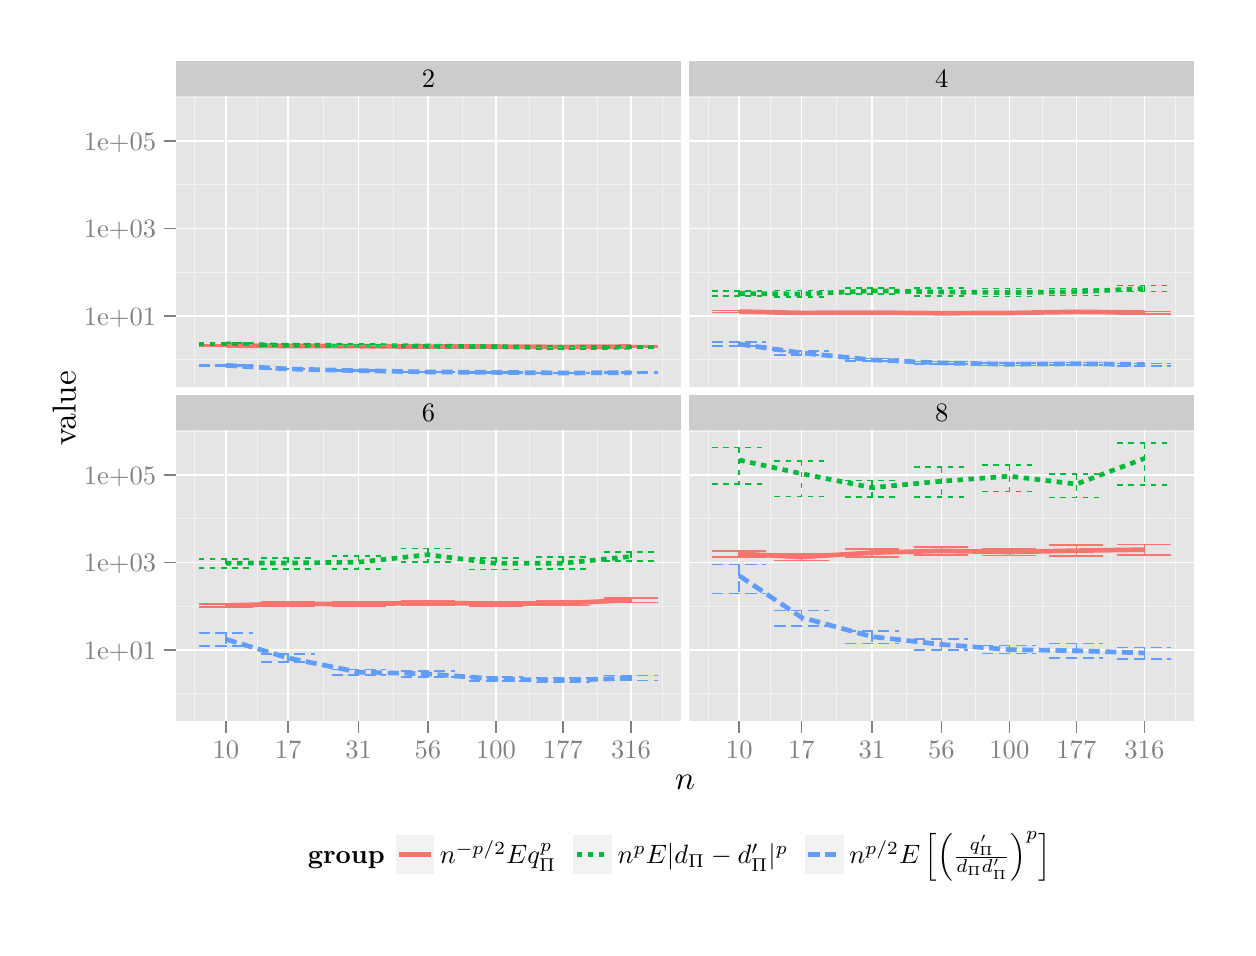
\begin{tikzpicture}[x=1pt,y=1pt]
\definecolor[named]{fillColor}{rgb}{1.00,1.00,1.00}
\path[use as bounding box,fill=fillColor,fill opacity=0.00] (0,0) rectangle (433.62,325.21);
\begin{scope}
\path[clip] (  0.00,  0.00) rectangle (433.62,325.21);
\definecolor[named]{drawColor}{rgb}{1.00,1.00,1.00}
\definecolor[named]{fillColor}{rgb}{1.00,1.00,1.00}

\path[draw=drawColor,line width= 0.6pt,line join=round,line cap=round,fill=fillColor] (  0.00,  0.00) rectangle (433.62,325.21);
\end{scope}
\begin{scope}
\path[clip] ( 53.55,195.47) rectangle (236.06,300.54);
\definecolor[named]{fillColor}{rgb}{0.90,0.90,0.90}

\path[fill=fillColor] ( 53.55,195.47) rectangle (236.06,300.54);
\definecolor[named]{drawColor}{rgb}{0.95,0.95,0.95}

\path[draw=drawColor,line width= 0.3pt,line join=round] ( 53.55,205.20) --
	(236.06,205.20);

\path[draw=drawColor,line width= 0.3pt,line join=round] ( 53.55,236.83) --
	(236.06,236.83);

\path[draw=drawColor,line width= 0.3pt,line join=round] ( 53.55,268.47) --
	(236.06,268.47);

\path[draw=drawColor,line width= 0.3pt,line join=round] ( 53.55,300.11) --
	(236.06,300.11);

\path[draw=drawColor,line width= 0.3pt,line join=round] ( 60.36,195.47) --
	( 60.36,300.54);

\path[draw=drawColor,line width= 0.3pt,line join=round] ( 82.85,195.47) --
	( 82.85,300.54);

\path[draw=drawColor,line width= 0.3pt,line join=round] (106.84,195.47) --
	(106.84,300.54);

\path[draw=drawColor,line width= 0.3pt,line join=round] (132.11,195.47) --
	(132.11,300.54);

\path[draw=drawColor,line width= 0.3pt,line join=round] (156.93,195.47) --
	(156.93,300.54);

\path[draw=drawColor,line width= 0.3pt,line join=round] (181.33,195.47) --
	(181.33,300.54);

\path[draw=drawColor,line width= 0.3pt,line join=round] (205.71,195.47) --
	(205.71,300.54);

\path[draw=drawColor,line width= 0.3pt,line join=round] (229.25,195.47) --
	(229.25,300.54);
\definecolor[named]{drawColor}{rgb}{1.00,1.00,1.00}

\path[draw=drawColor,line width= 0.6pt,line join=round] ( 53.55,221.02) --
	(236.06,221.02);

\path[draw=drawColor,line width= 0.6pt,line join=round] ( 53.55,252.65) --
	(236.06,252.65);

\path[draw=drawColor,line width= 0.6pt,line join=round] ( 53.55,284.29) --
	(236.06,284.29);

\path[draw=drawColor,line width= 0.6pt,line join=round] ( 71.61,195.47) --
	( 71.61,300.54);

\path[draw=drawColor,line width= 0.6pt,line join=round] ( 94.10,195.47) --
	( 94.10,300.54);

\path[draw=drawColor,line width= 0.6pt,line join=round] (119.57,195.47) --
	(119.57,300.54);

\path[draw=drawColor,line width= 0.6pt,line join=round] (144.64,195.47) --
	(144.64,300.54);

\path[draw=drawColor,line width= 0.6pt,line join=round] (169.22,195.47) --
	(169.22,300.54);

\path[draw=drawColor,line width= 0.6pt,line join=round] (193.43,195.47) --
	(193.43,300.54);

\path[draw=drawColor,line width= 0.6pt,line join=round] (218.00,195.47) --
	(218.00,300.54);
\definecolor[named]{drawColor}{rgb}{0.97,0.46,0.43}

\path[draw=drawColor,line width= 1.7pt,line join=round] ( 71.61,210.34) --
	( 94.10,210.19) --
	(119.57,210.13) --
	(144.64,209.96) --
	(169.22,209.97) --
	(193.43,209.84) --
	(218.00,209.99);
\definecolor[named]{drawColor}{rgb}{0.00,0.73,0.22}

\path[draw=drawColor,line width= 1.7pt,dash pattern=on 2pt off 2pt ,line join=round] ( 71.61,210.91) --
	( 94.10,210.43) --
	(119.57,210.41) --
	(144.64,210.16) --
	(169.22,209.92) --
	(193.43,209.58) --
	(218.00,209.71);
\definecolor[named]{drawColor}{rgb}{0.38,0.61,1.00}

\path[draw=drawColor,line width= 1.7pt,dash pattern=on 4pt off 2pt ,line join=round] ( 71.61,203.17) --
	( 94.10,201.88) --
	(119.57,201.26) --
	(144.64,200.81) --
	(169.22,200.64) --
	(193.43,200.43) --
	(218.00,200.54);
\definecolor[named]{drawColor}{rgb}{0.97,0.46,0.43}

\path[draw=drawColor,line width= 0.6pt,line join=round] ( 61.85,210.51) --
	( 81.37,210.51);

\path[draw=drawColor,line width= 0.6pt,line join=round] ( 71.61,210.51) --
	( 71.61,210.16);

\path[draw=drawColor,line width= 0.6pt,line join=round] ( 61.85,210.16) --
	( 81.37,210.16);

\path[draw=drawColor,line width= 0.6pt,line join=round] ( 84.34,210.35) --
	(103.86,210.35);

\path[draw=drawColor,line width= 0.6pt,line join=round] ( 94.10,210.35) --
	( 94.10,210.00);

\path[draw=drawColor,line width= 0.6pt,line join=round] ( 84.34,210.00) --
	(103.86,210.00);

\path[draw=drawColor,line width= 0.6pt,line join=round] (109.81,210.33) --
	(129.33,210.33);

\path[draw=drawColor,line width= 0.6pt,line join=round] (119.57,210.33) --
	(119.57,209.95);

\path[draw=drawColor,line width= 0.6pt,line join=round] (109.81,209.95) --
	(129.33,209.95);

\path[draw=drawColor,line width= 0.6pt,line join=round] (134.88,210.15) --
	(154.40,210.15);

\path[draw=drawColor,line width= 0.6pt,line join=round] (144.64,210.15) --
	(144.64,209.79);

\path[draw=drawColor,line width= 0.6pt,line join=round] (134.88,209.79) --
	(154.40,209.79);

\path[draw=drawColor,line width= 0.6pt,line join=round] (159.46,210.16) --
	(178.98,210.16);

\path[draw=drawColor,line width= 0.6pt,line join=round] (169.22,210.16) --
	(169.22,209.78);

\path[draw=drawColor,line width= 0.6pt,line join=round] (159.46,209.78) --
	(178.98,209.78);

\path[draw=drawColor,line width= 0.6pt,line join=round] (183.67,210.03) --
	(203.19,210.03);

\path[draw=drawColor,line width= 0.6pt,line join=round] (193.43,210.03) --
	(193.43,209.66);

\path[draw=drawColor,line width= 0.6pt,line join=round] (183.67,209.66) --
	(203.19,209.66);

\path[draw=drawColor,line width= 0.6pt,line join=round] (208.24,210.18) --
	(227.76,210.18);

\path[draw=drawColor,line width= 0.6pt,line join=round] (218.00,210.18) --
	(218.00,209.80);

\path[draw=drawColor,line width= 0.6pt,line join=round] (208.24,209.80) --
	(227.76,209.80);
\definecolor[named]{drawColor}{rgb}{0.00,0.73,0.22}

\path[draw=drawColor,line width= 0.6pt,dash pattern=on 2pt off 2pt ,line join=round] ( 61.85,211.25) --
	( 81.37,211.25);

\path[draw=drawColor,line width= 0.6pt,dash pattern=on 2pt off 2pt ,line join=round] ( 71.61,211.25) --
	( 71.61,210.58);

\path[draw=drawColor,line width= 0.6pt,dash pattern=on 2pt off 2pt ,line join=round] ( 61.85,210.58) --
	( 81.37,210.58);

\path[draw=drawColor,line width= 0.6pt,dash pattern=on 2pt off 2pt ,line join=round] ( 84.34,210.80) --
	(103.86,210.80);

\path[draw=drawColor,line width= 0.6pt,dash pattern=on 2pt off 2pt ,line join=round] ( 94.10,210.80) --
	( 94.10,210.09);

\path[draw=drawColor,line width= 0.6pt,dash pattern=on 2pt off 2pt ,line join=round] ( 84.34,210.09) --
	(103.86,210.09);

\path[draw=drawColor,line width= 0.6pt,dash pattern=on 2pt off 2pt ,line join=round] (109.81,210.72) --
	(129.33,210.72);

\path[draw=drawColor,line width= 0.6pt,dash pattern=on 2pt off 2pt ,line join=round] (119.57,210.72) --
	(119.57,210.05);

\path[draw=drawColor,line width= 0.6pt,dash pattern=on 2pt off 2pt ,line join=round] (109.81,210.05) --
	(129.33,210.05);

\path[draw=drawColor,line width= 0.6pt,dash pattern=on 2pt off 2pt ,line join=round] (134.88,210.51) --
	(154.40,210.51);

\path[draw=drawColor,line width= 0.6pt,dash pattern=on 2pt off 2pt ,line join=round] (144.64,210.51) --
	(144.64,209.82);

\path[draw=drawColor,line width= 0.6pt,dash pattern=on 2pt off 2pt ,line join=round] (134.88,209.82) --
	(154.40,209.82);

\path[draw=drawColor,line width= 0.6pt,dash pattern=on 2pt off 2pt ,line join=round] (159.46,210.23) --
	(178.98,210.23);

\path[draw=drawColor,line width= 0.6pt,dash pattern=on 2pt off 2pt ,line join=round] (169.22,210.23) --
	(169.22,209.58);

\path[draw=drawColor,line width= 0.6pt,dash pattern=on 2pt off 2pt ,line join=round] (159.46,209.58) --
	(178.98,209.58);

\path[draw=drawColor,line width= 0.6pt,dash pattern=on 2pt off 2pt ,line join=round] (183.67,209.94) --
	(203.19,209.94);

\path[draw=drawColor,line width= 0.6pt,dash pattern=on 2pt off 2pt ,line join=round] (193.43,209.94) --
	(193.43,209.19);

\path[draw=drawColor,line width= 0.6pt,dash pattern=on 2pt off 2pt ,line join=round] (183.67,209.19) --
	(203.19,209.19);

\path[draw=drawColor,line width= 0.6pt,dash pattern=on 2pt off 2pt ,line join=round] (208.24,210.08) --
	(227.76,210.08);

\path[draw=drawColor,line width= 0.6pt,dash pattern=on 2pt off 2pt ,line join=round] (218.00,210.08) --
	(218.00,209.36);

\path[draw=drawColor,line width= 0.6pt,dash pattern=on 2pt off 2pt ,line join=round] (208.24,209.36) --
	(227.76,209.36);
\definecolor[named]{drawColor}{rgb}{0.38,0.61,1.00}

\path[draw=drawColor,line width= 0.6pt,dash pattern=on 4pt off 2pt ,line join=round] ( 61.85,203.43) --
	( 81.37,203.43);

\path[draw=drawColor,line width= 0.6pt,dash pattern=on 4pt off 2pt ,line join=round] ( 71.61,203.43) --
	( 71.61,202.92);

\path[draw=drawColor,line width= 0.6pt,dash pattern=on 4pt off 2pt ,line join=round] ( 61.85,202.92) --
	( 81.37,202.92);

\path[draw=drawColor,line width= 0.6pt,dash pattern=on 4pt off 2pt ,line join=round] ( 84.34,202.11) --
	(103.86,202.11);

\path[draw=drawColor,line width= 0.6pt,dash pattern=on 4pt off 2pt ,line join=round] ( 94.10,202.11) --
	( 94.10,201.68);

\path[draw=drawColor,line width= 0.6pt,dash pattern=on 4pt off 2pt ,line join=round] ( 84.34,201.68) --
	(103.86,201.68);

\path[draw=drawColor,line width= 0.6pt,dash pattern=on 4pt off 2pt ,line join=round] (109.81,201.47) --
	(129.33,201.47);

\path[draw=drawColor,line width= 0.6pt,dash pattern=on 4pt off 2pt ,line join=round] (119.57,201.47) --
	(119.57,201.03);

\path[draw=drawColor,line width= 0.6pt,dash pattern=on 4pt off 2pt ,line join=round] (109.81,201.03) --
	(129.33,201.03);

\path[draw=drawColor,line width= 0.6pt,dash pattern=on 4pt off 2pt ,line join=round] (134.88,201.01) --
	(154.40,201.01);

\path[draw=drawColor,line width= 0.6pt,dash pattern=on 4pt off 2pt ,line join=round] (144.64,201.01) --
	(144.64,200.61);

\path[draw=drawColor,line width= 0.6pt,dash pattern=on 4pt off 2pt ,line join=round] (134.88,200.61) --
	(154.40,200.61);

\path[draw=drawColor,line width= 0.6pt,dash pattern=on 4pt off 2pt ,line join=round] (159.46,200.84) --
	(178.98,200.84);

\path[draw=drawColor,line width= 0.6pt,dash pattern=on 4pt off 2pt ,line join=round] (169.22,200.84) --
	(169.22,200.47);

\path[draw=drawColor,line width= 0.6pt,dash pattern=on 4pt off 2pt ,line join=round] (159.46,200.47) --
	(178.98,200.47);

\path[draw=drawColor,line width= 0.6pt,dash pattern=on 4pt off 2pt ,line join=round] (183.67,200.63) --
	(203.19,200.63);

\path[draw=drawColor,line width= 0.6pt,dash pattern=on 4pt off 2pt ,line join=round] (193.43,200.63) --
	(193.43,200.25);

\path[draw=drawColor,line width= 0.6pt,dash pattern=on 4pt off 2pt ,line join=round] (183.67,200.25) --
	(203.19,200.25);

\path[draw=drawColor,line width= 0.6pt,dash pattern=on 4pt off 2pt ,line join=round] (208.24,200.72) --
	(227.76,200.72);

\path[draw=drawColor,line width= 0.6pt,dash pattern=on 4pt off 2pt ,line join=round] (218.00,200.72) --
	(218.00,200.35);

\path[draw=drawColor,line width= 0.6pt,dash pattern=on 4pt off 2pt ,line join=round] (208.24,200.35) --
	(227.76,200.35);
\end{scope}
\begin{scope}
\path[clip] (239.07,195.47) rectangle (421.58,300.54);
\definecolor[named]{fillColor}{rgb}{0.90,0.90,0.90}

\path[fill=fillColor] (239.07,195.47) rectangle (421.57,300.54);
\definecolor[named]{drawColor}{rgb}{0.95,0.95,0.95}

\path[draw=drawColor,line width= 0.3pt,line join=round] (239.07,205.20) --
	(421.58,205.20);

\path[draw=drawColor,line width= 0.3pt,line join=round] (239.07,236.83) --
	(421.58,236.83);

\path[draw=drawColor,line width= 0.3pt,line join=round] (239.07,268.47) --
	(421.58,268.47);

\path[draw=drawColor,line width= 0.3pt,line join=round] (239.07,300.11) --
	(421.58,300.11);

\path[draw=drawColor,line width= 0.3pt,line join=round] (245.88,195.47) --
	(245.88,300.54);

\path[draw=drawColor,line width= 0.3pt,line join=round] (268.37,195.47) --
	(268.37,300.54);

\path[draw=drawColor,line width= 0.3pt,line join=round] (292.36,195.47) --
	(292.36,300.54);

\path[draw=drawColor,line width= 0.3pt,line join=round] (317.62,195.47) --
	(317.62,300.54);

\path[draw=drawColor,line width= 0.3pt,line join=round] (342.45,195.47) --
	(342.45,300.54);

\path[draw=drawColor,line width= 0.3pt,line join=round] (366.84,195.47) --
	(366.84,300.54);

\path[draw=drawColor,line width= 0.3pt,line join=round] (391.23,195.47) --
	(391.23,300.54);

\path[draw=drawColor,line width= 0.3pt,line join=round] (414.77,195.47) --
	(414.77,300.54);
\definecolor[named]{drawColor}{rgb}{1.00,1.00,1.00}

\path[draw=drawColor,line width= 0.6pt,line join=round] (239.07,221.02) --
	(421.58,221.02);

\path[draw=drawColor,line width= 0.6pt,line join=round] (239.07,252.65) --
	(421.58,252.65);

\path[draw=drawColor,line width= 0.6pt,line join=round] (239.07,284.29) --
	(421.58,284.29);

\path[draw=drawColor,line width= 0.6pt,line join=round] (257.13,195.47) --
	(257.13,300.54);

\path[draw=drawColor,line width= 0.6pt,line join=round] (279.62,195.47) --
	(279.62,300.54);

\path[draw=drawColor,line width= 0.6pt,line join=round] (305.09,195.47) --
	(305.09,300.54);

\path[draw=drawColor,line width= 0.6pt,line join=round] (330.16,195.47) --
	(330.16,300.54);

\path[draw=drawColor,line width= 0.6pt,line join=round] (354.74,195.47) --
	(354.74,300.54);

\path[draw=drawColor,line width= 0.6pt,line join=round] (378.95,195.47) --
	(378.95,300.54);

\path[draw=drawColor,line width= 0.6pt,line join=round] (403.52,195.47) --
	(403.52,300.54);
\definecolor[named]{drawColor}{rgb}{0.97,0.46,0.43}

\path[draw=drawColor,line width= 1.7pt,line join=round] (257.13,222.62) --
	(279.62,222.14) --
	(305.09,222.23) --
	(330.16,222.03) --
	(354.74,222.11) --
	(378.95,222.52) --
	(403.52,222.27);
\definecolor[named]{drawColor}{rgb}{0.00,0.73,0.22}

\path[draw=drawColor,line width= 1.7pt,dash pattern=on 2pt off 2pt ,line join=round] (257.13,229.13) --
	(279.62,228.99) --
	(305.09,230.12) --
	(330.16,229.70) --
	(354.74,229.48) --
	(378.95,229.77) --
	(403.52,230.93);
\definecolor[named]{drawColor}{rgb}{0.38,0.61,1.00}

\path[draw=drawColor,line width= 1.7pt,dash pattern=on 4pt off 2pt ,line join=round] (257.13,210.85) --
	(279.62,207.69) --
	(305.09,205.17) --
	(330.16,204.07) --
	(354.74,203.59) --
	(378.95,203.75) --
	(403.52,203.49);
\definecolor[named]{drawColor}{rgb}{0.97,0.46,0.43}

\path[draw=drawColor,line width= 0.6pt,line join=round] (247.36,222.99) --
	(266.89,222.99);

\path[draw=drawColor,line width= 0.6pt,line join=round] (257.13,222.99) --
	(257.13,222.28);

\path[draw=drawColor,line width= 0.6pt,line join=round] (247.36,222.28) --
	(266.89,222.28);

\path[draw=drawColor,line width= 0.6pt,line join=round] (269.86,222.51) --
	(289.38,222.51);

\path[draw=drawColor,line width= 0.6pt,line join=round] (279.62,222.51) --
	(279.62,221.73);

\path[draw=drawColor,line width= 0.6pt,line join=round] (269.86,221.73) --
	(289.38,221.73);

\path[draw=drawColor,line width= 0.6pt,line join=round] (295.33,222.61) --
	(314.85,222.61);

\path[draw=drawColor,line width= 0.6pt,line join=round] (305.09,222.61) --
	(305.09,221.83);

\path[draw=drawColor,line width= 0.6pt,line join=round] (295.33,221.83) --
	(314.85,221.83);

\path[draw=drawColor,line width= 0.6pt,line join=round] (320.40,222.45) --
	(339.92,222.45);

\path[draw=drawColor,line width= 0.6pt,line join=round] (330.16,222.45) --
	(330.16,221.63);

\path[draw=drawColor,line width= 0.6pt,line join=round] (320.40,221.63) --
	(339.92,221.63);

\path[draw=drawColor,line width= 0.6pt,line join=round] (344.98,222.54) --
	(364.50,222.54);

\path[draw=drawColor,line width= 0.6pt,line join=round] (354.74,222.54) --
	(354.74,221.64);

\path[draw=drawColor,line width= 0.6pt,line join=round] (344.98,221.64) --
	(364.50,221.64);

\path[draw=drawColor,line width= 0.6pt,line join=round] (369.19,222.94) --
	(388.71,222.94);

\path[draw=drawColor,line width= 0.6pt,line join=round] (378.95,222.94) --
	(378.95,222.08);

\path[draw=drawColor,line width= 0.6pt,line join=round] (369.19,222.08) --
	(388.71,222.08);

\path[draw=drawColor,line width= 0.6pt,line join=round] (393.76,222.69) --
	(413.28,222.69);

\path[draw=drawColor,line width= 0.6pt,line join=round] (403.52,222.69) --
	(403.52,221.83);

\path[draw=drawColor,line width= 0.6pt,line join=round] (393.76,221.83) --
	(413.28,221.83);
\definecolor[named]{drawColor}{rgb}{0.00,0.73,0.22}

\path[draw=drawColor,line width= 0.6pt,dash pattern=on 2pt off 2pt ,line join=round] (247.36,230.03) --
	(266.89,230.03);

\path[draw=drawColor,line width= 0.6pt,dash pattern=on 2pt off 2pt ,line join=round] (257.13,230.03) --
	(257.13,228.13);

\path[draw=drawColor,line width= 0.6pt,dash pattern=on 2pt off 2pt ,line join=round] (247.36,228.13) --
	(266.89,228.13);

\path[draw=drawColor,line width= 0.6pt,dash pattern=on 2pt off 2pt ,line join=round] (269.86,230.18) --
	(289.38,230.18);

\path[draw=drawColor,line width= 0.6pt,dash pattern=on 2pt off 2pt ,line join=round] (279.62,230.18) --
	(279.62,227.77);

\path[draw=drawColor,line width= 0.6pt,dash pattern=on 2pt off 2pt ,line join=round] (269.86,227.77) --
	(289.38,227.77);

\path[draw=drawColor,line width= 0.6pt,dash pattern=on 2pt off 2pt ,line join=round] (295.33,231.20) --
	(314.85,231.20);

\path[draw=drawColor,line width= 0.6pt,dash pattern=on 2pt off 2pt ,line join=round] (305.09,231.20) --
	(305.09,228.92);

\path[draw=drawColor,line width= 0.6pt,dash pattern=on 2pt off 2pt ,line join=round] (295.33,228.92) --
	(314.85,228.92);

\path[draw=drawColor,line width= 0.6pt,dash pattern=on 2pt off 2pt ,line join=round] (320.40,231.12) --
	(339.92,231.12);

\path[draw=drawColor,line width= 0.6pt,dash pattern=on 2pt off 2pt ,line join=round] (330.16,231.12) --
	(330.16,228.31);

\path[draw=drawColor,line width= 0.6pt,dash pattern=on 2pt off 2pt ,line join=round] (320.40,228.31) --
	(339.92,228.31);

\path[draw=drawColor,line width= 0.6pt,dash pattern=on 2pt off 2pt ,line join=round] (344.98,230.90) --
	(364.50,230.90);

\path[draw=drawColor,line width= 0.6pt,dash pattern=on 2pt off 2pt ,line join=round] (354.74,230.90) --
	(354.74,228.11);

\path[draw=drawColor,line width= 0.6pt,dash pattern=on 2pt off 2pt ,line join=round] (344.98,228.11) --
	(364.50,228.11);

\path[draw=drawColor,line width= 0.6pt,dash pattern=on 2pt off 2pt ,line join=round] (369.19,231.00) --
	(388.71,231.00);

\path[draw=drawColor,line width= 0.6pt,dash pattern=on 2pt off 2pt ,line join=round] (378.95,231.00) --
	(378.95,228.43);

\path[draw=drawColor,line width= 0.6pt,dash pattern=on 2pt off 2pt ,line join=round] (369.19,228.43) --
	(388.71,228.43);

\path[draw=drawColor,line width= 0.6pt,dash pattern=on 2pt off 2pt ,line join=round] (393.76,232.03) --
	(413.28,232.03);

\path[draw=drawColor,line width= 0.6pt,dash pattern=on 2pt off 2pt ,line join=round] (403.52,232.03) --
	(403.52,229.82);

\path[draw=drawColor,line width= 0.6pt,dash pattern=on 2pt off 2pt ,line join=round] (393.76,229.82) --
	(413.28,229.82);
\definecolor[named]{drawColor}{rgb}{0.38,0.61,1.00}

\path[draw=drawColor,line width= 0.6pt,dash pattern=on 4pt off 2pt ,line join=round] (247.36,211.60) --
	(266.89,211.60);

\path[draw=drawColor,line width= 0.6pt,dash pattern=on 4pt off 2pt ,line join=round] (257.13,211.60) --
	(257.13,210.09);

\path[draw=drawColor,line width= 0.6pt,dash pattern=on 4pt off 2pt ,line join=round] (247.36,210.09) --
	(266.89,210.09);

\path[draw=drawColor,line width= 0.6pt,dash pattern=on 4pt off 2pt ,line join=round] (269.86,208.37) --
	(289.38,208.37);

\path[draw=drawColor,line width= 0.6pt,dash pattern=on 4pt off 2pt ,line join=round] (279.62,208.37) --
	(279.62,206.97);

\path[draw=drawColor,line width= 0.6pt,dash pattern=on 4pt off 2pt ,line join=round] (269.86,206.97) --
	(289.38,206.97);

\path[draw=drawColor,line width= 0.6pt,dash pattern=on 4pt off 2pt ,line join=round] (295.33,205.66) --
	(314.85,205.66);

\path[draw=drawColor,line width= 0.6pt,dash pattern=on 4pt off 2pt ,line join=round] (305.09,205.66) --
	(305.09,204.66);

\path[draw=drawColor,line width= 0.6pt,dash pattern=on 4pt off 2pt ,line join=round] (295.33,204.66) --
	(314.85,204.66);

\path[draw=drawColor,line width= 0.6pt,dash pattern=on 4pt off 2pt ,line join=round] (320.40,204.59) --
	(339.92,204.59);

\path[draw=drawColor,line width= 0.6pt,dash pattern=on 4pt off 2pt ,line join=round] (330.16,204.59) --
	(330.16,203.56);

\path[draw=drawColor,line width= 0.6pt,dash pattern=on 4pt off 2pt ,line join=round] (320.40,203.56) --
	(339.92,203.56);

\path[draw=drawColor,line width= 0.6pt,dash pattern=on 4pt off 2pt ,line join=round] (344.98,204.02) --
	(364.50,204.02);

\path[draw=drawColor,line width= 0.6pt,dash pattern=on 4pt off 2pt ,line join=round] (354.74,204.02) --
	(354.74,203.11);

\path[draw=drawColor,line width= 0.6pt,dash pattern=on 4pt off 2pt ,line join=round] (344.98,203.11) --
	(364.50,203.11);

\path[draw=drawColor,line width= 0.6pt,dash pattern=on 4pt off 2pt ,line join=round] (369.19,204.19) --
	(388.71,204.19);

\path[draw=drawColor,line width= 0.6pt,dash pattern=on 4pt off 2pt ,line join=round] (378.95,204.19) --
	(378.95,203.31);

\path[draw=drawColor,line width= 0.6pt,dash pattern=on 4pt off 2pt ,line join=round] (369.19,203.31) --
	(388.71,203.31);

\path[draw=drawColor,line width= 0.6pt,dash pattern=on 4pt off 2pt ,line join=round] (393.76,203.89) --
	(413.28,203.89);

\path[draw=drawColor,line width= 0.6pt,dash pattern=on 4pt off 2pt ,line join=round] (403.52,203.89) --
	(403.52,203.07);

\path[draw=drawColor,line width= 0.6pt,dash pattern=on 4pt off 2pt ,line join=round] (393.76,203.07) --
	(413.28,203.07);
\end{scope}
\begin{scope}
\path[clip] ( 53.55, 74.76) rectangle (236.06,179.83);
\definecolor[named]{fillColor}{rgb}{0.90,0.90,0.90}

\path[fill=fillColor] ( 53.55, 74.76) rectangle (236.06,179.83);
\definecolor[named]{drawColor}{rgb}{0.95,0.95,0.95}

\path[draw=drawColor,line width= 0.3pt,line join=round] ( 53.55, 84.48) --
	(236.06, 84.48);

\path[draw=drawColor,line width= 0.3pt,line join=round] ( 53.55,116.12) --
	(236.06,116.12);

\path[draw=drawColor,line width= 0.3pt,line join=round] ( 53.55,147.76) --
	(236.06,147.76);

\path[draw=drawColor,line width= 0.3pt,line join=round] ( 53.55,179.40) --
	(236.06,179.40);

\path[draw=drawColor,line width= 0.3pt,line join=round] ( 60.36, 74.76) --
	( 60.36,179.83);

\path[draw=drawColor,line width= 0.3pt,line join=round] ( 82.85, 74.76) --
	( 82.85,179.83);

\path[draw=drawColor,line width= 0.3pt,line join=round] (106.84, 74.76) --
	(106.84,179.83);

\path[draw=drawColor,line width= 0.3pt,line join=round] (132.11, 74.76) --
	(132.11,179.83);

\path[draw=drawColor,line width= 0.3pt,line join=round] (156.93, 74.76) --
	(156.93,179.83);

\path[draw=drawColor,line width= 0.3pt,line join=round] (181.33, 74.76) --
	(181.33,179.83);

\path[draw=drawColor,line width= 0.3pt,line join=round] (205.71, 74.76) --
	(205.71,179.83);

\path[draw=drawColor,line width= 0.3pt,line join=round] (229.25, 74.76) --
	(229.25,179.83);
\definecolor[named]{drawColor}{rgb}{1.00,1.00,1.00}

\path[draw=drawColor,line width= 0.6pt,line join=round] ( 53.55,100.30) --
	(236.06,100.30);

\path[draw=drawColor,line width= 0.6pt,line join=round] ( 53.55,131.94) --
	(236.06,131.94);

\path[draw=drawColor,line width= 0.6pt,line join=round] ( 53.55,163.58) --
	(236.06,163.58);

\path[draw=drawColor,line width= 0.6pt,line join=round] ( 71.61, 74.76) --
	( 71.61,179.83);

\path[draw=drawColor,line width= 0.6pt,line join=round] ( 94.10, 74.76) --
	( 94.10,179.83);

\path[draw=drawColor,line width= 0.6pt,line join=round] (119.57, 74.76) --
	(119.57,179.83);

\path[draw=drawColor,line width= 0.6pt,line join=round] (144.64, 74.76) --
	(144.64,179.83);

\path[draw=drawColor,line width= 0.6pt,line join=round] (169.22, 74.76) --
	(169.22,179.83);

\path[draw=drawColor,line width= 0.6pt,line join=round] (193.43, 74.76) --
	(193.43,179.83);

\path[draw=drawColor,line width= 0.6pt,line join=round] (218.00, 74.76) --
	(218.00,179.83);
\definecolor[named]{drawColor}{rgb}{0.97,0.46,0.43}

\path[draw=drawColor,line width= 1.7pt,line join=round] ( 71.61,116.42) --
	( 94.10,117.02) --
	(119.57,116.96) --
	(144.64,117.35) --
	(169.22,117.07) --
	(193.43,117.18) --
	(218.00,118.40);
\definecolor[named]{drawColor}{rgb}{0.00,0.73,0.22}

\path[draw=drawColor,line width= 1.7pt,dash pattern=on 2pt off 2pt ,line join=round] ( 71.61,131.71) --
	( 94.10,131.77) --
	(119.57,132.07) --
	(144.64,134.77) --
	(169.22,131.62) --
	(193.43,131.70) --
	(218.00,134.11);
\definecolor[named]{drawColor}{rgb}{0.38,0.61,1.00}

\path[draw=drawColor,line width= 1.7pt,dash pattern=on 4pt off 2pt ,line join=round] ( 71.61,104.20) --
	( 94.10, 97.44) --
	(119.57, 92.33) --
	(144.64, 91.70) --
	(169.22, 89.83) --
	(193.43, 89.37) --
	(218.00, 90.18);
\definecolor[named]{drawColor}{rgb}{0.97,0.46,0.43}

\path[draw=drawColor,line width= 0.6pt,line join=round] ( 61.85,117.04) --
	( 81.37,117.04);

\path[draw=drawColor,line width= 0.6pt,line join=round] ( 71.61,117.04) --
	( 71.61,115.81);

\path[draw=drawColor,line width= 0.6pt,line join=round] ( 61.85,115.81) --
	( 81.37,115.81);

\path[draw=drawColor,line width= 0.6pt,line join=round] ( 84.34,117.67) --
	(103.86,117.67);

\path[draw=drawColor,line width= 0.6pt,line join=round] ( 94.10,117.67) --
	( 94.10,116.25);

\path[draw=drawColor,line width= 0.6pt,line join=round] ( 84.34,116.25) --
	(103.86,116.25);

\path[draw=drawColor,line width= 0.6pt,line join=round] (109.81,117.61) --
	(129.33,117.61);

\path[draw=drawColor,line width= 0.6pt,line join=round] (119.57,117.61) --
	(119.57,116.20);

\path[draw=drawColor,line width= 0.6pt,line join=round] (109.81,116.20) --
	(129.33,116.20);

\path[draw=drawColor,line width= 0.6pt,line join=round] (134.88,118.24) --
	(154.40,118.24);

\path[draw=drawColor,line width= 0.6pt,line join=round] (144.64,118.24) --
	(144.64,116.48);

\path[draw=drawColor,line width= 0.6pt,line join=round] (134.88,116.48) --
	(154.40,116.48);

\path[draw=drawColor,line width= 0.6pt,line join=round] (159.46,117.80) --
	(178.98,117.80);

\path[draw=drawColor,line width= 0.6pt,line join=round] (169.22,117.80) --
	(169.22,116.30);

\path[draw=drawColor,line width= 0.6pt,line join=round] (159.46,116.30) --
	(178.98,116.30);

\path[draw=drawColor,line width= 0.6pt,line join=round] (183.67,118.00) --
	(203.19,118.00);

\path[draw=drawColor,line width= 0.6pt,line join=round] (193.43,118.00) --
	(193.43,116.35);

\path[draw=drawColor,line width= 0.6pt,line join=round] (183.67,116.35) --
	(203.19,116.35);

\path[draw=drawColor,line width= 0.6pt,line join=round] (208.24,119.23) --
	(227.76,119.23);

\path[draw=drawColor,line width= 0.6pt,line join=round] (218.00,119.23) --
	(218.00,117.50);

\path[draw=drawColor,line width= 0.6pt,line join=round] (208.24,117.50) --
	(227.76,117.50);
\definecolor[named]{drawColor}{rgb}{0.00,0.73,0.22}

\path[draw=drawColor,line width= 0.6pt,dash pattern=on 2pt off 2pt ,line join=round] ( 61.85,133.32) --
	( 81.37,133.32);

\path[draw=drawColor,line width= 0.6pt,dash pattern=on 2pt off 2pt ,line join=round] ( 71.61,133.32) --
	( 71.61,130.06);

\path[draw=drawColor,line width= 0.6pt,dash pattern=on 2pt off 2pt ,line join=round] ( 61.85,130.06) --
	( 81.37,130.06);

\path[draw=drawColor,line width= 0.6pt,dash pattern=on 2pt off 2pt ,line join=round] ( 84.34,133.65) --
	(103.86,133.65);

\path[draw=drawColor,line width= 0.6pt,dash pattern=on 2pt off 2pt ,line join=round] ( 94.10,133.65) --
	( 94.10,129.67);

\path[draw=drawColor,line width= 0.6pt,dash pattern=on 2pt off 2pt ,line join=round] ( 84.34,129.67) --
	(103.86,129.67);

\path[draw=drawColor,line width= 0.6pt,dash pattern=on 2pt off 2pt ,line join=round] (109.81,134.31) --
	(129.33,134.31);

\path[draw=drawColor,line width= 0.6pt,dash pattern=on 2pt off 2pt ,line join=round] (119.57,134.31) --
	(119.57,129.64);

\path[draw=drawColor,line width= 0.6pt,dash pattern=on 2pt off 2pt ,line join=round] (109.81,129.64) --
	(129.33,129.64);

\path[draw=drawColor,line width= 0.6pt,dash pattern=on 2pt off 2pt ,line join=round] (134.88,137.04) --
	(154.40,137.04);

\path[draw=drawColor,line width= 0.6pt,dash pattern=on 2pt off 2pt ,line join=round] (144.64,137.04) --
	(144.64,132.18);

\path[draw=drawColor,line width= 0.6pt,dash pattern=on 2pt off 2pt ,line join=round] (134.88,132.18) --
	(154.40,132.18);

\path[draw=drawColor,line width= 0.6pt,dash pattern=on 2pt off 2pt ,line join=round] (159.46,133.62) --
	(178.98,133.62);

\path[draw=drawColor,line width= 0.6pt,dash pattern=on 2pt off 2pt ,line join=round] (169.22,133.62) --
	(169.22,129.40);

\path[draw=drawColor,line width= 0.6pt,dash pattern=on 2pt off 2pt ,line join=round] (159.46,129.40) --
	(178.98,129.40);

\path[draw=drawColor,line width= 0.6pt,dash pattern=on 2pt off 2pt ,line join=round] (183.67,133.84) --
	(203.19,133.84);

\path[draw=drawColor,line width= 0.6pt,dash pattern=on 2pt off 2pt ,line join=round] (193.43,133.84) --
	(193.43,129.52);

\path[draw=drawColor,line width= 0.6pt,dash pattern=on 2pt off 2pt ,line join=round] (183.67,129.52) --
	(203.19,129.52);

\path[draw=drawColor,line width= 0.6pt,dash pattern=on 2pt off 2pt ,line join=round] (208.24,135.72) --
	(227.76,135.72);

\path[draw=drawColor,line width= 0.6pt,dash pattern=on 2pt off 2pt ,line join=round] (218.00,135.72) --
	(218.00,132.38);

\path[draw=drawColor,line width= 0.6pt,dash pattern=on 2pt off 2pt ,line join=round] (208.24,132.38) --
	(227.76,132.38);
\definecolor[named]{drawColor}{rgb}{0.38,0.61,1.00}

\path[draw=drawColor,line width= 0.6pt,dash pattern=on 4pt off 2pt ,line join=round] ( 61.85,106.46) --
	( 81.37,106.46);

\path[draw=drawColor,line width= 0.6pt,dash pattern=on 4pt off 2pt ,line join=round] ( 71.61,106.46) --
	( 71.61,101.85);

\path[draw=drawColor,line width= 0.6pt,dash pattern=on 4pt off 2pt ,line join=round] ( 61.85,101.85) --
	( 81.37,101.85);

\path[draw=drawColor,line width= 0.6pt,dash pattern=on 4pt off 2pt ,line join=round] ( 84.34, 98.79) --
	(103.86, 98.79);

\path[draw=drawColor,line width= 0.6pt,dash pattern=on 4pt off 2pt ,line join=round] ( 94.10, 98.79) --
	( 94.10, 96.10);

\path[draw=drawColor,line width= 0.6pt,dash pattern=on 4pt off 2pt ,line join=round] ( 84.34, 96.10) --
	(103.86, 96.10);

\path[draw=drawColor,line width= 0.6pt,dash pattern=on 4pt off 2pt ,line join=round] (109.81, 93.27) --
	(129.33, 93.27);

\path[draw=drawColor,line width= 0.6pt,dash pattern=on 4pt off 2pt ,line join=round] (119.57, 93.27) --
	(119.57, 91.23);

\path[draw=drawColor,line width= 0.6pt,dash pattern=on 4pt off 2pt ,line join=round] (109.81, 91.23) --
	(129.33, 91.23);

\path[draw=drawColor,line width= 0.6pt,dash pattern=on 4pt off 2pt ,line join=round] (134.88, 92.80) --
	(154.40, 92.80);

\path[draw=drawColor,line width= 0.6pt,dash pattern=on 4pt off 2pt ,line join=round] (144.64, 92.80) --
	(144.64, 90.62);

\path[draw=drawColor,line width= 0.6pt,dash pattern=on 4pt off 2pt ,line join=round] (134.88, 90.62) --
	(154.40, 90.62);

\path[draw=drawColor,line width= 0.6pt,dash pattern=on 4pt off 2pt ,line join=round] (159.46, 90.60) --
	(178.98, 90.60);

\path[draw=drawColor,line width= 0.6pt,dash pattern=on 4pt off 2pt ,line join=round] (169.22, 90.60) --
	(169.22, 89.04);

\path[draw=drawColor,line width= 0.6pt,dash pattern=on 4pt off 2pt ,line join=round] (159.46, 89.04) --
	(178.98, 89.04);

\path[draw=drawColor,line width= 0.6pt,dash pattern=on 4pt off 2pt ,line join=round] (183.67, 90.19) --
	(203.19, 90.19);

\path[draw=drawColor,line width= 0.6pt,dash pattern=on 4pt off 2pt ,line join=round] (193.43, 90.19) --
	(193.43, 88.53);

\path[draw=drawColor,line width= 0.6pt,dash pattern=on 4pt off 2pt ,line join=round] (183.67, 88.53) --
	(203.19, 88.53);

\path[draw=drawColor,line width= 0.6pt,dash pattern=on 4pt off 2pt ,line join=round] (208.24, 91.06) --
	(227.76, 91.06);

\path[draw=drawColor,line width= 0.6pt,dash pattern=on 4pt off 2pt ,line join=round] (218.00, 91.06) --
	(218.00, 89.30);

\path[draw=drawColor,line width= 0.6pt,dash pattern=on 4pt off 2pt ,line join=round] (208.24, 89.30) --
	(227.76, 89.30);
\end{scope}
\begin{scope}
\path[clip] (239.07, 74.76) rectangle (421.58,179.83);
\definecolor[named]{fillColor}{rgb}{0.90,0.90,0.90}

\path[fill=fillColor] (239.07, 74.76) rectangle (421.57,179.83);
\definecolor[named]{drawColor}{rgb}{0.95,0.95,0.95}

\path[draw=drawColor,line width= 0.3pt,line join=round] (239.07, 84.48) --
	(421.58, 84.48);

\path[draw=drawColor,line width= 0.3pt,line join=round] (239.07,116.12) --
	(421.58,116.12);

\path[draw=drawColor,line width= 0.3pt,line join=round] (239.07,147.76) --
	(421.58,147.76);

\path[draw=drawColor,line width= 0.3pt,line join=round] (239.07,179.40) --
	(421.58,179.40);

\path[draw=drawColor,line width= 0.3pt,line join=round] (245.88, 74.76) --
	(245.88,179.83);

\path[draw=drawColor,line width= 0.3pt,line join=round] (268.37, 74.76) --
	(268.37,179.83);

\path[draw=drawColor,line width= 0.3pt,line join=round] (292.36, 74.76) --
	(292.36,179.83);

\path[draw=drawColor,line width= 0.3pt,line join=round] (317.62, 74.76) --
	(317.62,179.83);

\path[draw=drawColor,line width= 0.3pt,line join=round] (342.45, 74.76) --
	(342.45,179.83);

\path[draw=drawColor,line width= 0.3pt,line join=round] (366.84, 74.76) --
	(366.84,179.83);

\path[draw=drawColor,line width= 0.3pt,line join=round] (391.23, 74.76) --
	(391.23,179.83);

\path[draw=drawColor,line width= 0.3pt,line join=round] (414.77, 74.76) --
	(414.77,179.83);
\definecolor[named]{drawColor}{rgb}{1.00,1.00,1.00}

\path[draw=drawColor,line width= 0.6pt,line join=round] (239.07,100.30) --
	(421.58,100.30);

\path[draw=drawColor,line width= 0.6pt,line join=round] (239.07,131.94) --
	(421.58,131.94);

\path[draw=drawColor,line width= 0.6pt,line join=round] (239.07,163.58) --
	(421.58,163.58);

\path[draw=drawColor,line width= 0.6pt,line join=round] (257.13, 74.76) --
	(257.13,179.83);

\path[draw=drawColor,line width= 0.6pt,line join=round] (279.62, 74.76) --
	(279.62,179.83);

\path[draw=drawColor,line width= 0.6pt,line join=round] (305.09, 74.76) --
	(305.09,179.83);

\path[draw=drawColor,line width= 0.6pt,line join=round] (330.16, 74.76) --
	(330.16,179.83);

\path[draw=drawColor,line width= 0.6pt,line join=round] (354.74, 74.76) --
	(354.74,179.83);

\path[draw=drawColor,line width= 0.6pt,line join=round] (378.95, 74.76) --
	(378.95,179.83);

\path[draw=drawColor,line width= 0.6pt,line join=round] (403.52, 74.76) --
	(403.52,179.83);
\definecolor[named]{drawColor}{rgb}{0.97,0.46,0.43}

\path[draw=drawColor,line width= 1.7pt,line join=round] (257.13,135.09) --
	(279.62,133.93) --
	(305.09,135.50) --
	(330.16,136.14) --
	(354.74,135.75) --
	(378.95,136.23) --
	(403.52,136.59);
\definecolor[named]{drawColor}{rgb}{0.00,0.73,0.22}

\path[draw=drawColor,line width= 1.7pt,dash pattern=on 2pt off 2pt ,line join=round] (257.13,168.97) --
	(279.62,164.05) --
	(305.09,158.99) --
	(330.16,161.31) --
	(354.74,163.15) --
	(378.95,160.29) --
	(403.52,169.55);
\definecolor[named]{drawColor}{rgb}{0.38,0.61,1.00}

\path[draw=drawColor,line width= 1.7pt,dash pattern=on 4pt off 2pt ,line join=round] (257.13,127.16) --
	(279.62,112.10) --
	(305.09,105.15) --
	(330.16,102.34) --
	(354.74,100.48) --
	(378.95,100.07) --
	(403.52, 99.25);
\definecolor[named]{drawColor}{rgb}{0.97,0.46,0.43}

\path[draw=drawColor,line width= 0.6pt,line join=round] (247.36,136.16) --
	(266.89,136.16);

\path[draw=drawColor,line width= 0.6pt,line join=round] (257.13,136.16) --
	(257.13,133.98);

\path[draw=drawColor,line width= 0.6pt,line join=round] (247.36,133.98) --
	(266.89,133.98);

\path[draw=drawColor,line width= 0.6pt,line join=round] (269.86,135.06) --
	(289.38,135.06);

\path[draw=drawColor,line width= 0.6pt,line join=round] (279.62,135.06) --
	(279.62,132.72);

\path[draw=drawColor,line width= 0.6pt,line join=round] (269.86,132.72) --
	(289.38,132.72);

\path[draw=drawColor,line width= 0.6pt,line join=round] (295.33,136.81) --
	(314.85,136.81);

\path[draw=drawColor,line width= 0.6pt,line join=round] (305.09,136.81) --
	(305.09,133.90);

\path[draw=drawColor,line width= 0.6pt,line join=round] (295.33,133.90) --
	(314.85,133.90);

\path[draw=drawColor,line width= 0.6pt,line join=round] (320.40,137.61) --
	(339.92,137.61);

\path[draw=drawColor,line width= 0.6pt,line join=round] (330.16,137.61) --
	(330.16,134.73);

\path[draw=drawColor,line width= 0.6pt,line join=round] (320.40,134.73) --
	(339.92,134.73);

\path[draw=drawColor,line width= 0.6pt,line join=round] (344.98,136.88) --
	(364.50,136.88);

\path[draw=drawColor,line width= 0.6pt,line join=round] (354.74,136.88) --
	(354.74,134.43);

\path[draw=drawColor,line width= 0.6pt,line join=round] (344.98,134.43) --
	(364.50,134.43);

\path[draw=drawColor,line width= 0.6pt,line join=round] (369.19,138.36) --
	(388.71,138.36);

\path[draw=drawColor,line width= 0.6pt,line join=round] (378.95,138.36) --
	(378.95,134.19);

\path[draw=drawColor,line width= 0.6pt,line join=round] (369.19,134.19) --
	(388.71,134.19);

\path[draw=drawColor,line width= 0.6pt,line join=round] (393.76,138.44) --
	(413.28,138.44);

\path[draw=drawColor,line width= 0.6pt,line join=round] (403.52,138.44) --
	(403.52,134.62);

\path[draw=drawColor,line width= 0.6pt,line join=round] (393.76,134.62) --
	(413.28,134.62);
\definecolor[named]{drawColor}{rgb}{0.00,0.73,0.22}

\path[draw=drawColor,line width= 0.6pt,dash pattern=on 2pt off 2pt ,line join=round] (247.36,173.51) --
	(266.89,173.51);

\path[draw=drawColor,line width= 0.6pt,dash pattern=on 2pt off 2pt ,line join=round] (257.13,173.51) --
	(257.13,160.35);

\path[draw=drawColor,line width= 0.6pt,dash pattern=on 2pt off 2pt ,line join=round] (247.36,160.35) --
	(266.89,160.35);

\path[draw=drawColor,line width= 0.6pt,dash pattern=on 2pt off 2pt ,line join=round] (269.86,168.69) --
	(289.38,168.69);

\path[draw=drawColor,line width= 0.6pt,dash pattern=on 2pt off 2pt ,line join=round] (279.62,168.69) --
	(279.62,155.76);

\path[draw=drawColor,line width= 0.6pt,dash pattern=on 2pt off 2pt ,line join=round] (269.86,155.76) --
	(289.38,155.76);

\path[draw=drawColor,line width= 0.6pt,dash pattern=on 2pt off 2pt ,line join=round] (295.33,161.58) --
	(314.85,161.58);

\path[draw=drawColor,line width= 0.6pt,dash pattern=on 2pt off 2pt ,line join=round] (305.09,161.58) --
	(305.09,155.67);

\path[draw=drawColor,line width= 0.6pt,dash pattern=on 2pt off 2pt ,line join=round] (295.33,155.67) --
	(314.85,155.67);

\path[draw=drawColor,line width= 0.6pt,dash pattern=on 2pt off 2pt ,line join=round] (320.40,166.38) --
	(339.92,166.38);

\path[draw=drawColor,line width= 0.6pt,dash pattern=on 2pt off 2pt ,line join=round] (330.16,166.38) --
	(330.16,155.70);

\path[draw=drawColor,line width= 0.6pt,dash pattern=on 2pt off 2pt ,line join=round] (320.40,155.70) --
	(339.92,155.70);

\path[draw=drawColor,line width= 0.6pt,dash pattern=on 2pt off 2pt ,line join=round] (344.98,167.12) --
	(364.50,167.12);

\path[draw=drawColor,line width= 0.6pt,dash pattern=on 2pt off 2pt ,line join=round] (354.74,167.12) --
	(354.74,157.63);

\path[draw=drawColor,line width= 0.6pt,dash pattern=on 2pt off 2pt ,line join=round] (344.98,157.63) --
	(364.50,157.63);

\path[draw=drawColor,line width= 0.6pt,dash pattern=on 2pt off 2pt ,line join=round] (369.19,163.87) --
	(388.71,163.87);

\path[draw=drawColor,line width= 0.6pt,dash pattern=on 2pt off 2pt ,line join=round] (378.95,163.87) --
	(378.95,155.48);

\path[draw=drawColor,line width= 0.6pt,dash pattern=on 2pt off 2pt ,line join=round] (369.19,155.48) --
	(388.71,155.48);

\path[draw=drawColor,line width= 0.6pt,dash pattern=on 2pt off 2pt ,line join=round] (393.76,175.05) --
	(413.28,175.05);

\path[draw=drawColor,line width= 0.6pt,dash pattern=on 2pt off 2pt ,line join=round] (403.52,175.05) --
	(403.52,160.02);

\path[draw=drawColor,line width= 0.6pt,dash pattern=on 2pt off 2pt ,line join=round] (393.76,160.02) --
	(413.28,160.02);
\definecolor[named]{drawColor}{rgb}{0.38,0.61,1.00}

\path[draw=drawColor,line width= 0.6pt,dash pattern=on 4pt off 2pt ,line join=round] (247.36,131.25) --
	(266.89,131.25);

\path[draw=drawColor,line width= 0.6pt,dash pattern=on 4pt off 2pt ,line join=round] (257.13,131.25) --
	(257.13,120.80);

\path[draw=drawColor,line width= 0.6pt,dash pattern=on 4pt off 2pt ,line join=round] (247.36,120.80) --
	(266.89,120.80);

\path[draw=drawColor,line width= 0.6pt,dash pattern=on 4pt off 2pt ,line join=round] (269.86,114.56) --
	(289.38,114.56);

\path[draw=drawColor,line width= 0.6pt,dash pattern=on 4pt off 2pt ,line join=round] (279.62,114.56) --
	(279.62,109.01);

\path[draw=drawColor,line width= 0.6pt,dash pattern=on 4pt off 2pt ,line join=round] (269.86,109.01) --
	(289.38,109.01);

\path[draw=drawColor,line width= 0.6pt,dash pattern=on 4pt off 2pt ,line join=round] (295.33,107.08) --
	(314.85,107.08);

\path[draw=drawColor,line width= 0.6pt,dash pattern=on 4pt off 2pt ,line join=round] (305.09,107.08) --
	(305.09,102.74);

\path[draw=drawColor,line width= 0.6pt,dash pattern=on 4pt off 2pt ,line join=round] (295.33,102.74) --
	(314.85,102.74);

\path[draw=drawColor,line width= 0.6pt,dash pattern=on 4pt off 2pt ,line join=round] (320.40,104.31) --
	(339.92,104.31);

\path[draw=drawColor,line width= 0.6pt,dash pattern=on 4pt off 2pt ,line join=round] (330.16,104.31) --
	(330.16,100.33);

\path[draw=drawColor,line width= 0.6pt,dash pattern=on 4pt off 2pt ,line join=round] (320.40,100.33) --
	(339.92,100.33);

\path[draw=drawColor,line width= 0.6pt,dash pattern=on 4pt off 2pt ,line join=round] (344.98,101.94) --
	(364.50,101.94);

\path[draw=drawColor,line width= 0.6pt,dash pattern=on 4pt off 2pt ,line join=round] (354.74,101.94) --
	(354.74, 99.03);

\path[draw=drawColor,line width= 0.6pt,dash pattern=on 4pt off 2pt ,line join=round] (344.98, 99.03) --
	(364.50, 99.03);

\path[draw=drawColor,line width= 0.6pt,dash pattern=on 4pt off 2pt ,line join=round] (369.19,102.74) --
	(388.71,102.74);

\path[draw=drawColor,line width= 0.6pt,dash pattern=on 4pt off 2pt ,line join=round] (378.95,102.74) --
	(378.95, 97.49);

\path[draw=drawColor,line width= 0.6pt,dash pattern=on 4pt off 2pt ,line join=round] (369.19, 97.49) --
	(388.71, 97.49);

\path[draw=drawColor,line width= 0.6pt,dash pattern=on 4pt off 2pt ,line join=round] (393.76,101.28) --
	(413.28,101.28);

\path[draw=drawColor,line width= 0.6pt,dash pattern=on 4pt off 2pt ,line join=round] (403.52,101.28) --
	(403.52, 97.08);

\path[draw=drawColor,line width= 0.6pt,dash pattern=on 4pt off 2pt ,line join=round] (393.76, 97.08) --
	(413.28, 97.08);
\end{scope}
\begin{scope}
\path[clip] (  0.00,  0.00) rectangle (433.62,325.21);
\definecolor[named]{fillColor}{rgb}{0.80,0.80,0.80}

\path[fill=fillColor] ( 53.55,300.54) rectangle (236.06,313.17);
\definecolor[named]{drawColor}{rgb}{0.00,0.00,0.00}

\node[text=drawColor,anchor=base,inner sep=0pt, outer sep=0pt, scale=  0.96] at (144.80,303.55) {2};
\end{scope}
\begin{scope}
\path[clip] (  0.00,  0.00) rectangle (433.62,325.21);
\definecolor[named]{fillColor}{rgb}{0.80,0.80,0.80}

\path[fill=fillColor] (239.07,300.54) rectangle (421.57,313.17);
\definecolor[named]{drawColor}{rgb}{0.00,0.00,0.00}

\node[text=drawColor,anchor=base,inner sep=0pt, outer sep=0pt, scale=  0.96] at (330.32,303.55) {4};
\end{scope}
\begin{scope}
\path[clip] (  0.00,  0.00) rectangle (433.62,325.21);
\definecolor[named]{fillColor}{rgb}{0.80,0.80,0.80}

\path[fill=fillColor] ( 53.55,179.83) rectangle (236.06,192.46);
\definecolor[named]{drawColor}{rgb}{0.00,0.00,0.00}

\node[text=drawColor,anchor=base,inner sep=0pt, outer sep=0pt, scale=  0.96] at (144.80,182.84) {6};
\end{scope}
\begin{scope}
\path[clip] (  0.00,  0.00) rectangle (433.62,325.21);
\definecolor[named]{fillColor}{rgb}{0.80,0.80,0.80}

\path[fill=fillColor] (239.07,179.83) rectangle (421.57,192.46);
\definecolor[named]{drawColor}{rgb}{0.00,0.00,0.00}

\node[text=drawColor,anchor=base,inner sep=0pt, outer sep=0pt, scale=  0.96] at (330.32,182.84) {8};
\end{scope}
\begin{scope}
\path[clip] (  0.00,  0.00) rectangle (433.62,325.21);
\definecolor[named]{drawColor}{rgb}{0.50,0.50,0.50}

\node[text=drawColor,anchor=base east,inner sep=0pt, outer sep=0pt, scale=  0.96] at ( 46.44,217.71) {1e+01};

\node[text=drawColor,anchor=base east,inner sep=0pt, outer sep=0pt, scale=  0.96] at ( 46.44,249.35) {1e+03};

\node[text=drawColor,anchor=base east,inner sep=0pt, outer sep=0pt, scale=  0.96] at ( 46.44,280.99) {1e+05};
\end{scope}
\begin{scope}
\path[clip] (  0.00,  0.00) rectangle (433.62,325.21);
\definecolor[named]{drawColor}{rgb}{0.50,0.50,0.50}

\path[draw=drawColor,line width= 0.6pt,line join=round] ( 49.28,221.02) --
	( 53.55,221.02);

\path[draw=drawColor,line width= 0.6pt,line join=round] ( 49.28,252.65) --
	( 53.55,252.65);

\path[draw=drawColor,line width= 0.6pt,line join=round] ( 49.28,284.29) --
	( 53.55,284.29);
\end{scope}
\begin{scope}
\path[clip] (  0.00,  0.00) rectangle (433.62,325.21);
\definecolor[named]{drawColor}{rgb}{0.50,0.50,0.50}

\node[text=drawColor,anchor=base east,inner sep=0pt, outer sep=0pt, scale=  0.96] at ( 46.44, 97.00) {1e+01};

\node[text=drawColor,anchor=base east,inner sep=0pt, outer sep=0pt, scale=  0.96] at ( 46.44,128.64) {1e+03};

\node[text=drawColor,anchor=base east,inner sep=0pt, outer sep=0pt, scale=  0.96] at ( 46.44,160.28) {1e+05};
\end{scope}
\begin{scope}
\path[clip] (  0.00,  0.00) rectangle (433.62,325.21);
\definecolor[named]{drawColor}{rgb}{0.50,0.50,0.50}

\path[draw=drawColor,line width= 0.6pt,line join=round] ( 49.28,100.30) --
	( 53.55,100.30);

\path[draw=drawColor,line width= 0.6pt,line join=round] ( 49.28,131.94) --
	( 53.55,131.94);

\path[draw=drawColor,line width= 0.6pt,line join=round] ( 49.28,163.58) --
	( 53.55,163.58);
\end{scope}
\begin{scope}
\path[clip] (  0.00,  0.00) rectangle (433.62,325.21);
\definecolor[named]{drawColor}{rgb}{0.50,0.50,0.50}

\path[draw=drawColor,line width= 0.6pt,line join=round] ( 71.61, 70.49) --
	( 71.61, 74.76);

\path[draw=drawColor,line width= 0.6pt,line join=round] ( 94.10, 70.49) --
	( 94.10, 74.76);

\path[draw=drawColor,line width= 0.6pt,line join=round] (119.57, 70.49) --
	(119.57, 74.76);

\path[draw=drawColor,line width= 0.6pt,line join=round] (144.64, 70.49) --
	(144.64, 74.76);

\path[draw=drawColor,line width= 0.6pt,line join=round] (169.22, 70.49) --
	(169.22, 74.76);

\path[draw=drawColor,line width= 0.6pt,line join=round] (193.43, 70.49) --
	(193.43, 74.76);

\path[draw=drawColor,line width= 0.6pt,line join=round] (218.00, 70.49) --
	(218.00, 74.76);
\end{scope}
\begin{scope}
\path[clip] (  0.00,  0.00) rectangle (433.62,325.21);
\definecolor[named]{drawColor}{rgb}{0.50,0.50,0.50}

\node[text=drawColor,anchor=base,inner sep=0pt, outer sep=0pt, scale=  0.96] at ( 71.61, 61.03) {10};

\node[text=drawColor,anchor=base,inner sep=0pt, outer sep=0pt, scale=  0.96] at ( 94.10, 61.03) {17};

\node[text=drawColor,anchor=base,inner sep=0pt, outer sep=0pt, scale=  0.96] at (119.57, 61.03) {31};

\node[text=drawColor,anchor=base,inner sep=0pt, outer sep=0pt, scale=  0.96] at (144.64, 61.03) {56};

\node[text=drawColor,anchor=base,inner sep=0pt, outer sep=0pt, scale=  0.96] at (169.22, 61.03) {100};

\node[text=drawColor,anchor=base,inner sep=0pt, outer sep=0pt, scale=  0.96] at (193.43, 61.03) {177};

\node[text=drawColor,anchor=base,inner sep=0pt, outer sep=0pt, scale=  0.96] at (218.00, 61.03) {316};
\end{scope}
\begin{scope}
\path[clip] (  0.00,  0.00) rectangle (433.62,325.21);
\definecolor[named]{drawColor}{rgb}{0.50,0.50,0.50}

\path[draw=drawColor,line width= 0.6pt,line join=round] (257.13, 70.49) --
	(257.13, 74.76);

\path[draw=drawColor,line width= 0.6pt,line join=round] (279.62, 70.49) --
	(279.62, 74.76);

\path[draw=drawColor,line width= 0.6pt,line join=round] (305.09, 70.49) --
	(305.09, 74.76);

\path[draw=drawColor,line width= 0.6pt,line join=round] (330.16, 70.49) --
	(330.16, 74.76);

\path[draw=drawColor,line width= 0.6pt,line join=round] (354.74, 70.49) --
	(354.74, 74.76);

\path[draw=drawColor,line width= 0.6pt,line join=round] (378.95, 70.49) --
	(378.95, 74.76);

\path[draw=drawColor,line width= 0.6pt,line join=round] (403.52, 70.49) --
	(403.52, 74.76);
\end{scope}
\begin{scope}
\path[clip] (  0.00,  0.00) rectangle (433.62,325.21);
\definecolor[named]{drawColor}{rgb}{0.50,0.50,0.50}

\node[text=drawColor,anchor=base,inner sep=0pt, outer sep=0pt, scale=  0.96] at (257.13, 61.03) {10};

\node[text=drawColor,anchor=base,inner sep=0pt, outer sep=0pt, scale=  0.96] at (279.62, 61.03) {17};

\node[text=drawColor,anchor=base,inner sep=0pt, outer sep=0pt, scale=  0.96] at (305.09, 61.03) {31};

\node[text=drawColor,anchor=base,inner sep=0pt, outer sep=0pt, scale=  0.96] at (330.16, 61.03) {56};

\node[text=drawColor,anchor=base,inner sep=0pt, outer sep=0pt, scale=  0.96] at (354.74, 61.03) {100};

\node[text=drawColor,anchor=base,inner sep=0pt, outer sep=0pt, scale=  0.96] at (378.95, 61.03) {177};

\node[text=drawColor,anchor=base,inner sep=0pt, outer sep=0pt, scale=  0.96] at (403.52, 61.03) {316};
\end{scope}
\begin{scope}
\path[clip] (  0.00,  0.00) rectangle (433.62,325.21);
\definecolor[named]{drawColor}{rgb}{0.00,0.00,0.00}

\node[text=drawColor,anchor=base,inner sep=0pt, outer sep=0pt, scale=  1.20] at (237.56, 49.76) {$n$};
\end{scope}
\begin{scope}
\path[clip] (  0.00,  0.00) rectangle (433.62,325.21);
\definecolor[named]{drawColor}{rgb}{0.00,0.00,0.00}

\node[text=drawColor,rotate= 90.00,anchor=base,inner sep=0pt, outer sep=0pt, scale=  1.20] at ( 17.30,187.65) {value};
\end{scope}
\begin{scope}
\path[clip] (  0.00,  0.00) rectangle (433.62,325.21);
\definecolor[named]{fillColor}{rgb}{1.00,1.00,1.00}

\path[fill=fillColor] ( 96.97, 14.89) rectangle (378.15, 37.88);
\end{scope}
\begin{scope}
\path[clip] (  0.00,  0.00) rectangle (433.62,325.21);
\definecolor[named]{drawColor}{rgb}{0.00,0.00,0.00}

\node[text=drawColor,anchor=base west,inner sep=0pt, outer sep=0pt, scale=  0.96] at (101.24, 23.07) {\bfseries group};
\end{scope}
\begin{scope}
\path[clip] (  0.00,  0.00) rectangle (433.62,325.21);
\definecolor[named]{drawColor}{rgb}{1.00,1.00,1.00}
\definecolor[named]{fillColor}{rgb}{0.95,0.95,0.95}

\path[draw=drawColor,line width= 0.6pt,line join=round,line cap=round,fill=fillColor] (132.70, 19.16) rectangle (147.16, 33.61);
\end{scope}
\begin{scope}
\path[clip] (  0.00,  0.00) rectangle (433.62,325.21);
\definecolor[named]{drawColor}{rgb}{0.97,0.46,0.43}

\path[draw=drawColor,line width= 1.7pt,line join=round] (134.15, 26.39) -- (145.71, 26.39);
\end{scope}
\begin{scope}
\path[clip] (  0.00,  0.00) rectangle (433.62,325.21);
\definecolor[named]{drawColor}{rgb}{0.97,0.46,0.43}

\path[draw=drawColor,line width= 0.6pt,line join=round] (134.15, 26.39) -- (145.71, 26.39);
\end{scope}
\begin{scope}
\path[clip] (  0.00,  0.00) rectangle (433.62,325.21);
\definecolor[named]{drawColor}{rgb}{1.00,1.00,1.00}
\definecolor[named]{fillColor}{rgb}{0.95,0.95,0.95}

\path[draw=drawColor,line width= 0.6pt,line join=round,line cap=round,fill=fillColor] (196.90, 19.16) rectangle (211.35, 33.61);
\end{scope}
\begin{scope}
\path[clip] (  0.00,  0.00) rectangle (433.62,325.21);
\definecolor[named]{drawColor}{rgb}{0.00,0.73,0.22}

\path[draw=drawColor,line width= 1.7pt,dash pattern=on 2pt off 2pt ,line join=round] (198.34, 26.39) -- (209.90, 26.39);
\end{scope}
\begin{scope}
\path[clip] (  0.00,  0.00) rectangle (433.62,325.21);
\definecolor[named]{drawColor}{rgb}{0.00,0.73,0.22}

\path[draw=drawColor,line width= 0.6pt,dash pattern=on 2pt off 2pt ,line join=round] (198.34, 26.39) -- (209.90, 26.39);
\end{scope}
\begin{scope}
\path[clip] (  0.00,  0.00) rectangle (433.62,325.21);
\definecolor[named]{drawColor}{rgb}{1.00,1.00,1.00}
\definecolor[named]{fillColor}{rgb}{0.95,0.95,0.95}

\path[draw=drawColor,line width= 0.6pt,line join=round,line cap=round,fill=fillColor] (280.69, 19.16) rectangle (295.14, 33.61);
\end{scope}
\begin{scope}
\path[clip] (  0.00,  0.00) rectangle (433.62,325.21);
\definecolor[named]{drawColor}{rgb}{0.38,0.61,1.00}

\path[draw=drawColor,line width= 1.7pt,dash pattern=on 4pt off 2pt ,line join=round] (282.13, 26.39) -- (293.70, 26.39);
\end{scope}
\begin{scope}
\path[clip] (  0.00,  0.00) rectangle (433.62,325.21);
\definecolor[named]{drawColor}{rgb}{0.38,0.61,1.00}

\path[draw=drawColor,line width= 0.6pt,dash pattern=on 4pt off 2pt ,line join=round] (282.13, 26.39) -- (293.70, 26.39);
\end{scope}
\begin{scope}
\path[clip] (  0.00,  0.00) rectangle (433.62,325.21);
\definecolor[named]{drawColor}{rgb}{0.00,0.00,0.00}

\node[text=drawColor,anchor=base west,inner sep=0pt, outer sep=0pt, scale=  0.96] at (148.96, 23.08) {$n^{-p/2}\mathbb{E} q_{\Pi}^p \;\;$};
\end{scope}
\begin{scope}
\path[clip] (  0.00,  0.00) rectangle (433.62,325.21);
\definecolor[named]{drawColor}{rgb}{0.00,0.00,0.00}

\node[text=drawColor,anchor=base west,inner sep=0pt, outer sep=0pt, scale=  0.96] at (213.16, 23.08) {$n^{p}\mathbb{E}|d_{\Pi}-d'_{\Pi}|^p\;\;$};
\end{scope}
\begin{scope}
\path[clip] (  0.00,  0.00) rectangle (433.62,325.21);
\definecolor[named]{drawColor}{rgb}{0.00,0.00,0.00}

\node[text=drawColor,anchor=base west,inner sep=0pt, outer sep=0pt, scale=  0.96] at (296.95, 23.08) {$n^{p/2}\mathbb{E}\left [ \left ( \frac{q'_{\Pi}}{d_{\Pi}d'_{\Pi}} \right ) ^p \right ]\;\;$};
\end{scope}
\end{tikzpicture}

  \caption{Log-log plots of values scaled by proven upper bounds of rates, faceted on $p$.}
\end{figure}
It is possible that the bound of rate $N^{-p/2}$ on
$\E \left [ \left ( \frac{q_{\Pi}'}{d_{\Pi}d_{\Pi}'} \right )^p \right ]$ is a bit conservative.
\clearpage

\section{Approximate Regression Condition}
From the approximate regression condition
\begin{equation*}
  \E [T'_{\Pi} - T_{\Pi} | T_{\Pi}] = -\lambda (T_{\Pi} - R_{\Pi}),
\end{equation*}
we get
\begin{equation*}
  \E [T'_{\Pi}| T_{\Pi}] = (1-\lambda) T_{\Pi} - \lambda R_{\Pi}.
\end{equation*}
That is, the conditional expectation of $T'_{\Pi}$ on $T_{\Pi}$ is expected to lie near the line
$(1-\lambda) T_{\Pi}$ with a small perturbation of order $1 / N$ (recall that $\lambda = 2 / N$).

For various values of $N$, we compute 20 permutations that correspond to 20 values of $T_{\Pi}$.
For each $T_{\Pi}$, we draw a transposition $(I, J)$ uniformly at random from the space of our
allowable transpositions, repeating this 50 times, each producing a value of $T'_{\Pi}$
\begin{figure}[!ht]
  \centering
  %lualatex thesis
  \resizebox{12.0cm}{!}{% Created by tikzDevice version 0.6.2-92-0ad2792 on 2013-03-04 16:51:42
% !TEX encoding = UTF-8 Unicode
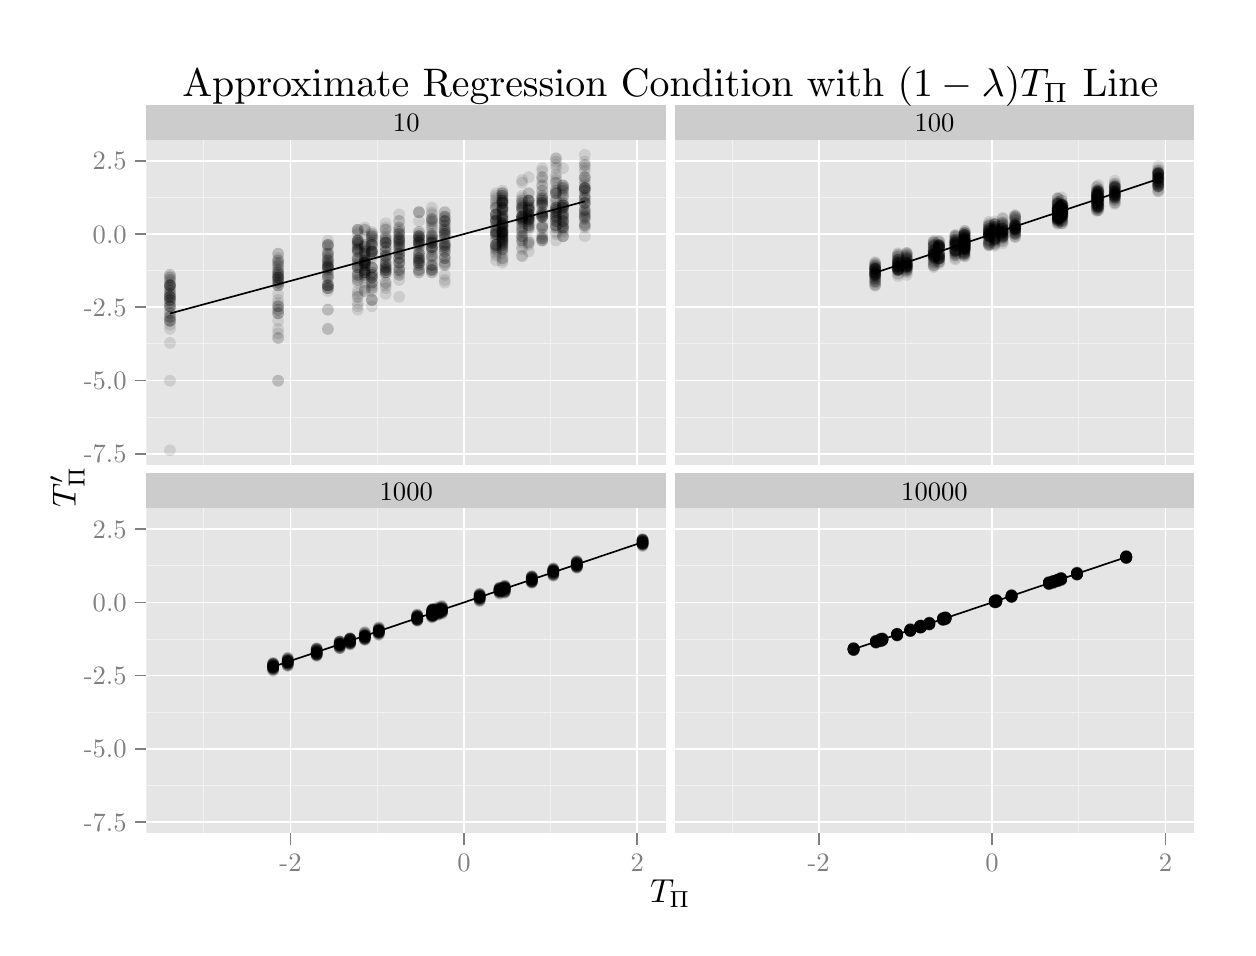
\begin{tikzpicture}[x=1pt,y=1pt]
\definecolor[named]{fillColor}{rgb}{1.00,1.00,1.00}
\path[use as bounding box,fill=fillColor,fill opacity=0.00] (0,0) rectangle (433.62,325.21);
\begin{scope}
\path[clip] (  0.00,  0.00) rectangle (433.62,325.21);
\definecolor[named]{drawColor}{rgb}{1.00,1.00,1.00}
\definecolor[named]{fillColor}{rgb}{1.00,1.00,1.00}

\path[draw=drawColor,line width= 0.6pt,line join=round,line cap=round,fill=fillColor] (  0.00,  0.00) rectangle (433.62,325.21);
\end{scope}
\begin{scope}
\path[clip] ( 42.89,167.14) rectangle (230.72,284.60);
\definecolor[named]{fillColor}{rgb}{0.90,0.90,0.90}

\path[fill=fillColor] ( 42.89,167.14) rectangle (230.72,284.60);
\definecolor[named]{drawColor}{rgb}{0.95,0.95,0.95}

\path[draw=drawColor,line width= 0.3pt,line join=round] ( 42.89,184.49) --
	(230.72,184.49);

\path[draw=drawColor,line width= 0.3pt,line join=round] ( 42.89,210.95) --
	(230.72,210.95);

\path[draw=drawColor,line width= 0.3pt,line join=round] ( 42.89,237.40) --
	(230.72,237.40);

\path[draw=drawColor,line width= 0.3pt,line join=round] ( 42.89,263.86) --
	(230.72,263.86);

\path[draw=drawColor,line width= 0.3pt,line join=round] ( 63.66,167.14) --
	( 63.66,284.60);

\path[draw=drawColor,line width= 0.3pt,line join=round] (126.31,167.14) --
	(126.31,284.60);

\path[draw=drawColor,line width= 0.3pt,line join=round] (188.96,167.14) --
	(188.96,284.60);
\definecolor[named]{drawColor}{rgb}{1.00,1.00,1.00}

\path[draw=drawColor,line width= 0.6pt,line join=round] ( 42.89,171.27) --
	(230.72,171.27);

\path[draw=drawColor,line width= 0.6pt,line join=round] ( 42.89,197.72) --
	(230.72,197.72);

\path[draw=drawColor,line width= 0.6pt,line join=round] ( 42.89,224.18) --
	(230.72,224.18);

\path[draw=drawColor,line width= 0.6pt,line join=round] ( 42.89,250.63) --
	(230.72,250.63);

\path[draw=drawColor,line width= 0.6pt,line join=round] ( 42.89,277.09) --
	(230.72,277.09);

\path[draw=drawColor,line width= 0.6pt,line join=round] ( 94.99,167.14) --
	( 94.99,284.60);

\path[draw=drawColor,line width= 0.6pt,line join=round] (157.64,167.14) --
	(157.64,284.60);

\path[draw=drawColor,line width= 0.6pt,line join=round] (220.29,167.14) --
	(220.29,284.60);
\definecolor[named]{fillColor}{rgb}{0.00,0.00,0.00}

\path[fill=fillColor,fill opacity=0.10] (201.31,256.92) circle (  2.13);

\path[fill=fillColor,fill opacity=0.10] (201.31,257.73) circle (  2.13);

\path[fill=fillColor,fill opacity=0.10] (201.31,259.36) circle (  2.13);

\path[fill=fillColor,fill opacity=0.10] (201.31,256.92) circle (  2.13);

\path[fill=fillColor,fill opacity=0.10] (201.31,261.87) circle (  2.13);

\path[fill=fillColor,fill opacity=0.10] (201.31,263.60) circle (  2.13);

\path[fill=fillColor,fill opacity=0.10] (201.31,268.19) circle (  2.13);

\path[fill=fillColor,fill opacity=0.10] (201.31,276.76) circle (  2.13);

\path[fill=fillColor,fill opacity=0.10] (201.31,271.18) circle (  2.13);

\path[fill=fillColor,fill opacity=0.10] (201.31,249.85) circle (  2.13);

\path[fill=fillColor,fill opacity=0.10] (201.31,252.97) circle (  2.13);

\path[fill=fillColor,fill opacity=0.10] (201.31,266.30) circle (  2.13);

\path[fill=fillColor,fill opacity=0.10] (201.31,258.54) circle (  2.13);

\path[fill=fillColor,fill opacity=0.10] (201.31,275.57) circle (  2.13);

\path[fill=fillColor,fill opacity=0.10] (201.31,266.30) circle (  2.13);

\path[fill=fillColor,fill opacity=0.10] (201.31,256.12) circle (  2.13);

\path[fill=fillColor,fill opacity=0.10] (201.31,267.23) circle (  2.13);

\path[fill=fillColor,fill opacity=0.10] (201.31,259.36) circle (  2.13);

\path[fill=fillColor,fill opacity=0.10] (201.31,279.26) circle (  2.13);

\path[fill=fillColor,fill opacity=0.10] (201.31,267.23) circle (  2.13);

\path[fill=fillColor,fill opacity=0.10] (201.31,266.30) circle (  2.13);

\path[fill=fillColor,fill opacity=0.10] (201.31,261.87) circle (  2.13);

\path[fill=fillColor,fill opacity=0.10] (201.31,262.73) circle (  2.13);

\path[fill=fillColor,fill opacity=0.10] (201.31,261.87) circle (  2.13);

\path[fill=fillColor,fill opacity=0.10] (201.31,258.54) circle (  2.13);

\path[fill=fillColor,fill opacity=0.10] (201.31,263.60) circle (  2.13);

\path[fill=fillColor,fill opacity=0.10] (201.31,264.48) circle (  2.13);

\path[fill=fillColor,fill opacity=0.10] (201.31,274.42) circle (  2.13);

\path[fill=fillColor,fill opacity=0.10] (201.31,267.23) circle (  2.13);

\path[fill=fillColor,fill opacity=0.10] (201.31,267.23) circle (  2.13);

\path[fill=fillColor,fill opacity=0.10] (201.31,264.48) circle (  2.13);

\path[fill=fillColor,fill opacity=0.10] (201.31,273.31) circle (  2.13);

\path[fill=fillColor,fill opacity=0.10] (201.31,253.75) circle (  2.13);

\path[fill=fillColor,fill opacity=0.10] (201.31,259.36) circle (  2.13);

\path[fill=fillColor,fill opacity=0.10] (201.31,271.18) circle (  2.13);

\path[fill=fillColor,fill opacity=0.10] (201.31,267.23) circle (  2.13);

\path[fill=fillColor,fill opacity=0.10] (201.31,271.18) circle (  2.13);

\path[fill=fillColor,fill opacity=0.10] (201.31,267.23) circle (  2.13);

\path[fill=fillColor,fill opacity=0.10] (201.31,257.73) circle (  2.13);

\path[fill=fillColor,fill opacity=0.10] (201.31,269.16) circle (  2.13);

\path[fill=fillColor,fill opacity=0.10] (201.31,253.75) circle (  2.13);

\path[fill=fillColor,fill opacity=0.10] (201.31,261.02) circle (  2.13);

\path[fill=fillColor,fill opacity=0.10] (201.31,261.87) circle (  2.13);

\path[fill=fillColor,fill opacity=0.10] (201.31,256.12) circle (  2.13);

\path[fill=fillColor,fill opacity=0.10] (201.31,263.60) circle (  2.13);

\path[fill=fillColor,fill opacity=0.10] (201.31,253.75) circle (  2.13);

\path[fill=fillColor,fill opacity=0.10] (201.31,270.16) circle (  2.13);

\path[fill=fillColor,fill opacity=0.10] (201.31,275.57) circle (  2.13);

\path[fill=fillColor,fill opacity=0.10] (201.31,254.54) circle (  2.13);

\path[fill=fillColor,fill opacity=0.10] (201.31,256.92) circle (  2.13);

\path[fill=fillColor,fill opacity=0.10] ( 51.42,227.95) circle (  2.13);

\path[fill=fillColor,fill opacity=0.10] ( 51.42,233.08) circle (  2.13);

\path[fill=fillColor,fill opacity=0.10] ( 51.42,220.68) circle (  2.13);

\path[fill=fillColor,fill opacity=0.10] ( 51.42,235.88) circle (  2.13);

\path[fill=fillColor,fill opacity=0.10] ( 51.42,234.96) circle (  2.13);

\path[fill=fillColor,fill opacity=0.10] ( 51.42,226.84) circle (  2.13);

\path[fill=fillColor,fill opacity=0.10] ( 51.42,230.08) circle (  2.13);

\path[fill=fillColor,fill opacity=0.10] ( 51.42,227.95) circle (  2.13);

\path[fill=fillColor,fill opacity=0.10] ( 51.42,226.84) circle (  2.13);

\path[fill=fillColor,fill opacity=0.10] ( 51.42,232.10) circle (  2.13);

\path[fill=fillColor,fill opacity=0.10] ( 51.42,231.10) circle (  2.13);

\path[fill=fillColor,fill opacity=0.10] ( 51.42,219.30) circle (  2.13);

\path[fill=fillColor,fill opacity=0.10] ( 51.42,211.29) circle (  2.13);

\path[fill=fillColor,fill opacity=0.10] ( 51.42,234.03) circle (  2.13);

\path[fill=fillColor,fill opacity=0.10] ( 51.42,232.10) circle (  2.13);

\path[fill=fillColor,fill opacity=0.10] ( 51.42,227.95) circle (  2.13);

\path[fill=fillColor,fill opacity=0.10] ( 51.42,234.96) circle (  2.13);

\path[fill=fillColor,fill opacity=0.10] ( 51.42,219.30) circle (  2.13);

\path[fill=fillColor,fill opacity=0.10] ( 51.42,232.10) circle (  2.13);

\path[fill=fillColor,fill opacity=0.10] ( 51.42,230.08) circle (  2.13);

\path[fill=fillColor,fill opacity=0.10] ( 51.42,227.95) circle (  2.13);

\path[fill=fillColor,fill opacity=0.10] ( 51.42,223.28) circle (  2.13);

\path[fill=fillColor,fill opacity=0.10] ( 51.42,222.01) circle (  2.13);

\path[fill=fillColor,fill opacity=0.10] ( 51.42,232.10) circle (  2.13);

\path[fill=fillColor,fill opacity=0.10] ( 51.42,232.10) circle (  2.13);

\path[fill=fillColor,fill opacity=0.10] ( 51.42,227.95) circle (  2.13);

\path[fill=fillColor,fill opacity=0.10] ( 51.42,224.51) circle (  2.13);

\path[fill=fillColor,fill opacity=0.10] ( 51.42,229.03) circle (  2.13);

\path[fill=fillColor,fill opacity=0.10] ( 51.42,217.86) circle (  2.13);

\path[fill=fillColor,fill opacity=0.10] ( 51.42,235.88) circle (  2.13);

\path[fill=fillColor,fill opacity=0.10] ( 51.42,234.03) circle (  2.13);

\path[fill=fillColor,fill opacity=0.10] ( 51.42,225.69) circle (  2.13);

\path[fill=fillColor,fill opacity=0.10] ( 51.42,172.48) circle (  2.13);

\path[fill=fillColor,fill opacity=0.10] ( 51.42,226.84) circle (  2.13);

\path[fill=fillColor,fill opacity=0.10] ( 51.42,224.51) circle (  2.13);

\path[fill=fillColor,fill opacity=0.10] ( 51.42,226.84) circle (  2.13);

\path[fill=fillColor,fill opacity=0.10] ( 51.42,219.30) circle (  2.13);

\path[fill=fillColor,fill opacity=0.10] ( 51.42,222.01) circle (  2.13);

\path[fill=fillColor,fill opacity=0.10] ( 51.42,224.51) circle (  2.13);

\path[fill=fillColor,fill opacity=0.10] ( 51.42,229.03) circle (  2.13);

\path[fill=fillColor,fill opacity=0.10] ( 51.42,224.51) circle (  2.13);

\path[fill=fillColor,fill opacity=0.10] ( 51.42,225.69) circle (  2.13);

\path[fill=fillColor,fill opacity=0.10] ( 51.42,231.10) circle (  2.13);

\path[fill=fillColor,fill opacity=0.10] ( 51.42,220.68) circle (  2.13);

\path[fill=fillColor,fill opacity=0.10] ( 51.42,216.34) circle (  2.13);

\path[fill=fillColor,fill opacity=0.10] ( 51.42,219.30) circle (  2.13);

\path[fill=fillColor,fill opacity=0.10] ( 51.42,232.10) circle (  2.13);

\path[fill=fillColor,fill opacity=0.10] ( 51.42,229.03) circle (  2.13);

\path[fill=fillColor,fill opacity=0.10] ( 51.42,197.63) circle (  2.13);

\path[fill=fillColor,fill opacity=0.10] ( 51.42,220.68) circle (  2.13);

\path[fill=fillColor,fill opacity=0.10] ( 90.50,232.10) circle (  2.13);

\path[fill=fillColor,fill opacity=0.10] ( 90.50,234.96) circle (  2.13);

\path[fill=fillColor,fill opacity=0.10] ( 90.50,239.39) circle (  2.13);

\path[fill=fillColor,fill opacity=0.10] ( 90.50,197.63) circle (  2.13);

\path[fill=fillColor,fill opacity=0.10] ( 90.50,241.08) circle (  2.13);

\path[fill=fillColor,fill opacity=0.10] ( 90.50,223.28) circle (  2.13);

\path[fill=fillColor,fill opacity=0.10] ( 90.50,235.88) circle (  2.13);

\path[fill=fillColor,fill opacity=0.10] ( 90.50,229.03) circle (  2.13);

\path[fill=fillColor,fill opacity=0.10] ( 90.50,234.03) circle (  2.13);

\path[fill=fillColor,fill opacity=0.10] ( 90.50,237.66) circle (  2.13);

\path[fill=fillColor,fill opacity=0.10] ( 90.50,222.01) circle (  2.13);

\path[fill=fillColor,fill opacity=0.10] ( 90.50,237.66) circle (  2.13);

\path[fill=fillColor,fill opacity=0.10] ( 90.50,213.07) circle (  2.13);

\path[fill=fillColor,fill opacity=0.10] ( 90.50,214.75) circle (  2.13);

\path[fill=fillColor,fill opacity=0.10] ( 90.50,236.78) circle (  2.13);

\path[fill=fillColor,fill opacity=0.10] ( 90.50,241.08) circle (  2.13);

\path[fill=fillColor,fill opacity=0.10] ( 90.50,240.24) circle (  2.13);

\path[fill=fillColor,fill opacity=0.10] ( 90.50,232.10) circle (  2.13);

\path[fill=fillColor,fill opacity=0.10] ( 90.50,232.10) circle (  2.13);

\path[fill=fillColor,fill opacity=0.10] ( 90.50,239.39) circle (  2.13);

\path[fill=fillColor,fill opacity=0.10] ( 90.50,241.91) circle (  2.13);

\path[fill=fillColor,fill opacity=0.10] ( 90.50,216.34) circle (  2.13);

\path[fill=fillColor,fill opacity=0.10] ( 90.50,224.51) circle (  2.13);

\path[fill=fillColor,fill opacity=0.10] ( 90.50,233.08) circle (  2.13);

\path[fill=fillColor,fill opacity=0.10] ( 90.50,236.78) circle (  2.13);

\path[fill=fillColor,fill opacity=0.10] ( 90.50,226.84) circle (  2.13);

\path[fill=fillColor,fill opacity=0.10] ( 90.50,235.88) circle (  2.13);

\path[fill=fillColor,fill opacity=0.10] ( 90.50,243.54) circle (  2.13);

\path[fill=fillColor,fill opacity=0.10] ( 90.50,243.54) circle (  2.13);

\path[fill=fillColor,fill opacity=0.10] ( 90.50,222.01) circle (  2.13);

\path[fill=fillColor,fill opacity=0.10] ( 90.50,197.63) circle (  2.13);

\path[fill=fillColor,fill opacity=0.10] ( 90.50,234.96) circle (  2.13);

\path[fill=fillColor,fill opacity=0.10] ( 90.50,233.08) circle (  2.13);

\path[fill=fillColor,fill opacity=0.10] ( 90.50,236.78) circle (  2.13);

\path[fill=fillColor,fill opacity=0.10] ( 90.50,223.28) circle (  2.13);

\path[fill=fillColor,fill opacity=0.10] ( 90.50,240.24) circle (  2.13);

\path[fill=fillColor,fill opacity=0.10] ( 90.50,234.96) circle (  2.13);

\path[fill=fillColor,fill opacity=0.10] ( 90.50,234.96) circle (  2.13);

\path[fill=fillColor,fill opacity=0.10] ( 90.50,219.30) circle (  2.13);

\path[fill=fillColor,fill opacity=0.10] ( 90.50,234.03) circle (  2.13);

\path[fill=fillColor,fill opacity=0.10] ( 90.50,233.08) circle (  2.13);

\path[fill=fillColor,fill opacity=0.10] ( 90.50,234.03) circle (  2.13);

\path[fill=fillColor,fill opacity=0.10] ( 90.50,235.88) circle (  2.13);

\path[fill=fillColor,fill opacity=0.10] ( 90.50,222.01) circle (  2.13);

\path[fill=fillColor,fill opacity=0.10] ( 90.50,225.69) circle (  2.13);

\path[fill=fillColor,fill opacity=0.10] ( 90.50,224.51) circle (  2.13);

\path[fill=fillColor,fill opacity=0.10] ( 90.50,213.07) circle (  2.13);

\path[fill=fillColor,fill opacity=0.10] ( 90.50,224.51) circle (  2.13);

\path[fill=fillColor,fill opacity=0.10] ( 90.50,238.54) circle (  2.13);

\path[fill=fillColor,fill opacity=0.10] ( 90.50,234.96) circle (  2.13);

\path[fill=fillColor,fill opacity=0.10] (181.04,262.73) circle (  2.13);

\path[fill=fillColor,fill opacity=0.10] (181.04,256.92) circle (  2.13);

\path[fill=fillColor,fill opacity=0.10] (181.04,256.12) circle (  2.13);

\path[fill=fillColor,fill opacity=0.10] (181.04,257.73) circle (  2.13);

\path[fill=fillColor,fill opacity=0.10] (181.04,255.33) circle (  2.13);

\path[fill=fillColor,fill opacity=0.10] (181.04,255.33) circle (  2.13);

\path[fill=fillColor,fill opacity=0.10] (181.04,261.02) circle (  2.13);

\path[fill=fillColor,fill opacity=0.10] (181.04,248.29) circle (  2.13);

\path[fill=fillColor,fill opacity=0.10] (181.04,256.92) circle (  2.13);

\path[fill=fillColor,fill opacity=0.10] (181.04,260.18) circle (  2.13);

\path[fill=fillColor,fill opacity=0.10] (181.04,271.18) circle (  2.13);

\path[fill=fillColor,fill opacity=0.10] (181.04,252.97) circle (  2.13);

\path[fill=fillColor,fill opacity=0.10] (181.04,256.12) circle (  2.13);

\path[fill=fillColor,fill opacity=0.10] (181.04,262.73) circle (  2.13);

\path[fill=fillColor,fill opacity=0.10] (181.04,265.38) circle (  2.13);

\path[fill=fillColor,fill opacity=0.10] (181.04,252.19) circle (  2.13);

\path[fill=fillColor,fill opacity=0.10] (181.04,257.73) circle (  2.13);

\path[fill=fillColor,fill opacity=0.10] (181.04,262.73) circle (  2.13);

\path[fill=fillColor,fill opacity=0.10] (181.04,244.34) circle (  2.13);

\path[fill=fillColor,fill opacity=0.10] (181.04,256.92) circle (  2.13);

\path[fill=fillColor,fill opacity=0.10] (181.04,262.73) circle (  2.13);

\path[fill=fillColor,fill opacity=0.10] (181.04,253.75) circle (  2.13);

\path[fill=fillColor,fill opacity=0.10] (181.04,256.12) circle (  2.13);

\path[fill=fillColor,fill opacity=0.10] (181.04,259.36) circle (  2.13);

\path[fill=fillColor,fill opacity=0.10] (181.04,256.92) circle (  2.13);

\path[fill=fillColor,fill opacity=0.10] (181.04,259.36) circle (  2.13);

\path[fill=fillColor,fill opacity=0.10] (181.04,261.87) circle (  2.13);

\path[fill=fillColor,fill opacity=0.10] (181.04,253.75) circle (  2.13);

\path[fill=fillColor,fill opacity=0.10] (181.04,257.73) circle (  2.13);

\path[fill=fillColor,fill opacity=0.10] (181.04,260.18) circle (  2.13);

\path[fill=fillColor,fill opacity=0.10] (181.04,265.38) circle (  2.13);

\path[fill=fillColor,fill opacity=0.10] (181.04,256.12) circle (  2.13);

\path[fill=fillColor,fill opacity=0.10] (181.04,253.75) circle (  2.13);

\path[fill=fillColor,fill opacity=0.10] (181.04,257.73) circle (  2.13);

\path[fill=fillColor,fill opacity=0.10] (181.04,255.33) circle (  2.13);

\path[fill=fillColor,fill opacity=0.10] (181.04,256.12) circle (  2.13);

\path[fill=fillColor,fill opacity=0.10] (181.04,262.73) circle (  2.13);

\path[fill=fillColor,fill opacity=0.10] (181.04,254.54) circle (  2.13);

\path[fill=fillColor,fill opacity=0.10] (181.04,252.97) circle (  2.13);

\path[fill=fillColor,fill opacity=0.10] (181.04,257.73) circle (  2.13);

\path[fill=fillColor,fill opacity=0.10] (181.04,259.36) circle (  2.13);

\path[fill=fillColor,fill opacity=0.10] (181.04,260.18) circle (  2.13);

\path[fill=fillColor,fill opacity=0.10] (181.04,247.51) circle (  2.13);

\path[fill=fillColor,fill opacity=0.10] (181.04,247.51) circle (  2.13);

\path[fill=fillColor,fill opacity=0.10] (181.04,259.36) circle (  2.13);

\path[fill=fillColor,fill opacity=0.10] (181.04,246.72) circle (  2.13);

\path[fill=fillColor,fill opacity=0.10] (181.04,260.18) circle (  2.13);

\path[fill=fillColor,fill opacity=0.10] (181.04,256.12) circle (  2.13);

\path[fill=fillColor,fill opacity=0.10] (181.04,259.36) circle (  2.13);

\path[fill=fillColor,fill opacity=0.10] (181.04,261.02) circle (  2.13);

\path[fill=fillColor,fill opacity=0.10] (190.90,257.73) circle (  2.13);

\path[fill=fillColor,fill opacity=0.10] (190.90,261.02) circle (  2.13);

\path[fill=fillColor,fill opacity=0.10] (190.90,265.38) circle (  2.13);

\path[fill=fillColor,fill opacity=0.10] (190.90,256.12) circle (  2.13);

\path[fill=fillColor,fill opacity=0.10] (190.90,251.41) circle (  2.13);

\path[fill=fillColor,fill opacity=0.10] (190.90,267.23) circle (  2.13);

\path[fill=fillColor,fill opacity=0.10] (190.90,265.38) circle (  2.13);

\path[fill=fillColor,fill opacity=0.10] (190.90,265.38) circle (  2.13);

\path[fill=fillColor,fill opacity=0.10] (190.90,252.97) circle (  2.13);

\path[fill=fillColor,fill opacity=0.10] (190.90,259.36) circle (  2.13);

\path[fill=fillColor,fill opacity=0.10] (190.90,272.23) circle (  2.13);

\path[fill=fillColor,fill opacity=0.10] (190.90,253.75) circle (  2.13);

\path[fill=fillColor,fill opacity=0.10] (190.90,256.92) circle (  2.13);

\path[fill=fillColor,fill opacity=0.10] (190.90,248.29) circle (  2.13);

\path[fill=fillColor,fill opacity=0.10] (190.90,262.73) circle (  2.13);

\path[fill=fillColor,fill opacity=0.10] (190.90,262.73) circle (  2.13);

\path[fill=fillColor,fill opacity=0.10] (190.90,258.54) circle (  2.13);

\path[fill=fillColor,fill opacity=0.10] (190.90,253.75) circle (  2.13);

\path[fill=fillColor,fill opacity=0.10] (190.90,276.76) circle (  2.13);

\path[fill=fillColor,fill opacity=0.10] (190.90,259.36) circle (  2.13);

\path[fill=fillColor,fill opacity=0.10] (190.90,255.33) circle (  2.13);

\path[fill=fillColor,fill opacity=0.10] (190.90,269.16) circle (  2.13);

\path[fill=fillColor,fill opacity=0.10] (190.90,258.54) circle (  2.13);

\path[fill=fillColor,fill opacity=0.10] (190.90,257.73) circle (  2.13);

\path[fill=fillColor,fill opacity=0.10] (190.90,260.18) circle (  2.13);

\path[fill=fillColor,fill opacity=0.10] (190.90,260.18) circle (  2.13);

\path[fill=fillColor,fill opacity=0.10] (190.90,260.18) circle (  2.13);

\path[fill=fillColor,fill opacity=0.10] (190.90,256.92) circle (  2.13);

\path[fill=fillColor,fill opacity=0.10] (190.90,252.97) circle (  2.13);

\path[fill=fillColor,fill opacity=0.10] (190.90,253.75) circle (  2.13);

\path[fill=fillColor,fill opacity=0.10] (190.90,266.30) circle (  2.13);

\path[fill=fillColor,fill opacity=0.10] (190.90,277.98) circle (  2.13);

\path[fill=fillColor,fill opacity=0.10] (190.90,269.16) circle (  2.13);

\path[fill=fillColor,fill opacity=0.10] (190.90,270.16) circle (  2.13);

\path[fill=fillColor,fill opacity=0.10] (190.90,274.42) circle (  2.13);

\path[fill=fillColor,fill opacity=0.10] (190.90,265.38) circle (  2.13);

\path[fill=fillColor,fill opacity=0.10] (190.90,255.33) circle (  2.13);

\path[fill=fillColor,fill opacity=0.10] (190.90,255.33) circle (  2.13);

\path[fill=fillColor,fill opacity=0.10] (190.90,260.18) circle (  2.13);

\path[fill=fillColor,fill opacity=0.10] (190.90,250.63) circle (  2.13);

\path[fill=fillColor,fill opacity=0.10] (190.90,263.60) circle (  2.13);

\path[fill=fillColor,fill opacity=0.10] (190.90,256.92) circle (  2.13);

\path[fill=fillColor,fill opacity=0.10] (190.90,258.54) circle (  2.13);

\path[fill=fillColor,fill opacity=0.10] (190.90,266.30) circle (  2.13);

\path[fill=fillColor,fill opacity=0.10] (190.90,277.98) circle (  2.13);

\path[fill=fillColor,fill opacity=0.10] (190.90,259.36) circle (  2.13);

\path[fill=fillColor,fill opacity=0.10] (190.90,256.92) circle (  2.13);

\path[fill=fillColor,fill opacity=0.10] (190.90,275.57) circle (  2.13);

\path[fill=fillColor,fill opacity=0.10] (190.90,271.18) circle (  2.13);

\path[fill=fillColor,fill opacity=0.10] (190.90,255.33) circle (  2.13);

\path[fill=fillColor,fill opacity=0.10] (171.54,252.97) circle (  2.13);

\path[fill=fillColor,fill opacity=0.10] (171.54,256.92) circle (  2.13);

\path[fill=fillColor,fill opacity=0.10] (171.54,264.48) circle (  2.13);

\path[fill=fillColor,fill opacity=0.10] (171.54,248.29) circle (  2.13);

\path[fill=fillColor,fill opacity=0.10] (171.54,248.29) circle (  2.13);

\path[fill=fillColor,fill opacity=0.10] (171.54,241.91) circle (  2.13);

\path[fill=fillColor,fill opacity=0.10] (171.54,257.73) circle (  2.13);

\path[fill=fillColor,fill opacity=0.10] (171.54,261.87) circle (  2.13);

\path[fill=fillColor,fill opacity=0.10] (171.54,241.91) circle (  2.13);

\path[fill=fillColor,fill opacity=0.10] (171.54,256.12) circle (  2.13);

\path[fill=fillColor,fill opacity=0.10] (171.54,260.18) circle (  2.13);

\path[fill=fillColor,fill opacity=0.10] (171.54,250.63) circle (  2.13);

\path[fill=fillColor,fill opacity=0.10] (171.54,250.63) circle (  2.13);

\path[fill=fillColor,fill opacity=0.10] (171.54,259.36) circle (  2.13);

\path[fill=fillColor,fill opacity=0.10] (171.54,254.54) circle (  2.13);

\path[fill=fillColor,fill opacity=0.10] (171.54,252.97) circle (  2.13);

\path[fill=fillColor,fill opacity=0.10] (171.54,256.92) circle (  2.13);

\path[fill=fillColor,fill opacity=0.10] (171.54,253.75) circle (  2.13);

\path[fill=fillColor,fill opacity=0.10] (171.54,251.41) circle (  2.13);

\path[fill=fillColor,fill opacity=0.10] (171.54,256.12) circle (  2.13);

\path[fill=fillColor,fill opacity=0.10] (171.54,254.54) circle (  2.13);

\path[fill=fillColor,fill opacity=0.10] (171.54,251.41) circle (  2.13);

\path[fill=fillColor,fill opacity=0.10] (171.54,250.63) circle (  2.13);

\path[fill=fillColor,fill opacity=0.10] (171.54,260.18) circle (  2.13);

\path[fill=fillColor,fill opacity=0.10] (171.54,265.38) circle (  2.13);

\path[fill=fillColor,fill opacity=0.10] (171.54,247.51) circle (  2.13);

\path[fill=fillColor,fill opacity=0.10] (171.54,240.24) circle (  2.13);

\path[fill=fillColor,fill opacity=0.10] (171.54,251.41) circle (  2.13);

\path[fill=fillColor,fill opacity=0.10] (171.54,266.30) circle (  2.13);

\path[fill=fillColor,fill opacity=0.10] (171.54,262.73) circle (  2.13);

\path[fill=fillColor,fill opacity=0.10] (171.54,259.36) circle (  2.13);

\path[fill=fillColor,fill opacity=0.10] (171.54,249.07) circle (  2.13);

\path[fill=fillColor,fill opacity=0.10] (171.54,259.36) circle (  2.13);

\path[fill=fillColor,fill opacity=0.10] (171.54,251.41) circle (  2.13);

\path[fill=fillColor,fill opacity=0.10] (171.54,252.19) circle (  2.13);

\path[fill=fillColor,fill opacity=0.10] (171.54,249.85) circle (  2.13);

\path[fill=fillColor,fill opacity=0.10] (171.54,250.63) circle (  2.13);

\path[fill=fillColor,fill opacity=0.10] (171.54,260.18) circle (  2.13);

\path[fill=fillColor,fill opacity=0.10] (171.54,245.14) circle (  2.13);

\path[fill=fillColor,fill opacity=0.10] (171.54,249.07) circle (  2.13);

\path[fill=fillColor,fill opacity=0.10] (171.54,259.36) circle (  2.13);

\path[fill=fillColor,fill opacity=0.10] (171.54,252.19) circle (  2.13);

\path[fill=fillColor,fill opacity=0.10] (171.54,262.73) circle (  2.13);

\path[fill=fillColor,fill opacity=0.10] (171.54,251.41) circle (  2.13);

\path[fill=fillColor,fill opacity=0.10] (171.54,253.75) circle (  2.13);

\path[fill=fillColor,fill opacity=0.10] (171.54,262.73) circle (  2.13);

\path[fill=fillColor,fill opacity=0.10] (171.54,263.60) circle (  2.13);

\path[fill=fillColor,fill opacity=0.10] (171.54,246.72) circle (  2.13);

\path[fill=fillColor,fill opacity=0.10] (171.54,256.12) circle (  2.13);

\path[fill=fillColor,fill opacity=0.10] (171.54,252.97) circle (  2.13);

\path[fill=fillColor,fill opacity=0.10] (169.21,257.73) circle (  2.13);

\path[fill=fillColor,fill opacity=0.10] (169.21,245.14) circle (  2.13);

\path[fill=fillColor,fill opacity=0.10] (169.21,257.73) circle (  2.13);

\path[fill=fillColor,fill opacity=0.10] (169.21,260.18) circle (  2.13);

\path[fill=fillColor,fill opacity=0.10] (169.21,251.41) circle (  2.13);

\path[fill=fillColor,fill opacity=0.10] (169.21,251.41) circle (  2.13);

\path[fill=fillColor,fill opacity=0.10] (169.21,249.07) circle (  2.13);

\path[fill=fillColor,fill opacity=0.10] (169.21,257.73) circle (  2.13);

\path[fill=fillColor,fill opacity=0.10] (169.21,250.63) circle (  2.13);

\path[fill=fillColor,fill opacity=0.10] (169.21,245.14) circle (  2.13);

\path[fill=fillColor,fill opacity=0.10] (169.21,246.72) circle (  2.13);

\path[fill=fillColor,fill opacity=0.10] (169.21,255.33) circle (  2.13);

\path[fill=fillColor,fill opacity=0.10] (169.21,261.02) circle (  2.13);

\path[fill=fillColor,fill opacity=0.10] (169.21,242.73) circle (  2.13);

\path[fill=fillColor,fill opacity=0.10] (169.21,250.63) circle (  2.13);

\path[fill=fillColor,fill opacity=0.10] (169.21,257.73) circle (  2.13);

\path[fill=fillColor,fill opacity=0.10] (169.21,262.73) circle (  2.13);

\path[fill=fillColor,fill opacity=0.10] (169.21,256.12) circle (  2.13);

\path[fill=fillColor,fill opacity=0.10] (169.21,257.73) circle (  2.13);

\path[fill=fillColor,fill opacity=0.10] (169.21,251.41) circle (  2.13);

\path[fill=fillColor,fill opacity=0.10] (169.21,250.63) circle (  2.13);

\path[fill=fillColor,fill opacity=0.10] (169.21,256.12) circle (  2.13);

\path[fill=fillColor,fill opacity=0.10] (169.21,265.38) circle (  2.13);

\path[fill=fillColor,fill opacity=0.10] (169.21,250.63) circle (  2.13);

\path[fill=fillColor,fill opacity=0.10] (169.21,255.33) circle (  2.13);

\path[fill=fillColor,fill opacity=0.10] (169.21,252.97) circle (  2.13);

\path[fill=fillColor,fill opacity=0.10] (169.21,246.72) circle (  2.13);

\path[fill=fillColor,fill opacity=0.10] (169.21,244.34) circle (  2.13);

\path[fill=fillColor,fill opacity=0.10] (169.21,248.29) circle (  2.13);

\path[fill=fillColor,fill opacity=0.10] (169.21,263.60) circle (  2.13);

\path[fill=fillColor,fill opacity=0.10] (169.21,246.72) circle (  2.13);

\path[fill=fillColor,fill opacity=0.10] (169.21,246.72) circle (  2.13);

\path[fill=fillColor,fill opacity=0.10] (169.21,245.93) circle (  2.13);

\path[fill=fillColor,fill opacity=0.10] (169.21,264.48) circle (  2.13);

\path[fill=fillColor,fill opacity=0.10] (169.21,260.18) circle (  2.13);

\path[fill=fillColor,fill opacity=0.10] (169.21,256.92) circle (  2.13);

\path[fill=fillColor,fill opacity=0.10] (169.21,261.87) circle (  2.13);

\path[fill=fillColor,fill opacity=0.10] (169.21,253.75) circle (  2.13);

\path[fill=fillColor,fill opacity=0.10] (169.21,255.33) circle (  2.13);

\path[fill=fillColor,fill opacity=0.10] (169.21,251.41) circle (  2.13);

\path[fill=fillColor,fill opacity=0.10] (169.21,255.33) circle (  2.13);

\path[fill=fillColor,fill opacity=0.10] (169.21,246.72) circle (  2.13);

\path[fill=fillColor,fill opacity=0.10] (169.21,245.93) circle (  2.13);

\path[fill=fillColor,fill opacity=0.10] (169.21,253.75) circle (  2.13);

\path[fill=fillColor,fill opacity=0.10] (169.21,260.18) circle (  2.13);

\path[fill=fillColor,fill opacity=0.10] (169.21,249.85) circle (  2.13);

\path[fill=fillColor,fill opacity=0.10] (169.21,255.33) circle (  2.13);

\path[fill=fillColor,fill opacity=0.10] (169.21,243.54) circle (  2.13);

\path[fill=fillColor,fill opacity=0.10] (169.21,241.08) circle (  2.13);

\path[fill=fillColor,fill opacity=0.10] (169.21,252.19) circle (  2.13);

\path[fill=fillColor,fill opacity=0.10] (121.83,231.10) circle (  2.13);

\path[fill=fillColor,fill opacity=0.10] (121.83,241.91) circle (  2.13);

\path[fill=fillColor,fill opacity=0.10] (121.83,240.24) circle (  2.13);

\path[fill=fillColor,fill opacity=0.10] (121.83,236.78) circle (  2.13);

\path[fill=fillColor,fill opacity=0.10] (121.83,240.24) circle (  2.13);

\path[fill=fillColor,fill opacity=0.10] (121.83,240.24) circle (  2.13);

\path[fill=fillColor,fill opacity=0.10] (121.83,234.96) circle (  2.13);

\path[fill=fillColor,fill opacity=0.10] (121.83,243.54) circle (  2.13);

\path[fill=fillColor,fill opacity=0.10] (121.83,237.66) circle (  2.13);

\path[fill=fillColor,fill opacity=0.10] (121.83,235.88) circle (  2.13);

\path[fill=fillColor,fill opacity=0.10] (121.83,245.14) circle (  2.13);

\path[fill=fillColor,fill opacity=0.10] (121.83,239.39) circle (  2.13);

\path[fill=fillColor,fill opacity=0.10] (121.83,245.93) circle (  2.13);

\path[fill=fillColor,fill opacity=0.10] (121.83,241.08) circle (  2.13);

\path[fill=fillColor,fill opacity=0.10] (121.83,237.66) circle (  2.13);

\path[fill=fillColor,fill opacity=0.10] (121.83,236.78) circle (  2.13);

\path[fill=fillColor,fill opacity=0.10] (121.83,252.19) circle (  2.13);

\path[fill=fillColor,fill opacity=0.10] (121.83,245.93) circle (  2.13);

\path[fill=fillColor,fill opacity=0.10] (121.83,239.39) circle (  2.13);

\path[fill=fillColor,fill opacity=0.10] (121.83,236.78) circle (  2.13);

\path[fill=fillColor,fill opacity=0.10] (121.83,235.88) circle (  2.13);

\path[fill=fillColor,fill opacity=0.10] (121.83,245.93) circle (  2.13);

\path[fill=fillColor,fill opacity=0.10] (121.83,240.24) circle (  2.13);

\path[fill=fillColor,fill opacity=0.10] (121.83,242.73) circle (  2.13);

\path[fill=fillColor,fill opacity=0.10] (121.83,236.78) circle (  2.13);

\path[fill=fillColor,fill opacity=0.10] (121.83,237.66) circle (  2.13);

\path[fill=fillColor,fill opacity=0.10] (121.83,241.08) circle (  2.13);

\path[fill=fillColor,fill opacity=0.10] (121.83,239.39) circle (  2.13);

\path[fill=fillColor,fill opacity=0.10] (121.83,241.08) circle (  2.13);

\path[fill=fillColor,fill opacity=0.10] (121.83,236.78) circle (  2.13);

\path[fill=fillColor,fill opacity=0.10] (121.83,240.24) circle (  2.13);

\path[fill=fillColor,fill opacity=0.10] (121.83,230.08) circle (  2.13);

\path[fill=fillColor,fill opacity=0.10] (121.83,252.19) circle (  2.13);

\path[fill=fillColor,fill opacity=0.10] (121.83,246.72) circle (  2.13);

\path[fill=fillColor,fill opacity=0.10] (121.83,240.24) circle (  2.13);

\path[fill=fillColor,fill opacity=0.10] (121.83,230.08) circle (  2.13);

\path[fill=fillColor,fill opacity=0.10] (121.83,240.24) circle (  2.13);

\path[fill=fillColor,fill opacity=0.10] (121.83,244.34) circle (  2.13);

\path[fill=fillColor,fill opacity=0.10] (121.83,246.72) circle (  2.13);

\path[fill=fillColor,fill opacity=0.10] (121.83,241.08) circle (  2.13);

\path[fill=fillColor,fill opacity=0.10] (121.83,244.34) circle (  2.13);

\path[fill=fillColor,fill opacity=0.10] (121.83,233.08) circle (  2.13);

\path[fill=fillColor,fill opacity=0.10] (121.83,239.39) circle (  2.13);

\path[fill=fillColor,fill opacity=0.10] (121.83,235.88) circle (  2.13);

\path[fill=fillColor,fill opacity=0.10] (121.83,241.91) circle (  2.13);

\path[fill=fillColor,fill opacity=0.10] (121.83,249.85) circle (  2.13);

\path[fill=fillColor,fill opacity=0.10] (121.83,240.24) circle (  2.13);

\path[fill=fillColor,fill opacity=0.10] (121.83,252.97) circle (  2.13);

\path[fill=fillColor,fill opacity=0.10] (121.83,243.54) circle (  2.13);

\path[fill=fillColor,fill opacity=0.10] (121.83,244.34) circle (  2.13);

\path[fill=fillColor,fill opacity=0.10] (171.54,258.54) circle (  2.13);

\path[fill=fillColor,fill opacity=0.10] (171.54,244.34) circle (  2.13);

\path[fill=fillColor,fill opacity=0.10] (171.54,265.38) circle (  2.13);

\path[fill=fillColor,fill opacity=0.10] (171.54,245.14) circle (  2.13);

\path[fill=fillColor,fill opacity=0.10] (171.54,246.72) circle (  2.13);

\path[fill=fillColor,fill opacity=0.10] (171.54,247.51) circle (  2.13);

\path[fill=fillColor,fill opacity=0.10] (171.54,260.18) circle (  2.13);

\path[fill=fillColor,fill opacity=0.10] (171.54,249.85) circle (  2.13);

\path[fill=fillColor,fill opacity=0.10] (171.54,263.60) circle (  2.13);

\path[fill=fillColor,fill opacity=0.10] (171.54,243.54) circle (  2.13);

\path[fill=fillColor,fill opacity=0.10] (171.54,249.07) circle (  2.13);

\path[fill=fillColor,fill opacity=0.10] (171.54,248.29) circle (  2.13);

\path[fill=fillColor,fill opacity=0.10] (171.54,246.72) circle (  2.13);

\path[fill=fillColor,fill opacity=0.10] (171.54,245.93) circle (  2.13);

\path[fill=fillColor,fill opacity=0.10] (171.54,261.87) circle (  2.13);

\path[fill=fillColor,fill opacity=0.10] (171.54,245.14) circle (  2.13);

\path[fill=fillColor,fill opacity=0.10] (171.54,248.29) circle (  2.13);

\path[fill=fillColor,fill opacity=0.10] (171.54,251.41) circle (  2.13);

\path[fill=fillColor,fill opacity=0.10] (171.54,254.54) circle (  2.13);

\path[fill=fillColor,fill opacity=0.10] (171.54,251.41) circle (  2.13);

\path[fill=fillColor,fill opacity=0.10] (171.54,249.85) circle (  2.13);

\path[fill=fillColor,fill opacity=0.10] (171.54,261.87) circle (  2.13);

\path[fill=fillColor,fill opacity=0.10] (171.54,254.54) circle (  2.13);

\path[fill=fillColor,fill opacity=0.10] (171.54,256.92) circle (  2.13);

\path[fill=fillColor,fill opacity=0.10] (171.54,257.73) circle (  2.13);

\path[fill=fillColor,fill opacity=0.10] (171.54,249.85) circle (  2.13);

\path[fill=fillColor,fill opacity=0.10] (171.54,256.12) circle (  2.13);

\path[fill=fillColor,fill opacity=0.10] (171.54,247.51) circle (  2.13);

\path[fill=fillColor,fill opacity=0.10] (171.54,260.18) circle (  2.13);

\path[fill=fillColor,fill opacity=0.10] (171.54,253.75) circle (  2.13);

\path[fill=fillColor,fill opacity=0.10] (171.54,247.51) circle (  2.13);

\path[fill=fillColor,fill opacity=0.10] (171.54,245.93) circle (  2.13);

\path[fill=fillColor,fill opacity=0.10] (171.54,264.48) circle (  2.13);

\path[fill=fillColor,fill opacity=0.10] (171.54,265.38) circle (  2.13);

\path[fill=fillColor,fill opacity=0.10] (171.54,241.08) circle (  2.13);

\path[fill=fillColor,fill opacity=0.10] (171.54,262.73) circle (  2.13);

\path[fill=fillColor,fill opacity=0.10] (171.54,253.75) circle (  2.13);

\path[fill=fillColor,fill opacity=0.10] (171.54,250.63) circle (  2.13);

\path[fill=fillColor,fill opacity=0.10] (171.54,261.87) circle (  2.13);

\path[fill=fillColor,fill opacity=0.10] (171.54,253.75) circle (  2.13);

\path[fill=fillColor,fill opacity=0.10] (171.54,254.54) circle (  2.13);

\path[fill=fillColor,fill opacity=0.10] (171.54,262.73) circle (  2.13);

\path[fill=fillColor,fill opacity=0.10] (171.54,256.12) circle (  2.13);

\path[fill=fillColor,fill opacity=0.10] (171.54,249.07) circle (  2.13);

\path[fill=fillColor,fill opacity=0.10] (171.54,253.75) circle (  2.13);

\path[fill=fillColor,fill opacity=0.10] (171.54,249.07) circle (  2.13);

\path[fill=fillColor,fill opacity=0.10] (171.54,261.87) circle (  2.13);

\path[fill=fillColor,fill opacity=0.10] (171.54,264.48) circle (  2.13);

\path[fill=fillColor,fill opacity=0.10] (171.54,252.19) circle (  2.13);

\path[fill=fillColor,fill opacity=0.10] (171.54,261.87) circle (  2.13);

\path[fill=fillColor,fill opacity=0.10] (119.26,250.63) circle (  2.13);

\path[fill=fillColor,fill opacity=0.10] (119.26,248.29) circle (  2.13);

\path[fill=fillColor,fill opacity=0.10] (119.26,235.88) circle (  2.13);

\path[fill=fillColor,fill opacity=0.10] (119.26,244.34) circle (  2.13);

\path[fill=fillColor,fill opacity=0.10] (119.26,247.51) circle (  2.13);

\path[fill=fillColor,fill opacity=0.10] (119.26,227.95) circle (  2.13);

\path[fill=fillColor,fill opacity=0.10] (119.26,252.19) circle (  2.13);

\path[fill=fillColor,fill opacity=0.10] (119.26,248.29) circle (  2.13);

\path[fill=fillColor,fill opacity=0.10] (119.26,245.93) circle (  2.13);

\path[fill=fillColor,fill opacity=0.10] (119.26,241.08) circle (  2.13);

\path[fill=fillColor,fill opacity=0.10] (119.26,238.54) circle (  2.13);

\path[fill=fillColor,fill opacity=0.10] (119.26,223.28) circle (  2.13);

\path[fill=fillColor,fill opacity=0.10] (119.26,245.14) circle (  2.13);

\path[fill=fillColor,fill opacity=0.10] (119.26,244.34) circle (  2.13);

\path[fill=fillColor,fill opacity=0.10] (119.26,252.19) circle (  2.13);

\path[fill=fillColor,fill opacity=0.10] (119.26,241.91) circle (  2.13);

\path[fill=fillColor,fill opacity=0.10] (119.26,240.24) circle (  2.13);

\path[fill=fillColor,fill opacity=0.10] (119.26,244.34) circle (  2.13);

\path[fill=fillColor,fill opacity=0.10] (119.26,245.14) circle (  2.13);

\path[fill=fillColor,fill opacity=0.10] (119.26,241.08) circle (  2.13);

\path[fill=fillColor,fill opacity=0.10] (119.26,248.29) circle (  2.13);

\path[fill=fillColor,fill opacity=0.10] (119.26,252.19) circle (  2.13);

\path[fill=fillColor,fill opacity=0.10] (119.26,245.14) circle (  2.13);

\path[fill=fillColor,fill opacity=0.10] (119.26,234.03) circle (  2.13);

\path[fill=fillColor,fill opacity=0.10] (119.26,247.51) circle (  2.13);

\path[fill=fillColor,fill opacity=0.10] (119.26,233.08) circle (  2.13);

\path[fill=fillColor,fill opacity=0.10] (119.26,248.29) circle (  2.13);

\path[fill=fillColor,fill opacity=0.10] (119.26,225.69) circle (  2.13);

\path[fill=fillColor,fill opacity=0.10] (119.26,238.54) circle (  2.13);

\path[fill=fillColor,fill opacity=0.10] (119.26,236.78) circle (  2.13);

\path[fill=fillColor,fill opacity=0.10] (119.26,239.39) circle (  2.13);

\path[fill=fillColor,fill opacity=0.10] (119.26,246.72) circle (  2.13);

\path[fill=fillColor,fill opacity=0.10] (119.26,241.91) circle (  2.13);

\path[fill=fillColor,fill opacity=0.10] (119.26,241.91) circle (  2.13);

\path[fill=fillColor,fill opacity=0.10] (119.26,246.72) circle (  2.13);

\path[fill=fillColor,fill opacity=0.10] (119.26,234.03) circle (  2.13);

\path[fill=fillColor,fill opacity=0.10] (119.26,230.08) circle (  2.13);

\path[fill=fillColor,fill opacity=0.10] (119.26,227.95) circle (  2.13);

\path[fill=fillColor,fill opacity=0.10] (119.26,247.51) circle (  2.13);

\path[fill=fillColor,fill opacity=0.10] (119.26,239.39) circle (  2.13);

\path[fill=fillColor,fill opacity=0.10] (119.26,251.41) circle (  2.13);

\path[fill=fillColor,fill opacity=0.10] (119.26,245.14) circle (  2.13);

\path[fill=fillColor,fill opacity=0.10] (119.26,224.51) circle (  2.13);

\path[fill=fillColor,fill opacity=0.10] (119.26,238.54) circle (  2.13);

\path[fill=fillColor,fill opacity=0.10] (119.26,235.88) circle (  2.13);

\path[fill=fillColor,fill opacity=0.10] (119.26,229.03) circle (  2.13);

\path[fill=fillColor,fill opacity=0.10] (119.26,234.96) circle (  2.13);

\path[fill=fillColor,fill opacity=0.10] (119.26,248.29) circle (  2.13);

\path[fill=fillColor,fill opacity=0.10] (119.26,238.54) circle (  2.13);

\path[fill=fillColor,fill opacity=0.10] (119.26,235.88) circle (  2.13);

\path[fill=fillColor,fill opacity=0.10] (178.64,256.92) circle (  2.13);

\path[fill=fillColor,fill opacity=0.10] (178.64,249.85) circle (  2.13);

\path[fill=fillColor,fill opacity=0.10] (178.64,249.85) circle (  2.13);

\path[fill=fillColor,fill opacity=0.10] (178.64,260.18) circle (  2.13);

\path[fill=fillColor,fill opacity=0.10] (178.64,256.92) circle (  2.13);

\path[fill=fillColor,fill opacity=0.10] (178.64,261.02) circle (  2.13);

\path[fill=fillColor,fill opacity=0.10] (178.64,261.87) circle (  2.13);

\path[fill=fillColor,fill opacity=0.10] (178.64,245.14) circle (  2.13);

\path[fill=fillColor,fill opacity=0.10] (178.64,255.33) circle (  2.13);

\path[fill=fillColor,fill opacity=0.10] (178.64,256.92) circle (  2.13);

\path[fill=fillColor,fill opacity=0.10] (178.64,252.97) circle (  2.13);

\path[fill=fillColor,fill opacity=0.10] (178.64,259.36) circle (  2.13);

\path[fill=fillColor,fill opacity=0.10] (178.64,245.93) circle (  2.13);

\path[fill=fillColor,fill opacity=0.10] (178.64,258.54) circle (  2.13);

\path[fill=fillColor,fill opacity=0.10] (178.64,264.48) circle (  2.13);

\path[fill=fillColor,fill opacity=0.10] (178.64,253.75) circle (  2.13);

\path[fill=fillColor,fill opacity=0.10] (178.64,256.92) circle (  2.13);

\path[fill=fillColor,fill opacity=0.10] (178.64,256.12) circle (  2.13);

\path[fill=fillColor,fill opacity=0.10] (178.64,242.73) circle (  2.13);

\path[fill=fillColor,fill opacity=0.10] (178.64,252.97) circle (  2.13);

\path[fill=fillColor,fill opacity=0.10] (178.64,248.29) circle (  2.13);

\path[fill=fillColor,fill opacity=0.10] (178.64,261.02) circle (  2.13);

\path[fill=fillColor,fill opacity=0.10] (178.64,242.73) circle (  2.13);

\path[fill=fillColor,fill opacity=0.10] (178.64,256.12) circle (  2.13);

\path[fill=fillColor,fill opacity=0.10] (178.64,247.51) circle (  2.13);

\path[fill=fillColor,fill opacity=0.10] (178.64,263.60) circle (  2.13);

\path[fill=fillColor,fill opacity=0.10] (178.64,269.16) circle (  2.13);

\path[fill=fillColor,fill opacity=0.10] (178.64,254.54) circle (  2.13);

\path[fill=fillColor,fill opacity=0.10] (178.64,260.18) circle (  2.13);

\path[fill=fillColor,fill opacity=0.10] (178.64,270.16) circle (  2.13);

\path[fill=fillColor,fill opacity=0.10] (178.64,251.41) circle (  2.13);

\path[fill=fillColor,fill opacity=0.10] (178.64,255.33) circle (  2.13);

\path[fill=fillColor,fill opacity=0.10] (178.64,256.92) circle (  2.13);

\path[fill=fillColor,fill opacity=0.10] (178.64,260.18) circle (  2.13);

\path[fill=fillColor,fill opacity=0.10] (178.64,256.92) circle (  2.13);

\path[fill=fillColor,fill opacity=0.10] (178.64,262.73) circle (  2.13);

\path[fill=fillColor,fill opacity=0.10] (178.64,259.36) circle (  2.13);

\path[fill=fillColor,fill opacity=0.10] (178.64,260.18) circle (  2.13);

\path[fill=fillColor,fill opacity=0.10] (178.64,256.12) circle (  2.13);

\path[fill=fillColor,fill opacity=0.10] (178.64,249.07) circle (  2.13);

\path[fill=fillColor,fill opacity=0.10] (178.64,252.19) circle (  2.13);

\path[fill=fillColor,fill opacity=0.10] (178.64,261.87) circle (  2.13);

\path[fill=fillColor,fill opacity=0.10] (178.64,256.12) circle (  2.13);

\path[fill=fillColor,fill opacity=0.10] (178.64,248.29) circle (  2.13);

\path[fill=fillColor,fill opacity=0.10] (178.64,256.12) circle (  2.13);

\path[fill=fillColor,fill opacity=0.10] (178.64,256.92) circle (  2.13);

\path[fill=fillColor,fill opacity=0.10] (178.64,262.73) circle (  2.13);

\path[fill=fillColor,fill opacity=0.10] (178.64,249.85) circle (  2.13);

\path[fill=fillColor,fill opacity=0.10] (178.64,255.33) circle (  2.13);

\path[fill=fillColor,fill opacity=0.10] (178.64,251.41) circle (  2.13);

\path[fill=fillColor,fill opacity=0.10] (124.38,244.34) circle (  2.13);

\path[fill=fillColor,fill opacity=0.10] (124.38,226.84) circle (  2.13);

\path[fill=fillColor,fill opacity=0.10] (124.38,246.72) circle (  2.13);

\path[fill=fillColor,fill opacity=0.10] (124.38,234.96) circle (  2.13);

\path[fill=fillColor,fill opacity=0.10] (124.38,249.85) circle (  2.13);

\path[fill=fillColor,fill opacity=0.10] (124.38,233.08) circle (  2.13);

\path[fill=fillColor,fill opacity=0.10] (124.38,234.96) circle (  2.13);

\path[fill=fillColor,fill opacity=0.10] (124.38,245.14) circle (  2.13);

\path[fill=fillColor,fill opacity=0.10] (124.38,241.91) circle (  2.13);

\path[fill=fillColor,fill opacity=0.10] (124.38,243.54) circle (  2.13);

\path[fill=fillColor,fill opacity=0.10] (124.38,250.63) circle (  2.13);

\path[fill=fillColor,fill opacity=0.10] (124.38,236.78) circle (  2.13);

\path[fill=fillColor,fill opacity=0.10] (124.38,250.63) circle (  2.13);

\path[fill=fillColor,fill opacity=0.10] (124.38,246.72) circle (  2.13);

\path[fill=fillColor,fill opacity=0.10] (124.38,247.51) circle (  2.13);

\path[fill=fillColor,fill opacity=0.10] (124.38,244.34) circle (  2.13);

\path[fill=fillColor,fill opacity=0.10] (124.38,235.88) circle (  2.13);

\path[fill=fillColor,fill opacity=0.10] (124.38,249.85) circle (  2.13);

\path[fill=fillColor,fill opacity=0.10] (124.38,238.54) circle (  2.13);

\path[fill=fillColor,fill opacity=0.10] (124.38,231.10) circle (  2.13);

\path[fill=fillColor,fill opacity=0.10] (124.38,233.08) circle (  2.13);

\path[fill=fillColor,fill opacity=0.10] (124.38,236.78) circle (  2.13);

\path[fill=fillColor,fill opacity=0.10] (124.38,231.10) circle (  2.13);

\path[fill=fillColor,fill opacity=0.10] (124.38,251.41) circle (  2.13);

\path[fill=fillColor,fill opacity=0.10] (124.38,232.10) circle (  2.13);

\path[fill=fillColor,fill opacity=0.10] (124.38,249.07) circle (  2.13);

\path[fill=fillColor,fill opacity=0.10] (124.38,244.34) circle (  2.13);

\path[fill=fillColor,fill opacity=0.10] (124.38,235.88) circle (  2.13);

\path[fill=fillColor,fill opacity=0.10] (124.38,249.85) circle (  2.13);

\path[fill=fillColor,fill opacity=0.10] (124.38,238.54) circle (  2.13);

\path[fill=fillColor,fill opacity=0.10] (124.38,246.72) circle (  2.13);

\path[fill=fillColor,fill opacity=0.10] (124.38,235.88) circle (  2.13);

\path[fill=fillColor,fill opacity=0.10] (124.38,249.07) circle (  2.13);

\path[fill=fillColor,fill opacity=0.10] (124.38,248.29) circle (  2.13);

\path[fill=fillColor,fill opacity=0.10] (124.38,238.54) circle (  2.13);

\path[fill=fillColor,fill opacity=0.10] (124.38,244.34) circle (  2.13);

\path[fill=fillColor,fill opacity=0.10] (124.38,247.51) circle (  2.13);

\path[fill=fillColor,fill opacity=0.10] (124.38,244.34) circle (  2.13);

\path[fill=fillColor,fill opacity=0.10] (124.38,243.54) circle (  2.13);

\path[fill=fillColor,fill opacity=0.10] (124.38,224.51) circle (  2.13);

\path[fill=fillColor,fill opacity=0.10] (124.38,242.73) circle (  2.13);

\path[fill=fillColor,fill opacity=0.10] (124.38,230.08) circle (  2.13);

\path[fill=fillColor,fill opacity=0.10] (124.38,238.54) circle (  2.13);

\path[fill=fillColor,fill opacity=0.10] (124.38,246.72) circle (  2.13);

\path[fill=fillColor,fill opacity=0.10] (124.38,234.96) circle (  2.13);

\path[fill=fillColor,fill opacity=0.10] (124.38,226.84) circle (  2.13);

\path[fill=fillColor,fill opacity=0.10] (124.38,233.08) circle (  2.13);

\path[fill=fillColor,fill opacity=0.10] (124.38,244.34) circle (  2.13);

\path[fill=fillColor,fill opacity=0.10] (124.38,234.96) circle (  2.13);

\path[fill=fillColor,fill opacity=0.10] (124.38,226.84) circle (  2.13);

\path[fill=fillColor,fill opacity=0.10] (129.36,248.29) circle (  2.13);

\path[fill=fillColor,fill opacity=0.10] (129.36,249.07) circle (  2.13);

\path[fill=fillColor,fill opacity=0.10] (129.36,238.54) circle (  2.13);

\path[fill=fillColor,fill opacity=0.10] (129.36,249.85) circle (  2.13);

\path[fill=fillColor,fill opacity=0.10] (129.36,238.54) circle (  2.13);

\path[fill=fillColor,fill opacity=0.10] (129.36,244.34) circle (  2.13);

\path[fill=fillColor,fill opacity=0.10] (129.36,237.66) circle (  2.13);

\path[fill=fillColor,fill opacity=0.10] (129.36,235.88) circle (  2.13);

\path[fill=fillColor,fill opacity=0.10] (129.36,239.39) circle (  2.13);

\path[fill=fillColor,fill opacity=0.10] (129.36,242.73) circle (  2.13);

\path[fill=fillColor,fill opacity=0.10] (129.36,245.93) circle (  2.13);

\path[fill=fillColor,fill opacity=0.10] (129.36,233.08) circle (  2.13);

\path[fill=fillColor,fill opacity=0.10] (129.36,252.19) circle (  2.13);

\path[fill=fillColor,fill opacity=0.10] (129.36,238.54) circle (  2.13);

\path[fill=fillColor,fill opacity=0.10] (129.36,229.03) circle (  2.13);

\path[fill=fillColor,fill opacity=0.10] (129.36,247.51) circle (  2.13);

\path[fill=fillColor,fill opacity=0.10] (129.36,236.78) circle (  2.13);

\path[fill=fillColor,fill opacity=0.10] (129.36,242.73) circle (  2.13);

\path[fill=fillColor,fill opacity=0.10] (129.36,239.39) circle (  2.13);

\path[fill=fillColor,fill opacity=0.10] (129.36,245.93) circle (  2.13);

\path[fill=fillColor,fill opacity=0.10] (129.36,247.51) circle (  2.13);

\path[fill=fillColor,fill opacity=0.10] (129.36,242.73) circle (  2.13);

\path[fill=fillColor,fill opacity=0.10] (129.36,232.10) circle (  2.13);

\path[fill=fillColor,fill opacity=0.10] (129.36,244.34) circle (  2.13);

\path[fill=fillColor,fill opacity=0.10] (129.36,247.51) circle (  2.13);

\path[fill=fillColor,fill opacity=0.10] (129.36,237.66) circle (  2.13);

\path[fill=fillColor,fill opacity=0.10] (129.36,247.51) circle (  2.13);

\path[fill=fillColor,fill opacity=0.10] (129.36,245.93) circle (  2.13);

\path[fill=fillColor,fill opacity=0.10] (129.36,236.78) circle (  2.13);

\path[fill=fillColor,fill opacity=0.10] (129.36,250.63) circle (  2.13);

\path[fill=fillColor,fill opacity=0.10] (129.36,249.07) circle (  2.13);

\path[fill=fillColor,fill opacity=0.10] (129.36,237.66) circle (  2.13);

\path[fill=fillColor,fill opacity=0.10] (129.36,254.54) circle (  2.13);

\path[fill=fillColor,fill opacity=0.10] (129.36,240.24) circle (  2.13);

\path[fill=fillColor,fill opacity=0.10] (129.36,252.97) circle (  2.13);

\path[fill=fillColor,fill opacity=0.10] (129.36,248.29) circle (  2.13);

\path[fill=fillColor,fill opacity=0.10] (129.36,237.66) circle (  2.13);

\path[fill=fillColor,fill opacity=0.10] (129.36,240.24) circle (  2.13);

\path[fill=fillColor,fill opacity=0.10] (129.36,231.10) circle (  2.13);

\path[fill=fillColor,fill opacity=0.10] (129.36,252.19) circle (  2.13);

\path[fill=fillColor,fill opacity=0.10] (129.36,238.54) circle (  2.13);

\path[fill=fillColor,fill opacity=0.10] (129.36,233.08) circle (  2.13);

\path[fill=fillColor,fill opacity=0.10] (129.36,244.34) circle (  2.13);

\path[fill=fillColor,fill opacity=0.10] (129.36,241.91) circle (  2.13);

\path[fill=fillColor,fill opacity=0.10] (129.36,247.51) circle (  2.13);

\path[fill=fillColor,fill opacity=0.10] (129.36,241.91) circle (  2.13);

\path[fill=fillColor,fill opacity=0.10] (129.36,242.73) circle (  2.13);

\path[fill=fillColor,fill opacity=0.10] (129.36,236.78) circle (  2.13);

\path[fill=fillColor,fill opacity=0.10] (129.36,240.24) circle (  2.13);

\path[fill=fillColor,fill opacity=0.10] (129.36,236.78) circle (  2.13);

\path[fill=fillColor,fill opacity=0.10] (150.72,245.93) circle (  2.13);

\path[fill=fillColor,fill opacity=0.10] (150.72,250.63) circle (  2.13);

\path[fill=fillColor,fill opacity=0.10] (150.72,255.33) circle (  2.13);

\path[fill=fillColor,fill opacity=0.10] (150.72,249.07) circle (  2.13);

\path[fill=fillColor,fill opacity=0.10] (150.72,250.63) circle (  2.13);

\path[fill=fillColor,fill opacity=0.10] (150.72,245.93) circle (  2.13);

\path[fill=fillColor,fill opacity=0.10] (150.72,244.34) circle (  2.13);

\path[fill=fillColor,fill opacity=0.10] (150.72,255.33) circle (  2.13);

\path[fill=fillColor,fill opacity=0.10] (150.72,235.88) circle (  2.13);

\path[fill=fillColor,fill opacity=0.10] (150.72,250.63) circle (  2.13);

\path[fill=fillColor,fill opacity=0.10] (150.72,252.97) circle (  2.13);

\path[fill=fillColor,fill opacity=0.10] (150.72,253.75) circle (  2.13);

\path[fill=fillColor,fill opacity=0.10] (150.72,247.51) circle (  2.13);

\path[fill=fillColor,fill opacity=0.10] (150.72,245.14) circle (  2.13);

\path[fill=fillColor,fill opacity=0.10] (150.72,233.08) circle (  2.13);

\path[fill=fillColor,fill opacity=0.10] (150.72,256.92) circle (  2.13);

\path[fill=fillColor,fill opacity=0.10] (150.72,255.33) circle (  2.13);

\path[fill=fillColor,fill opacity=0.10] (150.72,239.39) circle (  2.13);

\path[fill=fillColor,fill opacity=0.10] (150.72,249.85) circle (  2.13);

\path[fill=fillColor,fill opacity=0.10] (150.72,255.33) circle (  2.13);

\path[fill=fillColor,fill opacity=0.10] (150.72,247.51) circle (  2.13);

\path[fill=fillColor,fill opacity=0.10] (150.72,246.72) circle (  2.13);

\path[fill=fillColor,fill opacity=0.10] (150.72,246.72) circle (  2.13);

\path[fill=fillColor,fill opacity=0.10] (150.72,241.91) circle (  2.13);

\path[fill=fillColor,fill opacity=0.10] (150.72,256.12) circle (  2.13);

\path[fill=fillColor,fill opacity=0.10] (150.72,252.19) circle (  2.13);

\path[fill=fillColor,fill opacity=0.10] (150.72,234.03) circle (  2.13);

\path[fill=fillColor,fill opacity=0.10] (150.72,241.91) circle (  2.13);

\path[fill=fillColor,fill opacity=0.10] (150.72,254.54) circle (  2.13);

\path[fill=fillColor,fill opacity=0.10] (150.72,251.41) circle (  2.13);

\path[fill=fillColor,fill opacity=0.10] (150.72,258.54) circle (  2.13);

\path[fill=fillColor,fill opacity=0.10] (150.72,252.19) circle (  2.13);

\path[fill=fillColor,fill opacity=0.10] (150.72,250.63) circle (  2.13);

\path[fill=fillColor,fill opacity=0.10] (150.72,240.24) circle (  2.13);

\path[fill=fillColor,fill opacity=0.10] (150.72,239.39) circle (  2.13);

\path[fill=fillColor,fill opacity=0.10] (150.72,241.91) circle (  2.13);

\path[fill=fillColor,fill opacity=0.10] (150.72,246.72) circle (  2.13);

\path[fill=fillColor,fill opacity=0.10] (150.72,244.34) circle (  2.13);

\path[fill=fillColor,fill opacity=0.10] (150.72,258.54) circle (  2.13);

\path[fill=fillColor,fill opacity=0.10] (150.72,251.41) circle (  2.13);

\path[fill=fillColor,fill opacity=0.10] (150.72,256.92) circle (  2.13);

\path[fill=fillColor,fill opacity=0.10] (150.72,256.92) circle (  2.13);

\path[fill=fillColor,fill opacity=0.10] (150.72,246.72) circle (  2.13);

\path[fill=fillColor,fill opacity=0.10] (150.72,244.34) circle (  2.13);

\path[fill=fillColor,fill opacity=0.10] (150.72,242.73) circle (  2.13);

\path[fill=fillColor,fill opacity=0.10] (150.72,249.07) circle (  2.13);

\path[fill=fillColor,fill opacity=0.10] (150.72,245.93) circle (  2.13);

\path[fill=fillColor,fill opacity=0.10] (150.72,240.24) circle (  2.13);

\path[fill=fillColor,fill opacity=0.10] (150.72,253.75) circle (  2.13);

\path[fill=fillColor,fill opacity=0.10] (150.72,252.19) circle (  2.13);

\path[fill=fillColor,fill opacity=0.10] (193.44,255.33) circle (  2.13);

\path[fill=fillColor,fill opacity=0.10] (193.44,260.18) circle (  2.13);

\path[fill=fillColor,fill opacity=0.10] (193.44,257.73) circle (  2.13);

\path[fill=fillColor,fill opacity=0.10] (193.44,263.60) circle (  2.13);

\path[fill=fillColor,fill opacity=0.10] (193.44,256.92) circle (  2.13);

\path[fill=fillColor,fill opacity=0.10] (193.44,261.02) circle (  2.13);

\path[fill=fillColor,fill opacity=0.10] (193.44,261.02) circle (  2.13);

\path[fill=fillColor,fill opacity=0.10] (193.44,255.33) circle (  2.13);

\path[fill=fillColor,fill opacity=0.10] (193.44,267.23) circle (  2.13);

\path[fill=fillColor,fill opacity=0.10] (193.44,260.18) circle (  2.13);

\path[fill=fillColor,fill opacity=0.10] (193.44,257.73) circle (  2.13);

\path[fill=fillColor,fill opacity=0.10] (193.44,253.75) circle (  2.13);

\path[fill=fillColor,fill opacity=0.10] (193.44,261.02) circle (  2.13);

\path[fill=fillColor,fill opacity=0.10] (193.44,252.97) circle (  2.13);

\path[fill=fillColor,fill opacity=0.10] (193.44,255.33) circle (  2.13);

\path[fill=fillColor,fill opacity=0.10] (193.44,256.12) circle (  2.13);

\path[fill=fillColor,fill opacity=0.10] (193.44,260.18) circle (  2.13);

\path[fill=fillColor,fill opacity=0.10] (193.44,252.97) circle (  2.13);

\path[fill=fillColor,fill opacity=0.10] (193.44,261.02) circle (  2.13);

\path[fill=fillColor,fill opacity=0.10] (193.44,266.30) circle (  2.13);

\path[fill=fillColor,fill opacity=0.10] (193.44,256.92) circle (  2.13);

\path[fill=fillColor,fill opacity=0.10] (193.44,252.97) circle (  2.13);

\path[fill=fillColor,fill opacity=0.10] (193.44,264.48) circle (  2.13);

\path[fill=fillColor,fill opacity=0.10] (193.44,253.75) circle (  2.13);

\path[fill=fillColor,fill opacity=0.10] (193.44,252.19) circle (  2.13);

\path[fill=fillColor,fill opacity=0.10] (193.44,265.38) circle (  2.13);

\path[fill=fillColor,fill opacity=0.10] (193.44,274.42) circle (  2.13);

\path[fill=fillColor,fill opacity=0.10] (193.44,261.87) circle (  2.13);

\path[fill=fillColor,fill opacity=0.10] (193.44,252.97) circle (  2.13);

\path[fill=fillColor,fill opacity=0.10] (193.44,251.41) circle (  2.13);

\path[fill=fillColor,fill opacity=0.10] (193.44,249.85) circle (  2.13);

\path[fill=fillColor,fill opacity=0.10] (193.44,268.19) circle (  2.13);

\path[fill=fillColor,fill opacity=0.10] (193.44,260.18) circle (  2.13);

\path[fill=fillColor,fill opacity=0.10] (193.44,257.73) circle (  2.13);

\path[fill=fillColor,fill opacity=0.10] (193.44,267.23) circle (  2.13);

\path[fill=fillColor,fill opacity=0.10] (193.44,264.48) circle (  2.13);

\path[fill=fillColor,fill opacity=0.10] (193.44,268.19) circle (  2.13);

\path[fill=fillColor,fill opacity=0.10] (193.44,259.36) circle (  2.13);

\path[fill=fillColor,fill opacity=0.10] (193.44,261.02) circle (  2.13);

\path[fill=fillColor,fill opacity=0.10] (193.44,260.18) circle (  2.13);

\path[fill=fillColor,fill opacity=0.10] (193.44,249.85) circle (  2.13);

\path[fill=fillColor,fill opacity=0.10] (193.44,256.92) circle (  2.13);

\path[fill=fillColor,fill opacity=0.10] (193.44,249.85) circle (  2.13);

\path[fill=fillColor,fill opacity=0.10] (193.44,258.54) circle (  2.13);

\path[fill=fillColor,fill opacity=0.10] (193.44,268.19) circle (  2.13);

\path[fill=fillColor,fill opacity=0.10] (193.44,254.54) circle (  2.13);

\path[fill=fillColor,fill opacity=0.10] (193.44,255.33) circle (  2.13);

\path[fill=fillColor,fill opacity=0.10] (193.44,266.30) circle (  2.13);

\path[fill=fillColor,fill opacity=0.10] (193.44,267.23) circle (  2.13);

\path[fill=fillColor,fill opacity=0.10] (193.44,261.87) circle (  2.13);

\path[fill=fillColor,fill opacity=0.10] (108.49,246.72) circle (  2.13);

\path[fill=fillColor,fill opacity=0.10] (108.49,230.08) circle (  2.13);

\path[fill=fillColor,fill opacity=0.10] (108.49,241.08) circle (  2.13);

\path[fill=fillColor,fill opacity=0.10] (108.49,231.10) circle (  2.13);

\path[fill=fillColor,fill opacity=0.10] (108.49,241.91) circle (  2.13);

\path[fill=fillColor,fill opacity=0.10] (108.49,243.54) circle (  2.13);

\path[fill=fillColor,fill opacity=0.10] (108.49,239.39) circle (  2.13);

\path[fill=fillColor,fill opacity=0.10] (108.49,232.10) circle (  2.13);

\path[fill=fillColor,fill opacity=0.10] (108.49,231.10) circle (  2.13);

\path[fill=fillColor,fill opacity=0.10] (108.49,244.34) circle (  2.13);

\path[fill=fillColor,fill opacity=0.10] (108.49,246.72) circle (  2.13);

\path[fill=fillColor,fill opacity=0.10] (108.49,245.93) circle (  2.13);

\path[fill=fillColor,fill opacity=0.10] (108.49,231.10) circle (  2.13);

\path[fill=fillColor,fill opacity=0.10] (108.49,238.54) circle (  2.13);

\path[fill=fillColor,fill opacity=0.10] (108.49,238.54) circle (  2.13);

\path[fill=fillColor,fill opacity=0.10] (108.49,241.08) circle (  2.13);

\path[fill=fillColor,fill opacity=0.10] (108.49,235.88) circle (  2.13);

\path[fill=fillColor,fill opacity=0.10] (108.49,223.28) circle (  2.13);

\path[fill=fillColor,fill opacity=0.10] (108.49,240.24) circle (  2.13);

\path[fill=fillColor,fill opacity=0.10] (108.49,235.88) circle (  2.13);

\path[fill=fillColor,fill opacity=0.10] (108.49,238.54) circle (  2.13);

\path[fill=fillColor,fill opacity=0.10] (108.49,216.34) circle (  2.13);

\path[fill=fillColor,fill opacity=0.10] (108.49,232.10) circle (  2.13);

\path[fill=fillColor,fill opacity=0.10] (108.49,241.08) circle (  2.13);

\path[fill=fillColor,fill opacity=0.10] (108.49,238.54) circle (  2.13);

\path[fill=fillColor,fill opacity=0.10] (108.49,223.28) circle (  2.13);

\path[fill=fillColor,fill opacity=0.10] (108.49,239.39) circle (  2.13);

\path[fill=fillColor,fill opacity=0.10] (108.49,234.96) circle (  2.13);

\path[fill=fillColor,fill opacity=0.10] (108.49,231.10) circle (  2.13);

\path[fill=fillColor,fill opacity=0.10] (108.49,242.73) circle (  2.13);

\path[fill=fillColor,fill opacity=0.10] (108.49,241.91) circle (  2.13);

\path[fill=fillColor,fill opacity=0.10] (108.49,232.10) circle (  2.13);

\path[fill=fillColor,fill opacity=0.10] (108.49,243.54) circle (  2.13);

\path[fill=fillColor,fill opacity=0.10] (108.49,236.78) circle (  2.13);

\path[fill=fillColor,fill opacity=0.10] (108.49,237.66) circle (  2.13);

\path[fill=fillColor,fill opacity=0.10] (108.49,232.10) circle (  2.13);

\path[fill=fillColor,fill opacity=0.10] (108.49,237.66) circle (  2.13);

\path[fill=fillColor,fill opacity=0.10] (108.49,240.24) circle (  2.13);

\path[fill=fillColor,fill opacity=0.10] (108.49,239.39) circle (  2.13);

\path[fill=fillColor,fill opacity=0.10] (108.49,239.39) circle (  2.13);

\path[fill=fillColor,fill opacity=0.10] (108.49,246.72) circle (  2.13);

\path[fill=fillColor,fill opacity=0.10] (108.49,248.29) circle (  2.13);

\path[fill=fillColor,fill opacity=0.10] (108.49,243.54) circle (  2.13);

\path[fill=fillColor,fill opacity=0.10] (108.49,216.34) circle (  2.13);

\path[fill=fillColor,fill opacity=0.10] (108.49,246.72) circle (  2.13);

\path[fill=fillColor,fill opacity=0.10] (108.49,234.96) circle (  2.13);

\path[fill=fillColor,fill opacity=0.10] (108.49,232.10) circle (  2.13);

\path[fill=fillColor,fill opacity=0.10] (108.49,234.96) circle (  2.13);

\path[fill=fillColor,fill opacity=0.10] (108.49,233.08) circle (  2.13);

\path[fill=fillColor,fill opacity=0.10] (108.49,238.54) circle (  2.13);

\path[fill=fillColor,fill opacity=0.10] (141.39,241.08) circle (  2.13);

\path[fill=fillColor,fill opacity=0.10] (141.39,245.93) circle (  2.13);

\path[fill=fillColor,fill opacity=0.10] (141.39,241.91) circle (  2.13);

\path[fill=fillColor,fill opacity=0.10] (141.39,236.78) circle (  2.13);

\path[fill=fillColor,fill opacity=0.10] (141.39,250.63) circle (  2.13);

\path[fill=fillColor,fill opacity=0.10] (141.39,239.39) circle (  2.13);

\path[fill=fillColor,fill opacity=0.10] (141.39,241.91) circle (  2.13);

\path[fill=fillColor,fill opacity=0.10] (141.39,247.51) circle (  2.13);

\path[fill=fillColor,fill opacity=0.10] (141.39,248.29) circle (  2.13);

\path[fill=fillColor,fill opacity=0.10] (141.39,243.54) circle (  2.13);

\path[fill=fillColor,fill opacity=0.10] (141.39,242.73) circle (  2.13);

\path[fill=fillColor,fill opacity=0.10] (141.39,241.08) circle (  2.13);

\path[fill=fillColor,fill opacity=0.10] (141.39,241.91) circle (  2.13);

\path[fill=fillColor,fill opacity=0.10] (141.39,249.85) circle (  2.13);

\path[fill=fillColor,fill opacity=0.10] (141.39,237.66) circle (  2.13);

\path[fill=fillColor,fill opacity=0.10] (141.39,247.51) circle (  2.13);

\path[fill=fillColor,fill opacity=0.10] (141.39,251.41) circle (  2.13);

\path[fill=fillColor,fill opacity=0.10] (141.39,244.34) circle (  2.13);

\path[fill=fillColor,fill opacity=0.10] (141.39,243.54) circle (  2.13);

\path[fill=fillColor,fill opacity=0.10] (141.39,258.54) circle (  2.13);

\path[fill=fillColor,fill opacity=0.10] (141.39,258.54) circle (  2.13);

\path[fill=fillColor,fill opacity=0.10] (141.39,237.66) circle (  2.13);

\path[fill=fillColor,fill opacity=0.10] (141.39,246.72) circle (  2.13);

\path[fill=fillColor,fill opacity=0.10] (141.39,240.24) circle (  2.13);

\path[fill=fillColor,fill opacity=0.10] (141.39,249.85) circle (  2.13);

\path[fill=fillColor,fill opacity=0.10] (141.39,249.85) circle (  2.13);

\path[fill=fillColor,fill opacity=0.10] (141.39,258.54) circle (  2.13);

\path[fill=fillColor,fill opacity=0.10] (141.39,248.29) circle (  2.13);

\path[fill=fillColor,fill opacity=0.10] (141.39,249.07) circle (  2.13);

\path[fill=fillColor,fill opacity=0.10] (141.39,247.51) circle (  2.13);

\path[fill=fillColor,fill opacity=0.10] (141.39,255.33) circle (  2.13);

\path[fill=fillColor,fill opacity=0.10] (141.39,249.07) circle (  2.13);

\path[fill=fillColor,fill opacity=0.10] (141.39,251.41) circle (  2.13);

\path[fill=fillColor,fill opacity=0.10] (141.39,241.08) circle (  2.13);

\path[fill=fillColor,fill opacity=0.10] (141.39,245.93) circle (  2.13);

\path[fill=fillColor,fill opacity=0.10] (141.39,248.29) circle (  2.13);

\path[fill=fillColor,fill opacity=0.10] (141.39,237.66) circle (  2.13);

\path[fill=fillColor,fill opacity=0.10] (141.39,247.51) circle (  2.13);

\path[fill=fillColor,fill opacity=0.10] (141.39,241.91) circle (  2.13);

\path[fill=fillColor,fill opacity=0.10] (141.39,243.54) circle (  2.13);

\path[fill=fillColor,fill opacity=0.10] (141.39,246.72) circle (  2.13);

\path[fill=fillColor,fill opacity=0.10] (141.39,249.85) circle (  2.13);

\path[fill=fillColor,fill opacity=0.10] (141.39,240.24) circle (  2.13);

\path[fill=fillColor,fill opacity=0.10] (141.39,240.24) circle (  2.13);

\path[fill=fillColor,fill opacity=0.10] (141.39,239.39) circle (  2.13);

\path[fill=fillColor,fill opacity=0.10] (141.39,240.24) circle (  2.13);

\path[fill=fillColor,fill opacity=0.10] (141.39,249.07) circle (  2.13);

\path[fill=fillColor,fill opacity=0.10] (141.39,249.85) circle (  2.13);

\path[fill=fillColor,fill opacity=0.10] (141.39,247.51) circle (  2.13);

\path[fill=fillColor,fill opacity=0.10] (141.39,236.78) circle (  2.13);

\path[fill=fillColor,fill opacity=0.10] (134.24,248.29) circle (  2.13);

\path[fill=fillColor,fill opacity=0.10] (134.24,251.41) circle (  2.13);

\path[fill=fillColor,fill opacity=0.10] (134.24,245.14) circle (  2.13);

\path[fill=fillColor,fill opacity=0.10] (134.24,241.91) circle (  2.13);

\path[fill=fillColor,fill opacity=0.10] (134.24,252.19) circle (  2.13);

\path[fill=fillColor,fill opacity=0.10] (134.24,234.03) circle (  2.13);

\path[fill=fillColor,fill opacity=0.10] (134.24,252.97) circle (  2.13);

\path[fill=fillColor,fill opacity=0.10] (134.24,249.07) circle (  2.13);

\path[fill=fillColor,fill opacity=0.10] (134.24,252.97) circle (  2.13);

\path[fill=fillColor,fill opacity=0.10] (134.24,241.91) circle (  2.13);

\path[fill=fillColor,fill opacity=0.10] (134.24,243.54) circle (  2.13);

\path[fill=fillColor,fill opacity=0.10] (134.24,255.33) circle (  2.13);

\path[fill=fillColor,fill opacity=0.10] (134.24,246.72) circle (  2.13);

\path[fill=fillColor,fill opacity=0.10] (134.24,246.72) circle (  2.13);

\path[fill=fillColor,fill opacity=0.10] (134.24,249.85) circle (  2.13);

\path[fill=fillColor,fill opacity=0.10] (134.24,250.63) circle (  2.13);

\path[fill=fillColor,fill opacity=0.10] (134.24,246.72) circle (  2.13);

\path[fill=fillColor,fill opacity=0.10] (134.24,255.33) circle (  2.13);

\path[fill=fillColor,fill opacity=0.10] (134.24,248.29) circle (  2.13);

\path[fill=fillColor,fill opacity=0.10] (134.24,238.54) circle (  2.13);

\path[fill=fillColor,fill opacity=0.10] (134.24,247.51) circle (  2.13);

\path[fill=fillColor,fill opacity=0.10] (134.24,249.07) circle (  2.13);

\path[fill=fillColor,fill opacity=0.10] (134.24,237.66) circle (  2.13);

\path[fill=fillColor,fill opacity=0.10] (134.24,227.95) circle (  2.13);

\path[fill=fillColor,fill opacity=0.10] (134.24,244.34) circle (  2.13);

\path[fill=fillColor,fill opacity=0.10] (134.24,247.51) circle (  2.13);

\path[fill=fillColor,fill opacity=0.10] (134.24,245.93) circle (  2.13);

\path[fill=fillColor,fill opacity=0.10] (134.24,240.24) circle (  2.13);

\path[fill=fillColor,fill opacity=0.10] (134.24,249.07) circle (  2.13);

\path[fill=fillColor,fill opacity=0.10] (134.24,236.78) circle (  2.13);

\path[fill=fillColor,fill opacity=0.10] (134.24,250.63) circle (  2.13);

\path[fill=fillColor,fill opacity=0.10] (134.24,235.88) circle (  2.13);

\path[fill=fillColor,fill opacity=0.10] (134.24,243.54) circle (  2.13);

\path[fill=fillColor,fill opacity=0.10] (134.24,251.41) circle (  2.13);

\path[fill=fillColor,fill opacity=0.10] (134.24,240.24) circle (  2.13);

\path[fill=fillColor,fill opacity=0.10] (134.24,243.54) circle (  2.13);

\path[fill=fillColor,fill opacity=0.10] (134.24,257.73) circle (  2.13);

\path[fill=fillColor,fill opacity=0.10] (134.24,243.54) circle (  2.13);

\path[fill=fillColor,fill opacity=0.10] (134.24,245.93) circle (  2.13);

\path[fill=fillColor,fill opacity=0.10] (134.24,250.63) circle (  2.13);

\path[fill=fillColor,fill opacity=0.10] (134.24,237.66) circle (  2.13);

\path[fill=fillColor,fill opacity=0.10] (134.24,245.14) circle (  2.13);

\path[fill=fillColor,fill opacity=0.10] (134.24,235.88) circle (  2.13);

\path[fill=fillColor,fill opacity=0.10] (134.24,240.24) circle (  2.13);

\path[fill=fillColor,fill opacity=0.10] (134.24,248.29) circle (  2.13);

\path[fill=fillColor,fill opacity=0.10] (134.24,237.66) circle (  2.13);

\path[fill=fillColor,fill opacity=0.10] (134.24,241.91) circle (  2.13);

\path[fill=fillColor,fill opacity=0.10] (134.24,248.29) circle (  2.13);

\path[fill=fillColor,fill opacity=0.10] (134.24,240.24) circle (  2.13);

\path[fill=fillColor,fill opacity=0.10] (134.24,241.91) circle (  2.13);

\path[fill=fillColor,fill opacity=0.10] (185.92,256.92) circle (  2.13);

\path[fill=fillColor,fill opacity=0.10] (185.92,256.92) circle (  2.13);

\path[fill=fillColor,fill opacity=0.10] (185.92,261.02) circle (  2.13);

\path[fill=fillColor,fill opacity=0.10] (185.92,249.07) circle (  2.13);

\path[fill=fillColor,fill opacity=0.10] (185.92,262.73) circle (  2.13);

\path[fill=fillColor,fill opacity=0.10] (185.92,261.87) circle (  2.13);

\path[fill=fillColor,fill opacity=0.10] (185.92,257.73) circle (  2.13);

\path[fill=fillColor,fill opacity=0.10] (185.92,250.63) circle (  2.13);

\path[fill=fillColor,fill opacity=0.10] (185.92,258.54) circle (  2.13);

\path[fill=fillColor,fill opacity=0.10] (185.92,273.31) circle (  2.13);

\path[fill=fillColor,fill opacity=0.10] (185.92,253.75) circle (  2.13);

\path[fill=fillColor,fill opacity=0.10] (185.92,248.29) circle (  2.13);

\path[fill=fillColor,fill opacity=0.10] (185.92,268.19) circle (  2.13);

\path[fill=fillColor,fill opacity=0.10] (185.92,257.73) circle (  2.13);

\path[fill=fillColor,fill opacity=0.10] (185.92,257.73) circle (  2.13);

\path[fill=fillColor,fill opacity=0.10] (185.92,249.07) circle (  2.13);

\path[fill=fillColor,fill opacity=0.10] (185.92,271.18) circle (  2.13);

\path[fill=fillColor,fill opacity=0.10] (185.92,252.97) circle (  2.13);

\path[fill=fillColor,fill opacity=0.10] (185.92,249.85) circle (  2.13);

\path[fill=fillColor,fill opacity=0.10] (185.92,271.18) circle (  2.13);

\path[fill=fillColor,fill opacity=0.10] (185.92,256.92) circle (  2.13);

\path[fill=fillColor,fill opacity=0.10] (185.92,262.73) circle (  2.13);

\path[fill=fillColor,fill opacity=0.10] (185.92,274.42) circle (  2.13);

\path[fill=fillColor,fill opacity=0.10] (185.92,252.97) circle (  2.13);

\path[fill=fillColor,fill opacity=0.10] (185.92,256.92) circle (  2.13);

\path[fill=fillColor,fill opacity=0.10] (185.92,257.73) circle (  2.13);

\path[fill=fillColor,fill opacity=0.10] (185.92,252.97) circle (  2.13);

\path[fill=fillColor,fill opacity=0.10] (185.92,248.29) circle (  2.13);

\path[fill=fillColor,fill opacity=0.10] (185.92,256.92) circle (  2.13);

\path[fill=fillColor,fill opacity=0.10] (185.92,266.30) circle (  2.13);

\path[fill=fillColor,fill opacity=0.10] (185.92,266.30) circle (  2.13);

\path[fill=fillColor,fill opacity=0.10] (185.92,261.87) circle (  2.13);

\path[fill=fillColor,fill opacity=0.10] (185.92,268.19) circle (  2.13);

\path[fill=fillColor,fill opacity=0.10] (185.92,263.60) circle (  2.13);

\path[fill=fillColor,fill opacity=0.10] (185.92,264.48) circle (  2.13);

\path[fill=fillColor,fill opacity=0.10] (185.92,263.60) circle (  2.13);

\path[fill=fillColor,fill opacity=0.10] (185.92,253.75) circle (  2.13);

\path[fill=fillColor,fill opacity=0.10] (185.92,261.87) circle (  2.13);

\path[fill=fillColor,fill opacity=0.10] (185.92,249.07) circle (  2.13);

\path[fill=fillColor,fill opacity=0.10] (185.92,256.92) circle (  2.13);

\path[fill=fillColor,fill opacity=0.10] (185.92,261.87) circle (  2.13);

\path[fill=fillColor,fill opacity=0.10] (185.92,261.02) circle (  2.13);

\path[fill=fillColor,fill opacity=0.10] (185.92,263.60) circle (  2.13);

\path[fill=fillColor,fill opacity=0.10] (185.92,262.73) circle (  2.13);

\path[fill=fillColor,fill opacity=0.10] (185.92,248.29) circle (  2.13);

\path[fill=fillColor,fill opacity=0.10] (185.92,261.02) circle (  2.13);

\path[fill=fillColor,fill opacity=0.10] (185.92,264.48) circle (  2.13);

\path[fill=fillColor,fill opacity=0.10] (185.92,258.54) circle (  2.13);

\path[fill=fillColor,fill opacity=0.10] (185.92,258.54) circle (  2.13);

\path[fill=fillColor,fill opacity=0.10] (185.92,270.16) circle (  2.13);

\path[fill=fillColor,fill opacity=0.10] (146.07,248.29) circle (  2.13);

\path[fill=fillColor,fill opacity=0.10] (146.07,245.93) circle (  2.13);

\path[fill=fillColor,fill opacity=0.10] (146.07,247.51) circle (  2.13);

\path[fill=fillColor,fill opacity=0.10] (146.07,257.73) circle (  2.13);

\path[fill=fillColor,fill opacity=0.10] (146.07,250.63) circle (  2.13);

\path[fill=fillColor,fill opacity=0.10] (146.07,239.39) circle (  2.13);

\path[fill=fillColor,fill opacity=0.10] (146.07,242.73) circle (  2.13);

\path[fill=fillColor,fill opacity=0.10] (146.07,255.33) circle (  2.13);

\path[fill=fillColor,fill opacity=0.10] (146.07,247.51) circle (  2.13);

\path[fill=fillColor,fill opacity=0.10] (146.07,239.39) circle (  2.13);

\path[fill=fillColor,fill opacity=0.10] (146.07,253.75) circle (  2.13);

\path[fill=fillColor,fill opacity=0.10] (146.07,244.34) circle (  2.13);

\path[fill=fillColor,fill opacity=0.10] (146.07,256.12) circle (  2.13);

\path[fill=fillColor,fill opacity=0.10] (146.07,245.14) circle (  2.13);

\path[fill=fillColor,fill opacity=0.10] (146.07,237.66) circle (  2.13);

\path[fill=fillColor,fill opacity=0.10] (146.07,239.39) circle (  2.13);

\path[fill=fillColor,fill opacity=0.10] (146.07,245.93) circle (  2.13);

\path[fill=fillColor,fill opacity=0.10] (146.07,255.33) circle (  2.13);

\path[fill=fillColor,fill opacity=0.10] (146.07,245.14) circle (  2.13);

\path[fill=fillColor,fill opacity=0.10] (146.07,245.93) circle (  2.13);

\path[fill=fillColor,fill opacity=0.10] (146.07,252.19) circle (  2.13);

\path[fill=fillColor,fill opacity=0.10] (146.07,249.85) circle (  2.13);

\path[fill=fillColor,fill opacity=0.10] (146.07,248.29) circle (  2.13);

\path[fill=fillColor,fill opacity=0.10] (146.07,241.91) circle (  2.13);

\path[fill=fillColor,fill opacity=0.10] (146.07,250.63) circle (  2.13);

\path[fill=fillColor,fill opacity=0.10] (146.07,238.54) circle (  2.13);

\path[fill=fillColor,fill opacity=0.10] (146.07,237.66) circle (  2.13);

\path[fill=fillColor,fill opacity=0.10] (146.07,245.93) circle (  2.13);

\path[fill=fillColor,fill opacity=0.10] (146.07,256.12) circle (  2.13);

\path[fill=fillColor,fill opacity=0.10] (146.07,247.51) circle (  2.13);

\path[fill=fillColor,fill opacity=0.10] (146.07,242.73) circle (  2.13);

\path[fill=fillColor,fill opacity=0.10] (146.07,247.51) circle (  2.13);

\path[fill=fillColor,fill opacity=0.10] (146.07,245.93) circle (  2.13);

\path[fill=fillColor,fill opacity=0.10] (146.07,249.07) circle (  2.13);

\path[fill=fillColor,fill opacity=0.10] (146.07,249.85) circle (  2.13);

\path[fill=fillColor,fill opacity=0.10] (146.07,237.66) circle (  2.13);

\path[fill=fillColor,fill opacity=0.10] (146.07,236.78) circle (  2.13);

\path[fill=fillColor,fill opacity=0.10] (146.07,237.66) circle (  2.13);

\path[fill=fillColor,fill opacity=0.10] (146.07,248.29) circle (  2.13);

\path[fill=fillColor,fill opacity=0.10] (146.07,258.54) circle (  2.13);

\path[fill=fillColor,fill opacity=0.10] (146.07,252.97) circle (  2.13);

\path[fill=fillColor,fill opacity=0.10] (146.07,249.07) circle (  2.13);

\path[fill=fillColor,fill opacity=0.10] (146.07,236.78) circle (  2.13);

\path[fill=fillColor,fill opacity=0.10] (146.07,242.73) circle (  2.13);

\path[fill=fillColor,fill opacity=0.10] (146.07,249.85) circle (  2.13);

\path[fill=fillColor,fill opacity=0.10] (146.07,254.54) circle (  2.13);

\path[fill=fillColor,fill opacity=0.10] (146.07,241.08) circle (  2.13);

\path[fill=fillColor,fill opacity=0.10] (146.07,256.12) circle (  2.13);

\path[fill=fillColor,fill opacity=0.10] (146.07,260.18) circle (  2.13);

\path[fill=fillColor,fill opacity=0.10] (146.07,247.51) circle (  2.13);
\definecolor[named]{drawColor}{rgb}{0.00,0.00,0.00}

\path[draw=drawColor,line width= 0.6pt,line join=round] ( 51.42,221.93) --
	( 51.42,221.93) --
	( 51.42,221.93) --
	( 51.42,221.93) --
	( 51.42,221.93) --
	( 51.42,221.93) --
	( 51.42,221.93) --
	( 51.42,221.93) --
	( 51.42,221.93) --
	( 51.42,221.93) --
	( 51.42,221.93) --
	( 51.42,221.93) --
	( 51.42,221.93) --
	( 51.42,221.93) --
	( 51.42,221.93) --
	( 51.42,221.93) --
	( 51.42,221.93) --
	( 51.42,221.93) --
	( 51.42,221.93) --
	( 51.42,221.93) --
	( 51.42,221.93) --
	( 51.42,221.93) --
	( 51.42,221.93) --
	( 51.42,221.93) --
	( 51.42,221.93) --
	( 51.42,221.93) --
	( 51.42,221.93) --
	( 51.42,221.93) --
	( 51.42,221.93) --
	( 51.42,221.93) --
	( 51.42,221.93) --
	( 51.42,221.93) --
	( 51.42,221.93) --
	( 51.42,221.93) --
	( 51.42,221.93) --
	( 51.42,221.93) --
	( 51.42,221.93) --
	( 51.42,221.93) --
	( 51.42,221.93) --
	( 51.42,221.93) --
	( 51.42,221.93) --
	( 51.42,221.93) --
	( 51.42,221.93) --
	( 51.42,221.93) --
	( 51.42,221.93) --
	( 51.42,221.93) --
	( 51.42,221.93) --
	( 51.42,221.93) --
	( 51.42,221.93) --
	( 51.42,221.93) --
	( 90.50,232.49) --
	( 90.50,232.49) --
	( 90.50,232.49) --
	( 90.50,232.49) --
	( 90.50,232.49) --
	( 90.50,232.49) --
	( 90.50,232.49) --
	( 90.50,232.49) --
	( 90.50,232.49) --
	( 90.50,232.49) --
	( 90.50,232.49) --
	( 90.50,232.49) --
	( 90.50,232.49) --
	( 90.50,232.49) --
	( 90.50,232.49) --
	( 90.50,232.49) --
	( 90.50,232.49) --
	( 90.50,232.49) --
	( 90.50,232.49) --
	( 90.50,232.49) --
	( 90.50,232.49) --
	( 90.50,232.49) --
	( 90.50,232.49) --
	( 90.50,232.49) --
	( 90.50,232.49) --
	( 90.50,232.49) --
	( 90.50,232.49) --
	( 90.50,232.49) --
	( 90.50,232.49) --
	( 90.50,232.49) --
	( 90.50,232.49) --
	( 90.50,232.49) --
	( 90.50,232.49) --
	( 90.50,232.49) --
	( 90.50,232.49) --
	( 90.50,232.49) --
	( 90.50,232.49) --
	( 90.50,232.49) --
	( 90.50,232.49) --
	( 90.50,232.49) --
	( 90.50,232.49) --
	( 90.50,232.49) --
	( 90.50,232.49) --
	( 90.50,232.49) --
	( 90.50,232.49) --
	( 90.50,232.49) --
	( 90.50,232.49) --
	( 90.50,232.49) --
	( 90.50,232.49) --
	( 90.50,232.49) --
	(108.49,237.35) --
	(108.49,237.35) --
	(108.49,237.35) --
	(108.49,237.35) --
	(108.49,237.35) --
	(108.49,237.35) --
	(108.49,237.35) --
	(108.49,237.35) --
	(108.49,237.35) --
	(108.49,237.35) --
	(108.49,237.35) --
	(108.49,237.35) --
	(108.49,237.35) --
	(108.49,237.35) --
	(108.49,237.35) --
	(108.49,237.35) --
	(108.49,237.35) --
	(108.49,237.35) --
	(108.49,237.35) --
	(108.49,237.35) --
	(108.49,237.35) --
	(108.49,237.35) --
	(108.49,237.35) --
	(108.49,237.35) --
	(108.49,237.35) --
	(108.49,237.35) --
	(108.49,237.35) --
	(108.49,237.35) --
	(108.49,237.35) --
	(108.49,237.35) --
	(108.49,237.35) --
	(108.49,237.35) --
	(108.49,237.35) --
	(108.49,237.35) --
	(108.49,237.35) --
	(108.49,237.35) --
	(108.49,237.35) --
	(108.49,237.35) --
	(108.49,237.35) --
	(108.49,237.35) --
	(108.49,237.35) --
	(108.49,237.35) --
	(108.49,237.35) --
	(108.49,237.35) --
	(108.49,237.35) --
	(108.49,237.35) --
	(108.49,237.35) --
	(108.49,237.35) --
	(108.49,237.35) --
	(108.49,237.35) --
	(119.26,240.26) --
	(119.26,240.26) --
	(119.26,240.26) --
	(119.26,240.26) --
	(119.26,240.26) --
	(119.26,240.26) --
	(119.26,240.26) --
	(119.26,240.26) --
	(119.26,240.26) --
	(119.26,240.26) --
	(119.26,240.26) --
	(119.26,240.26) --
	(119.26,240.26) --
	(119.26,240.26) --
	(119.26,240.26) --
	(119.26,240.26) --
	(119.26,240.26) --
	(119.26,240.26) --
	(119.26,240.26) --
	(119.26,240.26) --
	(119.26,240.26) --
	(119.26,240.26) --
	(119.26,240.26) --
	(119.26,240.26) --
	(119.26,240.26) --
	(119.26,240.26) --
	(119.26,240.26) --
	(119.26,240.26) --
	(119.26,240.26) --
	(119.26,240.26) --
	(119.26,240.26) --
	(119.26,240.26) --
	(119.26,240.26) --
	(119.26,240.26) --
	(119.26,240.26) --
	(119.26,240.26) --
	(119.26,240.26) --
	(119.26,240.26) --
	(119.26,240.26) --
	(119.26,240.26) --
	(119.26,240.26) --
	(119.26,240.26) --
	(119.26,240.26) --
	(119.26,240.26) --
	(119.26,240.26) --
	(119.26,240.26) --
	(119.26,240.26) --
	(119.26,240.26) --
	(119.26,240.26) --
	(119.26,240.26) --
	(121.83,240.96) --
	(121.83,240.96) --
	(121.83,240.96) --
	(121.83,240.96) --
	(121.83,240.96) --
	(121.83,240.96) --
	(121.83,240.96) --
	(121.83,240.96) --
	(121.83,240.96) --
	(121.83,240.96) --
	(121.83,240.96) --
	(121.83,240.96) --
	(121.83,240.96) --
	(121.83,240.96) --
	(121.83,240.96) --
	(121.83,240.96) --
	(121.83,240.96) --
	(121.83,240.96) --
	(121.83,240.96) --
	(121.83,240.96) --
	(121.83,240.96) --
	(121.83,240.96) --
	(121.83,240.96) --
	(121.83,240.96) --
	(121.83,240.96) --
	(121.83,240.96) --
	(121.83,240.96) --
	(121.83,240.96) --
	(121.83,240.96) --
	(121.83,240.96) --
	(121.83,240.96) --
	(121.83,240.96) --
	(121.83,240.96) --
	(121.83,240.96) --
	(121.83,240.96) --
	(121.83,240.96) --
	(121.83,240.96) --
	(121.83,240.96) --
	(121.83,240.96) --
	(121.83,240.96) --
	(121.83,240.96) --
	(121.83,240.96) --
	(121.83,240.96) --
	(121.83,240.96) --
	(121.83,240.96) --
	(121.83,240.96) --
	(121.83,240.96) --
	(121.83,240.96) --
	(121.83,240.96) --
	(121.83,240.96) --
	(124.38,241.64) --
	(124.38,241.64) --
	(124.38,241.64) --
	(124.38,241.64) --
	(124.38,241.64) --
	(124.38,241.64) --
	(124.38,241.64) --
	(124.38,241.64) --
	(124.38,241.64) --
	(124.38,241.64) --
	(124.38,241.64) --
	(124.38,241.64) --
	(124.38,241.64) --
	(124.38,241.64) --
	(124.38,241.64) --
	(124.38,241.64) --
	(124.38,241.64) --
	(124.38,241.64) --
	(124.38,241.64) --
	(124.38,241.64) --
	(124.38,241.64) --
	(124.38,241.64) --
	(124.38,241.64) --
	(124.38,241.64) --
	(124.38,241.64) --
	(124.38,241.64) --
	(124.38,241.64) --
	(124.38,241.64) --
	(124.38,241.64) --
	(124.38,241.64) --
	(124.38,241.64) --
	(124.38,241.64) --
	(124.38,241.64) --
	(124.38,241.64) --
	(124.38,241.64) --
	(124.38,241.64) --
	(124.38,241.64) --
	(124.38,241.64) --
	(124.38,241.64) --
	(124.38,241.64) --
	(124.38,241.64) --
	(124.38,241.64) --
	(124.38,241.64) --
	(124.38,241.64) --
	(124.38,241.64) --
	(124.38,241.64) --
	(124.38,241.64) --
	(124.38,241.64) --
	(124.38,241.64) --
	(124.38,241.64) --
	(129.36,242.99) --
	(129.36,242.99) --
	(129.36,242.99) --
	(129.36,242.99) --
	(129.36,242.99) --
	(129.36,242.99) --
	(129.36,242.99) --
	(129.36,242.99) --
	(129.36,242.99) --
	(129.36,242.99) --
	(129.36,242.99) --
	(129.36,242.99) --
	(129.36,242.99) --
	(129.36,242.99) --
	(129.36,242.99) --
	(129.36,242.99) --
	(129.36,242.99) --
	(129.36,242.99) --
	(129.36,242.99) --
	(129.36,242.99) --
	(129.36,242.99) --
	(129.36,242.99) --
	(129.36,242.99) --
	(129.36,242.99) --
	(129.36,242.99) --
	(129.36,242.99) --
	(129.36,242.99) --
	(129.36,242.99) --
	(129.36,242.99) --
	(129.36,242.99) --
	(129.36,242.99) --
	(129.36,242.99) --
	(129.36,242.99) --
	(129.36,242.99) --
	(129.36,242.99) --
	(129.36,242.99) --
	(129.36,242.99) --
	(129.36,242.99) --
	(129.36,242.99) --
	(129.36,242.99) --
	(129.36,242.99) --
	(129.36,242.99) --
	(129.36,242.99) --
	(129.36,242.99) --
	(129.36,242.99) --
	(129.36,242.99) --
	(129.36,242.99) --
	(129.36,242.99) --
	(129.36,242.99) --
	(129.36,242.99) --
	(134.24,244.31) --
	(134.24,244.31) --
	(134.24,244.31) --
	(134.24,244.31) --
	(134.24,244.31) --
	(134.24,244.31) --
	(134.24,244.31) --
	(134.24,244.31) --
	(134.24,244.31) --
	(134.24,244.31) --
	(134.24,244.31) --
	(134.24,244.31) --
	(134.24,244.31) --
	(134.24,244.31) --
	(134.24,244.31) --
	(134.24,244.31) --
	(134.24,244.31) --
	(134.24,244.31) --
	(134.24,244.31) --
	(134.24,244.31) --
	(134.24,244.31) --
	(134.24,244.31) --
	(134.24,244.31) --
	(134.24,244.31) --
	(134.24,244.31) --
	(134.24,244.31) --
	(134.24,244.31) --
	(134.24,244.31) --
	(134.24,244.31) --
	(134.24,244.31) --
	(134.24,244.31) --
	(134.24,244.31) --
	(134.24,244.31) --
	(134.24,244.31) --
	(134.24,244.31) --
	(134.24,244.31) --
	(134.24,244.31) --
	(134.24,244.31) --
	(134.24,244.31) --
	(134.24,244.31) --
	(134.24,244.31) --
	(134.24,244.31) --
	(134.24,244.31) --
	(134.24,244.31) --
	(134.24,244.31) --
	(134.24,244.31) --
	(134.24,244.31) --
	(134.24,244.31) --
	(134.24,244.31) --
	(134.24,244.31) --
	(141.39,246.24) --
	(141.39,246.24) --
	(141.39,246.24) --
	(141.39,246.24) --
	(141.39,246.24) --
	(141.39,246.24) --
	(141.39,246.24) --
	(141.39,246.24) --
	(141.39,246.24) --
	(141.39,246.24) --
	(141.39,246.24) --
	(141.39,246.24) --
	(141.39,246.24) --
	(141.39,246.24) --
	(141.39,246.24) --
	(141.39,246.24) --
	(141.39,246.24) --
	(141.39,246.24) --
	(141.39,246.24) --
	(141.39,246.24) --
	(141.39,246.24) --
	(141.39,246.24) --
	(141.39,246.24) --
	(141.39,246.24) --
	(141.39,246.24) --
	(141.39,246.24) --
	(141.39,246.24) --
	(141.39,246.24) --
	(141.39,246.24) --
	(141.39,246.24) --
	(141.39,246.24) --
	(141.39,246.24) --
	(141.39,246.24) --
	(141.39,246.24) --
	(141.39,246.24) --
	(141.39,246.24) --
	(141.39,246.24) --
	(141.39,246.24) --
	(141.39,246.24) --
	(141.39,246.24) --
	(141.39,246.24) --
	(141.39,246.24) --
	(141.39,246.24) --
	(141.39,246.24) --
	(141.39,246.24) --
	(141.39,246.24) --
	(141.39,246.24) --
	(141.39,246.24) --
	(141.39,246.24) --
	(141.39,246.24) --
	(146.07,247.51) --
	(146.07,247.51) --
	(146.07,247.51) --
	(146.07,247.51) --
	(146.07,247.51) --
	(146.07,247.51) --
	(146.07,247.51) --
	(146.07,247.51) --
	(146.07,247.51) --
	(146.07,247.51) --
	(146.07,247.51) --
	(146.07,247.51) --
	(146.07,247.51) --
	(146.07,247.51) --
	(146.07,247.51) --
	(146.07,247.51) --
	(146.07,247.51) --
	(146.07,247.51) --
	(146.07,247.51) --
	(146.07,247.51) --
	(146.07,247.51) --
	(146.07,247.51) --
	(146.07,247.51) --
	(146.07,247.51) --
	(146.07,247.51) --
	(146.07,247.51) --
	(146.07,247.51) --
	(146.07,247.51) --
	(146.07,247.51) --
	(146.07,247.51) --
	(146.07,247.51) --
	(146.07,247.51) --
	(146.07,247.51) --
	(146.07,247.51) --
	(146.07,247.51) --
	(146.07,247.51) --
	(146.07,247.51) --
	(146.07,247.51) --
	(146.07,247.51) --
	(146.07,247.51) --
	(146.07,247.51) --
	(146.07,247.51) --
	(146.07,247.51) --
	(146.07,247.51) --
	(146.07,247.51) --
	(146.07,247.51) --
	(146.07,247.51) --
	(146.07,247.51) --
	(146.07,247.51) --
	(146.07,247.51) --
	(150.72,248.76) --
	(150.72,248.76) --
	(150.72,248.76) --
	(150.72,248.76) --
	(150.72,248.76) --
	(150.72,248.76) --
	(150.72,248.76) --
	(150.72,248.76) --
	(150.72,248.76) --
	(150.72,248.76) --
	(150.72,248.76) --
	(150.72,248.76) --
	(150.72,248.76) --
	(150.72,248.76) --
	(150.72,248.76) --
	(150.72,248.76) --
	(150.72,248.76) --
	(150.72,248.76) --
	(150.72,248.76) --
	(150.72,248.76) --
	(150.72,248.76) --
	(150.72,248.76) --
	(150.72,248.76) --
	(150.72,248.76) --
	(150.72,248.76) --
	(150.72,248.76) --
	(150.72,248.76) --
	(150.72,248.76) --
	(150.72,248.76) --
	(150.72,248.76) --
	(150.72,248.76) --
	(150.72,248.76) --
	(150.72,248.76) --
	(150.72,248.76) --
	(150.72,248.76) --
	(150.72,248.76) --
	(150.72,248.76) --
	(150.72,248.76) --
	(150.72,248.76) --
	(150.72,248.76) --
	(150.72,248.76) --
	(150.72,248.76) --
	(150.72,248.76) --
	(150.72,248.76) --
	(150.72,248.76) --
	(150.72,248.76) --
	(150.72,248.76) --
	(150.72,248.76) --
	(150.72,248.76) --
	(150.72,248.76) --
	(169.21,253.76) --
	(169.21,253.76) --
	(169.21,253.76) --
	(169.21,253.76) --
	(169.21,253.76) --
	(169.21,253.76) --
	(169.21,253.76) --
	(169.21,253.76) --
	(169.21,253.76) --
	(169.21,253.76) --
	(169.21,253.76) --
	(169.21,253.76) --
	(169.21,253.76) --
	(169.21,253.76) --
	(169.21,253.76) --
	(169.21,253.76) --
	(169.21,253.76) --
	(169.21,253.76) --
	(169.21,253.76) --
	(169.21,253.76) --
	(169.21,253.76) --
	(169.21,253.76) --
	(169.21,253.76) --
	(169.21,253.76) --
	(169.21,253.76) --
	(169.21,253.76) --
	(169.21,253.76) --
	(169.21,253.76) --
	(169.21,253.76) --
	(169.21,253.76) --
	(169.21,253.76) --
	(169.21,253.76) --
	(169.21,253.76) --
	(169.21,253.76) --
	(169.21,253.76) --
	(169.21,253.76) --
	(169.21,253.76) --
	(169.21,253.76) --
	(169.21,253.76) --
	(169.21,253.76) --
	(169.21,253.76) --
	(169.21,253.76) --
	(169.21,253.76) --
	(169.21,253.76) --
	(169.21,253.76) --
	(169.21,253.76) --
	(169.21,253.76) --
	(169.21,253.76) --
	(169.21,253.76) --
	(169.21,253.76) --
	(171.54,254.39) --
	(171.54,254.39) --
	(171.54,254.39) --
	(171.54,254.39) --
	(171.54,254.39) --
	(171.54,254.39) --
	(171.54,254.39) --
	(171.54,254.39) --
	(171.54,254.39) --
	(171.54,254.39) --
	(171.54,254.39) --
	(171.54,254.39) --
	(171.54,254.39) --
	(171.54,254.39) --
	(171.54,254.39) --
	(171.54,254.39) --
	(171.54,254.39) --
	(171.54,254.39) --
	(171.54,254.39) --
	(171.54,254.39) --
	(171.54,254.39) --
	(171.54,254.39) --
	(171.54,254.39) --
	(171.54,254.39) --
	(171.54,254.39) --
	(171.54,254.39) --
	(171.54,254.39) --
	(171.54,254.39) --
	(171.54,254.39) --
	(171.54,254.39) --
	(171.54,254.39) --
	(171.54,254.39) --
	(171.54,254.39) --
	(171.54,254.39) --
	(171.54,254.39) --
	(171.54,254.39) --
	(171.54,254.39) --
	(171.54,254.39) --
	(171.54,254.39) --
	(171.54,254.39) --
	(171.54,254.39) --
	(171.54,254.39) --
	(171.54,254.39) --
	(171.54,254.39) --
	(171.54,254.39) --
	(171.54,254.39) --
	(171.54,254.39) --
	(171.54,254.39) --
	(171.54,254.39) --
	(171.54,254.39) --
	(171.54,254.39) --
	(171.54,254.39) --
	(171.54,254.39) --
	(171.54,254.39) --
	(171.54,254.39) --
	(171.54,254.39) --
	(171.54,254.39) --
	(171.54,254.39) --
	(171.54,254.39) --
	(171.54,254.39) --
	(171.54,254.39) --
	(171.54,254.39) --
	(171.54,254.39) --
	(171.54,254.39) --
	(171.54,254.39) --
	(171.54,254.39) --
	(171.54,254.39) --
	(171.54,254.39) --
	(171.54,254.39) --
	(171.54,254.39) --
	(171.54,254.39) --
	(171.54,254.39) --
	(171.54,254.39) --
	(171.54,254.39) --
	(171.54,254.39) --
	(171.54,254.39) --
	(171.54,254.39) --
	(171.54,254.39) --
	(171.54,254.39) --
	(171.54,254.39) --
	(171.54,254.39) --
	(171.54,254.39) --
	(171.54,254.39) --
	(171.54,254.39) --
	(171.54,254.39) --
	(171.54,254.39) --
	(171.54,254.39) --
	(171.54,254.39) --
	(171.54,254.39) --
	(171.54,254.39) --
	(171.54,254.39) --
	(171.54,254.39) --
	(171.54,254.39) --
	(171.54,254.39) --
	(171.54,254.39) --
	(171.54,254.39) --
	(171.54,254.39) --
	(171.54,254.39) --
	(171.54,254.39) --
	(171.54,254.39) --
	(178.64,256.31) --
	(178.64,256.31) --
	(178.64,256.31) --
	(178.64,256.31) --
	(178.64,256.31) --
	(178.64,256.31) --
	(178.64,256.31) --
	(178.64,256.31) --
	(178.64,256.31) --
	(178.64,256.31) --
	(178.64,256.31) --
	(178.64,256.31) --
	(178.64,256.31) --
	(178.64,256.31) --
	(178.64,256.31) --
	(178.64,256.31) --
	(178.64,256.31) --
	(178.64,256.31) --
	(178.64,256.31) --
	(178.64,256.31) --
	(178.64,256.31) --
	(178.64,256.31) --
	(178.64,256.31) --
	(178.64,256.31) --
	(178.64,256.31) --
	(178.64,256.31) --
	(178.64,256.31) --
	(178.64,256.31) --
	(178.64,256.31) --
	(178.64,256.31) --
	(178.64,256.31) --
	(178.64,256.31) --
	(178.64,256.31) --
	(178.64,256.31) --
	(178.64,256.31) --
	(178.64,256.31) --
	(178.64,256.31) --
	(178.64,256.31) --
	(178.64,256.31) --
	(178.64,256.31) --
	(178.64,256.31) --
	(178.64,256.31) --
	(178.64,256.31) --
	(178.64,256.31) --
	(178.64,256.31) --
	(178.64,256.31) --
	(178.64,256.31) --
	(178.64,256.31) --
	(178.64,256.31) --
	(178.64,256.31) --
	(181.04,256.96) --
	(181.04,256.96) --
	(181.04,256.96) --
	(181.04,256.96) --
	(181.04,256.96) --
	(181.04,256.96) --
	(181.04,256.96) --
	(181.04,256.96) --
	(181.04,256.96) --
	(181.04,256.96) --
	(181.04,256.96) --
	(181.04,256.96) --
	(181.04,256.96) --
	(181.04,256.96) --
	(181.04,256.96) --
	(181.04,256.96) --
	(181.04,256.96) --
	(181.04,256.96) --
	(181.04,256.96) --
	(181.04,256.96) --
	(181.04,256.96) --
	(181.04,256.96) --
	(181.04,256.96) --
	(181.04,256.96) --
	(181.04,256.96) --
	(181.04,256.96) --
	(181.04,256.96) --
	(181.04,256.96) --
	(181.04,256.96) --
	(181.04,256.96) --
	(181.04,256.96) --
	(181.04,256.96) --
	(181.04,256.96) --
	(181.04,256.96) --
	(181.04,256.96) --
	(181.04,256.96) --
	(181.04,256.96) --
	(181.04,256.96) --
	(181.04,256.96) --
	(181.04,256.96) --
	(181.04,256.96) --
	(181.04,256.96) --
	(181.04,256.96) --
	(181.04,256.96) --
	(181.04,256.96) --
	(181.04,256.96) --
	(181.04,256.96) --
	(181.04,256.96) --
	(181.04,256.96) --
	(181.04,256.96) --
	(185.92,258.27) --
	(185.92,258.27) --
	(185.92,258.27) --
	(185.92,258.27) --
	(185.92,258.27) --
	(185.92,258.27) --
	(185.92,258.27) --
	(185.92,258.27) --
	(185.92,258.27) --
	(185.92,258.27) --
	(185.92,258.27) --
	(185.92,258.27) --
	(185.92,258.27) --
	(185.92,258.27) --
	(185.92,258.27) --
	(185.92,258.27) --
	(185.92,258.27) --
	(185.92,258.27) --
	(185.92,258.27) --
	(185.92,258.27) --
	(185.92,258.27) --
	(185.92,258.27) --
	(185.92,258.27) --
	(185.92,258.27) --
	(185.92,258.27) --
	(185.92,258.27) --
	(185.92,258.27) --
	(185.92,258.27) --
	(185.92,258.27) --
	(185.92,258.27) --
	(185.92,258.27) --
	(185.92,258.27) --
	(185.92,258.27) --
	(185.92,258.27) --
	(185.92,258.27) --
	(185.92,258.27) --
	(185.92,258.27) --
	(185.92,258.27) --
	(185.92,258.27) --
	(185.92,258.27) --
	(185.92,258.27) --
	(185.92,258.27) --
	(185.92,258.27) --
	(185.92,258.27) --
	(185.92,258.27) --
	(185.92,258.27) --
	(185.92,258.27) --
	(185.92,258.27) --
	(185.92,258.27) --
	(185.92,258.27) --
	(190.90,259.62) --
	(190.90,259.62) --
	(190.90,259.62) --
	(190.90,259.62) --
	(190.90,259.62) --
	(190.90,259.62) --
	(190.90,259.62) --
	(190.90,259.62) --
	(190.90,259.62) --
	(190.90,259.62) --
	(190.90,259.62) --
	(190.90,259.62) --
	(190.90,259.62) --
	(190.90,259.62) --
	(190.90,259.62) --
	(190.90,259.62) --
	(190.90,259.62) --
	(190.90,259.62) --
	(190.90,259.62) --
	(190.90,259.62) --
	(190.90,259.62) --
	(190.90,259.62) --
	(190.90,259.62) --
	(190.90,259.62) --
	(190.90,259.62) --
	(190.90,259.62) --
	(190.90,259.62) --
	(190.90,259.62) --
	(190.90,259.62) --
	(190.90,259.62) --
	(190.90,259.62) --
	(190.90,259.62) --
	(190.90,259.62) --
	(190.90,259.62) --
	(190.90,259.62) --
	(190.90,259.62) --
	(190.90,259.62) --
	(190.90,259.62) --
	(190.90,259.62) --
	(190.90,259.62) --
	(190.90,259.62) --
	(190.90,259.62) --
	(190.90,259.62) --
	(190.90,259.62) --
	(190.90,259.62) --
	(190.90,259.62) --
	(190.90,259.62) --
	(190.90,259.62) --
	(190.90,259.62) --
	(190.90,259.62) --
	(193.44,260.31) --
	(193.44,260.31) --
	(193.44,260.31) --
	(193.44,260.31) --
	(193.44,260.31) --
	(193.44,260.31) --
	(193.44,260.31) --
	(193.44,260.31) --
	(193.44,260.31) --
	(193.44,260.31) --
	(193.44,260.31) --
	(193.44,260.31) --
	(193.44,260.31) --
	(193.44,260.31) --
	(193.44,260.31) --
	(193.44,260.31) --
	(193.44,260.31) --
	(193.44,260.31) --
	(193.44,260.31) --
	(193.44,260.31) --
	(193.44,260.31) --
	(193.44,260.31) --
	(193.44,260.31) --
	(193.44,260.31) --
	(193.44,260.31) --
	(193.44,260.31) --
	(193.44,260.31) --
	(193.44,260.31) --
	(193.44,260.31) --
	(193.44,260.31) --
	(193.44,260.31) --
	(193.44,260.31) --
	(193.44,260.31) --
	(193.44,260.31) --
	(193.44,260.31) --
	(193.44,260.31) --
	(193.44,260.31) --
	(193.44,260.31) --
	(193.44,260.31) --
	(193.44,260.31) --
	(193.44,260.31) --
	(193.44,260.31) --
	(193.44,260.31) --
	(193.44,260.31) --
	(193.44,260.31) --
	(193.44,260.31) --
	(193.44,260.31) --
	(193.44,260.31) --
	(193.44,260.31) --
	(193.44,260.31) --
	(201.31,262.43) --
	(201.31,262.43) --
	(201.31,262.43) --
	(201.31,262.43) --
	(201.31,262.43) --
	(201.31,262.43) --
	(201.31,262.43) --
	(201.31,262.43) --
	(201.31,262.43) --
	(201.31,262.43) --
	(201.31,262.43) --
	(201.31,262.43) --
	(201.31,262.43) --
	(201.31,262.43) --
	(201.31,262.43) --
	(201.31,262.43) --
	(201.31,262.43) --
	(201.31,262.43) --
	(201.31,262.43) --
	(201.31,262.43) --
	(201.31,262.43) --
	(201.31,262.43) --
	(201.31,262.43) --
	(201.31,262.43) --
	(201.31,262.43) --
	(201.31,262.43) --
	(201.31,262.43) --
	(201.31,262.43) --
	(201.31,262.43) --
	(201.31,262.43) --
	(201.31,262.43) --
	(201.31,262.43) --
	(201.31,262.43) --
	(201.31,262.43) --
	(201.31,262.43) --
	(201.31,262.43) --
	(201.31,262.43) --
	(201.31,262.43) --
	(201.31,262.43) --
	(201.31,262.43) --
	(201.31,262.43) --
	(201.31,262.43) --
	(201.31,262.43) --
	(201.31,262.43) --
	(201.31,262.43) --
	(201.31,262.43) --
	(201.31,262.43) --
	(201.31,262.43) --
	(201.31,262.43) --
	(201.31,262.43);
\end{scope}
\begin{scope}
\path[clip] (233.74,167.14) rectangle (421.58,284.60);
\definecolor[named]{fillColor}{rgb}{0.90,0.90,0.90}

\path[fill=fillColor] (233.74,167.14) rectangle (421.58,284.60);
\definecolor[named]{drawColor}{rgb}{0.95,0.95,0.95}

\path[draw=drawColor,line width= 0.3pt,line join=round] (233.74,184.49) --
	(421.58,184.49);

\path[draw=drawColor,line width= 0.3pt,line join=round] (233.74,210.95) --
	(421.58,210.95);

\path[draw=drawColor,line width= 0.3pt,line join=round] (233.74,237.40) --
	(421.58,237.40);

\path[draw=drawColor,line width= 0.3pt,line join=round] (233.74,263.86) --
	(421.58,263.86);

\path[draw=drawColor,line width= 0.3pt,line join=round] (254.51,167.14) --
	(254.51,284.60);

\path[draw=drawColor,line width= 0.3pt,line join=round] (317.16,167.14) --
	(317.16,284.60);

\path[draw=drawColor,line width= 0.3pt,line join=round] (379.81,167.14) --
	(379.81,284.60);
\definecolor[named]{drawColor}{rgb}{1.00,1.00,1.00}

\path[draw=drawColor,line width= 0.6pt,line join=round] (233.74,171.27) --
	(421.58,171.27);

\path[draw=drawColor,line width= 0.6pt,line join=round] (233.74,197.72) --
	(421.58,197.72);

\path[draw=drawColor,line width= 0.6pt,line join=round] (233.74,224.18) --
	(421.58,224.18);

\path[draw=drawColor,line width= 0.6pt,line join=round] (233.74,250.63) --
	(421.58,250.63);

\path[draw=drawColor,line width= 0.6pt,line join=round] (233.74,277.09) --
	(421.58,277.09);

\path[draw=drawColor,line width= 0.6pt,line join=round] (285.84,167.14) --
	(285.84,284.60);

\path[draw=drawColor,line width= 0.6pt,line join=round] (348.49,167.14) --
	(348.49,284.60);

\path[draw=drawColor,line width= 0.6pt,line join=round] (411.14,167.14) --
	(411.14,284.60);
\definecolor[named]{fillColor}{rgb}{0.00,0.00,0.00}

\path[fill=fillColor,fill opacity=0.10] (392.84,261.93) circle (  2.13);

\path[fill=fillColor,fill opacity=0.10] (392.84,264.62) circle (  2.13);

\path[fill=fillColor,fill opacity=0.10] (392.84,266.85) circle (  2.13);

\path[fill=fillColor,fill opacity=0.10] (392.84,264.05) circle (  2.13);

\path[fill=fillColor,fill opacity=0.10] (392.84,264.72) circle (  2.13);

\path[fill=fillColor,fill opacity=0.10] (392.84,267.21) circle (  2.13);

\path[fill=fillColor,fill opacity=0.10] (392.84,267.74) circle (  2.13);

\path[fill=fillColor,fill opacity=0.10] (392.84,267.69) circle (  2.13);

\path[fill=fillColor,fill opacity=0.10] (392.84,265.04) circle (  2.13);

\path[fill=fillColor,fill opacity=0.10] (392.84,264.46) circle (  2.13);

\path[fill=fillColor,fill opacity=0.10] (392.84,266.06) circle (  2.13);

\path[fill=fillColor,fill opacity=0.10] (392.84,263.86) circle (  2.13);

\path[fill=fillColor,fill opacity=0.10] (392.84,267.58) circle (  2.13);

\path[fill=fillColor,fill opacity=0.10] (392.84,266.32) circle (  2.13);

\path[fill=fillColor,fill opacity=0.10] (392.84,268.27) circle (  2.13);

\path[fill=fillColor,fill opacity=0.10] (392.84,264.36) circle (  2.13);

\path[fill=fillColor,fill opacity=0.10] (392.84,267.21) circle (  2.13);

\path[fill=fillColor,fill opacity=0.10] (392.84,267.16) circle (  2.13);

\path[fill=fillColor,fill opacity=0.10] (392.84,269.90) circle (  2.13);

\path[fill=fillColor,fill opacity=0.10] (392.84,262.98) circle (  2.13);

\path[fill=fillColor,fill opacity=0.10] (392.84,264.10) circle (  2.13);

\path[fill=fillColor,fill opacity=0.10] (392.84,267.45) circle (  2.13);

\path[fill=fillColor,fill opacity=0.10] (392.84,264.99) circle (  2.13);

\path[fill=fillColor,fill opacity=0.10] (392.84,262.87) circle (  2.13);

\path[fill=fillColor,fill opacity=0.10] (392.84,267.84) circle (  2.13);

\path[fill=fillColor,fill opacity=0.10] (392.84,261.52) circle (  2.13);

\path[fill=fillColor,fill opacity=0.10] (392.84,265.85) circle (  2.13);

\path[fill=fillColor,fill opacity=0.10] (392.84,265.77) circle (  2.13);

\path[fill=fillColor,fill opacity=0.10] (392.84,268.74) circle (  2.13);

\path[fill=fillColor,fill opacity=0.10] (392.84,265.30) circle (  2.13);

\path[fill=fillColor,fill opacity=0.10] (392.84,264.96) circle (  2.13);

\path[fill=fillColor,fill opacity=0.10] (392.84,263.47) circle (  2.13);

\path[fill=fillColor,fill opacity=0.10] (392.84,263.50) circle (  2.13);

\path[fill=fillColor,fill opacity=0.10] (392.84,268.08) circle (  2.13);

\path[fill=fillColor,fill opacity=0.10] (392.84,265.09) circle (  2.13);

\path[fill=fillColor,fill opacity=0.10] (392.84,266.11) circle (  2.13);

\path[fill=fillColor,fill opacity=0.10] (392.84,265.98) circle (  2.13);

\path[fill=fillColor,fill opacity=0.10] (392.84,265.80) circle (  2.13);

\path[fill=fillColor,fill opacity=0.10] (392.84,265.51) circle (  2.13);

\path[fill=fillColor,fill opacity=0.10] (392.84,268.93) circle (  2.13);

\path[fill=fillColor,fill opacity=0.10] (392.84,263.81) circle (  2.13);

\path[fill=fillColor,fill opacity=0.10] (392.84,265.93) circle (  2.13);

\path[fill=fillColor,fill opacity=0.10] (392.84,264.10) circle (  2.13);

\path[fill=fillColor,fill opacity=0.10] (392.84,267.48) circle (  2.13);

\path[fill=fillColor,fill opacity=0.10] (392.84,265.20) circle (  2.13);

\path[fill=fillColor,fill opacity=0.10] (392.84,264.88) circle (  2.13);

\path[fill=fillColor,fill opacity=0.10] (392.84,266.11) circle (  2.13);

\path[fill=fillColor,fill opacity=0.10] (392.84,264.59) circle (  2.13);

\path[fill=fillColor,fill opacity=0.10] (392.84,262.12) circle (  2.13);

\path[fill=fillColor,fill opacity=0.10] (392.84,264.44) circle (  2.13);

\path[fill=fillColor,fill opacity=0.10] (338.41,249.55) circle (  2.13);

\path[fill=fillColor,fill opacity=0.10] (338.41,250.32) circle (  2.13);

\path[fill=fillColor,fill opacity=0.10] (338.41,249.26) circle (  2.13);

\path[fill=fillColor,fill opacity=0.10] (338.41,247.38) circle (  2.13);

\path[fill=fillColor,fill opacity=0.10] (338.41,250.19) circle (  2.13);

\path[fill=fillColor,fill opacity=0.10] (338.41,243.17) circle (  2.13);

\path[fill=fillColor,fill opacity=0.10] (338.41,249.21) circle (  2.13);

\path[fill=fillColor,fill opacity=0.10] (338.41,244.26) circle (  2.13);

\path[fill=fillColor,fill opacity=0.10] (338.41,243.43) circle (  2.13);

\path[fill=fillColor,fill opacity=0.10] (338.41,246.97) circle (  2.13);

\path[fill=fillColor,fill opacity=0.10] (338.41,248.75) circle (  2.13);

\path[fill=fillColor,fill opacity=0.10] (338.41,243.09) circle (  2.13);

\path[fill=fillColor,fill opacity=0.10] (338.41,245.44) circle (  2.13);

\path[fill=fillColor,fill opacity=0.10] (338.41,245.99) circle (  2.13);

\path[fill=fillColor,fill opacity=0.10] (338.41,243.89) circle (  2.13);

\path[fill=fillColor,fill opacity=0.10] (338.41,243.66) circle (  2.13);

\path[fill=fillColor,fill opacity=0.10] (338.41,243.58) circle (  2.13);

\path[fill=fillColor,fill opacity=0.10] (338.41,245.65) circle (  2.13);

\path[fill=fillColor,fill opacity=0.10] (338.41,250.04) circle (  2.13);

\path[fill=fillColor,fill opacity=0.10] (338.41,250.66) circle (  2.13);

\path[fill=fillColor,fill opacity=0.10] (338.41,245.99) circle (  2.13);

\path[fill=fillColor,fill opacity=0.10] (338.41,245.29) circle (  2.13);

\path[fill=fillColor,fill opacity=0.10] (338.41,248.57) circle (  2.13);

\path[fill=fillColor,fill opacity=0.10] (338.41,246.24) circle (  2.13);

\path[fill=fillColor,fill opacity=0.10] (338.41,246.17) circle (  2.13);

\path[fill=fillColor,fill opacity=0.10] (338.41,246.43) circle (  2.13);

\path[fill=fillColor,fill opacity=0.10] (338.41,247.20) circle (  2.13);

\path[fill=fillColor,fill opacity=0.10] (338.41,245.29) circle (  2.13);

\path[fill=fillColor,fill opacity=0.10] (338.41,245.52) circle (  2.13);

\path[fill=fillColor,fill opacity=0.10] (338.41,251.04) circle (  2.13);

\path[fill=fillColor,fill opacity=0.10] (338.41,249.21) circle (  2.13);

\path[fill=fillColor,fill opacity=0.10] (338.41,247.12) circle (  2.13);

\path[fill=fillColor,fill opacity=0.10] (338.41,250.27) circle (  2.13);

\path[fill=fillColor,fill opacity=0.10] (338.41,247.43) circle (  2.13);

\path[fill=fillColor,fill opacity=0.10] (338.41,245.70) circle (  2.13);

\path[fill=fillColor,fill opacity=0.10] (338.41,245.55) circle (  2.13);

\path[fill=fillColor,fill opacity=0.10] (338.41,243.56) circle (  2.13);

\path[fill=fillColor,fill opacity=0.10] (338.41,250.17) circle (  2.13);

\path[fill=fillColor,fill opacity=0.10] (338.41,249.68) circle (  2.13);

\path[fill=fillColor,fill opacity=0.10] (338.41,244.13) circle (  2.13);

\path[fill=fillColor,fill opacity=0.10] (338.41,245.06) circle (  2.13);

\path[fill=fillColor,fill opacity=0.10] (338.41,247.48) circle (  2.13);

\path[fill=fillColor,fill opacity=0.10] (338.41,247.51) circle (  2.13);

\path[fill=fillColor,fill opacity=0.10] (338.41,247.46) circle (  2.13);

\path[fill=fillColor,fill opacity=0.10] (338.41,248.41) circle (  2.13);

\path[fill=fillColor,fill opacity=0.10] (338.41,247.74) circle (  2.13);

\path[fill=fillColor,fill opacity=0.10] (338.41,246.53) circle (  2.13);

\path[fill=fillColor,fill opacity=0.10] (338.41,244.18) circle (  2.13);

\path[fill=fillColor,fill opacity=0.10] (338.41,247.38) circle (  2.13);

\path[fill=fillColor,fill opacity=0.10] (338.41,245.52) circle (  2.13);

\path[fill=fillColor,fill opacity=0.10] (329.31,241.95) circle (  2.13);

\path[fill=fillColor,fill opacity=0.10] (329.31,245.99) circle (  2.13);

\path[fill=fillColor,fill opacity=0.10] (329.31,246.30) circle (  2.13);

\path[fill=fillColor,fill opacity=0.10] (329.31,245.47) circle (  2.13);

\path[fill=fillColor,fill opacity=0.10] (329.31,243.69) circle (  2.13);

\path[fill=fillColor,fill opacity=0.10] (329.31,245.63) circle (  2.13);

\path[fill=fillColor,fill opacity=0.10] (329.31,242.96) circle (  2.13);

\path[fill=fillColor,fill opacity=0.10] (329.31,245.63) circle (  2.13);

\path[fill=fillColor,fill opacity=0.10] (329.31,241.82) circle (  2.13);

\path[fill=fillColor,fill opacity=0.10] (329.31,242.96) circle (  2.13);

\path[fill=fillColor,fill opacity=0.10] (329.31,243.56) circle (  2.13);

\path[fill=fillColor,fill opacity=0.10] (329.31,246.27) circle (  2.13);

\path[fill=fillColor,fill opacity=0.10] (329.31,241.69) circle (  2.13);

\path[fill=fillColor,fill opacity=0.10] (329.31,247.64) circle (  2.13);

\path[fill=fillColor,fill opacity=0.10] (329.31,242.11) circle (  2.13);

\path[fill=fillColor,fill opacity=0.10] (329.31,246.35) circle (  2.13);

\path[fill=fillColor,fill opacity=0.10] (329.31,242.44) circle (  2.13);

\path[fill=fillColor,fill opacity=0.10] (329.31,241.80) circle (  2.13);

\path[fill=fillColor,fill opacity=0.10] (329.31,240.91) circle (  2.13);

\path[fill=fillColor,fill opacity=0.10] (329.31,245.63) circle (  2.13);

\path[fill=fillColor,fill opacity=0.10] (329.31,245.83) circle (  2.13);

\path[fill=fillColor,fill opacity=0.10] (329.31,242.13) circle (  2.13);

\path[fill=fillColor,fill opacity=0.10] (329.31,246.61) circle (  2.13);

\path[fill=fillColor,fill opacity=0.10] (329.31,245.75) circle (  2.13);

\path[fill=fillColor,fill opacity=0.10] (329.31,243.30) circle (  2.13);

\path[fill=fillColor,fill opacity=0.10] (329.31,241.82) circle (  2.13);

\path[fill=fillColor,fill opacity=0.10] (329.31,246.45) circle (  2.13);

\path[fill=fillColor,fill opacity=0.10] (329.31,246.45) circle (  2.13);

\path[fill=fillColor,fill opacity=0.10] (329.31,242.91) circle (  2.13);

\path[fill=fillColor,fill opacity=0.10] (329.31,242.86) circle (  2.13);

\path[fill=fillColor,fill opacity=0.10] (329.31,243.14) circle (  2.13);

\path[fill=fillColor,fill opacity=0.10] (329.31,240.55) circle (  2.13);

\path[fill=fillColor,fill opacity=0.10] (329.31,246.63) circle (  2.13);

\path[fill=fillColor,fill opacity=0.10] (329.31,240.58) circle (  2.13);

\path[fill=fillColor,fill opacity=0.10] (329.31,245.44) circle (  2.13);

\path[fill=fillColor,fill opacity=0.10] (329.31,243.32) circle (  2.13);

\path[fill=fillColor,fill opacity=0.10] (329.31,245.96) circle (  2.13);

\path[fill=fillColor,fill opacity=0.10] (329.31,241.95) circle (  2.13);

\path[fill=fillColor,fill opacity=0.10] (329.31,246.71) circle (  2.13);

\path[fill=fillColor,fill opacity=0.10] (329.31,246.81) circle (  2.13);

\path[fill=fillColor,fill opacity=0.10] (329.31,245.50) circle (  2.13);

\path[fill=fillColor,fill opacity=0.10] (329.31,246.45) circle (  2.13);

\path[fill=fillColor,fill opacity=0.10] (329.31,239.95) circle (  2.13);

\path[fill=fillColor,fill opacity=0.10] (329.31,246.14) circle (  2.13);

\path[fill=fillColor,fill opacity=0.10] (329.31,241.82) circle (  2.13);

\path[fill=fillColor,fill opacity=0.10] (329.31,242.78) circle (  2.13);

\path[fill=fillColor,fill opacity=0.10] (329.31,247.77) circle (  2.13);

\path[fill=fillColor,fill opacity=0.10] (329.31,244.18) circle (  2.13);

\path[fill=fillColor,fill opacity=0.10] (329.31,248.21) circle (  2.13);

\path[fill=fillColor,fill opacity=0.10] (329.31,241.64) circle (  2.13);

\path[fill=fillColor,fill opacity=0.10] (335.20,246.63) circle (  2.13);

\path[fill=fillColor,fill opacity=0.10] (335.20,247.85) circle (  2.13);

\path[fill=fillColor,fill opacity=0.10] (335.20,248.36) circle (  2.13);

\path[fill=fillColor,fill opacity=0.10] (335.20,244.31) circle (  2.13);

\path[fill=fillColor,fill opacity=0.10] (335.20,247.61) circle (  2.13);

\path[fill=fillColor,fill opacity=0.10] (335.20,243.71) circle (  2.13);

\path[fill=fillColor,fill opacity=0.10] (335.20,244.59) circle (  2.13);

\path[fill=fillColor,fill opacity=0.10] (335.20,244.77) circle (  2.13);

\path[fill=fillColor,fill opacity=0.10] (335.20,246.99) circle (  2.13);

\path[fill=fillColor,fill opacity=0.10] (335.20,243.84) circle (  2.13);

\path[fill=fillColor,fill opacity=0.10] (335.20,244.51) circle (  2.13);

\path[fill=fillColor,fill opacity=0.10] (335.20,250.01) circle (  2.13);

\path[fill=fillColor,fill opacity=0.10] (335.20,246.99) circle (  2.13);

\path[fill=fillColor,fill opacity=0.10] (335.20,247.72) circle (  2.13);

\path[fill=fillColor,fill opacity=0.10] (335.20,247.77) circle (  2.13);

\path[fill=fillColor,fill opacity=0.10] (335.20,248.80) circle (  2.13);

\path[fill=fillColor,fill opacity=0.10] (335.20,242.99) circle (  2.13);

\path[fill=fillColor,fill opacity=0.10] (335.20,246.45) circle (  2.13);

\path[fill=fillColor,fill opacity=0.10] (335.20,249.50) circle (  2.13);

\path[fill=fillColor,fill opacity=0.10] (335.20,242.91) circle (  2.13);

\path[fill=fillColor,fill opacity=0.10] (335.20,241.51) circle (  2.13);

\path[fill=fillColor,fill opacity=0.10] (335.20,250.35) circle (  2.13);

\path[fill=fillColor,fill opacity=0.10] (335.20,248.67) circle (  2.13);

\path[fill=fillColor,fill opacity=0.10] (335.20,242.00) circle (  2.13);

\path[fill=fillColor,fill opacity=0.10] (335.20,247.30) circle (  2.13);

\path[fill=fillColor,fill opacity=0.10] (335.20,249.65) circle (  2.13);

\path[fill=fillColor,fill opacity=0.10] (335.20,244.59) circle (  2.13);

\path[fill=fillColor,fill opacity=0.10] (335.20,244.54) circle (  2.13);

\path[fill=fillColor,fill opacity=0.10] (335.20,245.99) circle (  2.13);

\path[fill=fillColor,fill opacity=0.10] (335.20,248.21) circle (  2.13);

\path[fill=fillColor,fill opacity=0.10] (335.20,246.89) circle (  2.13);

\path[fill=fillColor,fill opacity=0.10] (335.20,246.12) circle (  2.13);

\path[fill=fillColor,fill opacity=0.10] (335.20,245.06) circle (  2.13);

\path[fill=fillColor,fill opacity=0.10] (335.20,243.87) circle (  2.13);

\path[fill=fillColor,fill opacity=0.10] (335.20,248.16) circle (  2.13);

\path[fill=fillColor,fill opacity=0.10] (335.20,244.77) circle (  2.13);

\path[fill=fillColor,fill opacity=0.10] (335.20,249.94) circle (  2.13);

\path[fill=fillColor,fill opacity=0.10] (335.20,246.37) circle (  2.13);

\path[fill=fillColor,fill opacity=0.10] (335.20,247.64) circle (  2.13);

\path[fill=fillColor,fill opacity=0.10] (335.20,245.42) circle (  2.13);

\path[fill=fillColor,fill opacity=0.10] (335.20,246.55) circle (  2.13);

\path[fill=fillColor,fill opacity=0.10] (335.20,247.28) circle (  2.13);

\path[fill=fillColor,fill opacity=0.10] (335.20,246.84) circle (  2.13);

\path[fill=fillColor,fill opacity=0.10] (335.20,245.21) circle (  2.13);

\path[fill=fillColor,fill opacity=0.10] (335.20,248.49) circle (  2.13);

\path[fill=fillColor,fill opacity=0.10] (335.20,246.68) circle (  2.13);

\path[fill=fillColor,fill opacity=0.10] (335.20,244.59) circle (  2.13);

\path[fill=fillColor,fill opacity=0.10] (335.20,247.41) circle (  2.13);

\path[fill=fillColor,fill opacity=0.10] (335.20,245.00) circle (  2.13);

\path[fill=fillColor,fill opacity=0.10] (335.20,243.17) circle (  2.13);

\path[fill=fillColor,fill opacity=0.10] (306.23,238.94) circle (  2.13);

\path[fill=fillColor,fill opacity=0.10] (306.23,234.52) circle (  2.13);

\path[fill=fillColor,fill opacity=0.10] (306.23,237.30) circle (  2.13);

\path[fill=fillColor,fill opacity=0.10] (306.23,236.41) circle (  2.13);

\path[fill=fillColor,fill opacity=0.10] (306.23,233.63) circle (  2.13);

\path[fill=fillColor,fill opacity=0.10] (306.23,238.03) circle (  2.13);

\path[fill=fillColor,fill opacity=0.10] (306.23,238.13) circle (  2.13);

\path[fill=fillColor,fill opacity=0.10] (306.23,233.08) circle (  2.13);

\path[fill=fillColor,fill opacity=0.10] (306.23,236.64) circle (  2.13);

\path[fill=fillColor,fill opacity=0.10] (306.23,235.88) circle (  2.13);

\path[fill=fillColor,fill opacity=0.10] (306.23,236.30) circle (  2.13);

\path[fill=fillColor,fill opacity=0.10] (306.23,239.38) circle (  2.13);

\path[fill=fillColor,fill opacity=0.10] (306.23,234.23) circle (  2.13);

\path[fill=fillColor,fill opacity=0.10] (306.23,232.34) circle (  2.13);

\path[fill=fillColor,fill opacity=0.10] (306.23,233.42) circle (  2.13);

\path[fill=fillColor,fill opacity=0.10] (306.23,236.85) circle (  2.13);

\path[fill=fillColor,fill opacity=0.10] (306.23,239.41) circle (  2.13);

\path[fill=fillColor,fill opacity=0.10] (306.23,238.36) circle (  2.13);

\path[fill=fillColor,fill opacity=0.10] (306.23,237.87) circle (  2.13);

\path[fill=fillColor,fill opacity=0.10] (306.23,238.23) circle (  2.13);

\path[fill=fillColor,fill opacity=0.10] (306.23,236.85) circle (  2.13);

\path[fill=fillColor,fill opacity=0.10] (306.23,235.20) circle (  2.13);

\path[fill=fillColor,fill opacity=0.10] (306.23,237.95) circle (  2.13);

\path[fill=fillColor,fill opacity=0.10] (306.23,236.98) circle (  2.13);

\path[fill=fillColor,fill opacity=0.10] (306.23,231.92) circle (  2.13);

\path[fill=fillColor,fill opacity=0.10] (306.23,235.86) circle (  2.13);

\path[fill=fillColor,fill opacity=0.10] (306.23,237.09) circle (  2.13);

\path[fill=fillColor,fill opacity=0.10] (306.23,235.73) circle (  2.13);

\path[fill=fillColor,fill opacity=0.10] (306.23,235.28) circle (  2.13);

\path[fill=fillColor,fill opacity=0.10] (306.23,234.81) circle (  2.13);

\path[fill=fillColor,fill opacity=0.10] (306.23,235.96) circle (  2.13);

\path[fill=fillColor,fill opacity=0.10] (306.23,238.08) circle (  2.13);

\path[fill=fillColor,fill opacity=0.10] (306.23,232.23) circle (  2.13);

\path[fill=fillColor,fill opacity=0.10] (306.23,239.87) circle (  2.13);

\path[fill=fillColor,fill opacity=0.10] (306.23,238.18) circle (  2.13);

\path[fill=fillColor,fill opacity=0.10] (306.23,236.07) circle (  2.13);

\path[fill=fillColor,fill opacity=0.10] (306.23,236.59) circle (  2.13);

\path[fill=fillColor,fill opacity=0.10] (306.23,235.70) circle (  2.13);

\path[fill=fillColor,fill opacity=0.10] (306.23,236.07) circle (  2.13);

\path[fill=fillColor,fill opacity=0.10] (306.23,238.65) circle (  2.13);

\path[fill=fillColor,fill opacity=0.10] (306.23,236.20) circle (  2.13);

\path[fill=fillColor,fill opacity=0.10] (306.23,240.45) circle (  2.13);

\path[fill=fillColor,fill opacity=0.10] (306.23,238.10) circle (  2.13);

\path[fill=fillColor,fill opacity=0.10] (306.23,233.47) circle (  2.13);

\path[fill=fillColor,fill opacity=0.10] (306.23,236.80) circle (  2.13);

\path[fill=fillColor,fill opacity=0.10] (306.23,237.66) circle (  2.13);

\path[fill=fillColor,fill opacity=0.10] (306.23,240.19) circle (  2.13);

\path[fill=fillColor,fill opacity=0.10] (306.23,239.09) circle (  2.13);

\path[fill=fillColor,fill opacity=0.10] (306.23,234.52) circle (  2.13);

\path[fill=fillColor,fill opacity=0.10] (306.23,237.71) circle (  2.13);

\path[fill=fillColor,fill opacity=0.10] (372.19,261.26) circle (  2.13);

\path[fill=fillColor,fill opacity=0.10] (372.19,256.83) circle (  2.13);

\path[fill=fillColor,fill opacity=0.10] (372.19,257.16) circle (  2.13);

\path[fill=fillColor,fill opacity=0.10] (372.19,262.06) circle (  2.13);

\path[fill=fillColor,fill opacity=0.10] (372.19,263.63) circle (  2.13);

\path[fill=fillColor,fill opacity=0.10] (372.19,259.96) circle (  2.13);

\path[fill=fillColor,fill opacity=0.10] (372.19,259.49) circle (  2.13);

\path[fill=fillColor,fill opacity=0.10] (372.19,259.42) circle (  2.13);

\path[fill=fillColor,fill opacity=0.10] (372.19,261.60) circle (  2.13);

\path[fill=fillColor,fill opacity=0.10] (372.19,256.39) circle (  2.13);

\path[fill=fillColor,fill opacity=0.10] (372.19,258.17) circle (  2.13);

\path[fill=fillColor,fill opacity=0.10] (372.19,255.79) circle (  2.13);

\path[fill=fillColor,fill opacity=0.10] (372.19,255.82) circle (  2.13);

\path[fill=fillColor,fill opacity=0.10] (372.19,259.55) circle (  2.13);

\path[fill=fillColor,fill opacity=0.10] (372.19,258.66) circle (  2.13);

\path[fill=fillColor,fill opacity=0.10] (372.19,259.13) circle (  2.13);

\path[fill=fillColor,fill opacity=0.10] (372.19,256.31) circle (  2.13);

\path[fill=fillColor,fill opacity=0.10] (372.19,254.32) circle (  2.13);

\path[fill=fillColor,fill opacity=0.10] (372.19,262.22) circle (  2.13);

\path[fill=fillColor,fill opacity=0.10] (372.19,258.53) circle (  2.13);

\path[fill=fillColor,fill opacity=0.10] (372.19,261.70) circle (  2.13);

\path[fill=fillColor,fill opacity=0.10] (372.19,258.15) circle (  2.13);

\path[fill=fillColor,fill opacity=0.10] (372.19,259.36) circle (  2.13);

\path[fill=fillColor,fill opacity=0.10] (372.19,258.30) circle (  2.13);

\path[fill=fillColor,fill opacity=0.10] (372.19,258.98) circle (  2.13);

\path[fill=fillColor,fill opacity=0.10] (372.19,262.22) circle (  2.13);

\path[fill=fillColor,fill opacity=0.10] (372.19,259.34) circle (  2.13);

\path[fill=fillColor,fill opacity=0.10] (372.19,259.00) circle (  2.13);

\path[fill=fillColor,fill opacity=0.10] (372.19,258.38) circle (  2.13);

\path[fill=fillColor,fill opacity=0.10] (372.19,255.92) circle (  2.13);

\path[fill=fillColor,fill opacity=0.10] (372.19,254.91) circle (  2.13);

\path[fill=fillColor,fill opacity=0.10] (372.19,255.38) circle (  2.13);

\path[fill=fillColor,fill opacity=0.10] (372.19,258.02) circle (  2.13);

\path[fill=fillColor,fill opacity=0.10] (372.19,257.29) circle (  2.13);

\path[fill=fillColor,fill opacity=0.10] (372.19,261.60) circle (  2.13);

\path[fill=fillColor,fill opacity=0.10] (372.19,259.39) circle (  2.13);

\path[fill=fillColor,fill opacity=0.10] (372.19,258.98) circle (  2.13);

\path[fill=fillColor,fill opacity=0.10] (372.19,259.62) circle (  2.13);

\path[fill=fillColor,fill opacity=0.10] (372.19,258.90) circle (  2.13);

\path[fill=fillColor,fill opacity=0.10] (372.19,259.78) circle (  2.13);

\path[fill=fillColor,fill opacity=0.10] (372.19,257.24) circle (  2.13);

\path[fill=fillColor,fill opacity=0.10] (372.19,255.69) circle (  2.13);

\path[fill=fillColor,fill opacity=0.10] (372.19,258.09) circle (  2.13);

\path[fill=fillColor,fill opacity=0.10] (372.19,256.34) circle (  2.13);

\path[fill=fillColor,fill opacity=0.10] (372.19,257.58) circle (  2.13);

\path[fill=fillColor,fill opacity=0.10] (372.19,260.06) circle (  2.13);

\path[fill=fillColor,fill opacity=0.10] (372.19,259.49) circle (  2.13);

\path[fill=fillColor,fill opacity=0.10] (372.19,255.74) circle (  2.13);

\path[fill=fillColor,fill opacity=0.10] (372.19,257.68) circle (  2.13);

\path[fill=fillColor,fill opacity=0.10] (372.19,258.33) circle (  2.13);

\path[fill=fillColor,fill opacity=0.10] (408.51,274.08) circle (  2.13);

\path[fill=fillColor,fill opacity=0.10] (408.51,267.92) circle (  2.13);

\path[fill=fillColor,fill opacity=0.10] (408.51,268.00) circle (  2.13);

\path[fill=fillColor,fill opacity=0.10] (408.51,271.49) circle (  2.13);

\path[fill=fillColor,fill opacity=0.10] (408.51,270.80) circle (  2.13);

\path[fill=fillColor,fill opacity=0.10] (408.51,266.74) circle (  2.13);

\path[fill=fillColor,fill opacity=0.10] (408.51,270.54) circle (  2.13);

\path[fill=fillColor,fill opacity=0.10] (408.51,269.22) circle (  2.13);

\path[fill=fillColor,fill opacity=0.10] (408.51,268.79) circle (  2.13);

\path[fill=fillColor,fill opacity=0.10] (408.51,272.08) circle (  2.13);

\path[fill=fillColor,fill opacity=0.10] (408.51,272.42) circle (  2.13);

\path[fill=fillColor,fill opacity=0.10] (408.51,275.20) circle (  2.13);

\path[fill=fillColor,fill opacity=0.10] (408.51,269.80) circle (  2.13);

\path[fill=fillColor,fill opacity=0.10] (408.51,268.35) circle (  2.13);

\path[fill=fillColor,fill opacity=0.10] (408.51,273.49) circle (  2.13);

\path[fill=fillColor,fill opacity=0.10] (408.51,270.86) circle (  2.13);

\path[fill=fillColor,fill opacity=0.10] (408.51,270.72) circle (  2.13);

\path[fill=fillColor,fill opacity=0.10] (408.51,269.69) circle (  2.13);

\path[fill=fillColor,fill opacity=0.10] (408.51,271.57) circle (  2.13);

\path[fill=fillColor,fill opacity=0.10] (408.51,267.66) circle (  2.13);

\path[fill=fillColor,fill opacity=0.10] (408.51,270.83) circle (  2.13);

\path[fill=fillColor,fill opacity=0.10] (408.51,267.95) circle (  2.13);

\path[fill=fillColor,fill opacity=0.10] (408.51,267.87) circle (  2.13);

\path[fill=fillColor,fill opacity=0.10] (408.51,270.80) circle (  2.13);

\path[fill=fillColor,fill opacity=0.10] (408.51,268.95) circle (  2.13);

\path[fill=fillColor,fill opacity=0.10] (408.51,269.53) circle (  2.13);

\path[fill=fillColor,fill opacity=0.10] (408.51,269.72) circle (  2.13);

\path[fill=fillColor,fill opacity=0.10] (408.51,272.10) circle (  2.13);

\path[fill=fillColor,fill opacity=0.10] (408.51,270.51) circle (  2.13);

\path[fill=fillColor,fill opacity=0.10] (408.51,272.61) circle (  2.13);

\path[fill=fillColor,fill opacity=0.10] (408.51,272.42) circle (  2.13);

\path[fill=fillColor,fill opacity=0.10] (408.51,272.48) circle (  2.13);

\path[fill=fillColor,fill opacity=0.10] (408.51,272.64) circle (  2.13);

\path[fill=fillColor,fill opacity=0.10] (408.51,272.58) circle (  2.13);

\path[fill=fillColor,fill opacity=0.10] (408.51,273.49) circle (  2.13);

\path[fill=fillColor,fill opacity=0.10] (408.51,272.56) circle (  2.13);

\path[fill=fillColor,fill opacity=0.10] (408.51,265.98) circle (  2.13);

\path[fill=fillColor,fill opacity=0.10] (408.51,268.61) circle (  2.13);

\path[fill=fillColor,fill opacity=0.10] (408.51,268.66) circle (  2.13);

\path[fill=fillColor,fill opacity=0.10] (408.51,269.80) circle (  2.13);

\path[fill=fillColor,fill opacity=0.10] (408.51,266.24) circle (  2.13);

\path[fill=fillColor,fill opacity=0.10] (408.51,269.61) circle (  2.13);

\path[fill=fillColor,fill opacity=0.10] (408.51,270.86) circle (  2.13);

\path[fill=fillColor,fill opacity=0.10] (408.51,270.99) circle (  2.13);

\path[fill=fillColor,fill opacity=0.10] (408.51,272.24) circle (  2.13);

\path[fill=fillColor,fill opacity=0.10] (408.51,272.82) circle (  2.13);

\path[fill=fillColor,fill opacity=0.10] (408.51,268.03) circle (  2.13);

\path[fill=fillColor,fill opacity=0.10] (408.51,271.41) circle (  2.13);

\path[fill=fillColor,fill opacity=0.10] (408.51,272.96) circle (  2.13);

\path[fill=fillColor,fill opacity=0.10] (408.51,270.67) circle (  2.13);

\path[fill=fillColor,fill opacity=0.10] (338.64,244.85) circle (  2.13);

\path[fill=fillColor,fill opacity=0.10] (338.64,250.30) circle (  2.13);

\path[fill=fillColor,fill opacity=0.10] (338.64,247.90) circle (  2.13);

\path[fill=fillColor,fill opacity=0.10] (338.64,251.17) circle (  2.13);

\path[fill=fillColor,fill opacity=0.10] (338.64,246.22) circle (  2.13);

\path[fill=fillColor,fill opacity=0.10] (338.64,242.55) circle (  2.13);

\path[fill=fillColor,fill opacity=0.10] (338.64,248.34) circle (  2.13);

\path[fill=fillColor,fill opacity=0.10] (338.64,248.44) circle (  2.13);

\path[fill=fillColor,fill opacity=0.10] (338.64,244.31) circle (  2.13);

\path[fill=fillColor,fill opacity=0.10] (338.64,249.70) circle (  2.13);

\path[fill=fillColor,fill opacity=0.10] (338.64,245.47) circle (  2.13);

\path[fill=fillColor,fill opacity=0.10] (338.64,247.77) circle (  2.13);

\path[fill=fillColor,fill opacity=0.10] (338.64,250.92) circle (  2.13);

\path[fill=fillColor,fill opacity=0.10] (338.64,245.68) circle (  2.13);

\path[fill=fillColor,fill opacity=0.10] (338.64,250.35) circle (  2.13);

\path[fill=fillColor,fill opacity=0.10] (338.64,247.64) circle (  2.13);

\path[fill=fillColor,fill opacity=0.10] (338.64,247.77) circle (  2.13);

\path[fill=fillColor,fill opacity=0.10] (338.64,246.71) circle (  2.13);

\path[fill=fillColor,fill opacity=0.10] (338.64,247.05) circle (  2.13);

\path[fill=fillColor,fill opacity=0.10] (338.64,246.76) circle (  2.13);

\path[fill=fillColor,fill opacity=0.10] (338.64,249.26) circle (  2.13);

\path[fill=fillColor,fill opacity=0.10] (338.64,245.03) circle (  2.13);

\path[fill=fillColor,fill opacity=0.10] (338.64,246.58) circle (  2.13);

\path[fill=fillColor,fill opacity=0.10] (338.64,248.90) circle (  2.13);

\path[fill=fillColor,fill opacity=0.10] (338.64,246.12) circle (  2.13);

\path[fill=fillColor,fill opacity=0.10] (338.64,246.53) circle (  2.13);

\path[fill=fillColor,fill opacity=0.10] (338.64,245.94) circle (  2.13);

\path[fill=fillColor,fill opacity=0.10] (338.64,247.72) circle (  2.13);

\path[fill=fillColor,fill opacity=0.10] (338.64,242.68) circle (  2.13);

\path[fill=fillColor,fill opacity=0.10] (338.64,245.11) circle (  2.13);

\path[fill=fillColor,fill opacity=0.10] (338.64,246.32) circle (  2.13);

\path[fill=fillColor,fill opacity=0.10] (338.64,247.17) circle (  2.13);

\path[fill=fillColor,fill opacity=0.10] (338.64,248.28) circle (  2.13);

\path[fill=fillColor,fill opacity=0.10] (338.64,248.18) circle (  2.13);

\path[fill=fillColor,fill opacity=0.10] (338.64,248.10) circle (  2.13);

\path[fill=fillColor,fill opacity=0.10] (338.64,251.71) circle (  2.13);

\path[fill=fillColor,fill opacity=0.10] (338.64,251.77) circle (  2.13);

\path[fill=fillColor,fill opacity=0.10] (338.64,249.11) circle (  2.13);

\path[fill=fillColor,fill opacity=0.10] (338.64,245.19) circle (  2.13);

\path[fill=fillColor,fill opacity=0.10] (338.64,247.79) circle (  2.13);

\path[fill=fillColor,fill opacity=0.10] (338.64,245.13) circle (  2.13);

\path[fill=fillColor,fill opacity=0.10] (338.64,248.72) circle (  2.13);

\path[fill=fillColor,fill opacity=0.10] (338.64,245.37) circle (  2.13);

\path[fill=fillColor,fill opacity=0.10] (338.64,246.35) circle (  2.13);

\path[fill=fillColor,fill opacity=0.10] (338.64,250.06) circle (  2.13);

\path[fill=fillColor,fill opacity=0.10] (338.64,247.07) circle (  2.13);

\path[fill=fillColor,fill opacity=0.10] (338.64,246.50) circle (  2.13);

\path[fill=fillColor,fill opacity=0.10] (338.64,250.86) circle (  2.13);

\path[fill=fillColor,fill opacity=0.10] (338.64,247.17) circle (  2.13);

\path[fill=fillColor,fill opacity=0.10] (338.64,248.05) circle (  2.13);

\path[fill=fillColor,fill opacity=0.10] (327.39,244.88) circle (  2.13);

\path[fill=fillColor,fill opacity=0.10] (327.39,244.07) circle (  2.13);

\path[fill=fillColor,fill opacity=0.10] (327.39,246.50) circle (  2.13);

\path[fill=fillColor,fill opacity=0.10] (327.39,243.97) circle (  2.13);

\path[fill=fillColor,fill opacity=0.10] (327.39,246.74) circle (  2.13);

\path[fill=fillColor,fill opacity=0.10] (327.39,244.44) circle (  2.13);

\path[fill=fillColor,fill opacity=0.10] (327.39,243.48) circle (  2.13);

\path[fill=fillColor,fill opacity=0.10] (327.39,243.48) circle (  2.13);

\path[fill=fillColor,fill opacity=0.10] (327.39,239.17) circle (  2.13);

\path[fill=fillColor,fill opacity=0.10] (327.39,243.40) circle (  2.13);

\path[fill=fillColor,fill opacity=0.10] (327.39,246.09) circle (  2.13);

\path[fill=fillColor,fill opacity=0.10] (327.39,242.39) circle (  2.13);

\path[fill=fillColor,fill opacity=0.10] (327.39,244.59) circle (  2.13);

\path[fill=fillColor,fill opacity=0.10] (327.39,246.89) circle (  2.13);

\path[fill=fillColor,fill opacity=0.10] (327.39,240.39) circle (  2.13);

\path[fill=fillColor,fill opacity=0.10] (327.39,238.70) circle (  2.13);

\path[fill=fillColor,fill opacity=0.10] (327.39,246.58) circle (  2.13);

\path[fill=fillColor,fill opacity=0.10] (327.39,241.28) circle (  2.13);

\path[fill=fillColor,fill opacity=0.10] (327.39,242.91) circle (  2.13);

\path[fill=fillColor,fill opacity=0.10] (327.39,240.89) circle (  2.13);

\path[fill=fillColor,fill opacity=0.10] (327.39,243.45) circle (  2.13);

\path[fill=fillColor,fill opacity=0.10] (327.39,242.44) circle (  2.13);

\path[fill=fillColor,fill opacity=0.10] (327.39,247.79) circle (  2.13);

\path[fill=fillColor,fill opacity=0.10] (327.39,242.57) circle (  2.13);

\path[fill=fillColor,fill opacity=0.10] (327.39,241.74) circle (  2.13);

\path[fill=fillColor,fill opacity=0.10] (327.39,243.35) circle (  2.13);

\path[fill=fillColor,fill opacity=0.10] (327.39,239.54) circle (  2.13);

\path[fill=fillColor,fill opacity=0.10] (327.39,242.88) circle (  2.13);

\path[fill=fillColor,fill opacity=0.10] (327.39,247.56) circle (  2.13);

\path[fill=fillColor,fill opacity=0.10] (327.39,248.26) circle (  2.13);

\path[fill=fillColor,fill opacity=0.10] (327.39,242.55) circle (  2.13);

\path[fill=fillColor,fill opacity=0.10] (327.39,247.51) circle (  2.13);

\path[fill=fillColor,fill opacity=0.10] (327.39,240.34) circle (  2.13);

\path[fill=fillColor,fill opacity=0.10] (327.39,245.16) circle (  2.13);

\path[fill=fillColor,fill opacity=0.10] (327.39,241.90) circle (  2.13);

\path[fill=fillColor,fill opacity=0.10] (327.39,243.22) circle (  2.13);

\path[fill=fillColor,fill opacity=0.10] (327.39,246.01) circle (  2.13);

\path[fill=fillColor,fill opacity=0.10] (327.39,243.35) circle (  2.13);

\path[fill=fillColor,fill opacity=0.10] (327.39,244.41) circle (  2.13);

\path[fill=fillColor,fill opacity=0.10] (327.39,246.22) circle (  2.13);

\path[fill=fillColor,fill opacity=0.10] (327.39,242.16) circle (  2.13);

\path[fill=fillColor,fill opacity=0.10] (327.39,245.08) circle (  2.13);

\path[fill=fillColor,fill opacity=0.10] (327.39,243.35) circle (  2.13);

\path[fill=fillColor,fill opacity=0.10] (327.39,242.60) circle (  2.13);

\path[fill=fillColor,fill opacity=0.10] (327.39,242.47) circle (  2.13);

\path[fill=fillColor,fill opacity=0.10] (327.39,243.14) circle (  2.13);

\path[fill=fillColor,fill opacity=0.10] (327.39,243.74) circle (  2.13);

\path[fill=fillColor,fill opacity=0.10] (327.39,244.62) circle (  2.13);

\path[fill=fillColor,fill opacity=0.10] (327.39,239.33) circle (  2.13);

\path[fill=fillColor,fill opacity=0.10] (327.39,243.58) circle (  2.13);

\path[fill=fillColor,fill opacity=0.10] (373.57,260.30) circle (  2.13);

\path[fill=fillColor,fill opacity=0.10] (373.57,260.69) circle (  2.13);

\path[fill=fillColor,fill opacity=0.10] (373.57,257.99) circle (  2.13);

\path[fill=fillColor,fill opacity=0.10] (373.57,255.38) circle (  2.13);

\path[fill=fillColor,fill opacity=0.10] (373.57,263.89) circle (  2.13);

\path[fill=fillColor,fill opacity=0.10] (373.57,260.17) circle (  2.13);

\path[fill=fillColor,fill opacity=0.10] (373.57,259.31) circle (  2.13);

\path[fill=fillColor,fill opacity=0.10] (373.57,259.75) circle (  2.13);

\path[fill=fillColor,fill opacity=0.10] (373.57,259.91) circle (  2.13);

\path[fill=fillColor,fill opacity=0.10] (373.57,260.22) circle (  2.13);

\path[fill=fillColor,fill opacity=0.10] (373.57,254.50) circle (  2.13);

\path[fill=fillColor,fill opacity=0.10] (373.57,261.13) circle (  2.13);

\path[fill=fillColor,fill opacity=0.10] (373.57,259.26) circle (  2.13);

\path[fill=fillColor,fill opacity=0.10] (373.57,258.15) circle (  2.13);

\path[fill=fillColor,fill opacity=0.10] (373.57,256.93) circle (  2.13);

\path[fill=fillColor,fill opacity=0.10] (373.57,257.71) circle (  2.13);

\path[fill=fillColor,fill opacity=0.10] (373.57,259.31) circle (  2.13);

\path[fill=fillColor,fill opacity=0.10] (373.57,256.46) circle (  2.13);

\path[fill=fillColor,fill opacity=0.10] (373.57,262.69) circle (  2.13);

\path[fill=fillColor,fill opacity=0.10] (373.57,256.28) circle (  2.13);

\path[fill=fillColor,fill opacity=0.10] (373.57,257.84) circle (  2.13);

\path[fill=fillColor,fill opacity=0.10] (373.57,257.84) circle (  2.13);

\path[fill=fillColor,fill opacity=0.10] (373.57,256.96) circle (  2.13);

\path[fill=fillColor,fill opacity=0.10] (373.57,261.15) circle (  2.13);

\path[fill=fillColor,fill opacity=0.10] (373.57,258.09) circle (  2.13);

\path[fill=fillColor,fill opacity=0.10] (373.57,257.89) circle (  2.13);

\path[fill=fillColor,fill opacity=0.10] (373.57,255.33) circle (  2.13);

\path[fill=fillColor,fill opacity=0.10] (373.57,261.10) circle (  2.13);

\path[fill=fillColor,fill opacity=0.10] (373.57,260.22) circle (  2.13);

\path[fill=fillColor,fill opacity=0.10] (373.57,258.77) circle (  2.13);

\path[fill=fillColor,fill opacity=0.10] (373.57,258.41) circle (  2.13);

\path[fill=fillColor,fill opacity=0.10] (373.57,258.98) circle (  2.13);

\path[fill=fillColor,fill opacity=0.10] (373.57,257.63) circle (  2.13);

\path[fill=fillColor,fill opacity=0.10] (373.57,262.74) circle (  2.13);

\path[fill=fillColor,fill opacity=0.10] (373.57,259.29) circle (  2.13);

\path[fill=fillColor,fill opacity=0.10] (373.57,261.05) circle (  2.13);

\path[fill=fillColor,fill opacity=0.10] (373.57,257.01) circle (  2.13);

\path[fill=fillColor,fill opacity=0.10] (373.57,261.83) circle (  2.13);

\path[fill=fillColor,fill opacity=0.10] (373.57,258.30) circle (  2.13);

\path[fill=fillColor,fill opacity=0.10] (373.57,259.80) circle (  2.13);

\path[fill=fillColor,fill opacity=0.10] (373.57,256.93) circle (  2.13);

\path[fill=fillColor,fill opacity=0.10] (373.57,259.42) circle (  2.13);

\path[fill=fillColor,fill opacity=0.10] (373.57,258.22) circle (  2.13);

\path[fill=fillColor,fill opacity=0.10] (373.57,258.12) circle (  2.13);

\path[fill=fillColor,fill opacity=0.10] (373.57,260.06) circle (  2.13);

\path[fill=fillColor,fill opacity=0.10] (373.57,255.92) circle (  2.13);

\path[fill=fillColor,fill opacity=0.10] (373.57,260.12) circle (  2.13);

\path[fill=fillColor,fill opacity=0.10] (373.57,259.18) circle (  2.13);

\path[fill=fillColor,fill opacity=0.10] (373.57,258.72) circle (  2.13);

\path[fill=fillColor,fill opacity=0.10] (373.57,258.20) circle (  2.13);

\path[fill=fillColor,fill opacity=0.10] (372.27,258.90) circle (  2.13);

\path[fill=fillColor,fill opacity=0.10] (372.27,256.23) circle (  2.13);

\path[fill=fillColor,fill opacity=0.10] (372.27,258.74) circle (  2.13);

\path[fill=fillColor,fill opacity=0.10] (372.27,254.53) circle (  2.13);

\path[fill=fillColor,fill opacity=0.10] (372.27,257.09) circle (  2.13);

\path[fill=fillColor,fill opacity=0.10] (372.27,256.23) circle (  2.13);

\path[fill=fillColor,fill opacity=0.10] (372.27,258.92) circle (  2.13);

\path[fill=fillColor,fill opacity=0.10] (372.27,259.83) circle (  2.13);

\path[fill=fillColor,fill opacity=0.10] (372.27,263.45) circle (  2.13);

\path[fill=fillColor,fill opacity=0.10] (372.27,260.01) circle (  2.13);

\path[fill=fillColor,fill opacity=0.10] (372.27,258.48) circle (  2.13);

\path[fill=fillColor,fill opacity=0.10] (372.27,259.36) circle (  2.13);

\path[fill=fillColor,fill opacity=0.10] (372.27,255.56) circle (  2.13);

\path[fill=fillColor,fill opacity=0.10] (372.27,258.64) circle (  2.13);

\path[fill=fillColor,fill opacity=0.10] (372.27,258.28) circle (  2.13);

\path[fill=fillColor,fill opacity=0.10] (372.27,257.16) circle (  2.13);

\path[fill=fillColor,fill opacity=0.10] (372.27,259.08) circle (  2.13);

\path[fill=fillColor,fill opacity=0.10] (372.27,256.41) circle (  2.13);

\path[fill=fillColor,fill opacity=0.10] (372.27,256.41) circle (  2.13);

\path[fill=fillColor,fill opacity=0.10] (372.27,259.29) circle (  2.13);

\path[fill=fillColor,fill opacity=0.10] (372.27,258.07) circle (  2.13);

\path[fill=fillColor,fill opacity=0.10] (372.27,258.15) circle (  2.13);

\path[fill=fillColor,fill opacity=0.10] (372.27,258.07) circle (  2.13);

\path[fill=fillColor,fill opacity=0.10] (372.27,259.03) circle (  2.13);

\path[fill=fillColor,fill opacity=0.10] (372.27,261.13) circle (  2.13);

\path[fill=fillColor,fill opacity=0.10] (372.27,260.04) circle (  2.13);

\path[fill=fillColor,fill opacity=0.10] (372.27,256.21) circle (  2.13);

\path[fill=fillColor,fill opacity=0.10] (372.27,258.41) circle (  2.13);

\path[fill=fillColor,fill opacity=0.10] (372.27,261.54) circle (  2.13);

\path[fill=fillColor,fill opacity=0.10] (372.27,260.51) circle (  2.13);

\path[fill=fillColor,fill opacity=0.10] (372.27,263.37) circle (  2.13);

\path[fill=fillColor,fill opacity=0.10] (372.27,256.96) circle (  2.13);

\path[fill=fillColor,fill opacity=0.10] (372.27,257.42) circle (  2.13);

\path[fill=fillColor,fill opacity=0.10] (372.27,260.32) circle (  2.13);

\path[fill=fillColor,fill opacity=0.10] (372.27,260.25) circle (  2.13);

\path[fill=fillColor,fill opacity=0.10] (372.27,256.59) circle (  2.13);

\path[fill=fillColor,fill opacity=0.10] (372.27,259.03) circle (  2.13);

\path[fill=fillColor,fill opacity=0.10] (372.27,259.13) circle (  2.13);

\path[fill=fillColor,fill opacity=0.10] (372.27,256.85) circle (  2.13);

\path[fill=fillColor,fill opacity=0.10] (372.27,256.31) circle (  2.13);

\path[fill=fillColor,fill opacity=0.10] (372.27,254.99) circle (  2.13);

\path[fill=fillColor,fill opacity=0.10] (372.27,257.81) circle (  2.13);

\path[fill=fillColor,fill opacity=0.10] (372.27,256.31) circle (  2.13);

\path[fill=fillColor,fill opacity=0.10] (372.27,259.26) circle (  2.13);

\path[fill=fillColor,fill opacity=0.10] (372.27,259.70) circle (  2.13);

\path[fill=fillColor,fill opacity=0.10] (372.27,260.17) circle (  2.13);

\path[fill=fillColor,fill opacity=0.10] (372.27,259.13) circle (  2.13);

\path[fill=fillColor,fill opacity=0.10] (372.27,257.14) circle (  2.13);

\path[fill=fillColor,fill opacity=0.10] (372.27,258.41) circle (  2.13);

\path[fill=fillColor,fill opacity=0.10] (372.27,261.36) circle (  2.13);

\path[fill=fillColor,fill opacity=0.10] (349.41,249.08) circle (  2.13);

\path[fill=fillColor,fill opacity=0.10] (349.41,252.26) circle (  2.13);

\path[fill=fillColor,fill opacity=0.10] (349.41,252.15) circle (  2.13);

\path[fill=fillColor,fill opacity=0.10] (349.41,249.88) circle (  2.13);

\path[fill=fillColor,fill opacity=0.10] (349.41,252.36) circle (  2.13);

\path[fill=fillColor,fill opacity=0.10] (349.41,248.44) circle (  2.13);

\path[fill=fillColor,fill opacity=0.10] (349.41,251.41) circle (  2.13);

\path[fill=fillColor,fill opacity=0.10] (349.41,255.20) circle (  2.13);

\path[fill=fillColor,fill opacity=0.10] (349.41,249.34) circle (  2.13);

\path[fill=fillColor,fill opacity=0.10] (349.41,248.62) circle (  2.13);

\path[fill=fillColor,fill opacity=0.10] (349.41,252.31) circle (  2.13);

\path[fill=fillColor,fill opacity=0.10] (349.41,249.75) circle (  2.13);

\path[fill=fillColor,fill opacity=0.10] (349.41,252.75) circle (  2.13);

\path[fill=fillColor,fill opacity=0.10] (349.41,248.88) circle (  2.13);

\path[fill=fillColor,fill opacity=0.10] (349.41,251.95) circle (  2.13);

\path[fill=fillColor,fill opacity=0.10] (349.41,252.72) circle (  2.13);

\path[fill=fillColor,fill opacity=0.10] (349.41,250.71) circle (  2.13);

\path[fill=fillColor,fill opacity=0.10] (349.41,246.37) circle (  2.13);

\path[fill=fillColor,fill opacity=0.10] (349.41,251.48) circle (  2.13);

\path[fill=fillColor,fill opacity=0.10] (349.41,250.43) circle (  2.13);

\path[fill=fillColor,fill opacity=0.10] (349.41,247.51) circle (  2.13);

\path[fill=fillColor,fill opacity=0.10] (349.41,249.11) circle (  2.13);

\path[fill=fillColor,fill opacity=0.10] (349.41,254.37) circle (  2.13);

\path[fill=fillColor,fill opacity=0.10] (349.41,251.28) circle (  2.13);

\path[fill=fillColor,fill opacity=0.10] (349.41,251.56) circle (  2.13);

\path[fill=fillColor,fill opacity=0.10] (349.41,246.86) circle (  2.13);

\path[fill=fillColor,fill opacity=0.10] (349.41,254.06) circle (  2.13);

\path[fill=fillColor,fill opacity=0.10] (349.41,252.85) circle (  2.13);

\path[fill=fillColor,fill opacity=0.10] (349.41,254.04) circle (  2.13);

\path[fill=fillColor,fill opacity=0.10] (349.41,254.27) circle (  2.13);

\path[fill=fillColor,fill opacity=0.10] (349.41,251.56) circle (  2.13);

\path[fill=fillColor,fill opacity=0.10] (349.41,248.59) circle (  2.13);

\path[fill=fillColor,fill opacity=0.10] (349.41,248.95) circle (  2.13);

\path[fill=fillColor,fill opacity=0.10] (349.41,251.59) circle (  2.13);

\path[fill=fillColor,fill opacity=0.10] (349.41,250.92) circle (  2.13);

\path[fill=fillColor,fill opacity=0.10] (349.41,248.85) circle (  2.13);

\path[fill=fillColor,fill opacity=0.10] (349.41,248.26) circle (  2.13);

\path[fill=fillColor,fill opacity=0.10] (349.41,251.25) circle (  2.13);

\path[fill=fillColor,fill opacity=0.10] (349.41,250.01) circle (  2.13);

\path[fill=fillColor,fill opacity=0.10] (349.41,254.19) circle (  2.13);

\path[fill=fillColor,fill opacity=0.10] (349.41,253.19) circle (  2.13);

\path[fill=fillColor,fill opacity=0.10] (349.41,253.39) circle (  2.13);

\path[fill=fillColor,fill opacity=0.10] (349.41,251.56) circle (  2.13);

\path[fill=fillColor,fill opacity=0.10] (349.41,248.05) circle (  2.13);

\path[fill=fillColor,fill opacity=0.10] (349.41,253.21) circle (  2.13);

\path[fill=fillColor,fill opacity=0.10] (349.41,252.15) circle (  2.13);

\path[fill=fillColor,fill opacity=0.10] (349.41,251.25) circle (  2.13);

\path[fill=fillColor,fill opacity=0.10] (349.41,253.21) circle (  2.13);

\path[fill=fillColor,fill opacity=0.10] (349.41,249.03) circle (  2.13);

\path[fill=fillColor,fill opacity=0.10] (349.41,247.25) circle (  2.13);

\path[fill=fillColor,fill opacity=0.10] (356.81,253.70) circle (  2.13);

\path[fill=fillColor,fill opacity=0.10] (356.81,249.70) circle (  2.13);

\path[fill=fillColor,fill opacity=0.10] (356.81,257.50) circle (  2.13);

\path[fill=fillColor,fill opacity=0.10] (356.81,250.58) circle (  2.13);

\path[fill=fillColor,fill opacity=0.10] (356.81,256.80) circle (  2.13);

\path[fill=fillColor,fill opacity=0.10] (356.81,252.28) circle (  2.13);

\path[fill=fillColor,fill opacity=0.10] (356.81,252.72) circle (  2.13);

\path[fill=fillColor,fill opacity=0.10] (356.81,253.55) circle (  2.13);

\path[fill=fillColor,fill opacity=0.10] (356.81,254.68) circle (  2.13);

\path[fill=fillColor,fill opacity=0.10] (356.81,253.57) circle (  2.13);

\path[fill=fillColor,fill opacity=0.10] (356.81,253.00) circle (  2.13);

\path[fill=fillColor,fill opacity=0.10] (356.81,256.10) circle (  2.13);

\path[fill=fillColor,fill opacity=0.10] (356.81,256.65) circle (  2.13);

\path[fill=fillColor,fill opacity=0.10] (356.81,252.57) circle (  2.13);

\path[fill=fillColor,fill opacity=0.10] (356.81,253.93) circle (  2.13);

\path[fill=fillColor,fill opacity=0.10] (356.81,257.09) circle (  2.13);

\path[fill=fillColor,fill opacity=0.10] (356.81,252.20) circle (  2.13);

\path[fill=fillColor,fill opacity=0.10] (356.81,253.83) circle (  2.13);

\path[fill=fillColor,fill opacity=0.10] (356.81,255.64) circle (  2.13);

\path[fill=fillColor,fill opacity=0.10] (356.81,251.04) circle (  2.13);

\path[fill=fillColor,fill opacity=0.10] (356.81,252.62) circle (  2.13);

\path[fill=fillColor,fill opacity=0.10] (356.81,251.25) circle (  2.13);

\path[fill=fillColor,fill opacity=0.10] (356.81,253.16) circle (  2.13);

\path[fill=fillColor,fill opacity=0.10] (356.81,251.66) circle (  2.13);

\path[fill=fillColor,fill opacity=0.10] (356.81,252.36) circle (  2.13);

\path[fill=fillColor,fill opacity=0.10] (356.81,251.48) circle (  2.13);

\path[fill=fillColor,fill opacity=0.10] (356.81,252.18) circle (  2.13);

\path[fill=fillColor,fill opacity=0.10] (356.81,250.01) circle (  2.13);

\path[fill=fillColor,fill opacity=0.10] (356.81,253.86) circle (  2.13);

\path[fill=fillColor,fill opacity=0.10] (356.81,252.13) circle (  2.13);

\path[fill=fillColor,fill opacity=0.10] (356.81,254.24) circle (  2.13);

\path[fill=fillColor,fill opacity=0.10] (356.81,256.31) circle (  2.13);

\path[fill=fillColor,fill opacity=0.10] (356.81,253.24) circle (  2.13);

\path[fill=fillColor,fill opacity=0.10] (356.81,252.57) circle (  2.13);

\path[fill=fillColor,fill opacity=0.10] (356.81,253.70) circle (  2.13);

\path[fill=fillColor,fill opacity=0.10] (356.81,253.26) circle (  2.13);

\path[fill=fillColor,fill opacity=0.10] (356.81,257.14) circle (  2.13);

\path[fill=fillColor,fill opacity=0.10] (356.81,254.55) circle (  2.13);

\path[fill=fillColor,fill opacity=0.10] (356.81,252.46) circle (  2.13);

\path[fill=fillColor,fill opacity=0.10] (356.81,250.94) circle (  2.13);

\path[fill=fillColor,fill opacity=0.10] (356.81,252.39) circle (  2.13);

\path[fill=fillColor,fill opacity=0.10] (356.81,252.88) circle (  2.13);

\path[fill=fillColor,fill opacity=0.10] (356.81,250.76) circle (  2.13);

\path[fill=fillColor,fill opacity=0.10] (356.81,253.65) circle (  2.13);

\path[fill=fillColor,fill opacity=0.10] (356.81,249.50) circle (  2.13);

\path[fill=fillColor,fill opacity=0.10] (356.81,252.82) circle (  2.13);

\path[fill=fillColor,fill opacity=0.10] (356.81,253.55) circle (  2.13);

\path[fill=fillColor,fill opacity=0.10] (356.81,252.67) circle (  2.13);

\path[fill=fillColor,fill opacity=0.10] (356.81,250.66) circle (  2.13);

\path[fill=fillColor,fill opacity=0.10] (356.81,255.41) circle (  2.13);

\path[fill=fillColor,fill opacity=0.10] (386.34,259.99) circle (  2.13);

\path[fill=fillColor,fill opacity=0.10] (386.34,260.06) circle (  2.13);

\path[fill=fillColor,fill opacity=0.10] (386.34,262.95) circle (  2.13);

\path[fill=fillColor,fill opacity=0.10] (386.34,264.59) circle (  2.13);

\path[fill=fillColor,fill opacity=0.10] (386.34,266.19) circle (  2.13);

\path[fill=fillColor,fill opacity=0.10] (386.34,267.56) circle (  2.13);

\path[fill=fillColor,fill opacity=0.10] (386.34,264.67) circle (  2.13);

\path[fill=fillColor,fill opacity=0.10] (386.34,260.66) circle (  2.13);

\path[fill=fillColor,fill opacity=0.10] (386.34,263.55) circle (  2.13);

\path[fill=fillColor,fill opacity=0.10] (386.34,263.73) circle (  2.13);

\path[fill=fillColor,fill opacity=0.10] (386.34,264.05) circle (  2.13);

\path[fill=fillColor,fill opacity=0.10] (386.34,265.20) circle (  2.13);

\path[fill=fillColor,fill opacity=0.10] (386.34,261.31) circle (  2.13);

\path[fill=fillColor,fill opacity=0.10] (386.34,265.51) circle (  2.13);

\path[fill=fillColor,fill opacity=0.10] (386.34,259.55) circle (  2.13);

\path[fill=fillColor,fill opacity=0.10] (386.34,266.01) circle (  2.13);

\path[fill=fillColor,fill opacity=0.10] (386.34,264.70) circle (  2.13);

\path[fill=fillColor,fill opacity=0.10] (386.34,263.24) circle (  2.13);

\path[fill=fillColor,fill opacity=0.10] (386.34,263.99) circle (  2.13);

\path[fill=fillColor,fill opacity=0.10] (386.34,264.99) circle (  2.13);

\path[fill=fillColor,fill opacity=0.10] (386.34,262.22) circle (  2.13);

\path[fill=fillColor,fill opacity=0.10] (386.34,264.54) circle (  2.13);

\path[fill=fillColor,fill opacity=0.10] (386.34,265.67) circle (  2.13);

\path[fill=fillColor,fill opacity=0.10] (386.34,264.33) circle (  2.13);

\path[fill=fillColor,fill opacity=0.10] (386.34,264.72) circle (  2.13);

\path[fill=fillColor,fill opacity=0.10] (386.34,263.65) circle (  2.13);

\path[fill=fillColor,fill opacity=0.10] (386.34,263.31) circle (  2.13);

\path[fill=fillColor,fill opacity=0.10] (386.34,259.00) circle (  2.13);

\path[fill=fillColor,fill opacity=0.10] (386.34,264.88) circle (  2.13);

\path[fill=fillColor,fill opacity=0.10] (386.34,263.78) circle (  2.13);

\path[fill=fillColor,fill opacity=0.10] (386.34,261.47) circle (  2.13);

\path[fill=fillColor,fill opacity=0.10] (386.34,267.71) circle (  2.13);

\path[fill=fillColor,fill opacity=0.10] (386.34,263.76) circle (  2.13);

\path[fill=fillColor,fill opacity=0.10] (386.34,262.43) circle (  2.13);

\path[fill=fillColor,fill opacity=0.10] (386.34,260.74) circle (  2.13);

\path[fill=fillColor,fill opacity=0.10] (386.34,264.10) circle (  2.13);

\path[fill=fillColor,fill opacity=0.10] (386.34,262.51) circle (  2.13);

\path[fill=fillColor,fill opacity=0.10] (386.34,265.85) circle (  2.13);

\path[fill=fillColor,fill opacity=0.10] (386.34,261.62) circle (  2.13);

\path[fill=fillColor,fill opacity=0.10] (386.34,260.61) circle (  2.13);

\path[fill=fillColor,fill opacity=0.10] (386.34,261.62) circle (  2.13);

\path[fill=fillColor,fill opacity=0.10] (386.34,262.25) circle (  2.13);

\path[fill=fillColor,fill opacity=0.10] (386.34,259.21) circle (  2.13);

\path[fill=fillColor,fill opacity=0.10] (386.34,266.40) circle (  2.13);

\path[fill=fillColor,fill opacity=0.10] (386.34,260.95) circle (  2.13);

\path[fill=fillColor,fill opacity=0.10] (386.34,262.40) circle (  2.13);

\path[fill=fillColor,fill opacity=0.10] (386.34,262.38) circle (  2.13);

\path[fill=fillColor,fill opacity=0.10] (386.34,262.59) circle (  2.13);

\path[fill=fillColor,fill opacity=0.10] (386.34,262.53) circle (  2.13);

\path[fill=fillColor,fill opacity=0.10] (386.34,263.39) circle (  2.13);

\path[fill=fillColor,fill opacity=0.10] (386.88,264.05) circle (  2.13);

\path[fill=fillColor,fill opacity=0.10] (386.88,265.27) circle (  2.13);

\path[fill=fillColor,fill opacity=0.10] (386.88,262.09) circle (  2.13);

\path[fill=fillColor,fill opacity=0.10] (386.88,263.58) circle (  2.13);

\path[fill=fillColor,fill opacity=0.10] (386.88,260.09) circle (  2.13);

\path[fill=fillColor,fill opacity=0.10] (386.88,265.88) circle (  2.13);

\path[fill=fillColor,fill opacity=0.10] (386.88,261.28) circle (  2.13);

\path[fill=fillColor,fill opacity=0.10] (386.88,265.75) circle (  2.13);

\path[fill=fillColor,fill opacity=0.10] (386.88,262.43) circle (  2.13);

\path[fill=fillColor,fill opacity=0.10] (386.88,261.70) circle (  2.13);

\path[fill=fillColor,fill opacity=0.10] (386.88,262.19) circle (  2.13);

\path[fill=fillColor,fill opacity=0.10] (386.88,259.26) circle (  2.13);

\path[fill=fillColor,fill opacity=0.10] (386.88,264.44) circle (  2.13);

\path[fill=fillColor,fill opacity=0.10] (386.88,265.33) circle (  2.13);

\path[fill=fillColor,fill opacity=0.10] (386.88,263.08) circle (  2.13);

\path[fill=fillColor,fill opacity=0.10] (386.88,260.19) circle (  2.13);

\path[fill=fillColor,fill opacity=0.10] (386.88,262.06) circle (  2.13);

\path[fill=fillColor,fill opacity=0.10] (386.88,263.73) circle (  2.13);

\path[fill=fillColor,fill opacity=0.10] (386.88,264.10) circle (  2.13);

\path[fill=fillColor,fill opacity=0.10] (386.88,261.67) circle (  2.13);

\path[fill=fillColor,fill opacity=0.10] (386.88,263.52) circle (  2.13);

\path[fill=fillColor,fill opacity=0.10] (386.88,264.02) circle (  2.13);

\path[fill=fillColor,fill opacity=0.10] (386.88,263.99) circle (  2.13);

\path[fill=fillColor,fill opacity=0.10] (386.88,260.69) circle (  2.13);

\path[fill=fillColor,fill opacity=0.10] (386.88,259.23) circle (  2.13);

\path[fill=fillColor,fill opacity=0.10] (386.88,264.96) circle (  2.13);

\path[fill=fillColor,fill opacity=0.10] (386.88,266.66) circle (  2.13);

\path[fill=fillColor,fill opacity=0.10] (386.88,264.44) circle (  2.13);

\path[fill=fillColor,fill opacity=0.10] (386.88,263.31) circle (  2.13);

\path[fill=fillColor,fill opacity=0.10] (386.88,260.71) circle (  2.13);

\path[fill=fillColor,fill opacity=0.10] (386.88,266.85) circle (  2.13);

\path[fill=fillColor,fill opacity=0.10] (386.88,260.53) circle (  2.13);

\path[fill=fillColor,fill opacity=0.10] (386.88,266.06) circle (  2.13);

\path[fill=fillColor,fill opacity=0.10] (386.88,262.14) circle (  2.13);

\path[fill=fillColor,fill opacity=0.10] (386.88,263.42) circle (  2.13);

\path[fill=fillColor,fill opacity=0.10] (386.88,262.30) circle (  2.13);

\path[fill=fillColor,fill opacity=0.10] (386.88,266.09) circle (  2.13);

\path[fill=fillColor,fill opacity=0.10] (386.88,260.84) circle (  2.13);

\path[fill=fillColor,fill opacity=0.10] (386.88,263.52) circle (  2.13);

\path[fill=fillColor,fill opacity=0.10] (386.88,262.90) circle (  2.13);

\path[fill=fillColor,fill opacity=0.10] (386.88,268.35) circle (  2.13);

\path[fill=fillColor,fill opacity=0.10] (386.88,260.69) circle (  2.13);

\path[fill=fillColor,fill opacity=0.10] (386.88,260.14) circle (  2.13);

\path[fill=fillColor,fill opacity=0.10] (386.88,263.78) circle (  2.13);

\path[fill=fillColor,fill opacity=0.10] (386.88,266.27) circle (  2.13);

\path[fill=fillColor,fill opacity=0.10] (386.88,261.18) circle (  2.13);

\path[fill=fillColor,fill opacity=0.10] (386.88,264.33) circle (  2.13);

\path[fill=fillColor,fill opacity=0.10] (386.88,263.71) circle (  2.13);

\path[fill=fillColor,fill opacity=0.10] (386.88,265.75) circle (  2.13);

\path[fill=fillColor,fill opacity=0.10] (386.88,265.59) circle (  2.13);

\path[fill=fillColor,fill opacity=0.10] (352.31,253.88) circle (  2.13);

\path[fill=fillColor,fill opacity=0.10] (352.31,250.01) circle (  2.13);

\path[fill=fillColor,fill opacity=0.10] (352.31,254.91) circle (  2.13);

\path[fill=fillColor,fill opacity=0.10] (352.31,251.15) circle (  2.13);

\path[fill=fillColor,fill opacity=0.10] (352.31,251.43) circle (  2.13);

\path[fill=fillColor,fill opacity=0.10] (352.31,252.80) circle (  2.13);

\path[fill=fillColor,fill opacity=0.10] (352.31,252.69) circle (  2.13);

\path[fill=fillColor,fill opacity=0.10] (352.31,251.77) circle (  2.13);

\path[fill=fillColor,fill opacity=0.10] (352.31,248.98) circle (  2.13);

\path[fill=fillColor,fill opacity=0.10] (352.31,250.50) circle (  2.13);

\path[fill=fillColor,fill opacity=0.10] (352.31,251.20) circle (  2.13);

\path[fill=fillColor,fill opacity=0.10] (352.31,252.18) circle (  2.13);

\path[fill=fillColor,fill opacity=0.10] (352.31,249.65) circle (  2.13);

\path[fill=fillColor,fill opacity=0.10] (352.31,252.31) circle (  2.13);

\path[fill=fillColor,fill opacity=0.10] (352.31,252.05) circle (  2.13);

\path[fill=fillColor,fill opacity=0.10] (352.31,248.21) circle (  2.13);

\path[fill=fillColor,fill opacity=0.10] (352.31,250.12) circle (  2.13);

\path[fill=fillColor,fill opacity=0.10] (352.31,251.90) circle (  2.13);

\path[fill=fillColor,fill opacity=0.10] (352.31,252.62) circle (  2.13);

\path[fill=fillColor,fill opacity=0.10] (352.31,251.43) circle (  2.13);

\path[fill=fillColor,fill opacity=0.10] (352.31,253.11) circle (  2.13);

\path[fill=fillColor,fill opacity=0.10] (352.31,251.51) circle (  2.13);

\path[fill=fillColor,fill opacity=0.10] (352.31,252.57) circle (  2.13);

\path[fill=fillColor,fill opacity=0.10] (352.31,256.46) circle (  2.13);

\path[fill=fillColor,fill opacity=0.10] (352.31,251.10) circle (  2.13);

\path[fill=fillColor,fill opacity=0.10] (352.31,250.73) circle (  2.13);

\path[fill=fillColor,fill opacity=0.10] (352.31,250.45) circle (  2.13);

\path[fill=fillColor,fill opacity=0.10] (352.31,254.45) circle (  2.13);

\path[fill=fillColor,fill opacity=0.10] (352.31,253.73) circle (  2.13);

\path[fill=fillColor,fill opacity=0.10] (352.31,249.42) circle (  2.13);

\path[fill=fillColor,fill opacity=0.10] (352.31,249.78) circle (  2.13);

\path[fill=fillColor,fill opacity=0.10] (352.31,248.08) circle (  2.13);

\path[fill=fillColor,fill opacity=0.10] (352.31,254.73) circle (  2.13);

\path[fill=fillColor,fill opacity=0.10] (352.31,251.10) circle (  2.13);

\path[fill=fillColor,fill opacity=0.10] (352.31,249.88) circle (  2.13);

\path[fill=fillColor,fill opacity=0.10] (352.31,252.20) circle (  2.13);

\path[fill=fillColor,fill opacity=0.10] (352.31,251.33) circle (  2.13);

\path[fill=fillColor,fill opacity=0.10] (352.31,247.28) circle (  2.13);

\path[fill=fillColor,fill opacity=0.10] (352.31,249.26) circle (  2.13);

\path[fill=fillColor,fill opacity=0.10] (352.31,251.15) circle (  2.13);

\path[fill=fillColor,fill opacity=0.10] (352.31,251.10) circle (  2.13);

\path[fill=fillColor,fill opacity=0.10] (352.31,256.13) circle (  2.13);

\path[fill=fillColor,fill opacity=0.10] (352.31,252.51) circle (  2.13);

\path[fill=fillColor,fill opacity=0.10] (352.31,249.96) circle (  2.13);

\path[fill=fillColor,fill opacity=0.10] (352.31,253.68) circle (  2.13);

\path[fill=fillColor,fill opacity=0.10] (352.31,252.93) circle (  2.13);

\path[fill=fillColor,fill opacity=0.10] (352.31,251.20) circle (  2.13);

\path[fill=fillColor,fill opacity=0.10] (352.31,254.24) circle (  2.13);

\path[fill=fillColor,fill opacity=0.10] (352.31,249.65) circle (  2.13);

\path[fill=fillColor,fill opacity=0.10] (352.31,252.05) circle (  2.13);

\path[fill=fillColor,fill opacity=0.10] (347.34,250.14) circle (  2.13);

\path[fill=fillColor,fill opacity=0.10] (347.34,252.77) circle (  2.13);

\path[fill=fillColor,fill opacity=0.10] (347.34,251.51) circle (  2.13);

\path[fill=fillColor,fill opacity=0.10] (347.34,250.14) circle (  2.13);

\path[fill=fillColor,fill opacity=0.10] (347.34,248.39) circle (  2.13);

\path[fill=fillColor,fill opacity=0.10] (347.34,250.14) circle (  2.13);

\path[fill=fillColor,fill opacity=0.10] (347.34,253.49) circle (  2.13);

\path[fill=fillColor,fill opacity=0.10] (347.34,252.51) circle (  2.13);

\path[fill=fillColor,fill opacity=0.10] (347.34,246.92) circle (  2.13);

\path[fill=fillColor,fill opacity=0.10] (347.34,247.56) circle (  2.13);

\path[fill=fillColor,fill opacity=0.10] (347.34,250.97) circle (  2.13);

\path[fill=fillColor,fill opacity=0.10] (347.34,251.95) circle (  2.13);

\path[fill=fillColor,fill opacity=0.10] (347.34,246.48) circle (  2.13);

\path[fill=fillColor,fill opacity=0.10] (347.34,250.89) circle (  2.13);

\path[fill=fillColor,fill opacity=0.10] (347.34,252.33) circle (  2.13);

\path[fill=fillColor,fill opacity=0.10] (347.34,250.92) circle (  2.13);

\path[fill=fillColor,fill opacity=0.10] (347.34,249.86) circle (  2.13);

\path[fill=fillColor,fill opacity=0.10] (347.34,253.42) circle (  2.13);

\path[fill=fillColor,fill opacity=0.10] (347.34,251.92) circle (  2.13);

\path[fill=fillColor,fill opacity=0.10] (347.34,249.99) circle (  2.13);

\path[fill=fillColor,fill opacity=0.10] (347.34,247.02) circle (  2.13);

\path[fill=fillColor,fill opacity=0.10] (347.34,251.46) circle (  2.13);

\path[fill=fillColor,fill opacity=0.10] (347.34,251.84) circle (  2.13);

\path[fill=fillColor,fill opacity=0.10] (347.34,250.61) circle (  2.13);

\path[fill=fillColor,fill opacity=0.10] (347.34,254.35) circle (  2.13);

\path[fill=fillColor,fill opacity=0.10] (347.34,251.38) circle (  2.13);

\path[fill=fillColor,fill opacity=0.10] (347.34,247.02) circle (  2.13);

\path[fill=fillColor,fill opacity=0.10] (347.34,246.61) circle (  2.13);

\path[fill=fillColor,fill opacity=0.10] (347.34,251.56) circle (  2.13);

\path[fill=fillColor,fill opacity=0.10] (347.34,247.46) circle (  2.13);

\path[fill=fillColor,fill opacity=0.10] (347.34,250.09) circle (  2.13);

\path[fill=fillColor,fill opacity=0.10] (347.34,250.71) circle (  2.13);

\path[fill=fillColor,fill opacity=0.10] (347.34,249.63) circle (  2.13);

\path[fill=fillColor,fill opacity=0.10] (347.34,252.67) circle (  2.13);

\path[fill=fillColor,fill opacity=0.10] (347.34,252.49) circle (  2.13);

\path[fill=fillColor,fill opacity=0.10] (347.34,248.28) circle (  2.13);

\path[fill=fillColor,fill opacity=0.10] (347.34,247.95) circle (  2.13);

\path[fill=fillColor,fill opacity=0.10] (347.34,253.88) circle (  2.13);

\path[fill=fillColor,fill opacity=0.10] (347.34,250.48) circle (  2.13);

\path[fill=fillColor,fill opacity=0.10] (347.34,249.75) circle (  2.13);

\path[fill=fillColor,fill opacity=0.10] (347.34,249.88) circle (  2.13);

\path[fill=fillColor,fill opacity=0.10] (347.34,248.70) circle (  2.13);

\path[fill=fillColor,fill opacity=0.10] (347.34,255.04) circle (  2.13);

\path[fill=fillColor,fill opacity=0.10] (347.34,250.53) circle (  2.13);

\path[fill=fillColor,fill opacity=0.10] (347.34,250.22) circle (  2.13);

\path[fill=fillColor,fill opacity=0.10] (347.34,251.79) circle (  2.13);

\path[fill=fillColor,fill opacity=0.10] (347.34,249.63) circle (  2.13);

\path[fill=fillColor,fill opacity=0.10] (347.34,253.65) circle (  2.13);

\path[fill=fillColor,fill opacity=0.10] (347.34,250.92) circle (  2.13);

\path[fill=fillColor,fill opacity=0.10] (347.34,250.68) circle (  2.13);

\path[fill=fillColor,fill opacity=0.10] (317.65,240.19) circle (  2.13);

\path[fill=fillColor,fill opacity=0.10] (317.65,239.98) circle (  2.13);

\path[fill=fillColor,fill opacity=0.10] (317.65,237.63) circle (  2.13);

\path[fill=fillColor,fill opacity=0.10] (317.65,240.19) circle (  2.13);

\path[fill=fillColor,fill opacity=0.10] (317.65,240.97) circle (  2.13);

\path[fill=fillColor,fill opacity=0.10] (317.65,239.87) circle (  2.13);

\path[fill=fillColor,fill opacity=0.10] (317.65,238.76) circle (  2.13);

\path[fill=fillColor,fill opacity=0.10] (317.65,238.08) circle (  2.13);

\path[fill=fillColor,fill opacity=0.10] (317.65,237.09) circle (  2.13);

\path[fill=fillColor,fill opacity=0.10] (317.65,240.19) circle (  2.13);

\path[fill=fillColor,fill opacity=0.10] (317.65,243.74) circle (  2.13);

\path[fill=fillColor,fill opacity=0.10] (317.65,242.31) circle (  2.13);

\path[fill=fillColor,fill opacity=0.10] (317.65,238.78) circle (  2.13);

\path[fill=fillColor,fill opacity=0.10] (317.65,243.84) circle (  2.13);

\path[fill=fillColor,fill opacity=0.10] (317.65,238.94) circle (  2.13);

\path[fill=fillColor,fill opacity=0.10] (317.65,238.86) circle (  2.13);

\path[fill=fillColor,fill opacity=0.10] (317.65,239.54) circle (  2.13);

\path[fill=fillColor,fill opacity=0.10] (317.65,241.48) circle (  2.13);

\path[fill=fillColor,fill opacity=0.10] (317.65,238.96) circle (  2.13);

\path[fill=fillColor,fill opacity=0.10] (317.65,239.20) circle (  2.13);

\path[fill=fillColor,fill opacity=0.10] (317.65,241.56) circle (  2.13);

\path[fill=fillColor,fill opacity=0.10] (317.65,242.62) circle (  2.13);

\path[fill=fillColor,fill opacity=0.10] (317.65,239.90) circle (  2.13);

\path[fill=fillColor,fill opacity=0.10] (317.65,240.39) circle (  2.13);

\path[fill=fillColor,fill opacity=0.10] (317.65,243.61) circle (  2.13);

\path[fill=fillColor,fill opacity=0.10] (317.65,240.26) circle (  2.13);

\path[fill=fillColor,fill opacity=0.10] (317.65,240.89) circle (  2.13);

\path[fill=fillColor,fill opacity=0.10] (317.65,239.67) circle (  2.13);

\path[fill=fillColor,fill opacity=0.10] (317.65,237.69) circle (  2.13);

\path[fill=fillColor,fill opacity=0.10] (317.65,238.73) circle (  2.13);

\path[fill=fillColor,fill opacity=0.10] (317.65,241.72) circle (  2.13);

\path[fill=fillColor,fill opacity=0.10] (317.65,238.18) circle (  2.13);

\path[fill=fillColor,fill opacity=0.10] (317.65,238.55) circle (  2.13);

\path[fill=fillColor,fill opacity=0.10] (317.65,243.14) circle (  2.13);

\path[fill=fillColor,fill opacity=0.10] (317.65,241.64) circle (  2.13);

\path[fill=fillColor,fill opacity=0.10] (317.65,237.71) circle (  2.13);

\path[fill=fillColor,fill opacity=0.10] (317.65,241.95) circle (  2.13);

\path[fill=fillColor,fill opacity=0.10] (317.65,238.86) circle (  2.13);

\path[fill=fillColor,fill opacity=0.10] (317.65,235.86) circle (  2.13);

\path[fill=fillColor,fill opacity=0.10] (317.65,239.46) circle (  2.13);

\path[fill=fillColor,fill opacity=0.10] (317.65,239.12) circle (  2.13);

\path[fill=fillColor,fill opacity=0.10] (317.65,239.95) circle (  2.13);

\path[fill=fillColor,fill opacity=0.10] (317.65,239.28) circle (  2.13);

\path[fill=fillColor,fill opacity=0.10] (317.65,239.25) circle (  2.13);

\path[fill=fillColor,fill opacity=0.10] (317.65,242.39) circle (  2.13);

\path[fill=fillColor,fill opacity=0.10] (317.65,243.01) circle (  2.13);

\path[fill=fillColor,fill opacity=0.10] (317.65,239.80) circle (  2.13);

\path[fill=fillColor,fill opacity=0.10] (317.65,236.88) circle (  2.13);

\path[fill=fillColor,fill opacity=0.10] (317.65,240.76) circle (  2.13);

\path[fill=fillColor,fill opacity=0.10] (317.65,238.52) circle (  2.13);

\path[fill=fillColor,fill opacity=0.10] (373.88,259.80) circle (  2.13);

\path[fill=fillColor,fill opacity=0.10] (373.88,259.70) circle (  2.13);

\path[fill=fillColor,fill opacity=0.10] (373.88,254.63) circle (  2.13);

\path[fill=fillColor,fill opacity=0.10] (373.88,259.65) circle (  2.13);

\path[fill=fillColor,fill opacity=0.10] (373.88,257.71) circle (  2.13);

\path[fill=fillColor,fill opacity=0.10] (373.88,261.08) circle (  2.13);

\path[fill=fillColor,fill opacity=0.10] (373.88,256.88) circle (  2.13);

\path[fill=fillColor,fill opacity=0.10] (373.88,260.25) circle (  2.13);

\path[fill=fillColor,fill opacity=0.10] (373.88,259.39) circle (  2.13);

\path[fill=fillColor,fill opacity=0.10] (373.88,261.34) circle (  2.13);

\path[fill=fillColor,fill opacity=0.10] (373.88,261.23) circle (  2.13);

\path[fill=fillColor,fill opacity=0.10] (373.88,256.93) circle (  2.13);

\path[fill=fillColor,fill opacity=0.10] (373.88,257.14) circle (  2.13);

\path[fill=fillColor,fill opacity=0.10] (373.88,258.53) circle (  2.13);

\path[fill=fillColor,fill opacity=0.10] (373.88,257.34) circle (  2.13);

\path[fill=fillColor,fill opacity=0.10] (373.88,256.70) circle (  2.13);

\path[fill=fillColor,fill opacity=0.10] (373.88,260.32) circle (  2.13);

\path[fill=fillColor,fill opacity=0.10] (373.88,260.14) circle (  2.13);

\path[fill=fillColor,fill opacity=0.10] (373.88,257.32) circle (  2.13);

\path[fill=fillColor,fill opacity=0.10] (373.88,255.35) circle (  2.13);

\path[fill=fillColor,fill opacity=0.10] (373.88,258.72) circle (  2.13);

\path[fill=fillColor,fill opacity=0.10] (373.88,258.56) circle (  2.13);

\path[fill=fillColor,fill opacity=0.10] (373.88,259.80) circle (  2.13);

\path[fill=fillColor,fill opacity=0.10] (373.88,259.78) circle (  2.13);

\path[fill=fillColor,fill opacity=0.10] (373.88,260.61) circle (  2.13);

\path[fill=fillColor,fill opacity=0.10] (373.88,258.95) circle (  2.13);

\path[fill=fillColor,fill opacity=0.10] (373.88,258.61) circle (  2.13);

\path[fill=fillColor,fill opacity=0.10] (373.88,259.36) circle (  2.13);

\path[fill=fillColor,fill opacity=0.10] (373.88,259.39) circle (  2.13);

\path[fill=fillColor,fill opacity=0.10] (373.88,261.10) circle (  2.13);

\path[fill=fillColor,fill opacity=0.10] (373.88,258.48) circle (  2.13);

\path[fill=fillColor,fill opacity=0.10] (373.88,257.50) circle (  2.13);

\path[fill=fillColor,fill opacity=0.10] (373.88,257.89) circle (  2.13);

\path[fill=fillColor,fill opacity=0.10] (373.88,260.87) circle (  2.13);

\path[fill=fillColor,fill opacity=0.10] (373.88,260.48) circle (  2.13);

\path[fill=fillColor,fill opacity=0.10] (373.88,257.55) circle (  2.13);

\path[fill=fillColor,fill opacity=0.10] (373.88,257.94) circle (  2.13);

\path[fill=fillColor,fill opacity=0.10] (373.88,258.33) circle (  2.13);

\path[fill=fillColor,fill opacity=0.10] (373.88,255.30) circle (  2.13);

\path[fill=fillColor,fill opacity=0.10] (373.88,254.53) circle (  2.13);

\path[fill=fillColor,fill opacity=0.10] (373.88,255.97) circle (  2.13);

\path[fill=fillColor,fill opacity=0.10] (373.88,257.19) circle (  2.13);

\path[fill=fillColor,fill opacity=0.10] (373.88,259.55) circle (  2.13);

\path[fill=fillColor,fill opacity=0.10] (373.88,260.17) circle (  2.13);

\path[fill=fillColor,fill opacity=0.10] (373.88,259.16) circle (  2.13);

\path[fill=fillColor,fill opacity=0.10] (373.88,259.05) circle (  2.13);

\path[fill=fillColor,fill opacity=0.10] (373.88,258.74) circle (  2.13);

\path[fill=fillColor,fill opacity=0.10] (373.88,259.34) circle (  2.13);

\path[fill=fillColor,fill opacity=0.10] (373.88,261.13) circle (  2.13);

\path[fill=fillColor,fill opacity=0.10] (373.88,261.10) circle (  2.13);

\path[fill=fillColor,fill opacity=0.10] (314.49,238.42) circle (  2.13);

\path[fill=fillColor,fill opacity=0.10] (314.49,240.58) circle (  2.13);

\path[fill=fillColor,fill opacity=0.10] (314.49,238.55) circle (  2.13);

\path[fill=fillColor,fill opacity=0.10] (314.49,237.69) circle (  2.13);

\path[fill=fillColor,fill opacity=0.10] (314.49,237.56) circle (  2.13);

\path[fill=fillColor,fill opacity=0.10] (314.49,239.56) circle (  2.13);

\path[fill=fillColor,fill opacity=0.10] (314.49,239.17) circle (  2.13);

\path[fill=fillColor,fill opacity=0.10] (314.49,242.24) circle (  2.13);

\path[fill=fillColor,fill opacity=0.10] (314.49,236.25) circle (  2.13);

\path[fill=fillColor,fill opacity=0.10] (314.49,238.73) circle (  2.13);

\path[fill=fillColor,fill opacity=0.10] (314.49,238.70) circle (  2.13);

\path[fill=fillColor,fill opacity=0.10] (314.49,241.38) circle (  2.13);

\path[fill=fillColor,fill opacity=0.10] (314.49,237.74) circle (  2.13);

\path[fill=fillColor,fill opacity=0.10] (314.49,240.16) circle (  2.13);

\path[fill=fillColor,fill opacity=0.10] (314.49,238.81) circle (  2.13);

\path[fill=fillColor,fill opacity=0.10] (314.49,237.77) circle (  2.13);

\path[fill=fillColor,fill opacity=0.10] (314.49,243.69) circle (  2.13);

\path[fill=fillColor,fill opacity=0.10] (314.49,240.50) circle (  2.13);

\path[fill=fillColor,fill opacity=0.10] (314.49,243.04) circle (  2.13);

\path[fill=fillColor,fill opacity=0.10] (314.49,239.90) circle (  2.13);

\path[fill=fillColor,fill opacity=0.10] (314.49,242.68) circle (  2.13);

\path[fill=fillColor,fill opacity=0.10] (314.49,239.07) circle (  2.13);

\path[fill=fillColor,fill opacity=0.10] (314.49,237.61) circle (  2.13);

\path[fill=fillColor,fill opacity=0.10] (314.49,240.19) circle (  2.13);

\path[fill=fillColor,fill opacity=0.10] (314.49,238.99) circle (  2.13);

\path[fill=fillColor,fill opacity=0.10] (314.49,240.34) circle (  2.13);

\path[fill=fillColor,fill opacity=0.10] (314.49,238.31) circle (  2.13);

\path[fill=fillColor,fill opacity=0.10] (314.49,241.54) circle (  2.13);

\path[fill=fillColor,fill opacity=0.10] (314.49,236.54) circle (  2.13);

\path[fill=fillColor,fill opacity=0.10] (314.49,240.81) circle (  2.13);

\path[fill=fillColor,fill opacity=0.10] (314.49,242.34) circle (  2.13);

\path[fill=fillColor,fill opacity=0.10] (314.49,241.38) circle (  2.13);

\path[fill=fillColor,fill opacity=0.10] (314.49,238.00) circle (  2.13);

\path[fill=fillColor,fill opacity=0.10] (314.49,239.22) circle (  2.13);

\path[fill=fillColor,fill opacity=0.10] (314.49,237.82) circle (  2.13);

\path[fill=fillColor,fill opacity=0.10] (314.49,239.98) circle (  2.13);

\path[fill=fillColor,fill opacity=0.10] (314.49,240.06) circle (  2.13);

\path[fill=fillColor,fill opacity=0.10] (314.49,235.44) circle (  2.13);

\path[fill=fillColor,fill opacity=0.10] (314.49,238.10) circle (  2.13);

\path[fill=fillColor,fill opacity=0.10] (314.49,241.28) circle (  2.13);

\path[fill=fillColor,fill opacity=0.10] (314.49,239.87) circle (  2.13);

\path[fill=fillColor,fill opacity=0.10] (314.49,239.38) circle (  2.13);

\path[fill=fillColor,fill opacity=0.10] (314.49,241.33) circle (  2.13);

\path[fill=fillColor,fill opacity=0.10] (314.49,239.33) circle (  2.13);

\path[fill=fillColor,fill opacity=0.10] (314.49,240.45) circle (  2.13);

\path[fill=fillColor,fill opacity=0.10] (314.49,237.74) circle (  2.13);

\path[fill=fillColor,fill opacity=0.10] (314.49,238.34) circle (  2.13);

\path[fill=fillColor,fill opacity=0.10] (314.49,237.77) circle (  2.13);

\path[fill=fillColor,fill opacity=0.10] (314.49,243.27) circle (  2.13);

\path[fill=fillColor,fill opacity=0.10] (314.49,237.63) circle (  2.13);
\definecolor[named]{drawColor}{rgb}{0.00,0.00,0.00}

\path[draw=drawColor,line width= 0.6pt,line join=round] (306.23,236.64) --
	(306.23,236.64) --
	(306.23,236.64) --
	(306.23,236.64) --
	(306.23,236.64) --
	(306.23,236.64) --
	(306.23,236.64) --
	(306.23,236.64) --
	(306.23,236.64) --
	(306.23,236.64) --
	(306.23,236.64) --
	(306.23,236.64) --
	(306.23,236.64) --
	(306.23,236.64) --
	(306.23,236.64) --
	(306.23,236.64) --
	(306.23,236.64) --
	(306.23,236.64) --
	(306.23,236.64) --
	(306.23,236.64) --
	(306.23,236.64) --
	(306.23,236.64) --
	(306.23,236.64) --
	(306.23,236.64) --
	(306.23,236.64) --
	(306.23,236.64) --
	(306.23,236.64) --
	(306.23,236.64) --
	(306.23,236.64) --
	(306.23,236.64) --
	(306.23,236.64) --
	(306.23,236.64) --
	(306.23,236.64) --
	(306.23,236.64) --
	(306.23,236.64) --
	(306.23,236.64) --
	(306.23,236.64) --
	(306.23,236.64) --
	(306.23,236.64) --
	(306.23,236.64) --
	(306.23,236.64) --
	(306.23,236.64) --
	(306.23,236.64) --
	(306.23,236.64) --
	(306.23,236.64) --
	(306.23,236.64) --
	(306.23,236.64) --
	(306.23,236.64) --
	(306.23,236.64) --
	(306.23,236.64) --
	(314.49,239.38) --
	(314.49,239.38) --
	(314.49,239.38) --
	(314.49,239.38) --
	(314.49,239.38) --
	(314.49,239.38) --
	(314.49,239.38) --
	(314.49,239.38) --
	(314.49,239.38) --
	(314.49,239.38) --
	(314.49,239.38) --
	(314.49,239.38) --
	(314.49,239.38) --
	(314.49,239.38) --
	(314.49,239.38) --
	(314.49,239.38) --
	(314.49,239.38) --
	(314.49,239.38) --
	(314.49,239.38) --
	(314.49,239.38) --
	(314.49,239.38) --
	(314.49,239.38) --
	(314.49,239.38) --
	(314.49,239.38) --
	(314.49,239.38) --
	(314.49,239.38) --
	(314.49,239.38) --
	(314.49,239.38) --
	(314.49,239.38) --
	(314.49,239.38) --
	(314.49,239.38) --
	(314.49,239.38) --
	(314.49,239.38) --
	(314.49,239.38) --
	(314.49,239.38) --
	(314.49,239.38) --
	(314.49,239.38) --
	(314.49,239.38) --
	(314.49,239.38) --
	(314.49,239.38) --
	(314.49,239.38) --
	(314.49,239.38) --
	(314.49,239.38) --
	(314.49,239.38) --
	(314.49,239.38) --
	(314.49,239.38) --
	(314.49,239.38) --
	(314.49,239.38) --
	(314.49,239.38) --
	(314.49,239.38) --
	(317.65,240.42) --
	(317.65,240.42) --
	(317.65,240.42) --
	(317.65,240.42) --
	(317.65,240.42) --
	(317.65,240.42) --
	(317.65,240.42) --
	(317.65,240.42) --
	(317.65,240.42) --
	(317.65,240.42) --
	(317.65,240.42) --
	(317.65,240.42) --
	(317.65,240.42) --
	(317.65,240.42) --
	(317.65,240.42) --
	(317.65,240.42) --
	(317.65,240.42) --
	(317.65,240.42) --
	(317.65,240.42) --
	(317.65,240.42) --
	(317.65,240.42) --
	(317.65,240.42) --
	(317.65,240.42) --
	(317.65,240.42) --
	(317.65,240.42) --
	(317.65,240.42) --
	(317.65,240.42) --
	(317.65,240.42) --
	(317.65,240.42) --
	(317.65,240.42) --
	(317.65,240.42) --
	(317.65,240.42) --
	(317.65,240.42) --
	(317.65,240.42) --
	(317.65,240.42) --
	(317.65,240.42) --
	(317.65,240.42) --
	(317.65,240.42) --
	(317.65,240.42) --
	(317.65,240.42) --
	(317.65,240.42) --
	(317.65,240.42) --
	(317.65,240.42) --
	(317.65,240.42) --
	(317.65,240.42) --
	(317.65,240.42) --
	(317.65,240.42) --
	(317.65,240.42) --
	(317.65,240.42) --
	(317.65,240.42) --
	(327.39,243.65) --
	(327.39,243.65) --
	(327.39,243.65) --
	(327.39,243.65) --
	(327.39,243.65) --
	(327.39,243.65) --
	(327.39,243.65) --
	(327.39,243.65) --
	(327.39,243.65) --
	(327.39,243.65) --
	(327.39,243.65) --
	(327.39,243.65) --
	(327.39,243.65) --
	(327.39,243.65) --
	(327.39,243.65) --
	(327.39,243.65) --
	(327.39,243.65) --
	(327.39,243.65) --
	(327.39,243.65) --
	(327.39,243.65) --
	(327.39,243.65) --
	(327.39,243.65) --
	(327.39,243.65) --
	(327.39,243.65) --
	(327.39,243.65) --
	(327.39,243.65) --
	(327.39,243.65) --
	(327.39,243.65) --
	(327.39,243.65) --
	(327.39,243.65) --
	(327.39,243.65) --
	(327.39,243.65) --
	(327.39,243.65) --
	(327.39,243.65) --
	(327.39,243.65) --
	(327.39,243.65) --
	(327.39,243.65) --
	(327.39,243.65) --
	(327.39,243.65) --
	(327.39,243.65) --
	(327.39,243.65) --
	(327.39,243.65) --
	(327.39,243.65) --
	(327.39,243.65) --
	(327.39,243.65) --
	(327.39,243.65) --
	(327.39,243.65) --
	(327.39,243.65) --
	(327.39,243.65) --
	(327.39,243.65) --
	(329.31,244.28) --
	(329.31,244.28) --
	(329.31,244.28) --
	(329.31,244.28) --
	(329.31,244.28) --
	(329.31,244.28) --
	(329.31,244.28) --
	(329.31,244.28) --
	(329.31,244.28) --
	(329.31,244.28) --
	(329.31,244.28) --
	(329.31,244.28) --
	(329.31,244.28) --
	(329.31,244.28) --
	(329.31,244.28) --
	(329.31,244.28) --
	(329.31,244.28) --
	(329.31,244.28) --
	(329.31,244.28) --
	(329.31,244.28) --
	(329.31,244.28) --
	(329.31,244.28) --
	(329.31,244.28) --
	(329.31,244.28) --
	(329.31,244.28) --
	(329.31,244.28) --
	(329.31,244.28) --
	(329.31,244.28) --
	(329.31,244.28) --
	(329.31,244.28) --
	(329.31,244.28) --
	(329.31,244.28) --
	(329.31,244.28) --
	(329.31,244.28) --
	(329.31,244.28) --
	(329.31,244.28) --
	(329.31,244.28) --
	(329.31,244.28) --
	(329.31,244.28) --
	(329.31,244.28) --
	(329.31,244.28) --
	(329.31,244.28) --
	(329.31,244.28) --
	(329.31,244.28) --
	(329.31,244.28) --
	(329.31,244.28) --
	(329.31,244.28) --
	(329.31,244.28) --
	(329.31,244.28) --
	(329.31,244.28) --
	(335.20,246.23) --
	(335.20,246.23) --
	(335.20,246.23) --
	(335.20,246.23) --
	(335.20,246.23) --
	(335.20,246.23) --
	(335.20,246.23) --
	(335.20,246.23) --
	(335.20,246.23) --
	(335.20,246.23) --
	(335.20,246.23) --
	(335.20,246.23) --
	(335.20,246.23) --
	(335.20,246.23) --
	(335.20,246.23) --
	(335.20,246.23) --
	(335.20,246.23) --
	(335.20,246.23) --
	(335.20,246.23) --
	(335.20,246.23) --
	(335.20,246.23) --
	(335.20,246.23) --
	(335.20,246.23) --
	(335.20,246.23) --
	(335.20,246.23) --
	(335.20,246.23) --
	(335.20,246.23) --
	(335.20,246.23) --
	(335.20,246.23) --
	(335.20,246.23) --
	(335.20,246.23) --
	(335.20,246.23) --
	(335.20,246.23) --
	(335.20,246.23) --
	(335.20,246.23) --
	(335.20,246.23) --
	(335.20,246.23) --
	(335.20,246.23) --
	(335.20,246.23) --
	(335.20,246.23) --
	(335.20,246.23) --
	(335.20,246.23) --
	(335.20,246.23) --
	(335.20,246.23) --
	(335.20,246.23) --
	(335.20,246.23) --
	(335.20,246.23) --
	(335.20,246.23) --
	(335.20,246.23) --
	(335.20,246.23) --
	(338.41,247.29) --
	(338.41,247.29) --
	(338.41,247.29) --
	(338.41,247.29) --
	(338.41,247.29) --
	(338.41,247.29) --
	(338.41,247.29) --
	(338.41,247.29) --
	(338.41,247.29) --
	(338.41,247.29) --
	(338.41,247.29) --
	(338.41,247.29) --
	(338.41,247.29) --
	(338.41,247.29) --
	(338.41,247.29) --
	(338.41,247.29) --
	(338.41,247.29) --
	(338.41,247.29) --
	(338.41,247.29) --
	(338.41,247.29) --
	(338.41,247.29) --
	(338.41,247.29) --
	(338.41,247.29) --
	(338.41,247.29) --
	(338.41,247.29) --
	(338.41,247.29) --
	(338.41,247.29) --
	(338.41,247.29) --
	(338.41,247.29) --
	(338.41,247.29) --
	(338.41,247.29) --
	(338.41,247.29) --
	(338.41,247.29) --
	(338.41,247.29) --
	(338.41,247.29) --
	(338.41,247.29) --
	(338.41,247.29) --
	(338.41,247.29) --
	(338.41,247.29) --
	(338.41,247.29) --
	(338.41,247.29) --
	(338.41,247.29) --
	(338.41,247.29) --
	(338.41,247.29) --
	(338.41,247.29) --
	(338.41,247.29) --
	(338.41,247.29) --
	(338.41,247.29) --
	(338.41,247.29) --
	(338.41,247.29) --
	(338.64,247.37) --
	(338.64,247.37) --
	(338.64,247.37) --
	(338.64,247.37) --
	(338.64,247.37) --
	(338.64,247.37) --
	(338.64,247.37) --
	(338.64,247.37) --
	(338.64,247.37) --
	(338.64,247.37) --
	(338.64,247.37) --
	(338.64,247.37) --
	(338.64,247.37) --
	(338.64,247.37) --
	(338.64,247.37) --
	(338.64,247.37) --
	(338.64,247.37) --
	(338.64,247.37) --
	(338.64,247.37) --
	(338.64,247.37) --
	(338.64,247.37) --
	(338.64,247.37) --
	(338.64,247.37) --
	(338.64,247.37) --
	(338.64,247.37) --
	(338.64,247.37) --
	(338.64,247.37) --
	(338.64,247.37) --
	(338.64,247.37) --
	(338.64,247.37) --
	(338.64,247.37) --
	(338.64,247.37) --
	(338.64,247.37) --
	(338.64,247.37) --
	(338.64,247.37) --
	(338.64,247.37) --
	(338.64,247.37) --
	(338.64,247.37) --
	(338.64,247.37) --
	(338.64,247.37) --
	(338.64,247.37) --
	(338.64,247.37) --
	(338.64,247.37) --
	(338.64,247.37) --
	(338.64,247.37) --
	(338.64,247.37) --
	(338.64,247.37) --
	(338.64,247.37) --
	(338.64,247.37) --
	(338.64,247.37) --
	(347.34,250.25) --
	(347.34,250.25) --
	(347.34,250.25) --
	(347.34,250.25) --
	(347.34,250.25) --
	(347.34,250.25) --
	(347.34,250.25) --
	(347.34,250.25) --
	(347.34,250.25) --
	(347.34,250.25) --
	(347.34,250.25) --
	(347.34,250.25) --
	(347.34,250.25) --
	(347.34,250.25) --
	(347.34,250.25) --
	(347.34,250.25) --
	(347.34,250.25) --
	(347.34,250.25) --
	(347.34,250.25) --
	(347.34,250.25) --
	(347.34,250.25) --
	(347.34,250.25) --
	(347.34,250.25) --
	(347.34,250.25) --
	(347.34,250.25) --
	(347.34,250.25) --
	(347.34,250.25) --
	(347.34,250.25) --
	(347.34,250.25) --
	(347.34,250.25) --
	(347.34,250.25) --
	(347.34,250.25) --
	(347.34,250.25) --
	(347.34,250.25) --
	(347.34,250.25) --
	(347.34,250.25) --
	(347.34,250.25) --
	(347.34,250.25) --
	(347.34,250.25) --
	(347.34,250.25) --
	(347.34,250.25) --
	(347.34,250.25) --
	(347.34,250.25) --
	(347.34,250.25) --
	(347.34,250.25) --
	(347.34,250.25) --
	(347.34,250.25) --
	(347.34,250.25) --
	(347.34,250.25) --
	(347.34,250.25) --
	(349.41,250.93) --
	(349.41,250.93) --
	(349.41,250.93) --
	(349.41,250.93) --
	(349.41,250.93) --
	(349.41,250.93) --
	(349.41,250.93) --
	(349.41,250.93) --
	(349.41,250.93) --
	(349.41,250.93) --
	(349.41,250.93) --
	(349.41,250.93) --
	(349.41,250.93) --
	(349.41,250.93) --
	(349.41,250.93) --
	(349.41,250.93) --
	(349.41,250.93) --
	(349.41,250.93) --
	(349.41,250.93) --
	(349.41,250.93) --
	(349.41,250.93) --
	(349.41,250.93) --
	(349.41,250.93) --
	(349.41,250.93) --
	(349.41,250.93) --
	(349.41,250.93) --
	(349.41,250.93) --
	(349.41,250.93) --
	(349.41,250.93) --
	(349.41,250.93) --
	(349.41,250.93) --
	(349.41,250.93) --
	(349.41,250.93) --
	(349.41,250.93) --
	(349.41,250.93) --
	(349.41,250.93) --
	(349.41,250.93) --
	(349.41,250.93) --
	(349.41,250.93) --
	(349.41,250.93) --
	(349.41,250.93) --
	(349.41,250.93) --
	(349.41,250.93) --
	(349.41,250.93) --
	(349.41,250.93) --
	(349.41,250.93) --
	(349.41,250.93) --
	(349.41,250.93) --
	(349.41,250.93) --
	(349.41,250.93) --
	(352.31,251.90) --
	(352.31,251.90) --
	(352.31,251.90) --
	(352.31,251.90) --
	(352.31,251.90) --
	(352.31,251.90) --
	(352.31,251.90) --
	(352.31,251.90) --
	(352.31,251.90) --
	(352.31,251.90) --
	(352.31,251.90) --
	(352.31,251.90) --
	(352.31,251.90) --
	(352.31,251.90) --
	(352.31,251.90) --
	(352.31,251.90) --
	(352.31,251.90) --
	(352.31,251.90) --
	(352.31,251.90) --
	(352.31,251.90) --
	(352.31,251.90) --
	(352.31,251.90) --
	(352.31,251.90) --
	(352.31,251.90) --
	(352.31,251.90) --
	(352.31,251.90) --
	(352.31,251.90) --
	(352.31,251.90) --
	(352.31,251.90) --
	(352.31,251.90) --
	(352.31,251.90) --
	(352.31,251.90) --
	(352.31,251.90) --
	(352.31,251.90) --
	(352.31,251.90) --
	(352.31,251.90) --
	(352.31,251.90) --
	(352.31,251.90) --
	(352.31,251.90) --
	(352.31,251.90) --
	(352.31,251.90) --
	(352.31,251.90) --
	(352.31,251.90) --
	(352.31,251.90) --
	(352.31,251.90) --
	(352.31,251.90) --
	(352.31,251.90) --
	(352.31,251.90) --
	(352.31,251.90) --
	(352.31,251.90) --
	(356.81,253.39) --
	(356.81,253.39) --
	(356.81,253.39) --
	(356.81,253.39) --
	(356.81,253.39) --
	(356.81,253.39) --
	(356.81,253.39) --
	(356.81,253.39) --
	(356.81,253.39) --
	(356.81,253.39) --
	(356.81,253.39) --
	(356.81,253.39) --
	(356.81,253.39) --
	(356.81,253.39) --
	(356.81,253.39) --
	(356.81,253.39) --
	(356.81,253.39) --
	(356.81,253.39) --
	(356.81,253.39) --
	(356.81,253.39) --
	(356.81,253.39) --
	(356.81,253.39) --
	(356.81,253.39) --
	(356.81,253.39) --
	(356.81,253.39) --
	(356.81,253.39) --
	(356.81,253.39) --
	(356.81,253.39) --
	(356.81,253.39) --
	(356.81,253.39) --
	(356.81,253.39) --
	(356.81,253.39) --
	(356.81,253.39) --
	(356.81,253.39) --
	(356.81,253.39) --
	(356.81,253.39) --
	(356.81,253.39) --
	(356.81,253.39) --
	(356.81,253.39) --
	(356.81,253.39) --
	(356.81,253.39) --
	(356.81,253.39) --
	(356.81,253.39) --
	(356.81,253.39) --
	(356.81,253.39) --
	(356.81,253.39) --
	(356.81,253.39) --
	(356.81,253.39) --
	(356.81,253.39) --
	(356.81,253.39) --
	(372.19,258.48) --
	(372.19,258.48) --
	(372.19,258.48) --
	(372.19,258.48) --
	(372.19,258.48) --
	(372.19,258.48) --
	(372.19,258.48) --
	(372.19,258.48) --
	(372.19,258.48) --
	(372.19,258.48) --
	(372.19,258.48) --
	(372.19,258.48) --
	(372.19,258.48) --
	(372.19,258.48) --
	(372.19,258.48) --
	(372.19,258.48) --
	(372.19,258.48) --
	(372.19,258.48) --
	(372.19,258.48) --
	(372.19,258.48) --
	(372.19,258.48) --
	(372.19,258.48) --
	(372.19,258.48) --
	(372.19,258.48) --
	(372.19,258.48) --
	(372.19,258.48) --
	(372.19,258.48) --
	(372.19,258.48) --
	(372.19,258.48) --
	(372.19,258.48) --
	(372.19,258.48) --
	(372.19,258.48) --
	(372.19,258.48) --
	(372.19,258.48) --
	(372.19,258.48) --
	(372.19,258.48) --
	(372.19,258.48) --
	(372.19,258.48) --
	(372.19,258.48) --
	(372.19,258.48) --
	(372.19,258.48) --
	(372.19,258.48) --
	(372.19,258.48) --
	(372.19,258.48) --
	(372.19,258.48) --
	(372.19,258.48) --
	(372.19,258.48) --
	(372.19,258.48) --
	(372.19,258.48) --
	(372.19,258.48) --
	(372.27,258.50) --
	(372.27,258.50) --
	(372.27,258.50) --
	(372.27,258.50) --
	(372.27,258.50) --
	(372.27,258.50) --
	(372.27,258.50) --
	(372.27,258.50) --
	(372.27,258.50) --
	(372.27,258.50) --
	(372.27,258.50) --
	(372.27,258.50) --
	(372.27,258.50) --
	(372.27,258.50) --
	(372.27,258.50) --
	(372.27,258.50) --
	(372.27,258.50) --
	(372.27,258.50) --
	(372.27,258.50) --
	(372.27,258.50) --
	(372.27,258.50) --
	(372.27,258.50) --
	(372.27,258.50) --
	(372.27,258.50) --
	(372.27,258.50) --
	(372.27,258.50) --
	(372.27,258.50) --
	(372.27,258.50) --
	(372.27,258.50) --
	(372.27,258.50) --
	(372.27,258.50) --
	(372.27,258.50) --
	(372.27,258.50) --
	(372.27,258.50) --
	(372.27,258.50) --
	(372.27,258.50) --
	(372.27,258.50) --
	(372.27,258.50) --
	(372.27,258.50) --
	(372.27,258.50) --
	(372.27,258.50) --
	(372.27,258.50) --
	(372.27,258.50) --
	(372.27,258.50) --
	(372.27,258.50) --
	(372.27,258.50) --
	(372.27,258.50) --
	(372.27,258.50) --
	(372.27,258.50) --
	(372.27,258.50) --
	(373.57,258.94) --
	(373.57,258.94) --
	(373.57,258.94) --
	(373.57,258.94) --
	(373.57,258.94) --
	(373.57,258.94) --
	(373.57,258.94) --
	(373.57,258.94) --
	(373.57,258.94) --
	(373.57,258.94) --
	(373.57,258.94) --
	(373.57,258.94) --
	(373.57,258.94) --
	(373.57,258.94) --
	(373.57,258.94) --
	(373.57,258.94) --
	(373.57,258.94) --
	(373.57,258.94) --
	(373.57,258.94) --
	(373.57,258.94) --
	(373.57,258.94) --
	(373.57,258.94) --
	(373.57,258.94) --
	(373.57,258.94) --
	(373.57,258.94) --
	(373.57,258.94) --
	(373.57,258.94) --
	(373.57,258.94) --
	(373.57,258.94) --
	(373.57,258.94) --
	(373.57,258.94) --
	(373.57,258.94) --
	(373.57,258.94) --
	(373.57,258.94) --
	(373.57,258.94) --
	(373.57,258.94) --
	(373.57,258.94) --
	(373.57,258.94) --
	(373.57,258.94) --
	(373.57,258.94) --
	(373.57,258.94) --
	(373.57,258.94) --
	(373.57,258.94) --
	(373.57,258.94) --
	(373.57,258.94) --
	(373.57,258.94) --
	(373.57,258.94) --
	(373.57,258.94) --
	(373.57,258.94) --
	(373.57,258.94) --
	(373.88,259.04) --
	(373.88,259.04) --
	(373.88,259.04) --
	(373.88,259.04) --
	(373.88,259.04) --
	(373.88,259.04) --
	(373.88,259.04) --
	(373.88,259.04) --
	(373.88,259.04) --
	(373.88,259.04) --
	(373.88,259.04) --
	(373.88,259.04) --
	(373.88,259.04) --
	(373.88,259.04) --
	(373.88,259.04) --
	(373.88,259.04) --
	(373.88,259.04) --
	(373.88,259.04) --
	(373.88,259.04) --
	(373.88,259.04) --
	(373.88,259.04) --
	(373.88,259.04) --
	(373.88,259.04) --
	(373.88,259.04) --
	(373.88,259.04) --
	(373.88,259.04) --
	(373.88,259.04) --
	(373.88,259.04) --
	(373.88,259.04) --
	(373.88,259.04) --
	(373.88,259.04) --
	(373.88,259.04) --
	(373.88,259.04) --
	(373.88,259.04) --
	(373.88,259.04) --
	(373.88,259.04) --
	(373.88,259.04) --
	(373.88,259.04) --
	(373.88,259.04) --
	(373.88,259.04) --
	(373.88,259.04) --
	(373.88,259.04) --
	(373.88,259.04) --
	(373.88,259.04) --
	(373.88,259.04) --
	(373.88,259.04) --
	(373.88,259.04) --
	(373.88,259.04) --
	(373.88,259.04) --
	(373.88,259.04) --
	(386.34,263.16) --
	(386.34,263.16) --
	(386.34,263.16) --
	(386.34,263.16) --
	(386.34,263.16) --
	(386.34,263.16) --
	(386.34,263.16) --
	(386.34,263.16) --
	(386.34,263.16) --
	(386.34,263.16) --
	(386.34,263.16) --
	(386.34,263.16) --
	(386.34,263.16) --
	(386.34,263.16) --
	(386.34,263.16) --
	(386.34,263.16) --
	(386.34,263.16) --
	(386.34,263.16) --
	(386.34,263.16) --
	(386.34,263.16) --
	(386.34,263.16) --
	(386.34,263.16) --
	(386.34,263.16) --
	(386.34,263.16) --
	(386.34,263.16) --
	(386.34,263.16) --
	(386.34,263.16) --
	(386.34,263.16) --
	(386.34,263.16) --
	(386.34,263.16) --
	(386.34,263.16) --
	(386.34,263.16) --
	(386.34,263.16) --
	(386.34,263.16) --
	(386.34,263.16) --
	(386.34,263.16) --
	(386.34,263.16) --
	(386.34,263.16) --
	(386.34,263.16) --
	(386.34,263.16) --
	(386.34,263.16) --
	(386.34,263.16) --
	(386.34,263.16) --
	(386.34,263.16) --
	(386.34,263.16) --
	(386.34,263.16) --
	(386.34,263.16) --
	(386.34,263.16) --
	(386.34,263.16) --
	(386.34,263.16) --
	(386.88,263.34) --
	(386.88,263.34) --
	(386.88,263.34) --
	(386.88,263.34) --
	(386.88,263.34) --
	(386.88,263.34) --
	(386.88,263.34) --
	(386.88,263.34) --
	(386.88,263.34) --
	(386.88,263.34) --
	(386.88,263.34) --
	(386.88,263.34) --
	(386.88,263.34) --
	(386.88,263.34) --
	(386.88,263.34) --
	(386.88,263.34) --
	(386.88,263.34) --
	(386.88,263.34) --
	(386.88,263.34) --
	(386.88,263.34) --
	(386.88,263.34) --
	(386.88,263.34) --
	(386.88,263.34) --
	(386.88,263.34) --
	(386.88,263.34) --
	(386.88,263.34) --
	(386.88,263.34) --
	(386.88,263.34) --
	(386.88,263.34) --
	(386.88,263.34) --
	(386.88,263.34) --
	(386.88,263.34) --
	(386.88,263.34) --
	(386.88,263.34) --
	(386.88,263.34) --
	(386.88,263.34) --
	(386.88,263.34) --
	(386.88,263.34) --
	(386.88,263.34) --
	(386.88,263.34) --
	(386.88,263.34) --
	(386.88,263.34) --
	(386.88,263.34) --
	(386.88,263.34) --
	(386.88,263.34) --
	(386.88,263.34) --
	(386.88,263.34) --
	(386.88,263.34) --
	(386.88,263.34) --
	(386.88,263.34) --
	(392.84,265.31) --
	(392.84,265.31) --
	(392.84,265.31) --
	(392.84,265.31) --
	(392.84,265.31) --
	(392.84,265.31) --
	(392.84,265.31) --
	(392.84,265.31) --
	(392.84,265.31) --
	(392.84,265.31) --
	(392.84,265.31) --
	(392.84,265.31) --
	(392.84,265.31) --
	(392.84,265.31) --
	(392.84,265.31) --
	(392.84,265.31) --
	(392.84,265.31) --
	(392.84,265.31) --
	(392.84,265.31) --
	(392.84,265.31) --
	(392.84,265.31) --
	(392.84,265.31) --
	(392.84,265.31) --
	(392.84,265.31) --
	(392.84,265.31) --
	(392.84,265.31) --
	(392.84,265.31) --
	(392.84,265.31) --
	(392.84,265.31) --
	(392.84,265.31) --
	(392.84,265.31) --
	(392.84,265.31) --
	(392.84,265.31) --
	(392.84,265.31) --
	(392.84,265.31) --
	(392.84,265.31) --
	(392.84,265.31) --
	(392.84,265.31) --
	(392.84,265.31) --
	(392.84,265.31) --
	(392.84,265.31) --
	(392.84,265.31) --
	(392.84,265.31) --
	(392.84,265.31) --
	(392.84,265.31) --
	(392.84,265.31) --
	(392.84,265.31) --
	(392.84,265.31) --
	(392.84,265.31) --
	(392.84,265.31) --
	(408.51,270.50) --
	(408.51,270.50) --
	(408.51,270.50) --
	(408.51,270.50) --
	(408.51,270.50) --
	(408.51,270.50) --
	(408.51,270.50) --
	(408.51,270.50) --
	(408.51,270.50) --
	(408.51,270.50) --
	(408.51,270.50) --
	(408.51,270.50) --
	(408.51,270.50) --
	(408.51,270.50) --
	(408.51,270.50) --
	(408.51,270.50) --
	(408.51,270.50) --
	(408.51,270.50) --
	(408.51,270.50) --
	(408.51,270.50) --
	(408.51,270.50) --
	(408.51,270.50) --
	(408.51,270.50) --
	(408.51,270.50) --
	(408.51,270.50) --
	(408.51,270.50) --
	(408.51,270.50) --
	(408.51,270.50) --
	(408.51,270.50) --
	(408.51,270.50) --
	(408.51,270.50) --
	(408.51,270.50) --
	(408.51,270.50) --
	(408.51,270.50) --
	(408.51,270.50) --
	(408.51,270.50) --
	(408.51,270.50) --
	(408.51,270.50) --
	(408.51,270.50) --
	(408.51,270.50) --
	(408.51,270.50) --
	(408.51,270.50) --
	(408.51,270.50) --
	(408.51,270.50) --
	(408.51,270.50) --
	(408.51,270.50) --
	(408.51,270.50) --
	(408.51,270.50) --
	(408.51,270.50) --
	(408.51,270.50);
\end{scope}
\begin{scope}
\path[clip] ( 42.89, 34.03) rectangle (230.72,151.49);
\definecolor[named]{fillColor}{rgb}{0.90,0.90,0.90}

\path[fill=fillColor] ( 42.89, 34.03) rectangle (230.72,151.49);
\definecolor[named]{drawColor}{rgb}{0.95,0.95,0.95}

\path[draw=drawColor,line width= 0.3pt,line join=round] ( 42.89, 51.39) --
	(230.72, 51.39);

\path[draw=drawColor,line width= 0.3pt,line join=round] ( 42.89, 77.84) --
	(230.72, 77.84);

\path[draw=drawColor,line width= 0.3pt,line join=round] ( 42.89,104.30) --
	(230.72,104.30);

\path[draw=drawColor,line width= 0.3pt,line join=round] ( 42.89,130.76) --
	(230.72,130.76);

\path[draw=drawColor,line width= 0.3pt,line join=round] ( 63.66, 34.03) --
	( 63.66,151.49);

\path[draw=drawColor,line width= 0.3pt,line join=round] (126.31, 34.03) --
	(126.31,151.49);

\path[draw=drawColor,line width= 0.3pt,line join=round] (188.96, 34.03) --
	(188.96,151.49);
\definecolor[named]{drawColor}{rgb}{1.00,1.00,1.00}

\path[draw=drawColor,line width= 0.6pt,line join=round] ( 42.89, 38.16) --
	(230.72, 38.16);

\path[draw=drawColor,line width= 0.6pt,line join=round] ( 42.89, 64.62) --
	(230.72, 64.62);

\path[draw=drawColor,line width= 0.6pt,line join=round] ( 42.89, 91.07) --
	(230.72, 91.07);

\path[draw=drawColor,line width= 0.6pt,line join=round] ( 42.89,117.53) --
	(230.72,117.53);

\path[draw=drawColor,line width= 0.6pt,line join=round] ( 42.89,143.98) --
	(230.72,143.98);

\path[draw=drawColor,line width= 0.6pt,line join=round] ( 94.99, 34.03) --
	( 94.99,151.49);

\path[draw=drawColor,line width= 0.6pt,line join=round] (157.64, 34.03) --
	(157.64,151.49);

\path[draw=drawColor,line width= 0.6pt,line join=round] (220.29, 34.03) --
	(220.29,151.49);
\definecolor[named]{fillColor}{rgb}{0.00,0.00,0.00}

\path[fill=fillColor,fill opacity=0.10] (121.82,105.02) circle (  2.13);

\path[fill=fillColor,fill opacity=0.10] (121.82,105.42) circle (  2.13);

\path[fill=fillColor,fill opacity=0.10] (121.82,104.44) circle (  2.13);

\path[fill=fillColor,fill opacity=0.10] (121.82,105.53) circle (  2.13);

\path[fill=fillColor,fill opacity=0.10] (121.82,105.37) circle (  2.13);

\path[fill=fillColor,fill opacity=0.10] (121.82,105.43) circle (  2.13);

\path[fill=fillColor,fill opacity=0.10] (121.82,105.45) circle (  2.13);

\path[fill=fillColor,fill opacity=0.10] (121.82,105.19) circle (  2.13);

\path[fill=fillColor,fill opacity=0.10] (121.82,105.60) circle (  2.13);

\path[fill=fillColor,fill opacity=0.10] (121.82,104.50) circle (  2.13);

\path[fill=fillColor,fill opacity=0.10] (121.82,104.90) circle (  2.13);

\path[fill=fillColor,fill opacity=0.10] (121.82,105.30) circle (  2.13);

\path[fill=fillColor,fill opacity=0.10] (121.82,104.06) circle (  2.13);

\path[fill=fillColor,fill opacity=0.10] (121.82,105.49) circle (  2.13);

\path[fill=fillColor,fill opacity=0.10] (121.82,104.29) circle (  2.13);

\path[fill=fillColor,fill opacity=0.10] (121.82,105.14) circle (  2.13);

\path[fill=fillColor,fill opacity=0.10] (121.82,104.78) circle (  2.13);

\path[fill=fillColor,fill opacity=0.10] (121.82,104.98) circle (  2.13);

\path[fill=fillColor,fill opacity=0.10] (121.82,105.18) circle (  2.13);

\path[fill=fillColor,fill opacity=0.10] (121.82,106.63) circle (  2.13);

\path[fill=fillColor,fill opacity=0.10] (121.82,104.38) circle (  2.13);

\path[fill=fillColor,fill opacity=0.10] (121.82,104.79) circle (  2.13);

\path[fill=fillColor,fill opacity=0.10] (121.82,104.98) circle (  2.13);

\path[fill=fillColor,fill opacity=0.10] (121.82,106.81) circle (  2.13);

\path[fill=fillColor,fill opacity=0.10] (121.82,106.28) circle (  2.13);

\path[fill=fillColor,fill opacity=0.10] (121.82,106.66) circle (  2.13);

\path[fill=fillColor,fill opacity=0.10] (121.82,105.36) circle (  2.13);

\path[fill=fillColor,fill opacity=0.10] (121.82,104.75) circle (  2.13);

\path[fill=fillColor,fill opacity=0.10] (121.82,104.51) circle (  2.13);

\path[fill=fillColor,fill opacity=0.10] (121.82,105.28) circle (  2.13);

\path[fill=fillColor,fill opacity=0.10] (121.82,104.77) circle (  2.13);

\path[fill=fillColor,fill opacity=0.10] (121.82,103.94) circle (  2.13);

\path[fill=fillColor,fill opacity=0.10] (121.82,105.54) circle (  2.13);

\path[fill=fillColor,fill opacity=0.10] (121.82,104.18) circle (  2.13);

\path[fill=fillColor,fill opacity=0.10] (121.82,104.98) circle (  2.13);

\path[fill=fillColor,fill opacity=0.10] (121.82,105.97) circle (  2.13);

\path[fill=fillColor,fill opacity=0.10] (121.82,105.34) circle (  2.13);

\path[fill=fillColor,fill opacity=0.10] (121.82,104.78) circle (  2.13);

\path[fill=fillColor,fill opacity=0.10] (121.82,104.33) circle (  2.13);

\path[fill=fillColor,fill opacity=0.10] (121.82,105.80) circle (  2.13);

\path[fill=fillColor,fill opacity=0.10] (121.82,104.26) circle (  2.13);

\path[fill=fillColor,fill opacity=0.10] (121.82,104.67) circle (  2.13);

\path[fill=fillColor,fill opacity=0.10] (121.82,105.13) circle (  2.13);

\path[fill=fillColor,fill opacity=0.10] (121.82,105.83) circle (  2.13);

\path[fill=fillColor,fill opacity=0.10] (121.82,105.35) circle (  2.13);

\path[fill=fillColor,fill opacity=0.10] (121.82,106.27) circle (  2.13);

\path[fill=fillColor,fill opacity=0.10] (121.82,105.58) circle (  2.13);

\path[fill=fillColor,fill opacity=0.10] (121.82,105.60) circle (  2.13);

\path[fill=fillColor,fill opacity=0.10] (121.82,105.06) circle (  2.13);

\path[fill=fillColor,fill opacity=0.10] (121.82,106.16) circle (  2.13);

\path[fill=fillColor,fill opacity=0.10] (163.32,119.29) circle (  2.13);

\path[fill=fillColor,fill opacity=0.10] (163.32,119.55) circle (  2.13);

\path[fill=fillColor,fill opacity=0.10] (163.32,119.89) circle (  2.13);

\path[fill=fillColor,fill opacity=0.10] (163.32,119.98) circle (  2.13);

\path[fill=fillColor,fill opacity=0.10] (163.32,119.40) circle (  2.13);

\path[fill=fillColor,fill opacity=0.10] (163.32,119.58) circle (  2.13);

\path[fill=fillColor,fill opacity=0.10] (163.32,119.36) circle (  2.13);

\path[fill=fillColor,fill opacity=0.10] (163.32,120.40) circle (  2.13);

\path[fill=fillColor,fill opacity=0.10] (163.32,120.61) circle (  2.13);

\path[fill=fillColor,fill opacity=0.10] (163.32,118.55) circle (  2.13);

\path[fill=fillColor,fill opacity=0.10] (163.32,120.34) circle (  2.13);

\path[fill=fillColor,fill opacity=0.10] (163.32,119.99) circle (  2.13);

\path[fill=fillColor,fill opacity=0.10] (163.32,119.60) circle (  2.13);

\path[fill=fillColor,fill opacity=0.10] (163.32,118.41) circle (  2.13);

\path[fill=fillColor,fill opacity=0.10] (163.32,119.21) circle (  2.13);

\path[fill=fillColor,fill opacity=0.10] (163.32,119.80) circle (  2.13);

\path[fill=fillColor,fill opacity=0.10] (163.32,119.53) circle (  2.13);

\path[fill=fillColor,fill opacity=0.10] (163.32,119.27) circle (  2.13);

\path[fill=fillColor,fill opacity=0.10] (163.32,118.90) circle (  2.13);

\path[fill=fillColor,fill opacity=0.10] (163.32,119.15) circle (  2.13);

\path[fill=fillColor,fill opacity=0.10] (163.32,118.40) circle (  2.13);

\path[fill=fillColor,fill opacity=0.10] (163.32,120.16) circle (  2.13);

\path[fill=fillColor,fill opacity=0.10] (163.32,118.11) circle (  2.13);

\path[fill=fillColor,fill opacity=0.10] (163.32,118.10) circle (  2.13);

\path[fill=fillColor,fill opacity=0.10] (163.32,118.69) circle (  2.13);

\path[fill=fillColor,fill opacity=0.10] (163.32,120.57) circle (  2.13);

\path[fill=fillColor,fill opacity=0.10] (163.32,119.25) circle (  2.13);

\path[fill=fillColor,fill opacity=0.10] (163.32,120.09) circle (  2.13);

\path[fill=fillColor,fill opacity=0.10] (163.32,119.09) circle (  2.13);

\path[fill=fillColor,fill opacity=0.10] (163.32,119.10) circle (  2.13);

\path[fill=fillColor,fill opacity=0.10] (163.32,118.99) circle (  2.13);

\path[fill=fillColor,fill opacity=0.10] (163.32,119.28) circle (  2.13);

\path[fill=fillColor,fill opacity=0.10] (163.32,118.78) circle (  2.13);

\path[fill=fillColor,fill opacity=0.10] (163.32,119.71) circle (  2.13);

\path[fill=fillColor,fill opacity=0.10] (163.32,120.58) circle (  2.13);

\path[fill=fillColor,fill opacity=0.10] (163.32,118.87) circle (  2.13);

\path[fill=fillColor,fill opacity=0.10] (163.32,119.30) circle (  2.13);

\path[fill=fillColor,fill opacity=0.10] (163.32,119.96) circle (  2.13);

\path[fill=fillColor,fill opacity=0.10] (163.32,119.20) circle (  2.13);

\path[fill=fillColor,fill opacity=0.10] (163.32,119.10) circle (  2.13);

\path[fill=fillColor,fill opacity=0.10] (163.32,119.48) circle (  2.13);

\path[fill=fillColor,fill opacity=0.10] (163.32,119.94) circle (  2.13);

\path[fill=fillColor,fill opacity=0.10] (163.32,119.66) circle (  2.13);

\path[fill=fillColor,fill opacity=0.10] (163.32,119.78) circle (  2.13);

\path[fill=fillColor,fill opacity=0.10] (163.32,119.62) circle (  2.13);

\path[fill=fillColor,fill opacity=0.10] (163.32,119.75) circle (  2.13);

\path[fill=fillColor,fill opacity=0.10] (163.32,120.56) circle (  2.13);

\path[fill=fillColor,fill opacity=0.10] (163.32,120.03) circle (  2.13);

\path[fill=fillColor,fill opacity=0.10] (163.32,118.74) circle (  2.13);

\path[fill=fillColor,fill opacity=0.10] (163.32,118.00) circle (  2.13);

\path[fill=fillColor,fill opacity=0.10] (222.19,138.96) circle (  2.13);

\path[fill=fillColor,fill opacity=0.10] (222.19,140.16) circle (  2.13);

\path[fill=fillColor,fill opacity=0.10] (222.19,139.11) circle (  2.13);

\path[fill=fillColor,fill opacity=0.10] (222.19,139.03) circle (  2.13);

\path[fill=fillColor,fill opacity=0.10] (222.19,138.80) circle (  2.13);

\path[fill=fillColor,fill opacity=0.10] (222.19,140.34) circle (  2.13);

\path[fill=fillColor,fill opacity=0.10] (222.19,138.62) circle (  2.13);

\path[fill=fillColor,fill opacity=0.10] (222.19,140.01) circle (  2.13);

\path[fill=fillColor,fill opacity=0.10] (222.19,139.79) circle (  2.13);

\path[fill=fillColor,fill opacity=0.10] (222.19,140.01) circle (  2.13);

\path[fill=fillColor,fill opacity=0.10] (222.19,139.71) circle (  2.13);

\path[fill=fillColor,fill opacity=0.10] (222.19,138.82) circle (  2.13);

\path[fill=fillColor,fill opacity=0.10] (222.19,138.67) circle (  2.13);

\path[fill=fillColor,fill opacity=0.10] (222.19,139.23) circle (  2.13);

\path[fill=fillColor,fill opacity=0.10] (222.19,138.20) circle (  2.13);

\path[fill=fillColor,fill opacity=0.10] (222.19,140.04) circle (  2.13);

\path[fill=fillColor,fill opacity=0.10] (222.19,138.82) circle (  2.13);

\path[fill=fillColor,fill opacity=0.10] (222.19,139.41) circle (  2.13);

\path[fill=fillColor,fill opacity=0.10] (222.19,138.84) circle (  2.13);

\path[fill=fillColor,fill opacity=0.10] (222.19,138.95) circle (  2.13);

\path[fill=fillColor,fill opacity=0.10] (222.19,139.62) circle (  2.13);

\path[fill=fillColor,fill opacity=0.10] (222.19,139.58) circle (  2.13);

\path[fill=fillColor,fill opacity=0.10] (222.19,138.81) circle (  2.13);

\path[fill=fillColor,fill opacity=0.10] (222.19,138.36) circle (  2.13);

\path[fill=fillColor,fill opacity=0.10] (222.19,139.19) circle (  2.13);

\path[fill=fillColor,fill opacity=0.10] (222.19,138.91) circle (  2.13);

\path[fill=fillColor,fill opacity=0.10] (222.19,140.03) circle (  2.13);

\path[fill=fillColor,fill opacity=0.10] (222.19,140.15) circle (  2.13);

\path[fill=fillColor,fill opacity=0.10] (222.19,140.41) circle (  2.13);

\path[fill=fillColor,fill opacity=0.10] (222.19,138.91) circle (  2.13);

\path[fill=fillColor,fill opacity=0.10] (222.19,138.49) circle (  2.13);

\path[fill=fillColor,fill opacity=0.10] (222.19,139.96) circle (  2.13);

\path[fill=fillColor,fill opacity=0.10] (222.19,138.69) circle (  2.13);

\path[fill=fillColor,fill opacity=0.10] (222.19,138.48) circle (  2.13);

\path[fill=fillColor,fill opacity=0.10] (222.19,139.14) circle (  2.13);

\path[fill=fillColor,fill opacity=0.10] (222.19,139.35) circle (  2.13);

\path[fill=fillColor,fill opacity=0.10] (222.19,140.09) circle (  2.13);

\path[fill=fillColor,fill opacity=0.10] (222.19,139.41) circle (  2.13);

\path[fill=fillColor,fill opacity=0.10] (222.19,140.29) circle (  2.13);

\path[fill=fillColor,fill opacity=0.10] (222.19,138.52) circle (  2.13);

\path[fill=fillColor,fill opacity=0.10] (222.19,139.79) circle (  2.13);

\path[fill=fillColor,fill opacity=0.10] (222.19,139.78) circle (  2.13);

\path[fill=fillColor,fill opacity=0.10] (222.19,139.03) circle (  2.13);

\path[fill=fillColor,fill opacity=0.10] (222.19,137.88) circle (  2.13);

\path[fill=fillColor,fill opacity=0.10] (222.19,138.76) circle (  2.13);

\path[fill=fillColor,fill opacity=0.10] (222.19,138.42) circle (  2.13);

\path[fill=fillColor,fill opacity=0.10] (222.19,139.41) circle (  2.13);

\path[fill=fillColor,fill opacity=0.10] (222.19,139.37) circle (  2.13);

\path[fill=fillColor,fill opacity=0.10] (222.19,138.01) circle (  2.13);

\path[fill=fillColor,fill opacity=0.10] (222.19,139.68) circle (  2.13);

\path[fill=fillColor,fill opacity=0.10] ( 93.98, 96.31) circle (  2.13);

\path[fill=fillColor,fill opacity=0.10] ( 93.98, 97.04) circle (  2.13);

\path[fill=fillColor,fill opacity=0.10] ( 93.98, 95.87) circle (  2.13);

\path[fill=fillColor,fill opacity=0.10] ( 93.98, 97.25) circle (  2.13);

\path[fill=fillColor,fill opacity=0.10] ( 93.98, 96.84) circle (  2.13);

\path[fill=fillColor,fill opacity=0.10] ( 93.98, 94.69) circle (  2.13);

\path[fill=fillColor,fill opacity=0.10] ( 93.98, 96.65) circle (  2.13);

\path[fill=fillColor,fill opacity=0.10] ( 93.98, 96.07) circle (  2.13);

\path[fill=fillColor,fill opacity=0.10] ( 93.98, 95.67) circle (  2.13);

\path[fill=fillColor,fill opacity=0.10] ( 93.98, 96.18) circle (  2.13);

\path[fill=fillColor,fill opacity=0.10] ( 93.98, 96.39) circle (  2.13);

\path[fill=fillColor,fill opacity=0.10] ( 93.98, 96.53) circle (  2.13);

\path[fill=fillColor,fill opacity=0.10] ( 93.98, 96.05) circle (  2.13);

\path[fill=fillColor,fill opacity=0.10] ( 93.98, 97.04) circle (  2.13);

\path[fill=fillColor,fill opacity=0.10] ( 93.98, 96.10) circle (  2.13);

\path[fill=fillColor,fill opacity=0.10] ( 93.98, 95.95) circle (  2.13);

\path[fill=fillColor,fill opacity=0.10] ( 93.98, 95.52) circle (  2.13);

\path[fill=fillColor,fill opacity=0.10] ( 93.98, 95.50) circle (  2.13);

\path[fill=fillColor,fill opacity=0.10] ( 93.98, 96.44) circle (  2.13);

\path[fill=fillColor,fill opacity=0.10] ( 93.98, 96.01) circle (  2.13);

\path[fill=fillColor,fill opacity=0.10] ( 93.98, 95.96) circle (  2.13);

\path[fill=fillColor,fill opacity=0.10] ( 93.98, 96.50) circle (  2.13);

\path[fill=fillColor,fill opacity=0.10] ( 93.98, 95.63) circle (  2.13);

\path[fill=fillColor,fill opacity=0.10] ( 93.98, 94.87) circle (  2.13);

\path[fill=fillColor,fill opacity=0.10] ( 93.98, 97.51) circle (  2.13);

\path[fill=fillColor,fill opacity=0.10] ( 93.98, 96.37) circle (  2.13);

\path[fill=fillColor,fill opacity=0.10] ( 93.98, 94.62) circle (  2.13);

\path[fill=fillColor,fill opacity=0.10] ( 93.98, 97.51) circle (  2.13);

\path[fill=fillColor,fill opacity=0.10] ( 93.98, 95.97) circle (  2.13);

\path[fill=fillColor,fill opacity=0.10] ( 93.98, 95.31) circle (  2.13);

\path[fill=fillColor,fill opacity=0.10] ( 93.98, 96.22) circle (  2.13);

\path[fill=fillColor,fill opacity=0.10] ( 93.98, 95.41) circle (  2.13);

\path[fill=fillColor,fill opacity=0.10] ( 93.98, 95.19) circle (  2.13);

\path[fill=fillColor,fill opacity=0.10] ( 93.98, 95.92) circle (  2.13);

\path[fill=fillColor,fill opacity=0.10] ( 93.98, 96.16) circle (  2.13);

\path[fill=fillColor,fill opacity=0.10] ( 93.98, 96.13) circle (  2.13);

\path[fill=fillColor,fill opacity=0.10] ( 93.98, 96.52) circle (  2.13);

\path[fill=fillColor,fill opacity=0.10] ( 93.98, 95.53) circle (  2.13);

\path[fill=fillColor,fill opacity=0.10] ( 93.98, 95.80) circle (  2.13);

\path[fill=fillColor,fill opacity=0.10] ( 93.98, 94.66) circle (  2.13);

\path[fill=fillColor,fill opacity=0.10] ( 93.98, 97.27) circle (  2.13);

\path[fill=fillColor,fill opacity=0.10] ( 93.98, 94.92) circle (  2.13);

\path[fill=fillColor,fill opacity=0.10] ( 93.98, 96.09) circle (  2.13);

\path[fill=fillColor,fill opacity=0.10] ( 93.98, 96.72) circle (  2.13);

\path[fill=fillColor,fill opacity=0.10] ( 93.98, 95.50) circle (  2.13);

\path[fill=fillColor,fill opacity=0.10] ( 93.98, 95.09) circle (  2.13);

\path[fill=fillColor,fill opacity=0.10] ( 93.98, 95.98) circle (  2.13);

\path[fill=fillColor,fill opacity=0.10] ( 93.98, 96.48) circle (  2.13);

\path[fill=fillColor,fill opacity=0.10] ( 93.98, 95.66) circle (  2.13);

\path[fill=fillColor,fill opacity=0.10] ( 93.98, 96.75) circle (  2.13);

\path[fill=fillColor,fill opacity=0.10] (140.76,111.37) circle (  2.13);

\path[fill=fillColor,fill opacity=0.10] (140.76,112.47) circle (  2.13);

\path[fill=fillColor,fill opacity=0.10] (140.76,112.30) circle (  2.13);

\path[fill=fillColor,fill opacity=0.10] (140.76,110.81) circle (  2.13);

\path[fill=fillColor,fill opacity=0.10] (140.76,112.80) circle (  2.13);

\path[fill=fillColor,fill opacity=0.10] (140.76,111.17) circle (  2.13);

\path[fill=fillColor,fill opacity=0.10] (140.76,112.42) circle (  2.13);

\path[fill=fillColor,fill opacity=0.10] (140.76,112.73) circle (  2.13);

\path[fill=fillColor,fill opacity=0.10] (140.76,112.32) circle (  2.13);

\path[fill=fillColor,fill opacity=0.10] (140.76,112.26) circle (  2.13);

\path[fill=fillColor,fill opacity=0.10] (140.76,111.27) circle (  2.13);

\path[fill=fillColor,fill opacity=0.10] (140.76,111.98) circle (  2.13);

\path[fill=fillColor,fill opacity=0.10] (140.76,112.50) circle (  2.13);

\path[fill=fillColor,fill opacity=0.10] (140.76,111.23) circle (  2.13);

\path[fill=fillColor,fill opacity=0.10] (140.76,111.43) circle (  2.13);

\path[fill=fillColor,fill opacity=0.10] (140.76,111.40) circle (  2.13);

\path[fill=fillColor,fill opacity=0.10] (140.76,112.80) circle (  2.13);

\path[fill=fillColor,fill opacity=0.10] (140.76,112.37) circle (  2.13);

\path[fill=fillColor,fill opacity=0.10] (140.76,111.65) circle (  2.13);

\path[fill=fillColor,fill opacity=0.10] (140.76,111.88) circle (  2.13);

\path[fill=fillColor,fill opacity=0.10] (140.76,111.48) circle (  2.13);

\path[fill=fillColor,fill opacity=0.10] (140.76,111.53) circle (  2.13);

\path[fill=fillColor,fill opacity=0.10] (140.76,112.32) circle (  2.13);

\path[fill=fillColor,fill opacity=0.10] (140.76,111.71) circle (  2.13);

\path[fill=fillColor,fill opacity=0.10] (140.76,112.62) circle (  2.13);

\path[fill=fillColor,fill opacity=0.10] (140.76,112.48) circle (  2.13);

\path[fill=fillColor,fill opacity=0.10] (140.76,112.41) circle (  2.13);

\path[fill=fillColor,fill opacity=0.10] (140.76,112.05) circle (  2.13);

\path[fill=fillColor,fill opacity=0.10] (140.76,111.76) circle (  2.13);

\path[fill=fillColor,fill opacity=0.10] (140.76,111.89) circle (  2.13);

\path[fill=fillColor,fill opacity=0.10] (140.76,111.09) circle (  2.13);

\path[fill=fillColor,fill opacity=0.10] (140.76,111.60) circle (  2.13);

\path[fill=fillColor,fill opacity=0.10] (140.76,113.18) circle (  2.13);

\path[fill=fillColor,fill opacity=0.10] (140.76,111.64) circle (  2.13);

\path[fill=fillColor,fill opacity=0.10] (140.76,111.72) circle (  2.13);

\path[fill=fillColor,fill opacity=0.10] (140.76,111.24) circle (  2.13);

\path[fill=fillColor,fill opacity=0.10] (140.76,113.05) circle (  2.13);

\path[fill=fillColor,fill opacity=0.10] (140.76,112.61) circle (  2.13);

\path[fill=fillColor,fill opacity=0.10] (140.76,113.14) circle (  2.13);

\path[fill=fillColor,fill opacity=0.10] (140.76,111.74) circle (  2.13);

\path[fill=fillColor,fill opacity=0.10] (140.76,111.76) circle (  2.13);

\path[fill=fillColor,fill opacity=0.10] (140.76,112.38) circle (  2.13);

\path[fill=fillColor,fill opacity=0.10] (140.76,111.09) circle (  2.13);

\path[fill=fillColor,fill opacity=0.10] (140.76,111.98) circle (  2.13);

\path[fill=fillColor,fill opacity=0.10] (140.76,111.45) circle (  2.13);

\path[fill=fillColor,fill opacity=0.10] (140.76,111.41) circle (  2.13);

\path[fill=fillColor,fill opacity=0.10] (140.76,111.16) circle (  2.13);

\path[fill=fillColor,fill opacity=0.10] (140.76,111.71) circle (  2.13);

\path[fill=fillColor,fill opacity=0.10] (140.76,110.93) circle (  2.13);

\path[fill=fillColor,fill opacity=0.10] (140.76,112.54) circle (  2.13);

\path[fill=fillColor,fill opacity=0.10] (146.07,112.74) circle (  2.13);

\path[fill=fillColor,fill opacity=0.10] (146.07,113.21) circle (  2.13);

\path[fill=fillColor,fill opacity=0.10] (146.07,113.41) circle (  2.13);

\path[fill=fillColor,fill opacity=0.10] (146.07,112.44) circle (  2.13);

\path[fill=fillColor,fill opacity=0.10] (146.07,113.21) circle (  2.13);

\path[fill=fillColor,fill opacity=0.10] (146.07,113.33) circle (  2.13);

\path[fill=fillColor,fill opacity=0.10] (146.07,113.90) circle (  2.13);

\path[fill=fillColor,fill opacity=0.10] (146.07,113.27) circle (  2.13);

\path[fill=fillColor,fill opacity=0.10] (146.07,112.06) circle (  2.13);

\path[fill=fillColor,fill opacity=0.10] (146.07,112.91) circle (  2.13);

\path[fill=fillColor,fill opacity=0.10] (146.07,114.68) circle (  2.13);

\path[fill=fillColor,fill opacity=0.10] (146.07,113.63) circle (  2.13);

\path[fill=fillColor,fill opacity=0.10] (146.07,113.00) circle (  2.13);

\path[fill=fillColor,fill opacity=0.10] (146.07,112.92) circle (  2.13);

\path[fill=fillColor,fill opacity=0.10] (146.07,113.94) circle (  2.13);

\path[fill=fillColor,fill opacity=0.10] (146.07,114.06) circle (  2.13);

\path[fill=fillColor,fill opacity=0.10] (146.07,113.08) circle (  2.13);

\path[fill=fillColor,fill opacity=0.10] (146.07,113.30) circle (  2.13);

\path[fill=fillColor,fill opacity=0.10] (146.07,114.19) circle (  2.13);

\path[fill=fillColor,fill opacity=0.10] (146.07,112.50) circle (  2.13);

\path[fill=fillColor,fill opacity=0.10] (146.07,114.41) circle (  2.13);

\path[fill=fillColor,fill opacity=0.10] (146.07,113.31) circle (  2.13);

\path[fill=fillColor,fill opacity=0.10] (146.07,113.66) circle (  2.13);

\path[fill=fillColor,fill opacity=0.10] (146.07,114.30) circle (  2.13);

\path[fill=fillColor,fill opacity=0.10] (146.07,114.01) circle (  2.13);

\path[fill=fillColor,fill opacity=0.10] (146.07,113.32) circle (  2.13);

\path[fill=fillColor,fill opacity=0.10] (146.07,113.84) circle (  2.13);

\path[fill=fillColor,fill opacity=0.10] (146.07,113.44) circle (  2.13);

\path[fill=fillColor,fill opacity=0.10] (146.07,114.11) circle (  2.13);

\path[fill=fillColor,fill opacity=0.10] (146.07,114.17) circle (  2.13);

\path[fill=fillColor,fill opacity=0.10] (146.07,114.66) circle (  2.13);

\path[fill=fillColor,fill opacity=0.10] (146.07,113.15) circle (  2.13);

\path[fill=fillColor,fill opacity=0.10] (146.07,113.52) circle (  2.13);

\path[fill=fillColor,fill opacity=0.10] (146.07,112.20) circle (  2.13);

\path[fill=fillColor,fill opacity=0.10] (146.07,113.11) circle (  2.13);

\path[fill=fillColor,fill opacity=0.10] (146.07,114.51) circle (  2.13);

\path[fill=fillColor,fill opacity=0.10] (146.07,113.65) circle (  2.13);

\path[fill=fillColor,fill opacity=0.10] (146.07,113.60) circle (  2.13);

\path[fill=fillColor,fill opacity=0.10] (146.07,113.30) circle (  2.13);

\path[fill=fillColor,fill opacity=0.10] (146.07,113.64) circle (  2.13);

\path[fill=fillColor,fill opacity=0.10] (146.07,113.48) circle (  2.13);

\path[fill=fillColor,fill opacity=0.10] (146.07,113.65) circle (  2.13);

\path[fill=fillColor,fill opacity=0.10] (146.07,114.64) circle (  2.13);

\path[fill=fillColor,fill opacity=0.10] (146.07,112.32) circle (  2.13);

\path[fill=fillColor,fill opacity=0.10] (146.07,112.78) circle (  2.13);

\path[fill=fillColor,fill opacity=0.10] (146.07,113.45) circle (  2.13);

\path[fill=fillColor,fill opacity=0.10] (146.07,115.01) circle (  2.13);

\path[fill=fillColor,fill opacity=0.10] (146.07,112.75) circle (  2.13);

\path[fill=fillColor,fill opacity=0.10] (146.07,113.65) circle (  2.13);

\path[fill=fillColor,fill opacity=0.10] (146.07,114.45) circle (  2.13);

\path[fill=fillColor,fill opacity=0.10] (146.34,113.79) circle (  2.13);

\path[fill=fillColor,fill opacity=0.10] (146.34,113.65) circle (  2.13);

\path[fill=fillColor,fill opacity=0.10] (146.34,114.73) circle (  2.13);

\path[fill=fillColor,fill opacity=0.10] (146.34,113.15) circle (  2.13);

\path[fill=fillColor,fill opacity=0.10] (146.34,113.88) circle (  2.13);

\path[fill=fillColor,fill opacity=0.10] (146.34,113.26) circle (  2.13);

\path[fill=fillColor,fill opacity=0.10] (146.34,113.91) circle (  2.13);

\path[fill=fillColor,fill opacity=0.10] (146.34,112.72) circle (  2.13);

\path[fill=fillColor,fill opacity=0.10] (146.34,113.81) circle (  2.13);

\path[fill=fillColor,fill opacity=0.10] (146.34,114.72) circle (  2.13);

\path[fill=fillColor,fill opacity=0.10] (146.34,112.68) circle (  2.13);

\path[fill=fillColor,fill opacity=0.10] (146.34,113.82) circle (  2.13);

\path[fill=fillColor,fill opacity=0.10] (146.34,114.82) circle (  2.13);

\path[fill=fillColor,fill opacity=0.10] (146.34,113.18) circle (  2.13);

\path[fill=fillColor,fill opacity=0.10] (146.34,113.38) circle (  2.13);

\path[fill=fillColor,fill opacity=0.10] (146.34,113.64) circle (  2.13);

\path[fill=fillColor,fill opacity=0.10] (146.34,114.30) circle (  2.13);

\path[fill=fillColor,fill opacity=0.10] (146.34,114.34) circle (  2.13);

\path[fill=fillColor,fill opacity=0.10] (146.34,114.90) circle (  2.13);

\path[fill=fillColor,fill opacity=0.10] (146.34,113.89) circle (  2.13);

\path[fill=fillColor,fill opacity=0.10] (146.34,114.35) circle (  2.13);

\path[fill=fillColor,fill opacity=0.10] (146.34,113.69) circle (  2.13);

\path[fill=fillColor,fill opacity=0.10] (146.34,113.65) circle (  2.13);

\path[fill=fillColor,fill opacity=0.10] (146.34,113.47) circle (  2.13);

\path[fill=fillColor,fill opacity=0.10] (146.34,114.48) circle (  2.13);

\path[fill=fillColor,fill opacity=0.10] (146.34,112.93) circle (  2.13);

\path[fill=fillColor,fill opacity=0.10] (146.34,113.49) circle (  2.13);

\path[fill=fillColor,fill opacity=0.10] (146.34,113.86) circle (  2.13);

\path[fill=fillColor,fill opacity=0.10] (146.34,115.07) circle (  2.13);

\path[fill=fillColor,fill opacity=0.10] (146.34,114.50) circle (  2.13);

\path[fill=fillColor,fill opacity=0.10] (146.34,113.89) circle (  2.13);

\path[fill=fillColor,fill opacity=0.10] (146.34,113.89) circle (  2.13);

\path[fill=fillColor,fill opacity=0.10] (146.34,114.15) circle (  2.13);

\path[fill=fillColor,fill opacity=0.10] (146.34,115.14) circle (  2.13);

\path[fill=fillColor,fill opacity=0.10] (146.34,112.47) circle (  2.13);

\path[fill=fillColor,fill opacity=0.10] (146.34,113.45) circle (  2.13);

\path[fill=fillColor,fill opacity=0.10] (146.34,114.66) circle (  2.13);

\path[fill=fillColor,fill opacity=0.10] (146.34,114.79) circle (  2.13);

\path[fill=fillColor,fill opacity=0.10] (146.34,114.92) circle (  2.13);

\path[fill=fillColor,fill opacity=0.10] (146.34,113.33) circle (  2.13);

\path[fill=fillColor,fill opacity=0.10] (146.34,113.07) circle (  2.13);

\path[fill=fillColor,fill opacity=0.10] (146.34,113.52) circle (  2.13);

\path[fill=fillColor,fill opacity=0.10] (146.34,113.22) circle (  2.13);

\path[fill=fillColor,fill opacity=0.10] (146.34,112.65) circle (  2.13);

\path[fill=fillColor,fill opacity=0.10] (146.34,113.67) circle (  2.13);

\path[fill=fillColor,fill opacity=0.10] (146.34,113.27) circle (  2.13);

\path[fill=fillColor,fill opacity=0.10] (146.34,113.91) circle (  2.13);

\path[fill=fillColor,fill opacity=0.10] (146.34,112.89) circle (  2.13);

\path[fill=fillColor,fill opacity=0.10] (146.34,112.91) circle (  2.13);

\path[fill=fillColor,fill opacity=0.10] (146.34,112.98) circle (  2.13);

\path[fill=fillColor,fill opacity=0.10] (146.41,113.47) circle (  2.13);

\path[fill=fillColor,fill opacity=0.10] (146.41,113.95) circle (  2.13);

\path[fill=fillColor,fill opacity=0.10] (146.41,114.24) circle (  2.13);

\path[fill=fillColor,fill opacity=0.10] (146.41,113.47) circle (  2.13);

\path[fill=fillColor,fill opacity=0.10] (146.41,112.91) circle (  2.13);

\path[fill=fillColor,fill opacity=0.10] (146.41,114.87) circle (  2.13);

\path[fill=fillColor,fill opacity=0.10] (146.41,113.86) circle (  2.13);

\path[fill=fillColor,fill opacity=0.10] (146.41,113.99) circle (  2.13);

\path[fill=fillColor,fill opacity=0.10] (146.41,114.45) circle (  2.13);

\path[fill=fillColor,fill opacity=0.10] (146.41,114.24) circle (  2.13);

\path[fill=fillColor,fill opacity=0.10] (146.41,113.98) circle (  2.13);

\path[fill=fillColor,fill opacity=0.10] (146.41,113.25) circle (  2.13);

\path[fill=fillColor,fill opacity=0.10] (146.41,113.33) circle (  2.13);

\path[fill=fillColor,fill opacity=0.10] (146.41,114.79) circle (  2.13);

\path[fill=fillColor,fill opacity=0.10] (146.41,115.17) circle (  2.13);

\path[fill=fillColor,fill opacity=0.10] (146.41,113.78) circle (  2.13);

\path[fill=fillColor,fill opacity=0.10] (146.41,115.04) circle (  2.13);

\path[fill=fillColor,fill opacity=0.10] (146.41,112.41) circle (  2.13);

\path[fill=fillColor,fill opacity=0.10] (146.41,114.36) circle (  2.13);

\path[fill=fillColor,fill opacity=0.10] (146.41,113.65) circle (  2.13);

\path[fill=fillColor,fill opacity=0.10] (146.41,113.39) circle (  2.13);

\path[fill=fillColor,fill opacity=0.10] (146.41,113.32) circle (  2.13);

\path[fill=fillColor,fill opacity=0.10] (146.41,112.94) circle (  2.13);

\path[fill=fillColor,fill opacity=0.10] (146.41,113.97) circle (  2.13);

\path[fill=fillColor,fill opacity=0.10] (146.41,112.72) circle (  2.13);

\path[fill=fillColor,fill opacity=0.10] (146.41,114.76) circle (  2.13);

\path[fill=fillColor,fill opacity=0.10] (146.41,114.08) circle (  2.13);

\path[fill=fillColor,fill opacity=0.10] (146.41,114.06) circle (  2.13);

\path[fill=fillColor,fill opacity=0.10] (146.41,113.94) circle (  2.13);

\path[fill=fillColor,fill opacity=0.10] (146.41,114.14) circle (  2.13);

\path[fill=fillColor,fill opacity=0.10] (146.41,114.02) circle (  2.13);

\path[fill=fillColor,fill opacity=0.10] (146.41,114.23) circle (  2.13);

\path[fill=fillColor,fill opacity=0.10] (146.41,114.49) circle (  2.13);

\path[fill=fillColor,fill opacity=0.10] (146.41,112.96) circle (  2.13);

\path[fill=fillColor,fill opacity=0.10] (146.41,112.89) circle (  2.13);

\path[fill=fillColor,fill opacity=0.10] (146.41,114.79) circle (  2.13);

\path[fill=fillColor,fill opacity=0.10] (146.41,114.37) circle (  2.13);

\path[fill=fillColor,fill opacity=0.10] (146.41,113.26) circle (  2.13);

\path[fill=fillColor,fill opacity=0.10] (146.41,114.94) circle (  2.13);

\path[fill=fillColor,fill opacity=0.10] (146.41,114.32) circle (  2.13);

\path[fill=fillColor,fill opacity=0.10] (146.41,113.66) circle (  2.13);

\path[fill=fillColor,fill opacity=0.10] (146.41,114.75) circle (  2.13);

\path[fill=fillColor,fill opacity=0.10] (146.41,113.24) circle (  2.13);

\path[fill=fillColor,fill opacity=0.10] (146.41,112.91) circle (  2.13);

\path[fill=fillColor,fill opacity=0.10] (146.41,114.34) circle (  2.13);

\path[fill=fillColor,fill opacity=0.10] (146.41,113.27) circle (  2.13);

\path[fill=fillColor,fill opacity=0.10] (146.41,114.00) circle (  2.13);

\path[fill=fillColor,fill opacity=0.10] (146.41,114.62) circle (  2.13);

\path[fill=fillColor,fill opacity=0.10] (146.41,113.64) circle (  2.13);

\path[fill=fillColor,fill opacity=0.10] (146.41,114.78) circle (  2.13);

\path[fill=fillColor,fill opacity=0.10] (182.17,125.35) circle (  2.13);

\path[fill=fillColor,fill opacity=0.10] (182.17,126.29) circle (  2.13);

\path[fill=fillColor,fill opacity=0.10] (182.17,126.92) circle (  2.13);

\path[fill=fillColor,fill opacity=0.10] (182.17,125.12) circle (  2.13);

\path[fill=fillColor,fill opacity=0.10] (182.17,124.55) circle (  2.13);

\path[fill=fillColor,fill opacity=0.10] (182.17,126.20) circle (  2.13);

\path[fill=fillColor,fill opacity=0.10] (182.17,125.12) circle (  2.13);

\path[fill=fillColor,fill opacity=0.10] (182.17,125.77) circle (  2.13);

\path[fill=fillColor,fill opacity=0.10] (182.17,125.44) circle (  2.13);

\path[fill=fillColor,fill opacity=0.10] (182.17,125.28) circle (  2.13);

\path[fill=fillColor,fill opacity=0.10] (182.17,125.45) circle (  2.13);

\path[fill=fillColor,fill opacity=0.10] (182.17,124.74) circle (  2.13);

\path[fill=fillColor,fill opacity=0.10] (182.17,126.47) circle (  2.13);

\path[fill=fillColor,fill opacity=0.10] (182.17,125.06) circle (  2.13);

\path[fill=fillColor,fill opacity=0.10] (182.17,126.55) circle (  2.13);

\path[fill=fillColor,fill opacity=0.10] (182.17,125.95) circle (  2.13);

\path[fill=fillColor,fill opacity=0.10] (182.17,125.10) circle (  2.13);

\path[fill=fillColor,fill opacity=0.10] (182.17,125.32) circle (  2.13);

\path[fill=fillColor,fill opacity=0.10] (182.17,125.80) circle (  2.13);

\path[fill=fillColor,fill opacity=0.10] (182.17,124.81) circle (  2.13);

\path[fill=fillColor,fill opacity=0.10] (182.17,126.74) circle (  2.13);

\path[fill=fillColor,fill opacity=0.10] (182.17,127.07) circle (  2.13);

\path[fill=fillColor,fill opacity=0.10] (182.17,125.37) circle (  2.13);

\path[fill=fillColor,fill opacity=0.10] (182.17,126.00) circle (  2.13);

\path[fill=fillColor,fill opacity=0.10] (182.17,126.30) circle (  2.13);

\path[fill=fillColor,fill opacity=0.10] (182.17,125.84) circle (  2.13);

\path[fill=fillColor,fill opacity=0.10] (182.17,125.05) circle (  2.13);

\path[fill=fillColor,fill opacity=0.10] (182.17,126.15) circle (  2.13);

\path[fill=fillColor,fill opacity=0.10] (182.17,126.10) circle (  2.13);

\path[fill=fillColor,fill opacity=0.10] (182.17,124.75) circle (  2.13);

\path[fill=fillColor,fill opacity=0.10] (182.17,125.05) circle (  2.13);

\path[fill=fillColor,fill opacity=0.10] (182.17,126.82) circle (  2.13);

\path[fill=fillColor,fill opacity=0.10] (182.17,126.25) circle (  2.13);

\path[fill=fillColor,fill opacity=0.10] (182.17,125.47) circle (  2.13);

\path[fill=fillColor,fill opacity=0.10] (182.17,124.84) circle (  2.13);

\path[fill=fillColor,fill opacity=0.10] (182.17,126.80) circle (  2.13);

\path[fill=fillColor,fill opacity=0.10] (182.17,125.03) circle (  2.13);

\path[fill=fillColor,fill opacity=0.10] (182.17,125.36) circle (  2.13);

\path[fill=fillColor,fill opacity=0.10] (182.17,126.91) circle (  2.13);

\path[fill=fillColor,fill opacity=0.10] (182.17,125.55) circle (  2.13);

\path[fill=fillColor,fill opacity=0.10] (182.17,125.59) circle (  2.13);

\path[fill=fillColor,fill opacity=0.10] (182.17,126.17) circle (  2.13);

\path[fill=fillColor,fill opacity=0.10] (182.17,125.66) circle (  2.13);

\path[fill=fillColor,fill opacity=0.10] (182.17,126.50) circle (  2.13);

\path[fill=fillColor,fill opacity=0.10] (182.17,125.73) circle (  2.13);

\path[fill=fillColor,fill opacity=0.10] (182.17,125.73) circle (  2.13);

\path[fill=fillColor,fill opacity=0.10] (182.17,126.61) circle (  2.13);

\path[fill=fillColor,fill opacity=0.10] (182.17,126.26) circle (  2.13);

\path[fill=fillColor,fill opacity=0.10] (182.17,126.57) circle (  2.13);

\path[fill=fillColor,fill opacity=0.10] (182.17,126.01) circle (  2.13);

\path[fill=fillColor,fill opacity=0.10] (104.42,100.91) circle (  2.13);

\path[fill=fillColor,fill opacity=0.10] (104.42, 99.21) circle (  2.13);

\path[fill=fillColor,fill opacity=0.10] (104.42, 98.45) circle (  2.13);

\path[fill=fillColor,fill opacity=0.10] (104.42,100.86) circle (  2.13);

\path[fill=fillColor,fill opacity=0.10] (104.42, 98.61) circle (  2.13);

\path[fill=fillColor,fill opacity=0.10] (104.42, 98.78) circle (  2.13);

\path[fill=fillColor,fill opacity=0.10] (104.42,100.25) circle (  2.13);

\path[fill=fillColor,fill opacity=0.10] (104.42, 99.42) circle (  2.13);

\path[fill=fillColor,fill opacity=0.10] (104.42, 98.71) circle (  2.13);

\path[fill=fillColor,fill opacity=0.10] (104.42, 99.91) circle (  2.13);

\path[fill=fillColor,fill opacity=0.10] (104.42,100.55) circle (  2.13);

\path[fill=fillColor,fill opacity=0.10] (104.42, 99.19) circle (  2.13);

\path[fill=fillColor,fill opacity=0.10] (104.42, 99.68) circle (  2.13);

\path[fill=fillColor,fill opacity=0.10] (104.42,100.04) circle (  2.13);

\path[fill=fillColor,fill opacity=0.10] (104.42, 99.14) circle (  2.13);

\path[fill=fillColor,fill opacity=0.10] (104.42, 99.52) circle (  2.13);

\path[fill=fillColor,fill opacity=0.10] (104.42, 98.57) circle (  2.13);

\path[fill=fillColor,fill opacity=0.10] (104.42,100.69) circle (  2.13);

\path[fill=fillColor,fill opacity=0.10] (104.42, 99.60) circle (  2.13);

\path[fill=fillColor,fill opacity=0.10] (104.42, 99.09) circle (  2.13);

\path[fill=fillColor,fill opacity=0.10] (104.42, 99.45) circle (  2.13);

\path[fill=fillColor,fill opacity=0.10] (104.42, 98.57) circle (  2.13);

\path[fill=fillColor,fill opacity=0.10] (104.42, 98.67) circle (  2.13);

\path[fill=fillColor,fill opacity=0.10] (104.42,100.55) circle (  2.13);

\path[fill=fillColor,fill opacity=0.10] (104.42, 98.75) circle (  2.13);

\path[fill=fillColor,fill opacity=0.10] (104.42,100.67) circle (  2.13);

\path[fill=fillColor,fill opacity=0.10] (104.42, 99.32) circle (  2.13);

\path[fill=fillColor,fill opacity=0.10] (104.42, 99.48) circle (  2.13);

\path[fill=fillColor,fill opacity=0.10] (104.42,100.10) circle (  2.13);

\path[fill=fillColor,fill opacity=0.10] (104.42, 98.60) circle (  2.13);

\path[fill=fillColor,fill opacity=0.10] (104.42, 99.66) circle (  2.13);

\path[fill=fillColor,fill opacity=0.10] (104.42, 98.77) circle (  2.13);

\path[fill=fillColor,fill opacity=0.10] (104.42, 99.45) circle (  2.13);

\path[fill=fillColor,fill opacity=0.10] (104.42,100.32) circle (  2.13);

\path[fill=fillColor,fill opacity=0.10] (104.42,100.71) circle (  2.13);

\path[fill=fillColor,fill opacity=0.10] (104.42, 99.14) circle (  2.13);

\path[fill=fillColor,fill opacity=0.10] (104.42, 99.62) circle (  2.13);

\path[fill=fillColor,fill opacity=0.10] (104.42, 99.15) circle (  2.13);

\path[fill=fillColor,fill opacity=0.10] (104.42,100.02) circle (  2.13);

\path[fill=fillColor,fill opacity=0.10] (104.42,100.21) circle (  2.13);

\path[fill=fillColor,fill opacity=0.10] (104.42,100.03) circle (  2.13);

\path[fill=fillColor,fill opacity=0.10] (104.42, 99.43) circle (  2.13);

\path[fill=fillColor,fill opacity=0.10] (104.42,100.40) circle (  2.13);

\path[fill=fillColor,fill opacity=0.10] (104.42, 99.55) circle (  2.13);

\path[fill=fillColor,fill opacity=0.10] (104.42, 98.91) circle (  2.13);

\path[fill=fillColor,fill opacity=0.10] (104.42, 98.15) circle (  2.13);

\path[fill=fillColor,fill opacity=0.10] (104.42,100.87) circle (  2.13);

\path[fill=fillColor,fill opacity=0.10] (104.42, 98.82) circle (  2.13);

\path[fill=fillColor,fill opacity=0.10] (104.42, 98.26) circle (  2.13);

\path[fill=fillColor,fill opacity=0.10] (104.42, 99.31) circle (  2.13);

\path[fill=fillColor,fill opacity=0.10] ( 88.69, 94.44) circle (  2.13);

\path[fill=fillColor,fill opacity=0.10] ( 88.69, 93.14) circle (  2.13);

\path[fill=fillColor,fill opacity=0.10] ( 88.69, 94.23) circle (  2.13);

\path[fill=fillColor,fill opacity=0.10] ( 88.69, 95.18) circle (  2.13);

\path[fill=fillColor,fill opacity=0.10] ( 88.69, 92.91) circle (  2.13);

\path[fill=fillColor,fill opacity=0.10] ( 88.69, 93.76) circle (  2.13);

\path[fill=fillColor,fill opacity=0.10] ( 88.69, 94.09) circle (  2.13);

\path[fill=fillColor,fill opacity=0.10] ( 88.69, 94.73) circle (  2.13);

\path[fill=fillColor,fill opacity=0.10] ( 88.69, 92.85) circle (  2.13);

\path[fill=fillColor,fill opacity=0.10] ( 88.69, 95.13) circle (  2.13);

\path[fill=fillColor,fill opacity=0.10] ( 88.69, 95.26) circle (  2.13);

\path[fill=fillColor,fill opacity=0.10] ( 88.69, 94.30) circle (  2.13);

\path[fill=fillColor,fill opacity=0.10] ( 88.69, 93.49) circle (  2.13);

\path[fill=fillColor,fill opacity=0.10] ( 88.69, 94.59) circle (  2.13);

\path[fill=fillColor,fill opacity=0.10] ( 88.69, 95.11) circle (  2.13);

\path[fill=fillColor,fill opacity=0.10] ( 88.69, 93.49) circle (  2.13);

\path[fill=fillColor,fill opacity=0.10] ( 88.69, 94.47) circle (  2.13);

\path[fill=fillColor,fill opacity=0.10] ( 88.69, 94.85) circle (  2.13);

\path[fill=fillColor,fill opacity=0.10] ( 88.69, 93.98) circle (  2.13);

\path[fill=fillColor,fill opacity=0.10] ( 88.69, 95.61) circle (  2.13);

\path[fill=fillColor,fill opacity=0.10] ( 88.69, 93.92) circle (  2.13);

\path[fill=fillColor,fill opacity=0.10] ( 88.69, 94.43) circle (  2.13);

\path[fill=fillColor,fill opacity=0.10] ( 88.69, 93.66) circle (  2.13);

\path[fill=fillColor,fill opacity=0.10] ( 88.69, 94.38) circle (  2.13);

\path[fill=fillColor,fill opacity=0.10] ( 88.69, 93.73) circle (  2.13);

\path[fill=fillColor,fill opacity=0.10] ( 88.69, 94.02) circle (  2.13);

\path[fill=fillColor,fill opacity=0.10] ( 88.69, 94.69) circle (  2.13);

\path[fill=fillColor,fill opacity=0.10] ( 88.69, 94.66) circle (  2.13);

\path[fill=fillColor,fill opacity=0.10] ( 88.69, 93.87) circle (  2.13);

\path[fill=fillColor,fill opacity=0.10] ( 88.69, 94.95) circle (  2.13);

\path[fill=fillColor,fill opacity=0.10] ( 88.69, 94.77) circle (  2.13);

\path[fill=fillColor,fill opacity=0.10] ( 88.69, 94.49) circle (  2.13);

\path[fill=fillColor,fill opacity=0.10] ( 88.69, 94.43) circle (  2.13);

\path[fill=fillColor,fill opacity=0.10] ( 88.69, 95.41) circle (  2.13);

\path[fill=fillColor,fill opacity=0.10] ( 88.69, 94.10) circle (  2.13);

\path[fill=fillColor,fill opacity=0.10] ( 88.69, 93.82) circle (  2.13);

\path[fill=fillColor,fill opacity=0.10] ( 88.69, 93.94) circle (  2.13);

\path[fill=fillColor,fill opacity=0.10] ( 88.69, 93.38) circle (  2.13);

\path[fill=fillColor,fill opacity=0.10] ( 88.69, 94.21) circle (  2.13);

\path[fill=fillColor,fill opacity=0.10] ( 88.69, 93.88) circle (  2.13);

\path[fill=fillColor,fill opacity=0.10] ( 88.69, 94.40) circle (  2.13);

\path[fill=fillColor,fill opacity=0.10] ( 88.69, 95.32) circle (  2.13);

\path[fill=fillColor,fill opacity=0.10] ( 88.69, 95.64) circle (  2.13);

\path[fill=fillColor,fill opacity=0.10] ( 88.69, 95.47) circle (  2.13);

\path[fill=fillColor,fill opacity=0.10] ( 88.69, 94.26) circle (  2.13);

\path[fill=fillColor,fill opacity=0.10] ( 88.69, 95.09) circle (  2.13);

\path[fill=fillColor,fill opacity=0.10] ( 88.69, 94.26) circle (  2.13);

\path[fill=fillColor,fill opacity=0.10] ( 88.69, 94.91) circle (  2.13);

\path[fill=fillColor,fill opacity=0.10] ( 88.69, 93.41) circle (  2.13);

\path[fill=fillColor,fill opacity=0.10] ( 88.69, 95.29) circle (  2.13);

\path[fill=fillColor,fill opacity=0.10] (149.69,115.19) circle (  2.13);

\path[fill=fillColor,fill opacity=0.10] (149.69,114.81) circle (  2.13);

\path[fill=fillColor,fill opacity=0.10] (149.69,114.03) circle (  2.13);

\path[fill=fillColor,fill opacity=0.10] (149.69,115.15) circle (  2.13);

\path[fill=fillColor,fill opacity=0.10] (149.69,115.99) circle (  2.13);

\path[fill=fillColor,fill opacity=0.10] (149.69,113.83) circle (  2.13);

\path[fill=fillColor,fill opacity=0.10] (149.69,115.00) circle (  2.13);

\path[fill=fillColor,fill opacity=0.10] (149.69,114.69) circle (  2.13);

\path[fill=fillColor,fill opacity=0.10] (149.69,114.30) circle (  2.13);

\path[fill=fillColor,fill opacity=0.10] (149.69,115.40) circle (  2.13);

\path[fill=fillColor,fill opacity=0.10] (149.69,115.15) circle (  2.13);

\path[fill=fillColor,fill opacity=0.10] (149.69,114.75) circle (  2.13);

\path[fill=fillColor,fill opacity=0.10] (149.69,114.28) circle (  2.13);

\path[fill=fillColor,fill opacity=0.10] (149.69,113.63) circle (  2.13);

\path[fill=fillColor,fill opacity=0.10] (149.69,115.22) circle (  2.13);

\path[fill=fillColor,fill opacity=0.10] (149.69,114.30) circle (  2.13);

\path[fill=fillColor,fill opacity=0.10] (149.69,116.20) circle (  2.13);

\path[fill=fillColor,fill opacity=0.10] (149.69,115.66) circle (  2.13);

\path[fill=fillColor,fill opacity=0.10] (149.69,115.85) circle (  2.13);

\path[fill=fillColor,fill opacity=0.10] (149.69,114.89) circle (  2.13);

\path[fill=fillColor,fill opacity=0.10] (149.69,114.94) circle (  2.13);

\path[fill=fillColor,fill opacity=0.10] (149.69,115.50) circle (  2.13);

\path[fill=fillColor,fill opacity=0.10] (149.69,114.10) circle (  2.13);

\path[fill=fillColor,fill opacity=0.10] (149.69,114.72) circle (  2.13);

\path[fill=fillColor,fill opacity=0.10] (149.69,114.75) circle (  2.13);

\path[fill=fillColor,fill opacity=0.10] (149.69,115.35) circle (  2.13);

\path[fill=fillColor,fill opacity=0.10] (149.69,114.56) circle (  2.13);

\path[fill=fillColor,fill opacity=0.10] (149.69,114.66) circle (  2.13);

\path[fill=fillColor,fill opacity=0.10] (149.69,115.52) circle (  2.13);

\path[fill=fillColor,fill opacity=0.10] (149.69,114.82) circle (  2.13);

\path[fill=fillColor,fill opacity=0.10] (149.69,114.64) circle (  2.13);

\path[fill=fillColor,fill opacity=0.10] (149.69,115.08) circle (  2.13);

\path[fill=fillColor,fill opacity=0.10] (149.69,114.06) circle (  2.13);

\path[fill=fillColor,fill opacity=0.10] (149.69,115.76) circle (  2.13);

\path[fill=fillColor,fill opacity=0.10] (149.69,114.75) circle (  2.13);

\path[fill=fillColor,fill opacity=0.10] (149.69,114.60) circle (  2.13);

\path[fill=fillColor,fill opacity=0.10] (149.69,114.42) circle (  2.13);

\path[fill=fillColor,fill opacity=0.10] (149.69,113.50) circle (  2.13);

\path[fill=fillColor,fill opacity=0.10] (149.69,116.32) circle (  2.13);

\path[fill=fillColor,fill opacity=0.10] (149.69,114.85) circle (  2.13);

\path[fill=fillColor,fill opacity=0.10] (149.69,115.16) circle (  2.13);

\path[fill=fillColor,fill opacity=0.10] (149.69,114.09) circle (  2.13);

\path[fill=fillColor,fill opacity=0.10] (149.69,114.14) circle (  2.13);

\path[fill=fillColor,fill opacity=0.10] (149.69,114.84) circle (  2.13);

\path[fill=fillColor,fill opacity=0.10] (149.69,113.59) circle (  2.13);

\path[fill=fillColor,fill opacity=0.10] (149.69,114.88) circle (  2.13);

\path[fill=fillColor,fill opacity=0.10] (149.69,114.32) circle (  2.13);

\path[fill=fillColor,fill opacity=0.10] (149.69,114.67) circle (  2.13);

\path[fill=fillColor,fill opacity=0.10] (149.69,115.71) circle (  2.13);

\path[fill=fillColor,fill opacity=0.10] (149.69,114.37) circle (  2.13);

\path[fill=fillColor,fill opacity=0.10] (116.49,104.28) circle (  2.13);

\path[fill=fillColor,fill opacity=0.10] (116.49,104.26) circle (  2.13);

\path[fill=fillColor,fill opacity=0.10] (116.49,103.11) circle (  2.13);

\path[fill=fillColor,fill opacity=0.10] (116.49,103.97) circle (  2.13);

\path[fill=fillColor,fill opacity=0.10] (116.49,103.35) circle (  2.13);

\path[fill=fillColor,fill opacity=0.10] (116.49,103.63) circle (  2.13);

\path[fill=fillColor,fill opacity=0.10] (116.49,104.09) circle (  2.13);

\path[fill=fillColor,fill opacity=0.10] (116.49,103.47) circle (  2.13);

\path[fill=fillColor,fill opacity=0.10] (116.49,102.91) circle (  2.13);

\path[fill=fillColor,fill opacity=0.10] (116.49,102.68) circle (  2.13);

\path[fill=fillColor,fill opacity=0.10] (116.49,103.70) circle (  2.13);

\path[fill=fillColor,fill opacity=0.10] (116.49,103.77) circle (  2.13);

\path[fill=fillColor,fill opacity=0.10] (116.49,104.32) circle (  2.13);

\path[fill=fillColor,fill opacity=0.10] (116.49,103.05) circle (  2.13);

\path[fill=fillColor,fill opacity=0.10] (116.49,104.28) circle (  2.13);

\path[fill=fillColor,fill opacity=0.10] (116.49,102.75) circle (  2.13);

\path[fill=fillColor,fill opacity=0.10] (116.49,104.09) circle (  2.13);

\path[fill=fillColor,fill opacity=0.10] (116.49,103.52) circle (  2.13);

\path[fill=fillColor,fill opacity=0.10] (116.49,103.07) circle (  2.13);

\path[fill=fillColor,fill opacity=0.10] (116.49,104.42) circle (  2.13);

\path[fill=fillColor,fill opacity=0.10] (116.49,102.97) circle (  2.13);

\path[fill=fillColor,fill opacity=0.10] (116.49,103.62) circle (  2.13);

\path[fill=fillColor,fill opacity=0.10] (116.49,103.59) circle (  2.13);

\path[fill=fillColor,fill opacity=0.10] (116.49,102.83) circle (  2.13);

\path[fill=fillColor,fill opacity=0.10] (116.49,104.39) circle (  2.13);

\path[fill=fillColor,fill opacity=0.10] (116.49,103.05) circle (  2.13);

\path[fill=fillColor,fill opacity=0.10] (116.49,103.52) circle (  2.13);

\path[fill=fillColor,fill opacity=0.10] (116.49,104.62) circle (  2.13);

\path[fill=fillColor,fill opacity=0.10] (116.49,102.62) circle (  2.13);

\path[fill=fillColor,fill opacity=0.10] (116.49,104.32) circle (  2.13);

\path[fill=fillColor,fill opacity=0.10] (116.49,102.39) circle (  2.13);

\path[fill=fillColor,fill opacity=0.10] (116.49,104.13) circle (  2.13);

\path[fill=fillColor,fill opacity=0.10] (116.49,102.34) circle (  2.13);

\path[fill=fillColor,fill opacity=0.10] (116.49,104.39) circle (  2.13);

\path[fill=fillColor,fill opacity=0.10] (116.49,104.35) circle (  2.13);

\path[fill=fillColor,fill opacity=0.10] (116.49,103.47) circle (  2.13);

\path[fill=fillColor,fill opacity=0.10] (116.49,104.18) circle (  2.13);

\path[fill=fillColor,fill opacity=0.10] (116.49,104.65) circle (  2.13);

\path[fill=fillColor,fill opacity=0.10] (116.49,103.53) circle (  2.13);

\path[fill=fillColor,fill opacity=0.10] (116.49,104.01) circle (  2.13);

\path[fill=fillColor,fill opacity=0.10] (116.49,103.95) circle (  2.13);

\path[fill=fillColor,fill opacity=0.10] (116.49,104.35) circle (  2.13);

\path[fill=fillColor,fill opacity=0.10] (116.49,102.98) circle (  2.13);

\path[fill=fillColor,fill opacity=0.10] (116.49,103.51) circle (  2.13);

\path[fill=fillColor,fill opacity=0.10] (116.49,103.35) circle (  2.13);

\path[fill=fillColor,fill opacity=0.10] (116.49,104.40) circle (  2.13);

\path[fill=fillColor,fill opacity=0.10] (116.49,103.05) circle (  2.13);

\path[fill=fillColor,fill opacity=0.10] (116.49,103.37) circle (  2.13);

\path[fill=fillColor,fill opacity=0.10] (116.49,102.57) circle (  2.13);

\path[fill=fillColor,fill opacity=0.10] (116.49,102.71) circle (  2.13);

\path[fill=fillColor,fill opacity=0.10] (126.88,107.00) circle (  2.13);

\path[fill=fillColor,fill opacity=0.10] (126.88,105.72) circle (  2.13);

\path[fill=fillColor,fill opacity=0.10] (126.88,107.82) circle (  2.13);

\path[fill=fillColor,fill opacity=0.10] (126.88,106.58) circle (  2.13);

\path[fill=fillColor,fill opacity=0.10] (126.88,107.37) circle (  2.13);

\path[fill=fillColor,fill opacity=0.10] (126.88,107.01) circle (  2.13);

\path[fill=fillColor,fill opacity=0.10] (126.88,107.02) circle (  2.13);

\path[fill=fillColor,fill opacity=0.10] (126.88,106.47) circle (  2.13);

\path[fill=fillColor,fill opacity=0.10] (126.88,106.08) circle (  2.13);

\path[fill=fillColor,fill opacity=0.10] (126.88,106.83) circle (  2.13);

\path[fill=fillColor,fill opacity=0.10] (126.88,107.93) circle (  2.13);

\path[fill=fillColor,fill opacity=0.10] (126.88,107.15) circle (  2.13);

\path[fill=fillColor,fill opacity=0.10] (126.88,106.58) circle (  2.13);

\path[fill=fillColor,fill opacity=0.10] (126.88,107.22) circle (  2.13);

\path[fill=fillColor,fill opacity=0.10] (126.88,106.49) circle (  2.13);

\path[fill=fillColor,fill opacity=0.10] (126.88,107.29) circle (  2.13);

\path[fill=fillColor,fill opacity=0.10] (126.88,106.76) circle (  2.13);

\path[fill=fillColor,fill opacity=0.10] (126.88,107.26) circle (  2.13);

\path[fill=fillColor,fill opacity=0.10] (126.88,105.94) circle (  2.13);

\path[fill=fillColor,fill opacity=0.10] (126.88,106.71) circle (  2.13);

\path[fill=fillColor,fill opacity=0.10] (126.88,108.50) circle (  2.13);

\path[fill=fillColor,fill opacity=0.10] (126.88,107.59) circle (  2.13);

\path[fill=fillColor,fill opacity=0.10] (126.88,106.56) circle (  2.13);

\path[fill=fillColor,fill opacity=0.10] (126.88,107.55) circle (  2.13);

\path[fill=fillColor,fill opacity=0.10] (126.88,106.64) circle (  2.13);

\path[fill=fillColor,fill opacity=0.10] (126.88,107.47) circle (  2.13);

\path[fill=fillColor,fill opacity=0.10] (126.88,106.95) circle (  2.13);

\path[fill=fillColor,fill opacity=0.10] (126.88,107.22) circle (  2.13);

\path[fill=fillColor,fill opacity=0.10] (126.88,107.16) circle (  2.13);

\path[fill=fillColor,fill opacity=0.10] (126.88,106.52) circle (  2.13);

\path[fill=fillColor,fill opacity=0.10] (126.88,107.67) circle (  2.13);

\path[fill=fillColor,fill opacity=0.10] (126.88,108.04) circle (  2.13);

\path[fill=fillColor,fill opacity=0.10] (126.88,107.39) circle (  2.13);

\path[fill=fillColor,fill opacity=0.10] (126.88,106.98) circle (  2.13);

\path[fill=fillColor,fill opacity=0.10] (126.88,107.31) circle (  2.13);

\path[fill=fillColor,fill opacity=0.10] (126.88,107.95) circle (  2.13);

\path[fill=fillColor,fill opacity=0.10] (126.88,107.65) circle (  2.13);

\path[fill=fillColor,fill opacity=0.10] (126.88,106.64) circle (  2.13);

\path[fill=fillColor,fill opacity=0.10] (126.88,107.50) circle (  2.13);

\path[fill=fillColor,fill opacity=0.10] (126.88,107.41) circle (  2.13);

\path[fill=fillColor,fill opacity=0.10] (126.88,108.48) circle (  2.13);

\path[fill=fillColor,fill opacity=0.10] (126.88,107.11) circle (  2.13);

\path[fill=fillColor,fill opacity=0.10] (126.88,107.06) circle (  2.13);

\path[fill=fillColor,fill opacity=0.10] (126.88,107.25) circle (  2.13);

\path[fill=fillColor,fill opacity=0.10] (126.88,106.61) circle (  2.13);

\path[fill=fillColor,fill opacity=0.10] (126.88,108.35) circle (  2.13);

\path[fill=fillColor,fill opacity=0.10] (126.88,107.86) circle (  2.13);

\path[fill=fillColor,fill opacity=0.10] (126.88,106.03) circle (  2.13);

\path[fill=fillColor,fill opacity=0.10] (126.88,107.10) circle (  2.13);

\path[fill=fillColor,fill opacity=0.10] (126.88,107.35) circle (  2.13);

\path[fill=fillColor,fill opacity=0.10] (198.43,130.79) circle (  2.13);

\path[fill=fillColor,fill opacity=0.10] (198.43,132.33) circle (  2.13);

\path[fill=fillColor,fill opacity=0.10] (198.43,130.81) circle (  2.13);

\path[fill=fillColor,fill opacity=0.10] (198.43,131.15) circle (  2.13);

\path[fill=fillColor,fill opacity=0.10] (198.43,131.87) circle (  2.13);

\path[fill=fillColor,fill opacity=0.10] (198.43,131.21) circle (  2.13);

\path[fill=fillColor,fill opacity=0.10] (198.43,130.64) circle (  2.13);

\path[fill=fillColor,fill opacity=0.10] (198.43,130.97) circle (  2.13);

\path[fill=fillColor,fill opacity=0.10] (198.43,131.51) circle (  2.13);

\path[fill=fillColor,fill opacity=0.10] (198.43,131.03) circle (  2.13);

\path[fill=fillColor,fill opacity=0.10] (198.43,131.81) circle (  2.13);

\path[fill=fillColor,fill opacity=0.10] (198.43,131.10) circle (  2.13);

\path[fill=fillColor,fill opacity=0.10] (198.43,130.40) circle (  2.13);

\path[fill=fillColor,fill opacity=0.10] (198.43,132.01) circle (  2.13);

\path[fill=fillColor,fill opacity=0.10] (198.43,131.30) circle (  2.13);

\path[fill=fillColor,fill opacity=0.10] (198.43,130.46) circle (  2.13);

\path[fill=fillColor,fill opacity=0.10] (198.43,131.81) circle (  2.13);

\path[fill=fillColor,fill opacity=0.10] (198.43,130.51) circle (  2.13);

\path[fill=fillColor,fill opacity=0.10] (198.43,132.27) circle (  2.13);

\path[fill=fillColor,fill opacity=0.10] (198.43,131.50) circle (  2.13);

\path[fill=fillColor,fill opacity=0.10] (198.43,131.03) circle (  2.13);

\path[fill=fillColor,fill opacity=0.10] (198.43,130.89) circle (  2.13);

\path[fill=fillColor,fill opacity=0.10] (198.43,131.58) circle (  2.13);

\path[fill=fillColor,fill opacity=0.10] (198.43,131.43) circle (  2.13);

\path[fill=fillColor,fill opacity=0.10] (198.43,131.57) circle (  2.13);

\path[fill=fillColor,fill opacity=0.10] (198.43,131.61) circle (  2.13);

\path[fill=fillColor,fill opacity=0.10] (198.43,131.16) circle (  2.13);

\path[fill=fillColor,fill opacity=0.10] (198.43,131.11) circle (  2.13);

\path[fill=fillColor,fill opacity=0.10] (198.43,130.99) circle (  2.13);

\path[fill=fillColor,fill opacity=0.10] (198.43,131.23) circle (  2.13);

\path[fill=fillColor,fill opacity=0.10] (198.43,132.02) circle (  2.13);

\path[fill=fillColor,fill opacity=0.10] (198.43,131.61) circle (  2.13);

\path[fill=fillColor,fill opacity=0.10] (198.43,131.57) circle (  2.13);

\path[fill=fillColor,fill opacity=0.10] (198.43,131.93) circle (  2.13);

\path[fill=fillColor,fill opacity=0.10] (198.43,131.84) circle (  2.13);

\path[fill=fillColor,fill opacity=0.10] (198.43,130.53) circle (  2.13);

\path[fill=fillColor,fill opacity=0.10] (198.43,130.38) circle (  2.13);

\path[fill=fillColor,fill opacity=0.10] (198.43,129.99) circle (  2.13);

\path[fill=fillColor,fill opacity=0.10] (198.43,131.11) circle (  2.13);

\path[fill=fillColor,fill opacity=0.10] (198.43,132.57) circle (  2.13);

\path[fill=fillColor,fill opacity=0.10] (198.43,132.30) circle (  2.13);

\path[fill=fillColor,fill opacity=0.10] (198.43,130.18) circle (  2.13);

\path[fill=fillColor,fill opacity=0.10] (198.43,131.94) circle (  2.13);

\path[fill=fillColor,fill opacity=0.10] (198.43,132.43) circle (  2.13);

\path[fill=fillColor,fill opacity=0.10] (198.43,130.80) circle (  2.13);

\path[fill=fillColor,fill opacity=0.10] (198.43,130.79) circle (  2.13);

\path[fill=fillColor,fill opacity=0.10] (198.43,130.95) circle (  2.13);

\path[fill=fillColor,fill opacity=0.10] (198.43,130.10) circle (  2.13);

\path[fill=fillColor,fill opacity=0.10] (198.43,130.45) circle (  2.13);

\path[fill=fillColor,fill opacity=0.10] (198.43,130.26) circle (  2.13);

\path[fill=fillColor,fill opacity=0.10] (112.75,102.52) circle (  2.13);

\path[fill=fillColor,fill opacity=0.10] (112.75,101.55) circle (  2.13);

\path[fill=fillColor,fill opacity=0.10] (112.75,101.11) circle (  2.13);

\path[fill=fillColor,fill opacity=0.10] (112.75,102.32) circle (  2.13);

\path[fill=fillColor,fill opacity=0.10] (112.75,101.81) circle (  2.13);

\path[fill=fillColor,fill opacity=0.10] (112.75,102.65) circle (  2.13);

\path[fill=fillColor,fill opacity=0.10] (112.75,103.40) circle (  2.13);

\path[fill=fillColor,fill opacity=0.10] (112.75,101.67) circle (  2.13);

\path[fill=fillColor,fill opacity=0.10] (112.75,102.41) circle (  2.13);

\path[fill=fillColor,fill opacity=0.10] (112.75,102.16) circle (  2.13);

\path[fill=fillColor,fill opacity=0.10] (112.75,102.26) circle (  2.13);

\path[fill=fillColor,fill opacity=0.10] (112.75,101.17) circle (  2.13);

\path[fill=fillColor,fill opacity=0.10] (112.75,101.02) circle (  2.13);

\path[fill=fillColor,fill opacity=0.10] (112.75,102.54) circle (  2.13);

\path[fill=fillColor,fill opacity=0.10] (112.75,102.87) circle (  2.13);

\path[fill=fillColor,fill opacity=0.10] (112.75,102.93) circle (  2.13);

\path[fill=fillColor,fill opacity=0.10] (112.75,103.23) circle (  2.13);

\path[fill=fillColor,fill opacity=0.10] (112.75,102.06) circle (  2.13);

\path[fill=fillColor,fill opacity=0.10] (112.75,101.41) circle (  2.13);

\path[fill=fillColor,fill opacity=0.10] (112.75,101.60) circle (  2.13);

\path[fill=fillColor,fill opacity=0.10] (112.75,103.21) circle (  2.13);

\path[fill=fillColor,fill opacity=0.10] (112.75,102.06) circle (  2.13);

\path[fill=fillColor,fill opacity=0.10] (112.75,102.23) circle (  2.13);

\path[fill=fillColor,fill opacity=0.10] (112.75,102.22) circle (  2.13);

\path[fill=fillColor,fill opacity=0.10] (112.75,103.47) circle (  2.13);

\path[fill=fillColor,fill opacity=0.10] (112.75,102.66) circle (  2.13);

\path[fill=fillColor,fill opacity=0.10] (112.75,103.41) circle (  2.13);

\path[fill=fillColor,fill opacity=0.10] (112.75,101.80) circle (  2.13);

\path[fill=fillColor,fill opacity=0.10] (112.75,101.51) circle (  2.13);

\path[fill=fillColor,fill opacity=0.10] (112.75,102.30) circle (  2.13);

\path[fill=fillColor,fill opacity=0.10] (112.75,101.09) circle (  2.13);

\path[fill=fillColor,fill opacity=0.10] (112.75,102.23) circle (  2.13);

\path[fill=fillColor,fill opacity=0.10] (112.75,102.25) circle (  2.13);

\path[fill=fillColor,fill opacity=0.10] (112.75,102.36) circle (  2.13);

\path[fill=fillColor,fill opacity=0.10] (112.75,101.96) circle (  2.13);

\path[fill=fillColor,fill opacity=0.10] (112.75,102.70) circle (  2.13);

\path[fill=fillColor,fill opacity=0.10] (112.75,103.35) circle (  2.13);

\path[fill=fillColor,fill opacity=0.10] (112.75,102.74) circle (  2.13);

\path[fill=fillColor,fill opacity=0.10] (112.75,101.89) circle (  2.13);

\path[fill=fillColor,fill opacity=0.10] (112.75,102.65) circle (  2.13);

\path[fill=fillColor,fill opacity=0.10] (112.75,102.07) circle (  2.13);

\path[fill=fillColor,fill opacity=0.10] (112.75,103.31) circle (  2.13);

\path[fill=fillColor,fill opacity=0.10] (112.75,100.93) circle (  2.13);

\path[fill=fillColor,fill opacity=0.10] (112.75,102.39) circle (  2.13);

\path[fill=fillColor,fill opacity=0.10] (112.75,102.47) circle (  2.13);

\path[fill=fillColor,fill opacity=0.10] (112.75,102.68) circle (  2.13);

\path[fill=fillColor,fill opacity=0.10] (112.75,101.95) circle (  2.13);

\path[fill=fillColor,fill opacity=0.10] (112.75,102.98) circle (  2.13);

\path[fill=fillColor,fill opacity=0.10] (112.75,103.06) circle (  2.13);

\path[fill=fillColor,fill opacity=0.10] (112.75,102.49) circle (  2.13);

\path[fill=fillColor,fill opacity=0.10] (189.93,128.50) circle (  2.13);

\path[fill=fillColor,fill opacity=0.10] (189.93,129.16) circle (  2.13);

\path[fill=fillColor,fill opacity=0.10] (189.93,127.07) circle (  2.13);

\path[fill=fillColor,fill opacity=0.10] (189.93,129.14) circle (  2.13);

\path[fill=fillColor,fill opacity=0.10] (189.93,129.16) circle (  2.13);

\path[fill=fillColor,fill opacity=0.10] (189.93,127.71) circle (  2.13);

\path[fill=fillColor,fill opacity=0.10] (189.93,128.67) circle (  2.13);

\path[fill=fillColor,fill opacity=0.10] (189.93,128.41) circle (  2.13);

\path[fill=fillColor,fill opacity=0.10] (189.93,128.62) circle (  2.13);

\path[fill=fillColor,fill opacity=0.10] (189.93,127.62) circle (  2.13);

\path[fill=fillColor,fill opacity=0.10] (189.93,129.50) circle (  2.13);

\path[fill=fillColor,fill opacity=0.10] (189.93,128.54) circle (  2.13);

\path[fill=fillColor,fill opacity=0.10] (189.93,129.51) circle (  2.13);

\path[fill=fillColor,fill opacity=0.10] (189.93,128.80) circle (  2.13);

\path[fill=fillColor,fill opacity=0.10] (189.93,129.73) circle (  2.13);

\path[fill=fillColor,fill opacity=0.10] (189.93,128.06) circle (  2.13);

\path[fill=fillColor,fill opacity=0.10] (189.93,129.12) circle (  2.13);

\path[fill=fillColor,fill opacity=0.10] (189.93,128.67) circle (  2.13);

\path[fill=fillColor,fill opacity=0.10] (189.93,127.35) circle (  2.13);

\path[fill=fillColor,fill opacity=0.10] (189.93,127.44) circle (  2.13);

\path[fill=fillColor,fill opacity=0.10] (189.93,127.98) circle (  2.13);

\path[fill=fillColor,fill opacity=0.10] (189.93,129.17) circle (  2.13);

\path[fill=fillColor,fill opacity=0.10] (189.93,128.23) circle (  2.13);

\path[fill=fillColor,fill opacity=0.10] (189.93,129.13) circle (  2.13);

\path[fill=fillColor,fill opacity=0.10] (189.93,128.72) circle (  2.13);

\path[fill=fillColor,fill opacity=0.10] (189.93,129.26) circle (  2.13);

\path[fill=fillColor,fill opacity=0.10] (189.93,129.42) circle (  2.13);

\path[fill=fillColor,fill opacity=0.10] (189.93,129.27) circle (  2.13);

\path[fill=fillColor,fill opacity=0.10] (189.93,128.74) circle (  2.13);

\path[fill=fillColor,fill opacity=0.10] (189.93,128.35) circle (  2.13);

\path[fill=fillColor,fill opacity=0.10] (189.93,127.64) circle (  2.13);

\path[fill=fillColor,fill opacity=0.10] (189.93,128.82) circle (  2.13);

\path[fill=fillColor,fill opacity=0.10] (189.93,128.02) circle (  2.13);

\path[fill=fillColor,fill opacity=0.10] (189.93,128.36) circle (  2.13);

\path[fill=fillColor,fill opacity=0.10] (189.93,127.75) circle (  2.13);

\path[fill=fillColor,fill opacity=0.10] (189.93,127.70) circle (  2.13);

\path[fill=fillColor,fill opacity=0.10] (189.93,128.76) circle (  2.13);

\path[fill=fillColor,fill opacity=0.10] (189.93,129.05) circle (  2.13);

\path[fill=fillColor,fill opacity=0.10] (189.93,128.22) circle (  2.13);

\path[fill=fillColor,fill opacity=0.10] (189.93,128.96) circle (  2.13);

\path[fill=fillColor,fill opacity=0.10] (189.93,128.32) circle (  2.13);

\path[fill=fillColor,fill opacity=0.10] (189.93,128.52) circle (  2.13);

\path[fill=fillColor,fill opacity=0.10] (189.93,128.72) circle (  2.13);

\path[fill=fillColor,fill opacity=0.10] (189.93,127.26) circle (  2.13);

\path[fill=fillColor,fill opacity=0.10] (189.93,128.90) circle (  2.13);

\path[fill=fillColor,fill opacity=0.10] (189.93,128.64) circle (  2.13);

\path[fill=fillColor,fill opacity=0.10] (189.93,128.34) circle (  2.13);

\path[fill=fillColor,fill opacity=0.10] (189.93,128.57) circle (  2.13);

\path[fill=fillColor,fill opacity=0.10] (189.93,129.82) circle (  2.13);

\path[fill=fillColor,fill opacity=0.10] (189.93,129.87) circle (  2.13);

\path[fill=fillColor,fill opacity=0.10] (170.51,122.07) circle (  2.13);

\path[fill=fillColor,fill opacity=0.10] (170.51,121.06) circle (  2.13);

\path[fill=fillColor,fill opacity=0.10] (170.51,121.25) circle (  2.13);

\path[fill=fillColor,fill opacity=0.10] (170.51,122.08) circle (  2.13);

\path[fill=fillColor,fill opacity=0.10] (170.51,122.23) circle (  2.13);

\path[fill=fillColor,fill opacity=0.10] (170.51,121.87) circle (  2.13);

\path[fill=fillColor,fill opacity=0.10] (170.51,122.37) circle (  2.13);

\path[fill=fillColor,fill opacity=0.10] (170.51,122.06) circle (  2.13);

\path[fill=fillColor,fill opacity=0.10] (170.51,122.68) circle (  2.13);

\path[fill=fillColor,fill opacity=0.10] (170.51,122.16) circle (  2.13);

\path[fill=fillColor,fill opacity=0.10] (170.51,121.76) circle (  2.13);

\path[fill=fillColor,fill opacity=0.10] (170.51,122.56) circle (  2.13);

\path[fill=fillColor,fill opacity=0.10] (170.51,121.66) circle (  2.13);

\path[fill=fillColor,fill opacity=0.10] (170.51,122.84) circle (  2.13);

\path[fill=fillColor,fill opacity=0.10] (170.51,121.67) circle (  2.13);

\path[fill=fillColor,fill opacity=0.10] (170.51,120.58) circle (  2.13);

\path[fill=fillColor,fill opacity=0.10] (170.51,121.80) circle (  2.13);

\path[fill=fillColor,fill opacity=0.10] (170.51,122.55) circle (  2.13);

\path[fill=fillColor,fill opacity=0.10] (170.51,122.26) circle (  2.13);

\path[fill=fillColor,fill opacity=0.10] (170.51,122.16) circle (  2.13);

\path[fill=fillColor,fill opacity=0.10] (170.51,121.85) circle (  2.13);

\path[fill=fillColor,fill opacity=0.10] (170.51,122.68) circle (  2.13);

\path[fill=fillColor,fill opacity=0.10] (170.51,120.99) circle (  2.13);

\path[fill=fillColor,fill opacity=0.10] (170.51,122.20) circle (  2.13);

\path[fill=fillColor,fill opacity=0.10] (170.51,121.52) circle (  2.13);

\path[fill=fillColor,fill opacity=0.10] (170.51,122.87) circle (  2.13);

\path[fill=fillColor,fill opacity=0.10] (170.51,122.01) circle (  2.13);

\path[fill=fillColor,fill opacity=0.10] (170.51,121.50) circle (  2.13);

\path[fill=fillColor,fill opacity=0.10] (170.51,122.52) circle (  2.13);

\path[fill=fillColor,fill opacity=0.10] (170.51,121.59) circle (  2.13);

\path[fill=fillColor,fill opacity=0.10] (170.51,121.47) circle (  2.13);

\path[fill=fillColor,fill opacity=0.10] (170.51,121.76) circle (  2.13);

\path[fill=fillColor,fill opacity=0.10] (170.51,121.82) circle (  2.13);

\path[fill=fillColor,fill opacity=0.10] (170.51,121.95) circle (  2.13);

\path[fill=fillColor,fill opacity=0.10] (170.51,122.64) circle (  2.13);

\path[fill=fillColor,fill opacity=0.10] (170.51,121.84) circle (  2.13);

\path[fill=fillColor,fill opacity=0.10] (170.51,121.08) circle (  2.13);

\path[fill=fillColor,fill opacity=0.10] (170.51,122.58) circle (  2.13);

\path[fill=fillColor,fill opacity=0.10] (170.51,120.87) circle (  2.13);

\path[fill=fillColor,fill opacity=0.10] (170.51,121.94) circle (  2.13);

\path[fill=fillColor,fill opacity=0.10] (170.51,122.22) circle (  2.13);

\path[fill=fillColor,fill opacity=0.10] (170.51,121.68) circle (  2.13);

\path[fill=fillColor,fill opacity=0.10] (170.51,122.14) circle (  2.13);

\path[fill=fillColor,fill opacity=0.10] (170.51,122.55) circle (  2.13);

\path[fill=fillColor,fill opacity=0.10] (170.51,122.21) circle (  2.13);

\path[fill=fillColor,fill opacity=0.10] (170.51,121.81) circle (  2.13);

\path[fill=fillColor,fill opacity=0.10] (170.51,121.71) circle (  2.13);

\path[fill=fillColor,fill opacity=0.10] (170.51,121.75) circle (  2.13);

\path[fill=fillColor,fill opacity=0.10] (170.51,121.54) circle (  2.13);

\path[fill=fillColor,fill opacity=0.10] (170.51,121.49) circle (  2.13);

\path[fill=fillColor,fill opacity=0.10] (148.21,114.07) circle (  2.13);

\path[fill=fillColor,fill opacity=0.10] (148.21,114.18) circle (  2.13);

\path[fill=fillColor,fill opacity=0.10] (148.21,114.90) circle (  2.13);

\path[fill=fillColor,fill opacity=0.10] (148.21,113.59) circle (  2.13);

\path[fill=fillColor,fill opacity=0.10] (148.21,114.21) circle (  2.13);

\path[fill=fillColor,fill opacity=0.10] (148.21,113.31) circle (  2.13);

\path[fill=fillColor,fill opacity=0.10] (148.21,113.05) circle (  2.13);

\path[fill=fillColor,fill opacity=0.10] (148.21,113.32) circle (  2.13);

\path[fill=fillColor,fill opacity=0.10] (148.21,114.37) circle (  2.13);

\path[fill=fillColor,fill opacity=0.10] (148.21,115.04) circle (  2.13);

\path[fill=fillColor,fill opacity=0.10] (148.21,114.38) circle (  2.13);

\path[fill=fillColor,fill opacity=0.10] (148.21,114.64) circle (  2.13);

\path[fill=fillColor,fill opacity=0.10] (148.21,114.32) circle (  2.13);

\path[fill=fillColor,fill opacity=0.10] (148.21,113.74) circle (  2.13);

\path[fill=fillColor,fill opacity=0.10] (148.21,113.55) circle (  2.13);

\path[fill=fillColor,fill opacity=0.10] (148.21,114.81) circle (  2.13);

\path[fill=fillColor,fill opacity=0.10] (148.21,113.92) circle (  2.13);

\path[fill=fillColor,fill opacity=0.10] (148.21,114.59) circle (  2.13);

\path[fill=fillColor,fill opacity=0.10] (148.21,114.12) circle (  2.13);

\path[fill=fillColor,fill opacity=0.10] (148.21,114.06) circle (  2.13);

\path[fill=fillColor,fill opacity=0.10] (148.21,114.19) circle (  2.13);

\path[fill=fillColor,fill opacity=0.10] (148.21,114.74) circle (  2.13);

\path[fill=fillColor,fill opacity=0.10] (148.21,114.30) circle (  2.13);

\path[fill=fillColor,fill opacity=0.10] (148.21,113.86) circle (  2.13);

\path[fill=fillColor,fill opacity=0.10] (148.21,113.60) circle (  2.13);

\path[fill=fillColor,fill opacity=0.10] (148.21,113.08) circle (  2.13);

\path[fill=fillColor,fill opacity=0.10] (148.21,113.98) circle (  2.13);

\path[fill=fillColor,fill opacity=0.10] (148.21,114.12) circle (  2.13);

\path[fill=fillColor,fill opacity=0.10] (148.21,115.25) circle (  2.13);

\path[fill=fillColor,fill opacity=0.10] (148.21,115.24) circle (  2.13);

\path[fill=fillColor,fill opacity=0.10] (148.21,115.16) circle (  2.13);

\path[fill=fillColor,fill opacity=0.10] (148.21,114.12) circle (  2.13);

\path[fill=fillColor,fill opacity=0.10] (148.21,115.03) circle (  2.13);

\path[fill=fillColor,fill opacity=0.10] (148.21,115.73) circle (  2.13);

\path[fill=fillColor,fill opacity=0.10] (148.21,115.06) circle (  2.13);

\path[fill=fillColor,fill opacity=0.10] (148.21,115.61) circle (  2.13);

\path[fill=fillColor,fill opacity=0.10] (148.21,113.48) circle (  2.13);

\path[fill=fillColor,fill opacity=0.10] (148.21,114.44) circle (  2.13);

\path[fill=fillColor,fill opacity=0.10] (148.21,113.10) circle (  2.13);

\path[fill=fillColor,fill opacity=0.10] (148.21,115.68) circle (  2.13);

\path[fill=fillColor,fill opacity=0.10] (148.21,114.11) circle (  2.13);

\path[fill=fillColor,fill opacity=0.10] (148.21,113.76) circle (  2.13);

\path[fill=fillColor,fill opacity=0.10] (148.21,114.52) circle (  2.13);

\path[fill=fillColor,fill opacity=0.10] (148.21,114.55) circle (  2.13);

\path[fill=fillColor,fill opacity=0.10] (148.21,113.71) circle (  2.13);

\path[fill=fillColor,fill opacity=0.10] (148.21,114.29) circle (  2.13);

\path[fill=fillColor,fill opacity=0.10] (148.21,114.95) circle (  2.13);

\path[fill=fillColor,fill opacity=0.10] (148.21,114.94) circle (  2.13);

\path[fill=fillColor,fill opacity=0.10] (148.21,113.78) circle (  2.13);

\path[fill=fillColor,fill opacity=0.10] (148.21,114.23) circle (  2.13);

\path[fill=fillColor,fill opacity=0.10] (172.37,123.40) circle (  2.13);

\path[fill=fillColor,fill opacity=0.10] (172.37,123.41) circle (  2.13);

\path[fill=fillColor,fill opacity=0.10] (172.37,123.14) circle (  2.13);

\path[fill=fillColor,fill opacity=0.10] (172.37,122.58) circle (  2.13);

\path[fill=fillColor,fill opacity=0.10] (172.37,122.45) circle (  2.13);

\path[fill=fillColor,fill opacity=0.10] (172.37,122.48) circle (  2.13);

\path[fill=fillColor,fill opacity=0.10] (172.37,122.90) circle (  2.13);

\path[fill=fillColor,fill opacity=0.10] (172.37,122.41) circle (  2.13);

\path[fill=fillColor,fill opacity=0.10] (172.37,121.86) circle (  2.13);

\path[fill=fillColor,fill opacity=0.10] (172.37,121.97) circle (  2.13);

\path[fill=fillColor,fill opacity=0.10] (172.37,122.94) circle (  2.13);

\path[fill=fillColor,fill opacity=0.10] (172.37,121.00) circle (  2.13);

\path[fill=fillColor,fill opacity=0.10] (172.37,122.67) circle (  2.13);

\path[fill=fillColor,fill opacity=0.10] (172.37,121.45) circle (  2.13);

\path[fill=fillColor,fill opacity=0.10] (172.37,122.94) circle (  2.13);

\path[fill=fillColor,fill opacity=0.10] (172.37,122.42) circle (  2.13);

\path[fill=fillColor,fill opacity=0.10] (172.37,121.30) circle (  2.13);

\path[fill=fillColor,fill opacity=0.10] (172.37,122.78) circle (  2.13);

\path[fill=fillColor,fill opacity=0.10] (172.37,122.54) circle (  2.13);

\path[fill=fillColor,fill opacity=0.10] (172.37,123.60) circle (  2.13);

\path[fill=fillColor,fill opacity=0.10] (172.37,121.62) circle (  2.13);

\path[fill=fillColor,fill opacity=0.10] (172.37,122.70) circle (  2.13);

\path[fill=fillColor,fill opacity=0.10] (172.37,121.68) circle (  2.13);

\path[fill=fillColor,fill opacity=0.10] (172.37,122.06) circle (  2.13);

\path[fill=fillColor,fill opacity=0.10] (172.37,122.75) circle (  2.13);

\path[fill=fillColor,fill opacity=0.10] (172.37,121.96) circle (  2.13);

\path[fill=fillColor,fill opacity=0.10] (172.37,122.88) circle (  2.13);

\path[fill=fillColor,fill opacity=0.10] (172.37,122.62) circle (  2.13);

\path[fill=fillColor,fill opacity=0.10] (172.37,121.53) circle (  2.13);

\path[fill=fillColor,fill opacity=0.10] (172.37,122.94) circle (  2.13);

\path[fill=fillColor,fill opacity=0.10] (172.37,123.30) circle (  2.13);

\path[fill=fillColor,fill opacity=0.10] (172.37,122.60) circle (  2.13);

\path[fill=fillColor,fill opacity=0.10] (172.37,122.56) circle (  2.13);

\path[fill=fillColor,fill opacity=0.10] (172.37,123.58) circle (  2.13);

\path[fill=fillColor,fill opacity=0.10] (172.37,122.25) circle (  2.13);

\path[fill=fillColor,fill opacity=0.10] (172.37,123.35) circle (  2.13);

\path[fill=fillColor,fill opacity=0.10] (172.37,121.19) circle (  2.13);

\path[fill=fillColor,fill opacity=0.10] (172.37,121.88) circle (  2.13);

\path[fill=fillColor,fill opacity=0.10] (172.37,121.37) circle (  2.13);

\path[fill=fillColor,fill opacity=0.10] (172.37,121.07) circle (  2.13);

\path[fill=fillColor,fill opacity=0.10] (172.37,122.64) circle (  2.13);

\path[fill=fillColor,fill opacity=0.10] (172.37,122.91) circle (  2.13);

\path[fill=fillColor,fill opacity=0.10] (172.37,122.97) circle (  2.13);

\path[fill=fillColor,fill opacity=0.10] (172.37,122.37) circle (  2.13);

\path[fill=fillColor,fill opacity=0.10] (172.37,123.05) circle (  2.13);

\path[fill=fillColor,fill opacity=0.10] (172.37,122.27) circle (  2.13);

\path[fill=fillColor,fill opacity=0.10] (172.37,122.94) circle (  2.13);

\path[fill=fillColor,fill opacity=0.10] (172.37,121.87) circle (  2.13);

\path[fill=fillColor,fill opacity=0.10] (172.37,121.56) circle (  2.13);

\path[fill=fillColor,fill opacity=0.10] (172.37,122.82) circle (  2.13);
\definecolor[named]{drawColor}{rgb}{0.00,0.00,0.00}

\path[draw=drawColor,line width= 0.6pt,line join=round] ( 88.69, 94.28) --
	( 88.69, 94.28) --
	( 88.69, 94.28) --
	( 88.69, 94.28) --
	( 88.69, 94.28) --
	( 88.69, 94.28) --
	( 88.69, 94.28) --
	( 88.69, 94.28) --
	( 88.69, 94.28) --
	( 88.69, 94.28) --
	( 88.69, 94.28) --
	( 88.69, 94.28) --
	( 88.69, 94.28) --
	( 88.69, 94.28) --
	( 88.69, 94.28) --
	( 88.69, 94.28) --
	( 88.69, 94.28) --
	( 88.69, 94.28) --
	( 88.69, 94.28) --
	( 88.69, 94.28) --
	( 88.69, 94.28) --
	( 88.69, 94.28) --
	( 88.69, 94.28) --
	( 88.69, 94.28) --
	( 88.69, 94.28) --
	( 88.69, 94.28) --
	( 88.69, 94.28) --
	( 88.69, 94.28) --
	( 88.69, 94.28) --
	( 88.69, 94.28) --
	( 88.69, 94.28) --
	( 88.69, 94.28) --
	( 88.69, 94.28) --
	( 88.69, 94.28) --
	( 88.69, 94.28) --
	( 88.69, 94.28) --
	( 88.69, 94.28) --
	( 88.69, 94.28) --
	( 88.69, 94.28) --
	( 88.69, 94.28) --
	( 88.69, 94.28) --
	( 88.69, 94.28) --
	( 88.69, 94.28) --
	( 88.69, 94.28) --
	( 88.69, 94.28) --
	( 88.69, 94.28) --
	( 88.69, 94.28) --
	( 88.69, 94.28) --
	( 88.69, 94.28) --
	( 88.69, 94.28) --
	( 93.98, 96.06) --
	( 93.98, 96.06) --
	( 93.98, 96.06) --
	( 93.98, 96.06) --
	( 93.98, 96.06) --
	( 93.98, 96.06) --
	( 93.98, 96.06) --
	( 93.98, 96.06) --
	( 93.98, 96.06) --
	( 93.98, 96.06) --
	( 93.98, 96.06) --
	( 93.98, 96.06) --
	( 93.98, 96.06) --
	( 93.98, 96.06) --
	( 93.98, 96.06) --
	( 93.98, 96.06) --
	( 93.98, 96.06) --
	( 93.98, 96.06) --
	( 93.98, 96.06) --
	( 93.98, 96.06) --
	( 93.98, 96.06) --
	( 93.98, 96.06) --
	( 93.98, 96.06) --
	( 93.98, 96.06) --
	( 93.98, 96.06) --
	( 93.98, 96.06) --
	( 93.98, 96.06) --
	( 93.98, 96.06) --
	( 93.98, 96.06) --
	( 93.98, 96.06) --
	( 93.98, 96.06) --
	( 93.98, 96.06) --
	( 93.98, 96.06) --
	( 93.98, 96.06) --
	( 93.98, 96.06) --
	( 93.98, 96.06) --
	( 93.98, 96.06) --
	( 93.98, 96.06) --
	( 93.98, 96.06) --
	( 93.98, 96.06) --
	( 93.98, 96.06) --
	( 93.98, 96.06) --
	( 93.98, 96.06) --
	( 93.98, 96.06) --
	( 93.98, 96.06) --
	( 93.98, 96.06) --
	( 93.98, 96.06) --
	( 93.98, 96.06) --
	( 93.98, 96.06) --
	( 93.98, 96.06) --
	(104.42, 99.59) --
	(104.42, 99.59) --
	(104.42, 99.59) --
	(104.42, 99.59) --
	(104.42, 99.59) --
	(104.42, 99.59) --
	(104.42, 99.59) --
	(104.42, 99.59) --
	(104.42, 99.59) --
	(104.42, 99.59) --
	(104.42, 99.59) --
	(104.42, 99.59) --
	(104.42, 99.59) --
	(104.42, 99.59) --
	(104.42, 99.59) --
	(104.42, 99.59) --
	(104.42, 99.59) --
	(104.42, 99.59) --
	(104.42, 99.59) --
	(104.42, 99.59) --
	(104.42, 99.59) --
	(104.42, 99.59) --
	(104.42, 99.59) --
	(104.42, 99.59) --
	(104.42, 99.59) --
	(104.42, 99.59) --
	(104.42, 99.59) --
	(104.42, 99.59) --
	(104.42, 99.59) --
	(104.42, 99.59) --
	(104.42, 99.59) --
	(104.42, 99.59) --
	(104.42, 99.59) --
	(104.42, 99.59) --
	(104.42, 99.59) --
	(104.42, 99.59) --
	(104.42, 99.59) --
	(104.42, 99.59) --
	(104.42, 99.59) --
	(104.42, 99.59) --
	(104.42, 99.59) --
	(104.42, 99.59) --
	(104.42, 99.59) --
	(104.42, 99.59) --
	(104.42, 99.59) --
	(104.42, 99.59) --
	(104.42, 99.59) --
	(104.42, 99.59) --
	(104.42, 99.59) --
	(104.42, 99.59) --
	(112.75,102.39) --
	(112.75,102.39) --
	(112.75,102.39) --
	(112.75,102.39) --
	(112.75,102.39) --
	(112.75,102.39) --
	(112.75,102.39) --
	(112.75,102.39) --
	(112.75,102.39) --
	(112.75,102.39) --
	(112.75,102.39) --
	(112.75,102.39) --
	(112.75,102.39) --
	(112.75,102.39) --
	(112.75,102.39) --
	(112.75,102.39) --
	(112.75,102.39) --
	(112.75,102.39) --
	(112.75,102.39) --
	(112.75,102.39) --
	(112.75,102.39) --
	(112.75,102.39) --
	(112.75,102.39) --
	(112.75,102.39) --
	(112.75,102.39) --
	(112.75,102.39) --
	(112.75,102.39) --
	(112.75,102.39) --
	(112.75,102.39) --
	(112.75,102.39) --
	(112.75,102.39) --
	(112.75,102.39) --
	(112.75,102.39) --
	(112.75,102.39) --
	(112.75,102.39) --
	(112.75,102.39) --
	(112.75,102.39) --
	(112.75,102.39) --
	(112.75,102.39) --
	(112.75,102.39) --
	(112.75,102.39) --
	(112.75,102.39) --
	(112.75,102.39) --
	(112.75,102.39) --
	(112.75,102.39) --
	(112.75,102.39) --
	(112.75,102.39) --
	(112.75,102.39) --
	(112.75,102.39) --
	(112.75,102.39) --
	(116.49,103.66) --
	(116.49,103.66) --
	(116.49,103.66) --
	(116.49,103.66) --
	(116.49,103.66) --
	(116.49,103.66) --
	(116.49,103.66) --
	(116.49,103.66) --
	(116.49,103.66) --
	(116.49,103.66) --
	(116.49,103.66) --
	(116.49,103.66) --
	(116.49,103.66) --
	(116.49,103.66) --
	(116.49,103.66) --
	(116.49,103.66) --
	(116.49,103.66) --
	(116.49,103.66) --
	(116.49,103.66) --
	(116.49,103.66) --
	(116.49,103.66) --
	(116.49,103.66) --
	(116.49,103.66) --
	(116.49,103.66) --
	(116.49,103.66) --
	(116.49,103.66) --
	(116.49,103.66) --
	(116.49,103.66) --
	(116.49,103.66) --
	(116.49,103.66) --
	(116.49,103.66) --
	(116.49,103.66) --
	(116.49,103.66) --
	(116.49,103.66) --
	(116.49,103.66) --
	(116.49,103.66) --
	(116.49,103.66) --
	(116.49,103.66) --
	(116.49,103.66) --
	(116.49,103.66) --
	(116.49,103.66) --
	(116.49,103.66) --
	(116.49,103.66) --
	(116.49,103.66) --
	(116.49,103.66) --
	(116.49,103.66) --
	(116.49,103.66) --
	(116.49,103.66) --
	(116.49,103.66) --
	(116.49,103.66) --
	(121.82,105.45) --
	(121.82,105.45) --
	(121.82,105.45) --
	(121.82,105.45) --
	(121.82,105.45) --
	(121.82,105.45) --
	(121.82,105.45) --
	(121.82,105.45) --
	(121.82,105.45) --
	(121.82,105.45) --
	(121.82,105.45) --
	(121.82,105.45) --
	(121.82,105.45) --
	(121.82,105.45) --
	(121.82,105.45) --
	(121.82,105.45) --
	(121.82,105.45) --
	(121.82,105.45) --
	(121.82,105.45) --
	(121.82,105.45) --
	(121.82,105.45) --
	(121.82,105.45) --
	(121.82,105.45) --
	(121.82,105.45) --
	(121.82,105.45) --
	(121.82,105.45) --
	(121.82,105.45) --
	(121.82,105.45) --
	(121.82,105.45) --
	(121.82,105.45) --
	(121.82,105.45) --
	(121.82,105.45) --
	(121.82,105.45) --
	(121.82,105.45) --
	(121.82,105.45) --
	(121.82,105.45) --
	(121.82,105.45) --
	(121.82,105.45) --
	(121.82,105.45) --
	(121.82,105.45) --
	(121.82,105.45) --
	(121.82,105.45) --
	(121.82,105.45) --
	(121.82,105.45) --
	(121.82,105.45) --
	(121.82,105.45) --
	(121.82,105.45) --
	(121.82,105.45) --
	(121.82,105.45) --
	(121.82,105.45) --
	(126.88,107.16) --
	(126.88,107.16) --
	(126.88,107.16) --
	(126.88,107.16) --
	(126.88,107.16) --
	(126.88,107.16) --
	(126.88,107.16) --
	(126.88,107.16) --
	(126.88,107.16) --
	(126.88,107.16) --
	(126.88,107.16) --
	(126.88,107.16) --
	(126.88,107.16) --
	(126.88,107.16) --
	(126.88,107.16) --
	(126.88,107.16) --
	(126.88,107.16) --
	(126.88,107.16) --
	(126.88,107.16) --
	(126.88,107.16) --
	(126.88,107.16) --
	(126.88,107.16) --
	(126.88,107.16) --
	(126.88,107.16) --
	(126.88,107.16) --
	(126.88,107.16) --
	(126.88,107.16) --
	(126.88,107.16) --
	(126.88,107.16) --
	(126.88,107.16) --
	(126.88,107.16) --
	(126.88,107.16) --
	(126.88,107.16) --
	(126.88,107.16) --
	(126.88,107.16) --
	(126.88,107.16) --
	(126.88,107.16) --
	(126.88,107.16) --
	(126.88,107.16) --
	(126.88,107.16) --
	(126.88,107.16) --
	(126.88,107.16) --
	(126.88,107.16) --
	(126.88,107.16) --
	(126.88,107.16) --
	(126.88,107.16) --
	(126.88,107.16) --
	(126.88,107.16) --
	(126.88,107.16) --
	(126.88,107.16) --
	(140.76,111.84) --
	(140.76,111.84) --
	(140.76,111.84) --
	(140.76,111.84) --
	(140.76,111.84) --
	(140.76,111.84) --
	(140.76,111.84) --
	(140.76,111.84) --
	(140.76,111.84) --
	(140.76,111.84) --
	(140.76,111.84) --
	(140.76,111.84) --
	(140.76,111.84) --
	(140.76,111.84) --
	(140.76,111.84) --
	(140.76,111.84) --
	(140.76,111.84) --
	(140.76,111.84) --
	(140.76,111.84) --
	(140.76,111.84) --
	(140.76,111.84) --
	(140.76,111.84) --
	(140.76,111.84) --
	(140.76,111.84) --
	(140.76,111.84) --
	(140.76,111.84) --
	(140.76,111.84) --
	(140.76,111.84) --
	(140.76,111.84) --
	(140.76,111.84) --
	(140.76,111.84) --
	(140.76,111.84) --
	(140.76,111.84) --
	(140.76,111.84) --
	(140.76,111.84) --
	(140.76,111.84) --
	(140.76,111.84) --
	(140.76,111.84) --
	(140.76,111.84) --
	(140.76,111.84) --
	(140.76,111.84) --
	(140.76,111.84) --
	(140.76,111.84) --
	(140.76,111.84) --
	(140.76,111.84) --
	(140.76,111.84) --
	(140.76,111.84) --
	(140.76,111.84) --
	(140.76,111.84) --
	(140.76,111.84) --
	(146.07,113.63) --
	(146.07,113.63) --
	(146.07,113.63) --
	(146.07,113.63) --
	(146.07,113.63) --
	(146.07,113.63) --
	(146.07,113.63) --
	(146.07,113.63) --
	(146.07,113.63) --
	(146.07,113.63) --
	(146.07,113.63) --
	(146.07,113.63) --
	(146.07,113.63) --
	(146.07,113.63) --
	(146.07,113.63) --
	(146.07,113.63) --
	(146.07,113.63) --
	(146.07,113.63) --
	(146.07,113.63) --
	(146.07,113.63) --
	(146.07,113.63) --
	(146.07,113.63) --
	(146.07,113.63) --
	(146.07,113.63) --
	(146.07,113.63) --
	(146.07,113.63) --
	(146.07,113.63) --
	(146.07,113.63) --
	(146.07,113.63) --
	(146.07,113.63) --
	(146.07,113.63) --
	(146.07,113.63) --
	(146.07,113.63) --
	(146.07,113.63) --
	(146.07,113.63) --
	(146.07,113.63) --
	(146.07,113.63) --
	(146.07,113.63) --
	(146.07,113.63) --
	(146.07,113.63) --
	(146.07,113.63) --
	(146.07,113.63) --
	(146.07,113.63) --
	(146.07,113.63) --
	(146.07,113.63) --
	(146.07,113.63) --
	(146.07,113.63) --
	(146.07,113.63) --
	(146.07,113.63) --
	(146.07,113.63) --
	(146.34,113.72) --
	(146.34,113.72) --
	(146.34,113.72) --
	(146.34,113.72) --
	(146.34,113.72) --
	(146.34,113.72) --
	(146.34,113.72) --
	(146.34,113.72) --
	(146.34,113.72) --
	(146.34,113.72) --
	(146.34,113.72) --
	(146.34,113.72) --
	(146.34,113.72) --
	(146.34,113.72) --
	(146.34,113.72) --
	(146.34,113.72) --
	(146.34,113.72) --
	(146.34,113.72) --
	(146.34,113.72) --
	(146.34,113.72) --
	(146.34,113.72) --
	(146.34,113.72) --
	(146.34,113.72) --
	(146.34,113.72) --
	(146.34,113.72) --
	(146.34,113.72) --
	(146.34,113.72) --
	(146.34,113.72) --
	(146.34,113.72) --
	(146.34,113.72) --
	(146.34,113.72) --
	(146.34,113.72) --
	(146.34,113.72) --
	(146.34,113.72) --
	(146.34,113.72) --
	(146.34,113.72) --
	(146.34,113.72) --
	(146.34,113.72) --
	(146.34,113.72) --
	(146.34,113.72) --
	(146.34,113.72) --
	(146.34,113.72) --
	(146.34,113.72) --
	(146.34,113.72) --
	(146.34,113.72) --
	(146.34,113.72) --
	(146.34,113.72) --
	(146.34,113.72) --
	(146.34,113.72) --
	(146.34,113.72) --
	(146.41,113.74) --
	(146.41,113.74) --
	(146.41,113.74) --
	(146.41,113.74) --
	(146.41,113.74) --
	(146.41,113.74) --
	(146.41,113.74) --
	(146.41,113.74) --
	(146.41,113.74) --
	(146.41,113.74) --
	(146.41,113.74) --
	(146.41,113.74) --
	(146.41,113.74) --
	(146.41,113.74) --
	(146.41,113.74) --
	(146.41,113.74) --
	(146.41,113.74) --
	(146.41,113.74) --
	(146.41,113.74) --
	(146.41,113.74) --
	(146.41,113.74) --
	(146.41,113.74) --
	(146.41,113.74) --
	(146.41,113.74) --
	(146.41,113.74) --
	(146.41,113.74) --
	(146.41,113.74) --
	(146.41,113.74) --
	(146.41,113.74) --
	(146.41,113.74) --
	(146.41,113.74) --
	(146.41,113.74) --
	(146.41,113.74) --
	(146.41,113.74) --
	(146.41,113.74) --
	(146.41,113.74) --
	(146.41,113.74) --
	(146.41,113.74) --
	(146.41,113.74) --
	(146.41,113.74) --
	(146.41,113.74) --
	(146.41,113.74) --
	(146.41,113.74) --
	(146.41,113.74) --
	(146.41,113.74) --
	(146.41,113.74) --
	(146.41,113.74) --
	(146.41,113.74) --
	(146.41,113.74) --
	(146.41,113.74) --
	(148.21,114.35) --
	(148.21,114.35) --
	(148.21,114.35) --
	(148.21,114.35) --
	(148.21,114.35) --
	(148.21,114.35) --
	(148.21,114.35) --
	(148.21,114.35) --
	(148.21,114.35) --
	(148.21,114.35) --
	(148.21,114.35) --
	(148.21,114.35) --
	(148.21,114.35) --
	(148.21,114.35) --
	(148.21,114.35) --
	(148.21,114.35) --
	(148.21,114.35) --
	(148.21,114.35) --
	(148.21,114.35) --
	(148.21,114.35) --
	(148.21,114.35) --
	(148.21,114.35) --
	(148.21,114.35) --
	(148.21,114.35) --
	(148.21,114.35) --
	(148.21,114.35) --
	(148.21,114.35) --
	(148.21,114.35) --
	(148.21,114.35) --
	(148.21,114.35) --
	(148.21,114.35) --
	(148.21,114.35) --
	(148.21,114.35) --
	(148.21,114.35) --
	(148.21,114.35) --
	(148.21,114.35) --
	(148.21,114.35) --
	(148.21,114.35) --
	(148.21,114.35) --
	(148.21,114.35) --
	(148.21,114.35) --
	(148.21,114.35) --
	(148.21,114.35) --
	(148.21,114.35) --
	(148.21,114.35) --
	(148.21,114.35) --
	(148.21,114.35) --
	(148.21,114.35) --
	(148.21,114.35) --
	(148.21,114.35) --
	(149.69,114.85) --
	(149.69,114.85) --
	(149.69,114.85) --
	(149.69,114.85) --
	(149.69,114.85) --
	(149.69,114.85) --
	(149.69,114.85) --
	(149.69,114.85) --
	(149.69,114.85) --
	(149.69,114.85) --
	(149.69,114.85) --
	(149.69,114.85) --
	(149.69,114.85) --
	(149.69,114.85) --
	(149.69,114.85) --
	(149.69,114.85) --
	(149.69,114.85) --
	(149.69,114.85) --
	(149.69,114.85) --
	(149.69,114.85) --
	(149.69,114.85) --
	(149.69,114.85) --
	(149.69,114.85) --
	(149.69,114.85) --
	(149.69,114.85) --
	(149.69,114.85) --
	(149.69,114.85) --
	(149.69,114.85) --
	(149.69,114.85) --
	(149.69,114.85) --
	(149.69,114.85) --
	(149.69,114.85) --
	(149.69,114.85) --
	(149.69,114.85) --
	(149.69,114.85) --
	(149.69,114.85) --
	(149.69,114.85) --
	(149.69,114.85) --
	(149.69,114.85) --
	(149.69,114.85) --
	(149.69,114.85) --
	(149.69,114.85) --
	(149.69,114.85) --
	(149.69,114.85) --
	(149.69,114.85) --
	(149.69,114.85) --
	(149.69,114.85) --
	(149.69,114.85) --
	(149.69,114.85) --
	(149.69,114.85) --
	(163.32,119.44) --
	(163.32,119.44) --
	(163.32,119.44) --
	(163.32,119.44) --
	(163.32,119.44) --
	(163.32,119.44) --
	(163.32,119.44) --
	(163.32,119.44) --
	(163.32,119.44) --
	(163.32,119.44) --
	(163.32,119.44) --
	(163.32,119.44) --
	(163.32,119.44) --
	(163.32,119.44) --
	(163.32,119.44) --
	(163.32,119.44) --
	(163.32,119.44) --
	(163.32,119.44) --
	(163.32,119.44) --
	(163.32,119.44) --
	(163.32,119.44) --
	(163.32,119.44) --
	(163.32,119.44) --
	(163.32,119.44) --
	(163.32,119.44) --
	(163.32,119.44) --
	(163.32,119.44) --
	(163.32,119.44) --
	(163.32,119.44) --
	(163.32,119.44) --
	(163.32,119.44) --
	(163.32,119.44) --
	(163.32,119.44) --
	(163.32,119.44) --
	(163.32,119.44) --
	(163.32,119.44) --
	(163.32,119.44) --
	(163.32,119.44) --
	(163.32,119.44) --
	(163.32,119.44) --
	(163.32,119.44) --
	(163.32,119.44) --
	(163.32,119.44) --
	(163.32,119.44) --
	(163.32,119.44) --
	(163.32,119.44) --
	(163.32,119.44) --
	(163.32,119.44) --
	(163.32,119.44) --
	(163.32,119.44) --
	(170.51,121.87) --
	(170.51,121.87) --
	(170.51,121.87) --
	(170.51,121.87) --
	(170.51,121.87) --
	(170.51,121.87) --
	(170.51,121.87) --
	(170.51,121.87) --
	(170.51,121.87) --
	(170.51,121.87) --
	(170.51,121.87) --
	(170.51,121.87) --
	(170.51,121.87) --
	(170.51,121.87) --
	(170.51,121.87) --
	(170.51,121.87) --
	(170.51,121.87) --
	(170.51,121.87) --
	(170.51,121.87) --
	(170.51,121.87) --
	(170.51,121.87) --
	(170.51,121.87) --
	(170.51,121.87) --
	(170.51,121.87) --
	(170.51,121.87) --
	(170.51,121.87) --
	(170.51,121.87) --
	(170.51,121.87) --
	(170.51,121.87) --
	(170.51,121.87) --
	(170.51,121.87) --
	(170.51,121.87) --
	(170.51,121.87) --
	(170.51,121.87) --
	(170.51,121.87) --
	(170.51,121.87) --
	(170.51,121.87) --
	(170.51,121.87) --
	(170.51,121.87) --
	(170.51,121.87) --
	(170.51,121.87) --
	(170.51,121.87) --
	(170.51,121.87) --
	(170.51,121.87) --
	(170.51,121.87) --
	(170.51,121.87) --
	(170.51,121.87) --
	(170.51,121.87) --
	(170.51,121.87) --
	(170.51,121.87) --
	(172.37,122.49) --
	(172.37,122.49) --
	(172.37,122.49) --
	(172.37,122.49) --
	(172.37,122.49) --
	(172.37,122.49) --
	(172.37,122.49) --
	(172.37,122.49) --
	(172.37,122.49) --
	(172.37,122.49) --
	(172.37,122.49) --
	(172.37,122.49) --
	(172.37,122.49) --
	(172.37,122.49) --
	(172.37,122.49) --
	(172.37,122.49) --
	(172.37,122.49) --
	(172.37,122.49) --
	(172.37,122.49) --
	(172.37,122.49) --
	(172.37,122.49) --
	(172.37,122.49) --
	(172.37,122.49) --
	(172.37,122.49) --
	(172.37,122.49) --
	(172.37,122.49) --
	(172.37,122.49) --
	(172.37,122.49) --
	(172.37,122.49) --
	(172.37,122.49) --
	(172.37,122.49) --
	(172.37,122.49) --
	(172.37,122.49) --
	(172.37,122.49) --
	(172.37,122.49) --
	(172.37,122.49) --
	(172.37,122.49) --
	(172.37,122.49) --
	(172.37,122.49) --
	(172.37,122.49) --
	(172.37,122.49) --
	(172.37,122.49) --
	(172.37,122.49) --
	(172.37,122.49) --
	(172.37,122.49) --
	(172.37,122.49) --
	(172.37,122.49) --
	(172.37,122.49) --
	(172.37,122.49) --
	(172.37,122.49) --
	(182.17,125.80) --
	(182.17,125.80) --
	(182.17,125.80) --
	(182.17,125.80) --
	(182.17,125.80) --
	(182.17,125.80) --
	(182.17,125.80) --
	(182.17,125.80) --
	(182.17,125.80) --
	(182.17,125.80) --
	(182.17,125.80) --
	(182.17,125.80) --
	(182.17,125.80) --
	(182.17,125.80) --
	(182.17,125.80) --
	(182.17,125.80) --
	(182.17,125.80) --
	(182.17,125.80) --
	(182.17,125.80) --
	(182.17,125.80) --
	(182.17,125.80) --
	(182.17,125.80) --
	(182.17,125.80) --
	(182.17,125.80) --
	(182.17,125.80) --
	(182.17,125.80) --
	(182.17,125.80) --
	(182.17,125.80) --
	(182.17,125.80) --
	(182.17,125.80) --
	(182.17,125.80) --
	(182.17,125.80) --
	(182.17,125.80) --
	(182.17,125.80) --
	(182.17,125.80) --
	(182.17,125.80) --
	(182.17,125.80) --
	(182.17,125.80) --
	(182.17,125.80) --
	(182.17,125.80) --
	(182.17,125.80) --
	(182.17,125.80) --
	(182.17,125.80) --
	(182.17,125.80) --
	(182.17,125.80) --
	(182.17,125.80) --
	(182.17,125.80) --
	(182.17,125.80) --
	(182.17,125.80) --
	(182.17,125.80) --
	(189.93,128.41) --
	(189.93,128.41) --
	(189.93,128.41) --
	(189.93,128.41) --
	(189.93,128.41) --
	(189.93,128.41) --
	(189.93,128.41) --
	(189.93,128.41) --
	(189.93,128.41) --
	(189.93,128.41) --
	(189.93,128.41) --
	(189.93,128.41) --
	(189.93,128.41) --
	(189.93,128.41) --
	(189.93,128.41) --
	(189.93,128.41) --
	(189.93,128.41) --
	(189.93,128.41) --
	(189.93,128.41) --
	(189.93,128.41) --
	(189.93,128.41) --
	(189.93,128.41) --
	(189.93,128.41) --
	(189.93,128.41) --
	(189.93,128.41) --
	(189.93,128.41) --
	(189.93,128.41) --
	(189.93,128.41) --
	(189.93,128.41) --
	(189.93,128.41) --
	(189.93,128.41) --
	(189.93,128.41) --
	(189.93,128.41) --
	(189.93,128.41) --
	(189.93,128.41) --
	(189.93,128.41) --
	(189.93,128.41) --
	(189.93,128.41) --
	(189.93,128.41) --
	(189.93,128.41) --
	(189.93,128.41) --
	(189.93,128.41) --
	(189.93,128.41) --
	(189.93,128.41) --
	(189.93,128.41) --
	(189.93,128.41) --
	(189.93,128.41) --
	(189.93,128.41) --
	(189.93,128.41) --
	(189.93,128.41) --
	(198.43,131.28) --
	(198.43,131.28) --
	(198.43,131.28) --
	(198.43,131.28) --
	(198.43,131.28) --
	(198.43,131.28) --
	(198.43,131.28) --
	(198.43,131.28) --
	(198.43,131.28) --
	(198.43,131.28) --
	(198.43,131.28) --
	(198.43,131.28) --
	(198.43,131.28) --
	(198.43,131.28) --
	(198.43,131.28) --
	(198.43,131.28) --
	(198.43,131.28) --
	(198.43,131.28) --
	(198.43,131.28) --
	(198.43,131.28) --
	(198.43,131.28) --
	(198.43,131.28) --
	(198.43,131.28) --
	(198.43,131.28) --
	(198.43,131.28) --
	(198.43,131.28) --
	(198.43,131.28) --
	(198.43,131.28) --
	(198.43,131.28) --
	(198.43,131.28) --
	(198.43,131.28) --
	(198.43,131.28) --
	(198.43,131.28) --
	(198.43,131.28) --
	(198.43,131.28) --
	(198.43,131.28) --
	(198.43,131.28) --
	(198.43,131.28) --
	(198.43,131.28) --
	(198.43,131.28) --
	(198.43,131.28) --
	(198.43,131.28) --
	(198.43,131.28) --
	(198.43,131.28) --
	(198.43,131.28) --
	(198.43,131.28) --
	(198.43,131.28) --
	(198.43,131.28) --
	(198.43,131.28) --
	(198.43,131.28) --
	(222.19,139.29) --
	(222.19,139.29) --
	(222.19,139.29) --
	(222.19,139.29) --
	(222.19,139.29) --
	(222.19,139.29) --
	(222.19,139.29) --
	(222.19,139.29) --
	(222.19,139.29) --
	(222.19,139.29) --
	(222.19,139.29) --
	(222.19,139.29) --
	(222.19,139.29) --
	(222.19,139.29) --
	(222.19,139.29) --
	(222.19,139.29) --
	(222.19,139.29) --
	(222.19,139.29) --
	(222.19,139.29) --
	(222.19,139.29) --
	(222.19,139.29) --
	(222.19,139.29) --
	(222.19,139.29) --
	(222.19,139.29) --
	(222.19,139.29) --
	(222.19,139.29) --
	(222.19,139.29) --
	(222.19,139.29) --
	(222.19,139.29) --
	(222.19,139.29) --
	(222.19,139.29) --
	(222.19,139.29) --
	(222.19,139.29) --
	(222.19,139.29) --
	(222.19,139.29) --
	(222.19,139.29) --
	(222.19,139.29) --
	(222.19,139.29) --
	(222.19,139.29) --
	(222.19,139.29) --
	(222.19,139.29) --
	(222.19,139.29) --
	(222.19,139.29) --
	(222.19,139.29) --
	(222.19,139.29) --
	(222.19,139.29) --
	(222.19,139.29) --
	(222.19,139.29) --
	(222.19,139.29) --
	(222.19,139.29);
\end{scope}
\begin{scope}
\path[clip] (233.74, 34.03) rectangle (421.58,151.49);
\definecolor[named]{fillColor}{rgb}{0.90,0.90,0.90}

\path[fill=fillColor] (233.74, 34.03) rectangle (421.58,151.49);
\definecolor[named]{drawColor}{rgb}{0.95,0.95,0.95}

\path[draw=drawColor,line width= 0.3pt,line join=round] (233.74, 51.39) --
	(421.58, 51.39);

\path[draw=drawColor,line width= 0.3pt,line join=round] (233.74, 77.84) --
	(421.58, 77.84);

\path[draw=drawColor,line width= 0.3pt,line join=round] (233.74,104.30) --
	(421.58,104.30);

\path[draw=drawColor,line width= 0.3pt,line join=round] (233.74,130.76) --
	(421.58,130.76);

\path[draw=drawColor,line width= 0.3pt,line join=round] (254.51, 34.03) --
	(254.51,151.49);

\path[draw=drawColor,line width= 0.3pt,line join=round] (317.16, 34.03) --
	(317.16,151.49);

\path[draw=drawColor,line width= 0.3pt,line join=round] (379.81, 34.03) --
	(379.81,151.49);
\definecolor[named]{drawColor}{rgb}{1.00,1.00,1.00}

\path[draw=drawColor,line width= 0.6pt,line join=round] (233.74, 38.16) --
	(421.58, 38.16);

\path[draw=drawColor,line width= 0.6pt,line join=round] (233.74, 64.62) --
	(421.58, 64.62);

\path[draw=drawColor,line width= 0.6pt,line join=round] (233.74, 91.07) --
	(421.58, 91.07);

\path[draw=drawColor,line width= 0.6pt,line join=round] (233.74,117.53) --
	(421.58,117.53);

\path[draw=drawColor,line width= 0.6pt,line join=round] (233.74,143.98) --
	(421.58,143.98);

\path[draw=drawColor,line width= 0.6pt,line join=round] (285.84, 34.03) --
	(285.84,151.49);

\path[draw=drawColor,line width= 0.6pt,line join=round] (348.49, 34.03) --
	(348.49,151.49);

\path[draw=drawColor,line width= 0.6pt,line join=round] (411.14, 34.03) --
	(411.14,151.49);
\definecolor[named]{fillColor}{rgb}{0.00,0.00,0.00}

\path[fill=fillColor,fill opacity=0.10] (355.52,119.51) circle (  2.13);

\path[fill=fillColor,fill opacity=0.10] (355.52,119.64) circle (  2.13);

\path[fill=fillColor,fill opacity=0.10] (355.52,120.03) circle (  2.13);

\path[fill=fillColor,fill opacity=0.10] (355.52,120.04) circle (  2.13);

\path[fill=fillColor,fill opacity=0.10] (355.52,119.76) circle (  2.13);

\path[fill=fillColor,fill opacity=0.10] (355.52,119.78) circle (  2.13);

\path[fill=fillColor,fill opacity=0.10] (355.52,119.76) circle (  2.13);

\path[fill=fillColor,fill opacity=0.10] (355.52,120.09) circle (  2.13);

\path[fill=fillColor,fill opacity=0.10] (355.52,119.77) circle (  2.13);

\path[fill=fillColor,fill opacity=0.10] (355.52,119.71) circle (  2.13);

\path[fill=fillColor,fill opacity=0.10] (355.52,119.44) circle (  2.13);

\path[fill=fillColor,fill opacity=0.10] (355.52,119.44) circle (  2.13);

\path[fill=fillColor,fill opacity=0.10] (355.52,119.62) circle (  2.13);

\path[fill=fillColor,fill opacity=0.10] (355.52,119.78) circle (  2.13);

\path[fill=fillColor,fill opacity=0.10] (355.52,119.69) circle (  2.13);

\path[fill=fillColor,fill opacity=0.10] (355.52,119.97) circle (  2.13);

\path[fill=fillColor,fill opacity=0.10] (355.52,119.83) circle (  2.13);

\path[fill=fillColor,fill opacity=0.10] (355.52,119.88) circle (  2.13);

\path[fill=fillColor,fill opacity=0.10] (355.52,119.46) circle (  2.13);

\path[fill=fillColor,fill opacity=0.10] (355.52,119.64) circle (  2.13);

\path[fill=fillColor,fill opacity=0.10] (355.52,119.95) circle (  2.13);

\path[fill=fillColor,fill opacity=0.10] (355.52,119.57) circle (  2.13);

\path[fill=fillColor,fill opacity=0.10] (355.52,120.21) circle (  2.13);

\path[fill=fillColor,fill opacity=0.10] (355.52,119.90) circle (  2.13);

\path[fill=fillColor,fill opacity=0.10] (355.52,119.98) circle (  2.13);

\path[fill=fillColor,fill opacity=0.10] (355.52,119.91) circle (  2.13);

\path[fill=fillColor,fill opacity=0.10] (355.52,119.62) circle (  2.13);

\path[fill=fillColor,fill opacity=0.10] (355.52,119.76) circle (  2.13);

\path[fill=fillColor,fill opacity=0.10] (355.52,119.60) circle (  2.13);

\path[fill=fillColor,fill opacity=0.10] (355.52,119.68) circle (  2.13);

\path[fill=fillColor,fill opacity=0.10] (355.52,119.77) circle (  2.13);

\path[fill=fillColor,fill opacity=0.10] (355.52,119.94) circle (  2.13);

\path[fill=fillColor,fill opacity=0.10] (355.52,119.60) circle (  2.13);

\path[fill=fillColor,fill opacity=0.10] (355.52,119.51) circle (  2.13);

\path[fill=fillColor,fill opacity=0.10] (355.52,119.64) circle (  2.13);

\path[fill=fillColor,fill opacity=0.10] (355.52,119.89) circle (  2.13);

\path[fill=fillColor,fill opacity=0.10] (355.52,120.27) circle (  2.13);

\path[fill=fillColor,fill opacity=0.10] (355.52,120.25) circle (  2.13);

\path[fill=fillColor,fill opacity=0.10] (355.52,119.66) circle (  2.13);

\path[fill=fillColor,fill opacity=0.10] (355.52,120.14) circle (  2.13);

\path[fill=fillColor,fill opacity=0.10] (355.52,119.83) circle (  2.13);

\path[fill=fillColor,fill opacity=0.10] (355.52,119.65) circle (  2.13);

\path[fill=fillColor,fill opacity=0.10] (355.52,119.94) circle (  2.13);

\path[fill=fillColor,fill opacity=0.10] (355.52,119.59) circle (  2.13);

\path[fill=fillColor,fill opacity=0.10] (355.52,119.84) circle (  2.13);

\path[fill=fillColor,fill opacity=0.10] (355.52,119.81) circle (  2.13);

\path[fill=fillColor,fill opacity=0.10] (355.52,119.88) circle (  2.13);

\path[fill=fillColor,fill opacity=0.10] (355.52,119.86) circle (  2.13);

\path[fill=fillColor,fill opacity=0.10] (355.52,119.77) circle (  2.13);

\path[fill=fillColor,fill opacity=0.10] (355.52,119.79) circle (  2.13);

\path[fill=fillColor,fill opacity=0.10] (373.43,126.10) circle (  2.13);

\path[fill=fillColor,fill opacity=0.10] (373.43,125.79) circle (  2.13);

\path[fill=fillColor,fill opacity=0.10] (373.43,126.09) circle (  2.13);

\path[fill=fillColor,fill opacity=0.10] (373.43,126.24) circle (  2.13);

\path[fill=fillColor,fill opacity=0.10] (373.43,126.00) circle (  2.13);

\path[fill=fillColor,fill opacity=0.10] (373.43,126.05) circle (  2.13);

\path[fill=fillColor,fill opacity=0.10] (373.43,126.06) circle (  2.13);

\path[fill=fillColor,fill opacity=0.10] (373.43,125.99) circle (  2.13);

\path[fill=fillColor,fill opacity=0.10] (373.43,125.97) circle (  2.13);

\path[fill=fillColor,fill opacity=0.10] (373.43,126.39) circle (  2.13);

\path[fill=fillColor,fill opacity=0.10] (373.43,125.91) circle (  2.13);

\path[fill=fillColor,fill opacity=0.10] (373.43,126.32) circle (  2.13);

\path[fill=fillColor,fill opacity=0.10] (373.43,126.39) circle (  2.13);

\path[fill=fillColor,fill opacity=0.10] (373.43,125.94) circle (  2.13);

\path[fill=fillColor,fill opacity=0.10] (373.43,126.05) circle (  2.13);

\path[fill=fillColor,fill opacity=0.10] (373.43,126.15) circle (  2.13);

\path[fill=fillColor,fill opacity=0.10] (373.43,125.62) circle (  2.13);

\path[fill=fillColor,fill opacity=0.10] (373.43,126.00) circle (  2.13);

\path[fill=fillColor,fill opacity=0.10] (373.43,126.25) circle (  2.13);

\path[fill=fillColor,fill opacity=0.10] (373.43,125.87) circle (  2.13);

\path[fill=fillColor,fill opacity=0.10] (373.43,125.91) circle (  2.13);

\path[fill=fillColor,fill opacity=0.10] (373.43,125.90) circle (  2.13);

\path[fill=fillColor,fill opacity=0.10] (373.43,125.77) circle (  2.13);

\path[fill=fillColor,fill opacity=0.10] (373.43,125.98) circle (  2.13);

\path[fill=fillColor,fill opacity=0.10] (373.43,126.28) circle (  2.13);

\path[fill=fillColor,fill opacity=0.10] (373.43,126.15) circle (  2.13);

\path[fill=fillColor,fill opacity=0.10] (373.43,125.62) circle (  2.13);

\path[fill=fillColor,fill opacity=0.10] (373.43,126.14) circle (  2.13);

\path[fill=fillColor,fill opacity=0.10] (373.43,125.92) circle (  2.13);

\path[fill=fillColor,fill opacity=0.10] (373.43,125.93) circle (  2.13);

\path[fill=fillColor,fill opacity=0.10] (373.43,126.15) circle (  2.13);

\path[fill=fillColor,fill opacity=0.10] (373.43,126.19) circle (  2.13);

\path[fill=fillColor,fill opacity=0.10] (373.43,126.11) circle (  2.13);

\path[fill=fillColor,fill opacity=0.10] (373.43,126.19) circle (  2.13);

\path[fill=fillColor,fill opacity=0.10] (373.43,125.86) circle (  2.13);

\path[fill=fillColor,fill opacity=0.10] (373.43,125.47) circle (  2.13);

\path[fill=fillColor,fill opacity=0.10] (373.43,125.81) circle (  2.13);

\path[fill=fillColor,fill opacity=0.10] (373.43,126.20) circle (  2.13);

\path[fill=fillColor,fill opacity=0.10] (373.43,126.01) circle (  2.13);

\path[fill=fillColor,fill opacity=0.10] (373.43,125.58) circle (  2.13);

\path[fill=fillColor,fill opacity=0.10] (373.43,126.39) circle (  2.13);

\path[fill=fillColor,fill opacity=0.10] (373.43,126.44) circle (  2.13);

\path[fill=fillColor,fill opacity=0.10] (373.43,125.88) circle (  2.13);

\path[fill=fillColor,fill opacity=0.10] (373.43,125.73) circle (  2.13);

\path[fill=fillColor,fill opacity=0.10] (373.43,125.73) circle (  2.13);

\path[fill=fillColor,fill opacity=0.10] (373.43,126.17) circle (  2.13);

\path[fill=fillColor,fill opacity=0.10] (373.43,125.98) circle (  2.13);

\path[fill=fillColor,fill opacity=0.10] (373.43,126.24) circle (  2.13);

\path[fill=fillColor,fill opacity=0.10] (373.43,126.06) circle (  2.13);

\path[fill=fillColor,fill opacity=0.10] (373.43,126.16) circle (  2.13);

\path[fill=fillColor,fill opacity=0.10] (370.60,125.17) circle (  2.13);

\path[fill=fillColor,fill opacity=0.10] (370.60,125.19) circle (  2.13);

\path[fill=fillColor,fill opacity=0.10] (370.60,125.16) circle (  2.13);

\path[fill=fillColor,fill opacity=0.10] (370.60,124.91) circle (  2.13);

\path[fill=fillColor,fill opacity=0.10] (370.60,125.15) circle (  2.13);

\path[fill=fillColor,fill opacity=0.10] (370.60,125.33) circle (  2.13);

\path[fill=fillColor,fill opacity=0.10] (370.60,125.21) circle (  2.13);

\path[fill=fillColor,fill opacity=0.10] (370.60,125.00) circle (  2.13);

\path[fill=fillColor,fill opacity=0.10] (370.60,124.70) circle (  2.13);

\path[fill=fillColor,fill opacity=0.10] (370.60,124.61) circle (  2.13);

\path[fill=fillColor,fill opacity=0.10] (370.60,125.11) circle (  2.13);

\path[fill=fillColor,fill opacity=0.10] (370.60,125.24) circle (  2.13);

\path[fill=fillColor,fill opacity=0.10] (370.60,124.91) circle (  2.13);

\path[fill=fillColor,fill opacity=0.10] (370.60,125.38) circle (  2.13);

\path[fill=fillColor,fill opacity=0.10] (370.60,124.73) circle (  2.13);

\path[fill=fillColor,fill opacity=0.10] (370.60,124.67) circle (  2.13);

\path[fill=fillColor,fill opacity=0.10] (370.60,125.05) circle (  2.13);

\path[fill=fillColor,fill opacity=0.10] (370.60,125.06) circle (  2.13);

\path[fill=fillColor,fill opacity=0.10] (370.60,125.34) circle (  2.13);

\path[fill=fillColor,fill opacity=0.10] (370.60,124.65) circle (  2.13);

\path[fill=fillColor,fill opacity=0.10] (370.60,124.98) circle (  2.13);

\path[fill=fillColor,fill opacity=0.10] (370.60,125.02) circle (  2.13);

\path[fill=fillColor,fill opacity=0.10] (370.60,124.62) circle (  2.13);

\path[fill=fillColor,fill opacity=0.10] (370.60,124.97) circle (  2.13);

\path[fill=fillColor,fill opacity=0.10] (370.60,125.03) circle (  2.13);

\path[fill=fillColor,fill opacity=0.10] (370.60,125.29) circle (  2.13);

\path[fill=fillColor,fill opacity=0.10] (370.60,125.15) circle (  2.13);

\path[fill=fillColor,fill opacity=0.10] (370.60,125.07) circle (  2.13);

\path[fill=fillColor,fill opacity=0.10] (370.60,124.88) circle (  2.13);

\path[fill=fillColor,fill opacity=0.10] (370.60,124.87) circle (  2.13);

\path[fill=fillColor,fill opacity=0.10] (370.60,124.98) circle (  2.13);

\path[fill=fillColor,fill opacity=0.10] (370.60,125.04) circle (  2.13);

\path[fill=fillColor,fill opacity=0.10] (370.60,125.06) circle (  2.13);

\path[fill=fillColor,fill opacity=0.10] (370.60,124.99) circle (  2.13);

\path[fill=fillColor,fill opacity=0.10] (370.60,124.95) circle (  2.13);

\path[fill=fillColor,fill opacity=0.10] (370.60,124.79) circle (  2.13);

\path[fill=fillColor,fill opacity=0.10] (370.60,125.25) circle (  2.13);

\path[fill=fillColor,fill opacity=0.10] (370.60,124.54) circle (  2.13);

\path[fill=fillColor,fill opacity=0.10] (370.60,124.91) circle (  2.13);

\path[fill=fillColor,fill opacity=0.10] (370.60,124.59) circle (  2.13);

\path[fill=fillColor,fill opacity=0.10] (370.60,124.98) circle (  2.13);

\path[fill=fillColor,fill opacity=0.10] (370.60,125.07) circle (  2.13);

\path[fill=fillColor,fill opacity=0.10] (370.60,125.13) circle (  2.13);

\path[fill=fillColor,fill opacity=0.10] (370.60,125.13) circle (  2.13);

\path[fill=fillColor,fill opacity=0.10] (370.60,125.05) circle (  2.13);

\path[fill=fillColor,fill opacity=0.10] (370.60,124.97) circle (  2.13);

\path[fill=fillColor,fill opacity=0.10] (370.60,124.85) circle (  2.13);

\path[fill=fillColor,fill opacity=0.10] (370.60,125.06) circle (  2.13);

\path[fill=fillColor,fill opacity=0.10] (370.60,125.02) circle (  2.13);

\path[fill=fillColor,fill opacity=0.10] (370.60,124.75) circle (  2.13);

\path[fill=fillColor,fill opacity=0.10] (308.17,103.71) circle (  2.13);

\path[fill=fillColor,fill opacity=0.10] (308.17,104.26) circle (  2.13);

\path[fill=fillColor,fill opacity=0.10] (308.17,103.98) circle (  2.13);

\path[fill=fillColor,fill opacity=0.10] (308.17,103.92) circle (  2.13);

\path[fill=fillColor,fill opacity=0.10] (308.17,104.35) circle (  2.13);

\path[fill=fillColor,fill opacity=0.10] (308.17,104.31) circle (  2.13);

\path[fill=fillColor,fill opacity=0.10] (308.17,104.22) circle (  2.13);

\path[fill=fillColor,fill opacity=0.10] (308.17,103.55) circle (  2.13);

\path[fill=fillColor,fill opacity=0.10] (308.17,103.56) circle (  2.13);

\path[fill=fillColor,fill opacity=0.10] (308.17,103.51) circle (  2.13);

\path[fill=fillColor,fill opacity=0.10] (308.17,103.72) circle (  2.13);

\path[fill=fillColor,fill opacity=0.10] (308.17,103.53) circle (  2.13);

\path[fill=fillColor,fill opacity=0.10] (308.17,103.75) circle (  2.13);

\path[fill=fillColor,fill opacity=0.10] (308.17,104.13) circle (  2.13);

\path[fill=fillColor,fill opacity=0.10] (308.17,104.12) circle (  2.13);

\path[fill=fillColor,fill opacity=0.10] (308.17,103.89) circle (  2.13);

\path[fill=fillColor,fill opacity=0.10] (308.17,103.75) circle (  2.13);

\path[fill=fillColor,fill opacity=0.10] (308.17,104.08) circle (  2.13);

\path[fill=fillColor,fill opacity=0.10] (308.17,103.95) circle (  2.13);

\path[fill=fillColor,fill opacity=0.10] (308.17,103.95) circle (  2.13);

\path[fill=fillColor,fill opacity=0.10] (308.17,104.17) circle (  2.13);

\path[fill=fillColor,fill opacity=0.10] (308.17,103.48) circle (  2.13);

\path[fill=fillColor,fill opacity=0.10] (308.17,104.06) circle (  2.13);

\path[fill=fillColor,fill opacity=0.10] (308.17,103.73) circle (  2.13);

\path[fill=fillColor,fill opacity=0.10] (308.17,103.46) circle (  2.13);

\path[fill=fillColor,fill opacity=0.10] (308.17,103.63) circle (  2.13);

\path[fill=fillColor,fill opacity=0.10] (308.17,104.38) circle (  2.13);

\path[fill=fillColor,fill opacity=0.10] (308.17,103.89) circle (  2.13);

\path[fill=fillColor,fill opacity=0.10] (308.17,103.91) circle (  2.13);

\path[fill=fillColor,fill opacity=0.10] (308.17,104.10) circle (  2.13);

\path[fill=fillColor,fill opacity=0.10] (308.17,103.97) circle (  2.13);

\path[fill=fillColor,fill opacity=0.10] (308.17,103.62) circle (  2.13);

\path[fill=fillColor,fill opacity=0.10] (308.17,104.32) circle (  2.13);

\path[fill=fillColor,fill opacity=0.10] (308.17,104.12) circle (  2.13);

\path[fill=fillColor,fill opacity=0.10] (308.17,103.59) circle (  2.13);

\path[fill=fillColor,fill opacity=0.10] (308.17,104.18) circle (  2.13);

\path[fill=fillColor,fill opacity=0.10] (308.17,104.37) circle (  2.13);

\path[fill=fillColor,fill opacity=0.10] (308.17,104.26) circle (  2.13);

\path[fill=fillColor,fill opacity=0.10] (308.17,103.52) circle (  2.13);

\path[fill=fillColor,fill opacity=0.10] (308.17,104.18) circle (  2.13);

\path[fill=fillColor,fill opacity=0.10] (308.17,103.89) circle (  2.13);

\path[fill=fillColor,fill opacity=0.10] (308.17,103.96) circle (  2.13);

\path[fill=fillColor,fill opacity=0.10] (308.17,103.56) circle (  2.13);

\path[fill=fillColor,fill opacity=0.10] (308.17,103.93) circle (  2.13);

\path[fill=fillColor,fill opacity=0.10] (308.17,104.29) circle (  2.13);

\path[fill=fillColor,fill opacity=0.10] (308.17,104.06) circle (  2.13);

\path[fill=fillColor,fill opacity=0.10] (308.17,103.84) circle (  2.13);

\path[fill=fillColor,fill opacity=0.10] (308.17,104.07) circle (  2.13);

\path[fill=fillColor,fill opacity=0.10] (308.17,103.44) circle (  2.13);

\path[fill=fillColor,fill opacity=0.10] (308.17,103.79) circle (  2.13);

\path[fill=fillColor,fill opacity=0.10] (306.51,103.66) circle (  2.13);

\path[fill=fillColor,fill opacity=0.10] (306.51,103.35) circle (  2.13);

\path[fill=fillColor,fill opacity=0.10] (306.51,102.97) circle (  2.13);

\path[fill=fillColor,fill opacity=0.10] (306.51,103.01) circle (  2.13);

\path[fill=fillColor,fill opacity=0.10] (306.51,103.42) circle (  2.13);

\path[fill=fillColor,fill opacity=0.10] (306.51,103.72) circle (  2.13);

\path[fill=fillColor,fill opacity=0.10] (306.51,103.20) circle (  2.13);

\path[fill=fillColor,fill opacity=0.10] (306.51,103.65) circle (  2.13);

\path[fill=fillColor,fill opacity=0.10] (306.51,103.11) circle (  2.13);

\path[fill=fillColor,fill opacity=0.10] (306.51,102.87) circle (  2.13);

\path[fill=fillColor,fill opacity=0.10] (306.51,103.61) circle (  2.13);

\path[fill=fillColor,fill opacity=0.10] (306.51,103.70) circle (  2.13);

\path[fill=fillColor,fill opacity=0.10] (306.51,103.48) circle (  2.13);

\path[fill=fillColor,fill opacity=0.10] (306.51,103.73) circle (  2.13);

\path[fill=fillColor,fill opacity=0.10] (306.51,103.57) circle (  2.13);

\path[fill=fillColor,fill opacity=0.10] (306.51,103.32) circle (  2.13);

\path[fill=fillColor,fill opacity=0.10] (306.51,103.32) circle (  2.13);

\path[fill=fillColor,fill opacity=0.10] (306.51,103.11) circle (  2.13);

\path[fill=fillColor,fill opacity=0.10] (306.51,103.38) circle (  2.13);

\path[fill=fillColor,fill opacity=0.10] (306.51,103.27) circle (  2.13);

\path[fill=fillColor,fill opacity=0.10] (306.51,103.22) circle (  2.13);

\path[fill=fillColor,fill opacity=0.10] (306.51,103.38) circle (  2.13);

\path[fill=fillColor,fill opacity=0.10] (306.51,103.22) circle (  2.13);

\path[fill=fillColor,fill opacity=0.10] (306.51,103.40) circle (  2.13);

\path[fill=fillColor,fill opacity=0.10] (306.51,103.49) circle (  2.13);

\path[fill=fillColor,fill opacity=0.10] (306.51,102.90) circle (  2.13);

\path[fill=fillColor,fill opacity=0.10] (306.51,103.17) circle (  2.13);

\path[fill=fillColor,fill opacity=0.10] (306.51,103.53) circle (  2.13);

\path[fill=fillColor,fill opacity=0.10] (306.51,103.36) circle (  2.13);

\path[fill=fillColor,fill opacity=0.10] (306.51,103.43) circle (  2.13);

\path[fill=fillColor,fill opacity=0.10] (306.51,103.27) circle (  2.13);

\path[fill=fillColor,fill opacity=0.10] (306.51,103.48) circle (  2.13);

\path[fill=fillColor,fill opacity=0.10] (306.51,103.47) circle (  2.13);

\path[fill=fillColor,fill opacity=0.10] (306.51,103.26) circle (  2.13);

\path[fill=fillColor,fill opacity=0.10] (306.51,103.20) circle (  2.13);

\path[fill=fillColor,fill opacity=0.10] (306.51,103.19) circle (  2.13);

\path[fill=fillColor,fill opacity=0.10] (306.51,103.15) circle (  2.13);

\path[fill=fillColor,fill opacity=0.10] (306.51,103.38) circle (  2.13);

\path[fill=fillColor,fill opacity=0.10] (306.51,103.13) circle (  2.13);

\path[fill=fillColor,fill opacity=0.10] (306.51,103.57) circle (  2.13);

\path[fill=fillColor,fill opacity=0.10] (306.51,103.08) circle (  2.13);

\path[fill=fillColor,fill opacity=0.10] (306.51,103.39) circle (  2.13);

\path[fill=fillColor,fill opacity=0.10] (306.51,103.25) circle (  2.13);

\path[fill=fillColor,fill opacity=0.10] (306.51,103.41) circle (  2.13);

\path[fill=fillColor,fill opacity=0.10] (306.51,103.40) circle (  2.13);

\path[fill=fillColor,fill opacity=0.10] (306.51,103.26) circle (  2.13);

\path[fill=fillColor,fill opacity=0.10] (306.51,103.22) circle (  2.13);

\path[fill=fillColor,fill opacity=0.10] (306.51,103.15) circle (  2.13);

\path[fill=fillColor,fill opacity=0.10] (306.51,103.38) circle (  2.13);

\path[fill=fillColor,fill opacity=0.10] (306.51,103.40) circle (  2.13);

\path[fill=fillColor,fill opacity=0.10] (325.80,110.09) circle (  2.13);

\path[fill=fillColor,fill opacity=0.10] (325.80,109.62) circle (  2.13);

\path[fill=fillColor,fill opacity=0.10] (325.80,110.08) circle (  2.13);

\path[fill=fillColor,fill opacity=0.10] (325.80,110.02) circle (  2.13);

\path[fill=fillColor,fill opacity=0.10] (325.80,109.95) circle (  2.13);

\path[fill=fillColor,fill opacity=0.10] (325.80,109.76) circle (  2.13);

\path[fill=fillColor,fill opacity=0.10] (325.80,110.24) circle (  2.13);

\path[fill=fillColor,fill opacity=0.10] (325.80,109.85) circle (  2.13);

\path[fill=fillColor,fill opacity=0.10] (325.80,109.85) circle (  2.13);

\path[fill=fillColor,fill opacity=0.10] (325.80,109.90) circle (  2.13);

\path[fill=fillColor,fill opacity=0.10] (325.80,109.88) circle (  2.13);

\path[fill=fillColor,fill opacity=0.10] (325.80,110.04) circle (  2.13);

\path[fill=fillColor,fill opacity=0.10] (325.80,109.66) circle (  2.13);

\path[fill=fillColor,fill opacity=0.10] (325.80,109.60) circle (  2.13);

\path[fill=fillColor,fill opacity=0.10] (325.80,110.06) circle (  2.13);

\path[fill=fillColor,fill opacity=0.10] (325.80,110.25) circle (  2.13);

\path[fill=fillColor,fill opacity=0.10] (325.80,109.84) circle (  2.13);

\path[fill=fillColor,fill opacity=0.10] (325.80,110.31) circle (  2.13);

\path[fill=fillColor,fill opacity=0.10] (325.80,109.79) circle (  2.13);

\path[fill=fillColor,fill opacity=0.10] (325.80,109.74) circle (  2.13);

\path[fill=fillColor,fill opacity=0.10] (325.80,109.63) circle (  2.13);

\path[fill=fillColor,fill opacity=0.10] (325.80,110.02) circle (  2.13);

\path[fill=fillColor,fill opacity=0.10] (325.80,109.93) circle (  2.13);

\path[fill=fillColor,fill opacity=0.10] (325.80,109.83) circle (  2.13);

\path[fill=fillColor,fill opacity=0.10] (325.80,109.80) circle (  2.13);

\path[fill=fillColor,fill opacity=0.10] (325.80,110.05) circle (  2.13);

\path[fill=fillColor,fill opacity=0.10] (325.80,109.69) circle (  2.13);

\path[fill=fillColor,fill opacity=0.10] (325.80,109.58) circle (  2.13);

\path[fill=fillColor,fill opacity=0.10] (325.80,109.88) circle (  2.13);

\path[fill=fillColor,fill opacity=0.10] (325.80,109.78) circle (  2.13);

\path[fill=fillColor,fill opacity=0.10] (325.80,109.94) circle (  2.13);

\path[fill=fillColor,fill opacity=0.10] (325.80,109.80) circle (  2.13);

\path[fill=fillColor,fill opacity=0.10] (325.80,109.93) circle (  2.13);

\path[fill=fillColor,fill opacity=0.10] (325.80,110.05) circle (  2.13);

\path[fill=fillColor,fill opacity=0.10] (325.80,110.16) circle (  2.13);

\path[fill=fillColor,fill opacity=0.10] (325.80,109.84) circle (  2.13);

\path[fill=fillColor,fill opacity=0.10] (325.80,109.46) circle (  2.13);

\path[fill=fillColor,fill opacity=0.10] (325.80,109.87) circle (  2.13);

\path[fill=fillColor,fill opacity=0.10] (325.80,109.61) circle (  2.13);

\path[fill=fillColor,fill opacity=0.10] (325.80,110.04) circle (  2.13);

\path[fill=fillColor,fill opacity=0.10] (325.80,109.97) circle (  2.13);

\path[fill=fillColor,fill opacity=0.10] (325.80,109.57) circle (  2.13);

\path[fill=fillColor,fill opacity=0.10] (325.80,109.50) circle (  2.13);

\path[fill=fillColor,fill opacity=0.10] (325.80,109.96) circle (  2.13);

\path[fill=fillColor,fill opacity=0.10] (325.80,109.86) circle (  2.13);

\path[fill=fillColor,fill opacity=0.10] (325.80,110.20) circle (  2.13);

\path[fill=fillColor,fill opacity=0.10] (325.80,109.93) circle (  2.13);

\path[fill=fillColor,fill opacity=0.10] (325.80,109.59) circle (  2.13);

\path[fill=fillColor,fill opacity=0.10] (325.80,109.78) circle (  2.13);

\path[fill=fillColor,fill opacity=0.10] (325.80,109.85) circle (  2.13);

\path[fill=fillColor,fill opacity=0.10] (314.16,105.53) circle (  2.13);

\path[fill=fillColor,fill opacity=0.10] (314.16,106.19) circle (  2.13);

\path[fill=fillColor,fill opacity=0.10] (314.16,105.84) circle (  2.13);

\path[fill=fillColor,fill opacity=0.10] (314.16,105.73) circle (  2.13);

\path[fill=fillColor,fill opacity=0.10] (314.16,106.01) circle (  2.13);

\path[fill=fillColor,fill opacity=0.10] (314.16,106.12) circle (  2.13);

\path[fill=fillColor,fill opacity=0.10] (314.16,106.14) circle (  2.13);

\path[fill=fillColor,fill opacity=0.10] (314.16,105.94) circle (  2.13);

\path[fill=fillColor,fill opacity=0.10] (314.16,105.84) circle (  2.13);

\path[fill=fillColor,fill opacity=0.10] (314.16,106.22) circle (  2.13);

\path[fill=fillColor,fill opacity=0.10] (314.16,106.29) circle (  2.13);

\path[fill=fillColor,fill opacity=0.10] (314.16,106.26) circle (  2.13);

\path[fill=fillColor,fill opacity=0.10] (314.16,105.90) circle (  2.13);

\path[fill=fillColor,fill opacity=0.10] (314.16,105.95) circle (  2.13);

\path[fill=fillColor,fill opacity=0.10] (314.16,106.14) circle (  2.13);

\path[fill=fillColor,fill opacity=0.10] (314.16,105.77) circle (  2.13);

\path[fill=fillColor,fill opacity=0.10] (314.16,106.09) circle (  2.13);

\path[fill=fillColor,fill opacity=0.10] (314.16,106.16) circle (  2.13);

\path[fill=fillColor,fill opacity=0.10] (314.16,105.59) circle (  2.13);

\path[fill=fillColor,fill opacity=0.10] (314.16,105.87) circle (  2.13);

\path[fill=fillColor,fill opacity=0.10] (314.16,105.71) circle (  2.13);

\path[fill=fillColor,fill opacity=0.10] (314.16,106.05) circle (  2.13);

\path[fill=fillColor,fill opacity=0.10] (314.16,106.08) circle (  2.13);

\path[fill=fillColor,fill opacity=0.10] (314.16,105.99) circle (  2.13);

\path[fill=fillColor,fill opacity=0.10] (314.16,105.69) circle (  2.13);

\path[fill=fillColor,fill opacity=0.10] (314.16,106.05) circle (  2.13);

\path[fill=fillColor,fill opacity=0.10] (314.16,105.87) circle (  2.13);

\path[fill=fillColor,fill opacity=0.10] (314.16,105.89) circle (  2.13);

\path[fill=fillColor,fill opacity=0.10] (314.16,105.66) circle (  2.13);

\path[fill=fillColor,fill opacity=0.10] (314.16,105.59) circle (  2.13);

\path[fill=fillColor,fill opacity=0.10] (314.16,105.86) circle (  2.13);

\path[fill=fillColor,fill opacity=0.10] (314.16,106.08) circle (  2.13);

\path[fill=fillColor,fill opacity=0.10] (314.16,105.98) circle (  2.13);

\path[fill=fillColor,fill opacity=0.10] (314.16,105.75) circle (  2.13);

\path[fill=fillColor,fill opacity=0.10] (314.16,105.78) circle (  2.13);

\path[fill=fillColor,fill opacity=0.10] (314.16,105.63) circle (  2.13);

\path[fill=fillColor,fill opacity=0.10] (314.16,105.60) circle (  2.13);

\path[fill=fillColor,fill opacity=0.10] (314.16,106.09) circle (  2.13);

\path[fill=fillColor,fill opacity=0.10] (314.16,105.66) circle (  2.13);

\path[fill=fillColor,fill opacity=0.10] (314.16,106.03) circle (  2.13);

\path[fill=fillColor,fill opacity=0.10] (314.16,106.05) circle (  2.13);

\path[fill=fillColor,fill opacity=0.10] (314.16,105.85) circle (  2.13);

\path[fill=fillColor,fill opacity=0.10] (314.16,105.82) circle (  2.13);

\path[fill=fillColor,fill opacity=0.10] (314.16,106.02) circle (  2.13);

\path[fill=fillColor,fill opacity=0.10] (314.16,105.64) circle (  2.13);

\path[fill=fillColor,fill opacity=0.10] (314.16,105.92) circle (  2.13);

\path[fill=fillColor,fill opacity=0.10] (314.16,105.94) circle (  2.13);

\path[fill=fillColor,fill opacity=0.10] (314.16,105.79) circle (  2.13);

\path[fill=fillColor,fill opacity=0.10] (314.16,106.02) circle (  2.13);

\path[fill=fillColor,fill opacity=0.10] (314.16,105.85) circle (  2.13);

\path[fill=fillColor,fill opacity=0.10] (322.78,109.20) circle (  2.13);

\path[fill=fillColor,fill opacity=0.10] (322.78,108.97) circle (  2.13);

\path[fill=fillColor,fill opacity=0.10] (322.78,109.14) circle (  2.13);

\path[fill=fillColor,fill opacity=0.10] (322.78,108.38) circle (  2.13);

\path[fill=fillColor,fill opacity=0.10] (322.78,108.81) circle (  2.13);

\path[fill=fillColor,fill opacity=0.10] (322.78,108.77) circle (  2.13);

\path[fill=fillColor,fill opacity=0.10] (322.78,109.12) circle (  2.13);

\path[fill=fillColor,fill opacity=0.10] (322.78,109.14) circle (  2.13);

\path[fill=fillColor,fill opacity=0.10] (322.78,108.95) circle (  2.13);

\path[fill=fillColor,fill opacity=0.10] (322.78,108.66) circle (  2.13);

\path[fill=fillColor,fill opacity=0.10] (322.78,108.63) circle (  2.13);

\path[fill=fillColor,fill opacity=0.10] (322.78,109.23) circle (  2.13);

\path[fill=fillColor,fill opacity=0.10] (322.78,108.98) circle (  2.13);

\path[fill=fillColor,fill opacity=0.10] (322.78,108.99) circle (  2.13);

\path[fill=fillColor,fill opacity=0.10] (322.78,108.90) circle (  2.13);

\path[fill=fillColor,fill opacity=0.10] (322.78,109.24) circle (  2.13);

\path[fill=fillColor,fill opacity=0.10] (322.78,108.38) circle (  2.13);

\path[fill=fillColor,fill opacity=0.10] (322.78,108.56) circle (  2.13);

\path[fill=fillColor,fill opacity=0.10] (322.78,108.80) circle (  2.13);

\path[fill=fillColor,fill opacity=0.10] (322.78,108.89) circle (  2.13);

\path[fill=fillColor,fill opacity=0.10] (322.78,108.92) circle (  2.13);

\path[fill=fillColor,fill opacity=0.10] (322.78,108.92) circle (  2.13);

\path[fill=fillColor,fill opacity=0.10] (322.78,108.66) circle (  2.13);

\path[fill=fillColor,fill opacity=0.10] (322.78,108.58) circle (  2.13);

\path[fill=fillColor,fill opacity=0.10] (322.78,108.79) circle (  2.13);

\path[fill=fillColor,fill opacity=0.10] (322.78,108.84) circle (  2.13);

\path[fill=fillColor,fill opacity=0.10] (322.78,108.76) circle (  2.13);

\path[fill=fillColor,fill opacity=0.10] (322.78,108.60) circle (  2.13);

\path[fill=fillColor,fill opacity=0.10] (322.78,108.62) circle (  2.13);

\path[fill=fillColor,fill opacity=0.10] (322.78,108.58) circle (  2.13);

\path[fill=fillColor,fill opacity=0.10] (322.78,108.81) circle (  2.13);

\path[fill=fillColor,fill opacity=0.10] (322.78,108.66) circle (  2.13);

\path[fill=fillColor,fill opacity=0.10] (322.78,108.60) circle (  2.13);

\path[fill=fillColor,fill opacity=0.10] (322.78,108.81) circle (  2.13);

\path[fill=fillColor,fill opacity=0.10] (322.78,109.17) circle (  2.13);

\path[fill=fillColor,fill opacity=0.10] (322.78,108.80) circle (  2.13);

\path[fill=fillColor,fill opacity=0.10] (322.78,109.02) circle (  2.13);

\path[fill=fillColor,fill opacity=0.10] (322.78,108.57) circle (  2.13);

\path[fill=fillColor,fill opacity=0.10] (322.78,108.85) circle (  2.13);

\path[fill=fillColor,fill opacity=0.10] (322.78,108.82) circle (  2.13);

\path[fill=fillColor,fill opacity=0.10] (322.78,108.93) circle (  2.13);

\path[fill=fillColor,fill opacity=0.10] (322.78,108.87) circle (  2.13);

\path[fill=fillColor,fill opacity=0.10] (322.78,108.53) circle (  2.13);

\path[fill=fillColor,fill opacity=0.10] (322.78,108.84) circle (  2.13);

\path[fill=fillColor,fill opacity=0.10] (322.78,108.52) circle (  2.13);

\path[fill=fillColor,fill opacity=0.10] (322.78,108.51) circle (  2.13);

\path[fill=fillColor,fill opacity=0.10] (322.78,108.66) circle (  2.13);

\path[fill=fillColor,fill opacity=0.10] (322.78,108.72) circle (  2.13);

\path[fill=fillColor,fill opacity=0.10] (322.78,108.79) circle (  2.13);

\path[fill=fillColor,fill opacity=0.10] (322.78,108.85) circle (  2.13);

\path[fill=fillColor,fill opacity=0.10] (330.75,111.58) circle (  2.13);

\path[fill=fillColor,fill opacity=0.10] (330.75,111.35) circle (  2.13);

\path[fill=fillColor,fill opacity=0.10] (330.75,111.30) circle (  2.13);

\path[fill=fillColor,fill opacity=0.10] (330.75,111.31) circle (  2.13);

\path[fill=fillColor,fill opacity=0.10] (330.75,111.35) circle (  2.13);

\path[fill=fillColor,fill opacity=0.10] (330.75,111.92) circle (  2.13);

\path[fill=fillColor,fill opacity=0.10] (330.75,111.59) circle (  2.13);

\path[fill=fillColor,fill opacity=0.10] (330.75,111.49) circle (  2.13);

\path[fill=fillColor,fill opacity=0.10] (330.75,111.71) circle (  2.13);

\path[fill=fillColor,fill opacity=0.10] (330.75,111.61) circle (  2.13);

\path[fill=fillColor,fill opacity=0.10] (330.75,111.31) circle (  2.13);

\path[fill=fillColor,fill opacity=0.10] (330.75,111.90) circle (  2.13);

\path[fill=fillColor,fill opacity=0.10] (330.75,111.96) circle (  2.13);

\path[fill=fillColor,fill opacity=0.10] (330.75,111.20) circle (  2.13);

\path[fill=fillColor,fill opacity=0.10] (330.75,111.97) circle (  2.13);

\path[fill=fillColor,fill opacity=0.10] (330.75,111.62) circle (  2.13);

\path[fill=fillColor,fill opacity=0.10] (330.75,111.38) circle (  2.13);

\path[fill=fillColor,fill opacity=0.10] (330.75,111.34) circle (  2.13);

\path[fill=fillColor,fill opacity=0.10] (330.75,111.85) circle (  2.13);

\path[fill=fillColor,fill opacity=0.10] (330.75,111.49) circle (  2.13);

\path[fill=fillColor,fill opacity=0.10] (330.75,111.72) circle (  2.13);

\path[fill=fillColor,fill opacity=0.10] (330.75,111.72) circle (  2.13);

\path[fill=fillColor,fill opacity=0.10] (330.75,111.23) circle (  2.13);

\path[fill=fillColor,fill opacity=0.10] (330.75,111.51) circle (  2.13);

\path[fill=fillColor,fill opacity=0.10] (330.75,111.75) circle (  2.13);

\path[fill=fillColor,fill opacity=0.10] (330.75,111.67) circle (  2.13);

\path[fill=fillColor,fill opacity=0.10] (330.75,111.54) circle (  2.13);

\path[fill=fillColor,fill opacity=0.10] (330.75,111.52) circle (  2.13);

\path[fill=fillColor,fill opacity=0.10] (330.75,111.51) circle (  2.13);

\path[fill=fillColor,fill opacity=0.10] (330.75,111.68) circle (  2.13);

\path[fill=fillColor,fill opacity=0.10] (330.75,111.42) circle (  2.13);

\path[fill=fillColor,fill opacity=0.10] (330.75,111.76) circle (  2.13);

\path[fill=fillColor,fill opacity=0.10] (330.75,111.37) circle (  2.13);

\path[fill=fillColor,fill opacity=0.10] (330.75,111.62) circle (  2.13);

\path[fill=fillColor,fill opacity=0.10] (330.75,111.50) circle (  2.13);

\path[fill=fillColor,fill opacity=0.10] (330.75,111.28) circle (  2.13);

\path[fill=fillColor,fill opacity=0.10] (330.75,111.60) circle (  2.13);

\path[fill=fillColor,fill opacity=0.10] (330.75,111.44) circle (  2.13);

\path[fill=fillColor,fill opacity=0.10] (330.75,111.16) circle (  2.13);

\path[fill=fillColor,fill opacity=0.10] (330.75,111.46) circle (  2.13);

\path[fill=fillColor,fill opacity=0.10] (330.75,111.29) circle (  2.13);

\path[fill=fillColor,fill opacity=0.10] (330.75,111.59) circle (  2.13);

\path[fill=fillColor,fill opacity=0.10] (330.75,111.66) circle (  2.13);

\path[fill=fillColor,fill opacity=0.10] (330.75,111.46) circle (  2.13);

\path[fill=fillColor,fill opacity=0.10] (330.75,111.66) circle (  2.13);

\path[fill=fillColor,fill opacity=0.10] (330.75,111.32) circle (  2.13);

\path[fill=fillColor,fill opacity=0.10] (330.75,111.27) circle (  2.13);

\path[fill=fillColor,fill opacity=0.10] (330.75,111.13) circle (  2.13);

\path[fill=fillColor,fill opacity=0.10] (330.75,111.58) circle (  2.13);

\path[fill=fillColor,fill opacity=0.10] (330.75,111.70) circle (  2.13);

\path[fill=fillColor,fill opacity=0.10] (322.45,108.94) circle (  2.13);

\path[fill=fillColor,fill opacity=0.10] (322.45,108.75) circle (  2.13);

\path[fill=fillColor,fill opacity=0.10] (322.45,108.35) circle (  2.13);

\path[fill=fillColor,fill opacity=0.10] (322.45,108.78) circle (  2.13);

\path[fill=fillColor,fill opacity=0.10] (322.45,108.98) circle (  2.13);

\path[fill=fillColor,fill opacity=0.10] (322.45,108.36) circle (  2.13);

\path[fill=fillColor,fill opacity=0.10] (322.45,108.69) circle (  2.13);

\path[fill=fillColor,fill opacity=0.10] (322.45,108.75) circle (  2.13);

\path[fill=fillColor,fill opacity=0.10] (322.45,108.84) circle (  2.13);

\path[fill=fillColor,fill opacity=0.10] (322.45,108.49) circle (  2.13);

\path[fill=fillColor,fill opacity=0.10] (322.45,108.82) circle (  2.13);

\path[fill=fillColor,fill opacity=0.10] (322.45,108.75) circle (  2.13);

\path[fill=fillColor,fill opacity=0.10] (322.45,108.79) circle (  2.13);

\path[fill=fillColor,fill opacity=0.10] (322.45,108.64) circle (  2.13);

\path[fill=fillColor,fill opacity=0.10] (322.45,108.75) circle (  2.13);

\path[fill=fillColor,fill opacity=0.10] (322.45,108.58) circle (  2.13);

\path[fill=fillColor,fill opacity=0.10] (322.45,108.97) circle (  2.13);

\path[fill=fillColor,fill opacity=0.10] (322.45,108.78) circle (  2.13);

\path[fill=fillColor,fill opacity=0.10] (322.45,108.56) circle (  2.13);

\path[fill=fillColor,fill opacity=0.10] (322.45,108.74) circle (  2.13);

\path[fill=fillColor,fill opacity=0.10] (322.45,108.63) circle (  2.13);

\path[fill=fillColor,fill opacity=0.10] (322.45,108.97) circle (  2.13);

\path[fill=fillColor,fill opacity=0.10] (322.45,108.54) circle (  2.13);

\path[fill=fillColor,fill opacity=0.10] (322.45,108.59) circle (  2.13);

\path[fill=fillColor,fill opacity=0.10] (322.45,108.64) circle (  2.13);

\path[fill=fillColor,fill opacity=0.10] (322.45,109.12) circle (  2.13);

\path[fill=fillColor,fill opacity=0.10] (322.45,108.66) circle (  2.13);

\path[fill=fillColor,fill opacity=0.10] (322.45,108.68) circle (  2.13);

\path[fill=fillColor,fill opacity=0.10] (322.45,108.55) circle (  2.13);

\path[fill=fillColor,fill opacity=0.10] (322.45,108.55) circle (  2.13);

\path[fill=fillColor,fill opacity=0.10] (322.45,108.69) circle (  2.13);

\path[fill=fillColor,fill opacity=0.10] (322.45,109.01) circle (  2.13);

\path[fill=fillColor,fill opacity=0.10] (322.45,108.68) circle (  2.13);

\path[fill=fillColor,fill opacity=0.10] (322.45,108.69) circle (  2.13);

\path[fill=fillColor,fill opacity=0.10] (322.45,108.75) circle (  2.13);

\path[fill=fillColor,fill opacity=0.10] (322.45,108.70) circle (  2.13);

\path[fill=fillColor,fill opacity=0.10] (322.45,108.94) circle (  2.13);

\path[fill=fillColor,fill opacity=0.10] (322.45,108.87) circle (  2.13);

\path[fill=fillColor,fill opacity=0.10] (322.45,108.92) circle (  2.13);

\path[fill=fillColor,fill opacity=0.10] (322.45,108.54) circle (  2.13);

\path[fill=fillColor,fill opacity=0.10] (322.45,108.62) circle (  2.13);

\path[fill=fillColor,fill opacity=0.10] (322.45,108.54) circle (  2.13);

\path[fill=fillColor,fill opacity=0.10] (322.45,108.88) circle (  2.13);

\path[fill=fillColor,fill opacity=0.10] (322.45,108.39) circle (  2.13);

\path[fill=fillColor,fill opacity=0.10] (322.45,108.81) circle (  2.13);

\path[fill=fillColor,fill opacity=0.10] (322.45,108.66) circle (  2.13);

\path[fill=fillColor,fill opacity=0.10] (322.45,109.05) circle (  2.13);

\path[fill=fillColor,fill opacity=0.10] (322.45,109.02) circle (  2.13);

\path[fill=fillColor,fill opacity=0.10] (322.45,108.68) circle (  2.13);

\path[fill=fillColor,fill opacity=0.10] (322.45,108.94) circle (  2.13);

\path[fill=fillColor,fill opacity=0.10] (350.01,117.83) circle (  2.13);

\path[fill=fillColor,fill opacity=0.10] (350.01,118.04) circle (  2.13);

\path[fill=fillColor,fill opacity=0.10] (350.01,117.80) circle (  2.13);

\path[fill=fillColor,fill opacity=0.10] (350.01,117.94) circle (  2.13);

\path[fill=fillColor,fill opacity=0.10] (350.01,117.73) circle (  2.13);

\path[fill=fillColor,fill opacity=0.10] (350.01,117.87) circle (  2.13);

\path[fill=fillColor,fill opacity=0.10] (350.01,118.07) circle (  2.13);

\path[fill=fillColor,fill opacity=0.10] (350.01,118.41) circle (  2.13);

\path[fill=fillColor,fill opacity=0.10] (350.01,117.74) circle (  2.13);

\path[fill=fillColor,fill opacity=0.10] (350.01,117.69) circle (  2.13);

\path[fill=fillColor,fill opacity=0.10] (350.01,118.02) circle (  2.13);

\path[fill=fillColor,fill opacity=0.10] (350.01,117.97) circle (  2.13);

\path[fill=fillColor,fill opacity=0.10] (350.01,118.10) circle (  2.13);

\path[fill=fillColor,fill opacity=0.10] (350.01,118.23) circle (  2.13);

\path[fill=fillColor,fill opacity=0.10] (350.01,117.98) circle (  2.13);

\path[fill=fillColor,fill opacity=0.10] (350.01,118.10) circle (  2.13);

\path[fill=fillColor,fill opacity=0.10] (350.01,118.13) circle (  2.13);

\path[fill=fillColor,fill opacity=0.10] (350.01,118.26) circle (  2.13);

\path[fill=fillColor,fill opacity=0.10] (350.01,118.01) circle (  2.13);

\path[fill=fillColor,fill opacity=0.10] (350.01,117.68) circle (  2.13);

\path[fill=fillColor,fill opacity=0.10] (350.01,118.10) circle (  2.13);

\path[fill=fillColor,fill opacity=0.10] (350.01,118.53) circle (  2.13);

\path[fill=fillColor,fill opacity=0.10] (350.01,118.25) circle (  2.13);

\path[fill=fillColor,fill opacity=0.10] (350.01,118.17) circle (  2.13);

\path[fill=fillColor,fill opacity=0.10] (350.01,117.86) circle (  2.13);

\path[fill=fillColor,fill opacity=0.10] (350.01,118.09) circle (  2.13);

\path[fill=fillColor,fill opacity=0.10] (350.01,118.05) circle (  2.13);

\path[fill=fillColor,fill opacity=0.10] (350.01,118.16) circle (  2.13);

\path[fill=fillColor,fill opacity=0.10] (350.01,117.74) circle (  2.13);

\path[fill=fillColor,fill opacity=0.10] (350.01,117.61) circle (  2.13);

\path[fill=fillColor,fill opacity=0.10] (350.01,118.44) circle (  2.13);

\path[fill=fillColor,fill opacity=0.10] (350.01,118.08) circle (  2.13);

\path[fill=fillColor,fill opacity=0.10] (350.01,118.26) circle (  2.13);

\path[fill=fillColor,fill opacity=0.10] (350.01,117.93) circle (  2.13);

\path[fill=fillColor,fill opacity=0.10] (350.01,118.07) circle (  2.13);

\path[fill=fillColor,fill opacity=0.10] (350.01,118.21) circle (  2.13);

\path[fill=fillColor,fill opacity=0.10] (350.01,117.95) circle (  2.13);

\path[fill=fillColor,fill opacity=0.10] (350.01,117.96) circle (  2.13);

\path[fill=fillColor,fill opacity=0.10] (350.01,118.44) circle (  2.13);

\path[fill=fillColor,fill opacity=0.10] (350.01,117.75) circle (  2.13);

\path[fill=fillColor,fill opacity=0.10] (350.01,118.35) circle (  2.13);

\path[fill=fillColor,fill opacity=0.10] (350.01,118.08) circle (  2.13);

\path[fill=fillColor,fill opacity=0.10] (350.01,117.68) circle (  2.13);

\path[fill=fillColor,fill opacity=0.10] (350.01,118.10) circle (  2.13);

\path[fill=fillColor,fill opacity=0.10] (350.01,118.05) circle (  2.13);

\path[fill=fillColor,fill opacity=0.10] (350.01,118.09) circle (  2.13);

\path[fill=fillColor,fill opacity=0.10] (350.01,118.22) circle (  2.13);

\path[fill=fillColor,fill opacity=0.10] (350.01,117.63) circle (  2.13);

\path[fill=fillColor,fill opacity=0.10] (350.01,118.36) circle (  2.13);

\path[fill=fillColor,fill opacity=0.10] (350.01,118.10) circle (  2.13);

\path[fill=fillColor,fill opacity=0.10] (372.20,125.32) circle (  2.13);

\path[fill=fillColor,fill opacity=0.10] (372.20,125.53) circle (  2.13);

\path[fill=fillColor,fill opacity=0.10] (372.20,125.40) circle (  2.13);

\path[fill=fillColor,fill opacity=0.10] (372.20,125.12) circle (  2.13);

\path[fill=fillColor,fill opacity=0.10] (372.20,125.54) circle (  2.13);

\path[fill=fillColor,fill opacity=0.10] (372.20,125.78) circle (  2.13);

\path[fill=fillColor,fill opacity=0.10] (372.20,125.37) circle (  2.13);

\path[fill=fillColor,fill opacity=0.10] (372.20,125.47) circle (  2.13);

\path[fill=fillColor,fill opacity=0.10] (372.20,125.37) circle (  2.13);

\path[fill=fillColor,fill opacity=0.10] (372.20,125.69) circle (  2.13);

\path[fill=fillColor,fill opacity=0.10] (372.20,125.55) circle (  2.13);

\path[fill=fillColor,fill opacity=0.10] (372.20,125.37) circle (  2.13);

\path[fill=fillColor,fill opacity=0.10] (372.20,125.41) circle (  2.13);

\path[fill=fillColor,fill opacity=0.10] (372.20,125.89) circle (  2.13);

\path[fill=fillColor,fill opacity=0.10] (372.20,125.54) circle (  2.13);

\path[fill=fillColor,fill opacity=0.10] (372.20,125.79) circle (  2.13);

\path[fill=fillColor,fill opacity=0.10] (372.20,125.78) circle (  2.13);

\path[fill=fillColor,fill opacity=0.10] (372.20,125.56) circle (  2.13);

\path[fill=fillColor,fill opacity=0.10] (372.20,125.53) circle (  2.13);

\path[fill=fillColor,fill opacity=0.10] (372.20,125.70) circle (  2.13);

\path[fill=fillColor,fill opacity=0.10] (372.20,125.32) circle (  2.13);

\path[fill=fillColor,fill opacity=0.10] (372.20,125.48) circle (  2.13);

\path[fill=fillColor,fill opacity=0.10] (372.20,125.67) circle (  2.13);

\path[fill=fillColor,fill opacity=0.10] (372.20,125.15) circle (  2.13);

\path[fill=fillColor,fill opacity=0.10] (372.20,125.64) circle (  2.13);

\path[fill=fillColor,fill opacity=0.10] (372.20,125.30) circle (  2.13);

\path[fill=fillColor,fill opacity=0.10] (372.20,125.88) circle (  2.13);

\path[fill=fillColor,fill opacity=0.10] (372.20,125.54) circle (  2.13);

\path[fill=fillColor,fill opacity=0.10] (372.20,125.37) circle (  2.13);

\path[fill=fillColor,fill opacity=0.10] (372.20,125.45) circle (  2.13);

\path[fill=fillColor,fill opacity=0.10] (372.20,125.25) circle (  2.13);

\path[fill=fillColor,fill opacity=0.10] (372.20,125.68) circle (  2.13);

\path[fill=fillColor,fill opacity=0.10] (372.20,125.36) circle (  2.13);

\path[fill=fillColor,fill opacity=0.10] (372.20,125.70) circle (  2.13);

\path[fill=fillColor,fill opacity=0.10] (372.20,125.14) circle (  2.13);

\path[fill=fillColor,fill opacity=0.10] (372.20,125.71) circle (  2.13);

\path[fill=fillColor,fill opacity=0.10] (372.20,125.54) circle (  2.13);

\path[fill=fillColor,fill opacity=0.10] (372.20,125.60) circle (  2.13);

\path[fill=fillColor,fill opacity=0.10] (372.20,125.45) circle (  2.13);

\path[fill=fillColor,fill opacity=0.10] (372.20,125.60) circle (  2.13);

\path[fill=fillColor,fill opacity=0.10] (372.20,125.56) circle (  2.13);

\path[fill=fillColor,fill opacity=0.10] (372.20,125.50) circle (  2.13);

\path[fill=fillColor,fill opacity=0.10] (372.20,125.54) circle (  2.13);

\path[fill=fillColor,fill opacity=0.10] (372.20,125.24) circle (  2.13);

\path[fill=fillColor,fill opacity=0.10] (372.20,125.70) circle (  2.13);

\path[fill=fillColor,fill opacity=0.10] (372.20,125.46) circle (  2.13);

\path[fill=fillColor,fill opacity=0.10] (372.20,125.76) circle (  2.13);

\path[fill=fillColor,fill opacity=0.10] (372.20,125.75) circle (  2.13);

\path[fill=fillColor,fill opacity=0.10] (372.20,125.68) circle (  2.13);

\path[fill=fillColor,fill opacity=0.10] (372.20,125.16) circle (  2.13);

\path[fill=fillColor,fill opacity=0.10] (396.96,133.52) circle (  2.13);

\path[fill=fillColor,fill opacity=0.10] (396.96,133.74) circle (  2.13);

\path[fill=fillColor,fill opacity=0.10] (396.96,133.70) circle (  2.13);

\path[fill=fillColor,fill opacity=0.10] (396.96,133.76) circle (  2.13);

\path[fill=fillColor,fill opacity=0.10] (396.96,134.03) circle (  2.13);

\path[fill=fillColor,fill opacity=0.10] (396.96,133.80) circle (  2.13);

\path[fill=fillColor,fill opacity=0.10] (396.96,133.98) circle (  2.13);

\path[fill=fillColor,fill opacity=0.10] (396.96,133.92) circle (  2.13);

\path[fill=fillColor,fill opacity=0.10] (396.96,133.50) circle (  2.13);

\path[fill=fillColor,fill opacity=0.10] (396.96,134.21) circle (  2.13);

\path[fill=fillColor,fill opacity=0.10] (396.96,134.11) circle (  2.13);

\path[fill=fillColor,fill opacity=0.10] (396.96,134.23) circle (  2.13);

\path[fill=fillColor,fill opacity=0.10] (396.96,133.88) circle (  2.13);

\path[fill=fillColor,fill opacity=0.10] (396.96,134.15) circle (  2.13);

\path[fill=fillColor,fill opacity=0.10] (396.96,134.24) circle (  2.13);

\path[fill=fillColor,fill opacity=0.10] (396.96,134.03) circle (  2.13);

\path[fill=fillColor,fill opacity=0.10] (396.96,133.57) circle (  2.13);

\path[fill=fillColor,fill opacity=0.10] (396.96,133.69) circle (  2.13);

\path[fill=fillColor,fill opacity=0.10] (396.96,133.90) circle (  2.13);

\path[fill=fillColor,fill opacity=0.10] (396.96,133.97) circle (  2.13);

\path[fill=fillColor,fill opacity=0.10] (396.96,134.02) circle (  2.13);

\path[fill=fillColor,fill opacity=0.10] (396.96,133.69) circle (  2.13);

\path[fill=fillColor,fill opacity=0.10] (396.96,134.25) circle (  2.13);

\path[fill=fillColor,fill opacity=0.10] (396.96,133.88) circle (  2.13);

\path[fill=fillColor,fill opacity=0.10] (396.96,134.12) circle (  2.13);

\path[fill=fillColor,fill opacity=0.10] (396.96,133.61) circle (  2.13);

\path[fill=fillColor,fill opacity=0.10] (396.96,133.68) circle (  2.13);

\path[fill=fillColor,fill opacity=0.10] (396.96,134.02) circle (  2.13);

\path[fill=fillColor,fill opacity=0.10] (396.96,133.80) circle (  2.13);

\path[fill=fillColor,fill opacity=0.10] (396.96,133.89) circle (  2.13);

\path[fill=fillColor,fill opacity=0.10] (396.96,133.61) circle (  2.13);

\path[fill=fillColor,fill opacity=0.10] (396.96,134.05) circle (  2.13);

\path[fill=fillColor,fill opacity=0.10] (396.96,133.80) circle (  2.13);

\path[fill=fillColor,fill opacity=0.10] (396.96,133.62) circle (  2.13);

\path[fill=fillColor,fill opacity=0.10] (396.96,133.75) circle (  2.13);

\path[fill=fillColor,fill opacity=0.10] (396.96,133.94) circle (  2.13);

\path[fill=fillColor,fill opacity=0.10] (396.96,133.95) circle (  2.13);

\path[fill=fillColor,fill opacity=0.10] (396.96,134.34) circle (  2.13);

\path[fill=fillColor,fill opacity=0.10] (396.96,133.77) circle (  2.13);

\path[fill=fillColor,fill opacity=0.10] (396.96,133.71) circle (  2.13);

\path[fill=fillColor,fill opacity=0.10] (396.96,134.08) circle (  2.13);

\path[fill=fillColor,fill opacity=0.10] (396.96,133.72) circle (  2.13);

\path[fill=fillColor,fill opacity=0.10] (396.96,133.91) circle (  2.13);

\path[fill=fillColor,fill opacity=0.10] (396.96,133.94) circle (  2.13);

\path[fill=fillColor,fill opacity=0.10] (396.96,134.04) circle (  2.13);

\path[fill=fillColor,fill opacity=0.10] (396.96,133.99) circle (  2.13);

\path[fill=fillColor,fill opacity=0.10] (396.96,134.24) circle (  2.13);

\path[fill=fillColor,fill opacity=0.10] (396.96,134.02) circle (  2.13);

\path[fill=fillColor,fill opacity=0.10] (396.96,133.88) circle (  2.13);

\path[fill=fillColor,fill opacity=0.10] (396.96,133.73) circle (  2.13);

\path[fill=fillColor,fill opacity=0.10] (379.17,127.75) circle (  2.13);

\path[fill=fillColor,fill opacity=0.10] (379.17,128.02) circle (  2.13);

\path[fill=fillColor,fill opacity=0.10] (379.17,127.61) circle (  2.13);

\path[fill=fillColor,fill opacity=0.10] (379.17,127.93) circle (  2.13);

\path[fill=fillColor,fill opacity=0.10] (379.17,128.22) circle (  2.13);

\path[fill=fillColor,fill opacity=0.10] (379.17,128.13) circle (  2.13);

\path[fill=fillColor,fill opacity=0.10] (379.17,127.70) circle (  2.13);

\path[fill=fillColor,fill opacity=0.10] (379.17,128.13) circle (  2.13);

\path[fill=fillColor,fill opacity=0.10] (379.17,127.94) circle (  2.13);

\path[fill=fillColor,fill opacity=0.10] (379.17,127.79) circle (  2.13);

\path[fill=fillColor,fill opacity=0.10] (379.17,127.45) circle (  2.13);

\path[fill=fillColor,fill opacity=0.10] (379.17,127.93) circle (  2.13);

\path[fill=fillColor,fill opacity=0.10] (379.17,127.94) circle (  2.13);

\path[fill=fillColor,fill opacity=0.10] (379.17,127.98) circle (  2.13);

\path[fill=fillColor,fill opacity=0.10] (379.17,127.83) circle (  2.13);

\path[fill=fillColor,fill opacity=0.10] (379.17,127.81) circle (  2.13);

\path[fill=fillColor,fill opacity=0.10] (379.17,127.98) circle (  2.13);

\path[fill=fillColor,fill opacity=0.10] (379.17,128.01) circle (  2.13);

\path[fill=fillColor,fill opacity=0.10] (379.17,128.00) circle (  2.13);

\path[fill=fillColor,fill opacity=0.10] (379.17,128.13) circle (  2.13);

\path[fill=fillColor,fill opacity=0.10] (379.17,128.10) circle (  2.13);

\path[fill=fillColor,fill opacity=0.10] (379.17,127.62) circle (  2.13);

\path[fill=fillColor,fill opacity=0.10] (379.17,128.15) circle (  2.13);

\path[fill=fillColor,fill opacity=0.10] (379.17,127.78) circle (  2.13);

\path[fill=fillColor,fill opacity=0.10] (379.17,128.05) circle (  2.13);

\path[fill=fillColor,fill opacity=0.10] (379.17,127.70) circle (  2.13);

\path[fill=fillColor,fill opacity=0.10] (379.17,127.73) circle (  2.13);

\path[fill=fillColor,fill opacity=0.10] (379.17,127.73) circle (  2.13);

\path[fill=fillColor,fill opacity=0.10] (379.17,127.91) circle (  2.13);

\path[fill=fillColor,fill opacity=0.10] (379.17,127.65) circle (  2.13);

\path[fill=fillColor,fill opacity=0.10] (379.17,127.84) circle (  2.13);

\path[fill=fillColor,fill opacity=0.10] (379.17,127.95) circle (  2.13);

\path[fill=fillColor,fill opacity=0.10] (379.17,128.36) circle (  2.13);

\path[fill=fillColor,fill opacity=0.10] (379.17,128.07) circle (  2.13);

\path[fill=fillColor,fill opacity=0.10] (379.17,128.16) circle (  2.13);

\path[fill=fillColor,fill opacity=0.10] (379.17,127.89) circle (  2.13);

\path[fill=fillColor,fill opacity=0.10] (379.17,127.71) circle (  2.13);

\path[fill=fillColor,fill opacity=0.10] (379.17,127.70) circle (  2.13);

\path[fill=fillColor,fill opacity=0.10] (379.17,127.68) circle (  2.13);

\path[fill=fillColor,fill opacity=0.10] (379.17,127.93) circle (  2.13);

\path[fill=fillColor,fill opacity=0.10] (379.17,127.86) circle (  2.13);

\path[fill=fillColor,fill opacity=0.10] (379.17,128.38) circle (  2.13);

\path[fill=fillColor,fill opacity=0.10] (379.17,127.94) circle (  2.13);

\path[fill=fillColor,fill opacity=0.10] (379.17,127.75) circle (  2.13);

\path[fill=fillColor,fill opacity=0.10] (379.17,128.06) circle (  2.13);

\path[fill=fillColor,fill opacity=0.10] (379.17,128.28) circle (  2.13);

\path[fill=fillColor,fill opacity=0.10] (379.17,127.88) circle (  2.13);

\path[fill=fillColor,fill opacity=0.10] (379.17,127.62) circle (  2.13);

\path[fill=fillColor,fill opacity=0.10] (379.17,127.63) circle (  2.13);

\path[fill=fillColor,fill opacity=0.10] (379.17,127.43) circle (  2.13);

\path[fill=fillColor,fill opacity=0.10] (331.66,112.18) circle (  2.13);

\path[fill=fillColor,fill opacity=0.10] (331.66,111.72) circle (  2.13);

\path[fill=fillColor,fill opacity=0.10] (331.66,112.11) circle (  2.13);

\path[fill=fillColor,fill opacity=0.10] (331.66,111.64) circle (  2.13);

\path[fill=fillColor,fill opacity=0.10] (331.66,111.77) circle (  2.13);

\path[fill=fillColor,fill opacity=0.10] (331.66,111.63) circle (  2.13);

\path[fill=fillColor,fill opacity=0.10] (331.66,111.95) circle (  2.13);

\path[fill=fillColor,fill opacity=0.10] (331.66,112.14) circle (  2.13);

\path[fill=fillColor,fill opacity=0.10] (331.66,111.53) circle (  2.13);

\path[fill=fillColor,fill opacity=0.10] (331.66,111.87) circle (  2.13);

\path[fill=fillColor,fill opacity=0.10] (331.66,111.55) circle (  2.13);

\path[fill=fillColor,fill opacity=0.10] (331.66,111.99) circle (  2.13);

\path[fill=fillColor,fill opacity=0.10] (331.66,111.72) circle (  2.13);

\path[fill=fillColor,fill opacity=0.10] (331.66,111.33) circle (  2.13);

\path[fill=fillColor,fill opacity=0.10] (331.66,111.66) circle (  2.13);

\path[fill=fillColor,fill opacity=0.10] (331.66,111.63) circle (  2.13);

\path[fill=fillColor,fill opacity=0.10] (331.66,111.80) circle (  2.13);

\path[fill=fillColor,fill opacity=0.10] (331.66,112.12) circle (  2.13);

\path[fill=fillColor,fill opacity=0.10] (331.66,111.77) circle (  2.13);

\path[fill=fillColor,fill opacity=0.10] (331.66,112.02) circle (  2.13);

\path[fill=fillColor,fill opacity=0.10] (331.66,111.78) circle (  2.13);

\path[fill=fillColor,fill opacity=0.10] (331.66,111.55) circle (  2.13);

\path[fill=fillColor,fill opacity=0.10] (331.66,111.56) circle (  2.13);

\path[fill=fillColor,fill opacity=0.10] (331.66,111.90) circle (  2.13);

\path[fill=fillColor,fill opacity=0.10] (331.66,111.71) circle (  2.13);

\path[fill=fillColor,fill opacity=0.10] (331.66,112.01) circle (  2.13);

\path[fill=fillColor,fill opacity=0.10] (331.66,112.05) circle (  2.13);

\path[fill=fillColor,fill opacity=0.10] (331.66,111.56) circle (  2.13);

\path[fill=fillColor,fill opacity=0.10] (331.66,112.14) circle (  2.13);

\path[fill=fillColor,fill opacity=0.10] (331.66,112.09) circle (  2.13);

\path[fill=fillColor,fill opacity=0.10] (331.66,111.39) circle (  2.13);

\path[fill=fillColor,fill opacity=0.10] (331.66,111.57) circle (  2.13);

\path[fill=fillColor,fill opacity=0.10] (331.66,111.61) circle (  2.13);

\path[fill=fillColor,fill opacity=0.10] (331.66,111.86) circle (  2.13);

\path[fill=fillColor,fill opacity=0.10] (331.66,111.82) circle (  2.13);

\path[fill=fillColor,fill opacity=0.10] (331.66,111.73) circle (  2.13);

\path[fill=fillColor,fill opacity=0.10] (331.66,111.87) circle (  2.13);

\path[fill=fillColor,fill opacity=0.10] (331.66,111.77) circle (  2.13);

\path[fill=fillColor,fill opacity=0.10] (331.66,112.02) circle (  2.13);

\path[fill=fillColor,fill opacity=0.10] (331.66,112.05) circle (  2.13);

\path[fill=fillColor,fill opacity=0.10] (331.66,111.99) circle (  2.13);

\path[fill=fillColor,fill opacity=0.10] (331.66,112.23) circle (  2.13);

\path[fill=fillColor,fill opacity=0.10] (331.66,111.97) circle (  2.13);

\path[fill=fillColor,fill opacity=0.10] (331.66,111.96) circle (  2.13);

\path[fill=fillColor,fill opacity=0.10] (331.66,111.80) circle (  2.13);

\path[fill=fillColor,fill opacity=0.10] (331.66,111.63) circle (  2.13);

\path[fill=fillColor,fill opacity=0.10] (331.66,111.74) circle (  2.13);

\path[fill=fillColor,fill opacity=0.10] (331.66,111.66) circle (  2.13);

\path[fill=fillColor,fill opacity=0.10] (331.66,112.00) circle (  2.13);

\path[fill=fillColor,fill opacity=0.10] (331.66,111.90) circle (  2.13);

\path[fill=fillColor,fill opacity=0.10] (308.84,104.45) circle (  2.13);

\path[fill=fillColor,fill opacity=0.10] (308.84,104.26) circle (  2.13);

\path[fill=fillColor,fill opacity=0.10] (308.84,103.85) circle (  2.13);

\path[fill=fillColor,fill opacity=0.10] (308.84,103.93) circle (  2.13);

\path[fill=fillColor,fill opacity=0.10] (308.84,104.25) circle (  2.13);

\path[fill=fillColor,fill opacity=0.10] (308.84,104.07) circle (  2.13);

\path[fill=fillColor,fill opacity=0.10] (308.84,104.25) circle (  2.13);

\path[fill=fillColor,fill opacity=0.10] (308.84,103.73) circle (  2.13);

\path[fill=fillColor,fill opacity=0.10] (308.84,104.15) circle (  2.13);

\path[fill=fillColor,fill opacity=0.10] (308.84,104.47) circle (  2.13);

\path[fill=fillColor,fill opacity=0.10] (308.84,104.16) circle (  2.13);

\path[fill=fillColor,fill opacity=0.10] (308.84,104.17) circle (  2.13);

\path[fill=fillColor,fill opacity=0.10] (308.84,104.14) circle (  2.13);

\path[fill=fillColor,fill opacity=0.10] (308.84,104.22) circle (  2.13);

\path[fill=fillColor,fill opacity=0.10] (308.84,104.32) circle (  2.13);

\path[fill=fillColor,fill opacity=0.10] (308.84,103.90) circle (  2.13);

\path[fill=fillColor,fill opacity=0.10] (308.84,103.77) circle (  2.13);

\path[fill=fillColor,fill opacity=0.10] (308.84,103.91) circle (  2.13);

\path[fill=fillColor,fill opacity=0.10] (308.84,104.32) circle (  2.13);

\path[fill=fillColor,fill opacity=0.10] (308.84,104.52) circle (  2.13);

\path[fill=fillColor,fill opacity=0.10] (308.84,103.74) circle (  2.13);

\path[fill=fillColor,fill opacity=0.10] (308.84,104.33) circle (  2.13);

\path[fill=fillColor,fill opacity=0.10] (308.84,104.20) circle (  2.13);

\path[fill=fillColor,fill opacity=0.10] (308.84,104.23) circle (  2.13);

\path[fill=fillColor,fill opacity=0.10] (308.84,104.07) circle (  2.13);

\path[fill=fillColor,fill opacity=0.10] (308.84,103.99) circle (  2.13);

\path[fill=fillColor,fill opacity=0.10] (308.84,104.17) circle (  2.13);

\path[fill=fillColor,fill opacity=0.10] (308.84,104.27) circle (  2.13);

\path[fill=fillColor,fill opacity=0.10] (308.84,103.84) circle (  2.13);

\path[fill=fillColor,fill opacity=0.10] (308.84,104.11) circle (  2.13);

\path[fill=fillColor,fill opacity=0.10] (308.84,104.16) circle (  2.13);

\path[fill=fillColor,fill opacity=0.10] (308.84,104.02) circle (  2.13);

\path[fill=fillColor,fill opacity=0.10] (308.84,104.06) circle (  2.13);

\path[fill=fillColor,fill opacity=0.10] (308.84,104.08) circle (  2.13);

\path[fill=fillColor,fill opacity=0.10] (308.84,104.09) circle (  2.13);

\path[fill=fillColor,fill opacity=0.10] (308.84,104.12) circle (  2.13);

\path[fill=fillColor,fill opacity=0.10] (308.84,104.43) circle (  2.13);

\path[fill=fillColor,fill opacity=0.10] (308.84,104.65) circle (  2.13);

\path[fill=fillColor,fill opacity=0.10] (308.84,103.89) circle (  2.13);

\path[fill=fillColor,fill opacity=0.10] (308.84,104.02) circle (  2.13);

\path[fill=fillColor,fill opacity=0.10] (308.84,104.14) circle (  2.13);

\path[fill=fillColor,fill opacity=0.10] (308.84,104.42) circle (  2.13);

\path[fill=fillColor,fill opacity=0.10] (308.84,104.16) circle (  2.13);

\path[fill=fillColor,fill opacity=0.10] (308.84,104.00) circle (  2.13);

\path[fill=fillColor,fill opacity=0.10] (308.84,104.17) circle (  2.13);

\path[fill=fillColor,fill opacity=0.10] (308.84,104.04) circle (  2.13);

\path[fill=fillColor,fill opacity=0.10] (308.84,103.86) circle (  2.13);

\path[fill=fillColor,fill opacity=0.10] (308.84,104.01) circle (  2.13);

\path[fill=fillColor,fill opacity=0.10] (308.84,104.62) circle (  2.13);

\path[fill=fillColor,fill opacity=0.10] (308.84,104.16) circle (  2.13);

\path[fill=fillColor,fill opacity=0.10] (298.44,100.53) circle (  2.13);

\path[fill=fillColor,fill opacity=0.10] (298.44,100.73) circle (  2.13);

\path[fill=fillColor,fill opacity=0.10] (298.44,100.58) circle (  2.13);

\path[fill=fillColor,fill opacity=0.10] (298.44,100.89) circle (  2.13);

\path[fill=fillColor,fill opacity=0.10] (298.44,100.27) circle (  2.13);

\path[fill=fillColor,fill opacity=0.10] (298.44,100.29) circle (  2.13);

\path[fill=fillColor,fill opacity=0.10] (298.44,100.92) circle (  2.13);

\path[fill=fillColor,fill opacity=0.10] (298.44,100.77) circle (  2.13);

\path[fill=fillColor,fill opacity=0.10] (298.44,101.07) circle (  2.13);

\path[fill=fillColor,fill opacity=0.10] (298.44,100.54) circle (  2.13);

\path[fill=fillColor,fill opacity=0.10] (298.44,101.03) circle (  2.13);

\path[fill=fillColor,fill opacity=0.10] (298.44,100.36) circle (  2.13);

\path[fill=fillColor,fill opacity=0.10] (298.44,100.71) circle (  2.13);

\path[fill=fillColor,fill opacity=0.10] (298.44,100.63) circle (  2.13);

\path[fill=fillColor,fill opacity=0.10] (298.44,100.47) circle (  2.13);

\path[fill=fillColor,fill opacity=0.10] (298.44,100.75) circle (  2.13);

\path[fill=fillColor,fill opacity=0.10] (298.44,100.37) circle (  2.13);

\path[fill=fillColor,fill opacity=0.10] (298.44,100.54) circle (  2.13);

\path[fill=fillColor,fill opacity=0.10] (298.44,100.68) circle (  2.13);

\path[fill=fillColor,fill opacity=0.10] (298.44,100.81) circle (  2.13);

\path[fill=fillColor,fill opacity=0.10] (298.44,100.39) circle (  2.13);

\path[fill=fillColor,fill opacity=0.10] (298.44,100.86) circle (  2.13);

\path[fill=fillColor,fill opacity=0.10] (298.44,100.96) circle (  2.13);

\path[fill=fillColor,fill opacity=0.10] (298.44,100.24) circle (  2.13);

\path[fill=fillColor,fill opacity=0.10] (298.44,100.76) circle (  2.13);

\path[fill=fillColor,fill opacity=0.10] (298.44,100.46) circle (  2.13);

\path[fill=fillColor,fill opacity=0.10] (298.44,100.63) circle (  2.13);

\path[fill=fillColor,fill opacity=0.10] (298.44,100.51) circle (  2.13);

\path[fill=fillColor,fill opacity=0.10] (298.44,100.66) circle (  2.13);

\path[fill=fillColor,fill opacity=0.10] (298.44,100.97) circle (  2.13);

\path[fill=fillColor,fill opacity=0.10] (298.44,100.83) circle (  2.13);

\path[fill=fillColor,fill opacity=0.10] (298.44,100.90) circle (  2.13);

\path[fill=fillColor,fill opacity=0.10] (298.44,100.90) circle (  2.13);

\path[fill=fillColor,fill opacity=0.10] (298.44,100.38) circle (  2.13);

\path[fill=fillColor,fill opacity=0.10] (298.44,100.84) circle (  2.13);

\path[fill=fillColor,fill opacity=0.10] (298.44,100.44) circle (  2.13);

\path[fill=fillColor,fill opacity=0.10] (298.44,100.88) circle (  2.13);

\path[fill=fillColor,fill opacity=0.10] (298.44,100.86) circle (  2.13);

\path[fill=fillColor,fill opacity=0.10] (298.44,100.46) circle (  2.13);

\path[fill=fillColor,fill opacity=0.10] (298.44,100.72) circle (  2.13);

\path[fill=fillColor,fill opacity=0.10] (298.44,100.47) circle (  2.13);

\path[fill=fillColor,fill opacity=0.10] (298.44,100.46) circle (  2.13);

\path[fill=fillColor,fill opacity=0.10] (298.44,100.41) circle (  2.13);

\path[fill=fillColor,fill opacity=0.10] (298.44,100.47) circle (  2.13);

\path[fill=fillColor,fill opacity=0.10] (298.44,100.95) circle (  2.13);

\path[fill=fillColor,fill opacity=0.10] (298.44,100.50) circle (  2.13);

\path[fill=fillColor,fill opacity=0.10] (298.44,100.92) circle (  2.13);

\path[fill=fillColor,fill opacity=0.10] (298.44,100.30) circle (  2.13);

\path[fill=fillColor,fill opacity=0.10] (298.44,100.92) circle (  2.13);

\path[fill=fillColor,fill opacity=0.10] (298.44,100.64) circle (  2.13);

\path[fill=fillColor,fill opacity=0.10] (349.47,117.67) circle (  2.13);

\path[fill=fillColor,fill opacity=0.10] (349.47,118.09) circle (  2.13);

\path[fill=fillColor,fill opacity=0.10] (349.47,118.19) circle (  2.13);

\path[fill=fillColor,fill opacity=0.10] (349.47,117.77) circle (  2.13);

\path[fill=fillColor,fill opacity=0.10] (349.47,117.90) circle (  2.13);

\path[fill=fillColor,fill opacity=0.10] (349.47,117.90) circle (  2.13);

\path[fill=fillColor,fill opacity=0.10] (349.47,117.98) circle (  2.13);

\path[fill=fillColor,fill opacity=0.10] (349.47,118.33) circle (  2.13);

\path[fill=fillColor,fill opacity=0.10] (349.47,117.82) circle (  2.13);

\path[fill=fillColor,fill opacity=0.10] (349.47,117.82) circle (  2.13);

\path[fill=fillColor,fill opacity=0.10] (349.47,117.86) circle (  2.13);

\path[fill=fillColor,fill opacity=0.10] (349.47,117.76) circle (  2.13);

\path[fill=fillColor,fill opacity=0.10] (349.47,117.94) circle (  2.13);

\path[fill=fillColor,fill opacity=0.10] (349.47,117.83) circle (  2.13);

\path[fill=fillColor,fill opacity=0.10] (349.47,118.01) circle (  2.13);

\path[fill=fillColor,fill opacity=0.10] (349.47,117.86) circle (  2.13);

\path[fill=fillColor,fill opacity=0.10] (349.47,117.65) circle (  2.13);

\path[fill=fillColor,fill opacity=0.10] (349.47,117.74) circle (  2.13);

\path[fill=fillColor,fill opacity=0.10] (349.47,117.97) circle (  2.13);

\path[fill=fillColor,fill opacity=0.10] (349.47,117.86) circle (  2.13);

\path[fill=fillColor,fill opacity=0.10] (349.47,118.06) circle (  2.13);

\path[fill=fillColor,fill opacity=0.10] (349.47,118.09) circle (  2.13);

\path[fill=fillColor,fill opacity=0.10] (349.47,118.18) circle (  2.13);

\path[fill=fillColor,fill opacity=0.10] (349.47,118.10) circle (  2.13);

\path[fill=fillColor,fill opacity=0.10] (349.47,117.41) circle (  2.13);

\path[fill=fillColor,fill opacity=0.10] (349.47,117.85) circle (  2.13);

\path[fill=fillColor,fill opacity=0.10] (349.47,117.91) circle (  2.13);

\path[fill=fillColor,fill opacity=0.10] (349.47,117.61) circle (  2.13);

\path[fill=fillColor,fill opacity=0.10] (349.47,117.57) circle (  2.13);

\path[fill=fillColor,fill opacity=0.10] (349.47,117.47) circle (  2.13);

\path[fill=fillColor,fill opacity=0.10] (349.47,117.79) circle (  2.13);

\path[fill=fillColor,fill opacity=0.10] (349.47,117.63) circle (  2.13);

\path[fill=fillColor,fill opacity=0.10] (349.47,118.00) circle (  2.13);

\path[fill=fillColor,fill opacity=0.10] (349.47,118.16) circle (  2.13);

\path[fill=fillColor,fill opacity=0.10] (349.47,118.06) circle (  2.13);

\path[fill=fillColor,fill opacity=0.10] (349.47,117.56) circle (  2.13);

\path[fill=fillColor,fill opacity=0.10] (349.47,118.19) circle (  2.13);

\path[fill=fillColor,fill opacity=0.10] (349.47,117.83) circle (  2.13);

\path[fill=fillColor,fill opacity=0.10] (349.47,117.81) circle (  2.13);

\path[fill=fillColor,fill opacity=0.10] (349.47,118.18) circle (  2.13);

\path[fill=fillColor,fill opacity=0.10] (349.47,117.70) circle (  2.13);

\path[fill=fillColor,fill opacity=0.10] (349.47,117.71) circle (  2.13);

\path[fill=fillColor,fill opacity=0.10] (349.47,117.74) circle (  2.13);

\path[fill=fillColor,fill opacity=0.10] (349.47,117.99) circle (  2.13);

\path[fill=fillColor,fill opacity=0.10] (349.47,117.85) circle (  2.13);

\path[fill=fillColor,fill opacity=0.10] (349.47,117.88) circle (  2.13);

\path[fill=fillColor,fill opacity=0.10] (349.47,118.15) circle (  2.13);

\path[fill=fillColor,fill opacity=0.10] (349.47,117.90) circle (  2.13);

\path[fill=fillColor,fill opacity=0.10] (349.47,117.48) circle (  2.13);

\path[fill=fillColor,fill opacity=0.10] (349.47,117.83) circle (  2.13);

\path[fill=fillColor,fill opacity=0.10] (318.94,107.35) circle (  2.13);

\path[fill=fillColor,fill opacity=0.10] (318.94,107.46) circle (  2.13);

\path[fill=fillColor,fill opacity=0.10] (318.94,107.19) circle (  2.13);

\path[fill=fillColor,fill opacity=0.10] (318.94,107.68) circle (  2.13);

\path[fill=fillColor,fill opacity=0.10] (318.94,107.48) circle (  2.13);

\path[fill=fillColor,fill opacity=0.10] (318.94,107.26) circle (  2.13);

\path[fill=fillColor,fill opacity=0.10] (318.94,107.46) circle (  2.13);

\path[fill=fillColor,fill opacity=0.10] (318.94,107.54) circle (  2.13);

\path[fill=fillColor,fill opacity=0.10] (318.94,107.53) circle (  2.13);

\path[fill=fillColor,fill opacity=0.10] (318.94,107.36) circle (  2.13);

\path[fill=fillColor,fill opacity=0.10] (318.94,107.62) circle (  2.13);

\path[fill=fillColor,fill opacity=0.10] (318.94,107.32) circle (  2.13);

\path[fill=fillColor,fill opacity=0.10] (318.94,107.36) circle (  2.13);

\path[fill=fillColor,fill opacity=0.10] (318.94,107.14) circle (  2.13);

\path[fill=fillColor,fill opacity=0.10] (318.94,107.57) circle (  2.13);

\path[fill=fillColor,fill opacity=0.10] (318.94,107.15) circle (  2.13);

\path[fill=fillColor,fill opacity=0.10] (318.94,107.61) circle (  2.13);

\path[fill=fillColor,fill opacity=0.10] (318.94,107.39) circle (  2.13);

\path[fill=fillColor,fill opacity=0.10] (318.94,107.41) circle (  2.13);

\path[fill=fillColor,fill opacity=0.10] (318.94,107.40) circle (  2.13);

\path[fill=fillColor,fill opacity=0.10] (318.94,107.30) circle (  2.13);

\path[fill=fillColor,fill opacity=0.10] (318.94,107.54) circle (  2.13);

\path[fill=fillColor,fill opacity=0.10] (318.94,107.57) circle (  2.13);

\path[fill=fillColor,fill opacity=0.10] (318.94,107.58) circle (  2.13);

\path[fill=fillColor,fill opacity=0.10] (318.94,107.46) circle (  2.13);

\path[fill=fillColor,fill opacity=0.10] (318.94,107.74) circle (  2.13);

\path[fill=fillColor,fill opacity=0.10] (318.94,107.37) circle (  2.13);

\path[fill=fillColor,fill opacity=0.10] (318.94,107.19) circle (  2.13);

\path[fill=fillColor,fill opacity=0.10] (318.94,107.81) circle (  2.13);

\path[fill=fillColor,fill opacity=0.10] (318.94,107.61) circle (  2.13);

\path[fill=fillColor,fill opacity=0.10] (318.94,107.57) circle (  2.13);

\path[fill=fillColor,fill opacity=0.10] (318.94,107.93) circle (  2.13);

\path[fill=fillColor,fill opacity=0.10] (318.94,107.44) circle (  2.13);

\path[fill=fillColor,fill opacity=0.10] (318.94,107.63) circle (  2.13);

\path[fill=fillColor,fill opacity=0.10] (318.94,107.78) circle (  2.13);

\path[fill=fillColor,fill opacity=0.10] (318.94,107.69) circle (  2.13);

\path[fill=fillColor,fill opacity=0.10] (318.94,107.72) circle (  2.13);

\path[fill=fillColor,fill opacity=0.10] (318.94,107.36) circle (  2.13);

\path[fill=fillColor,fill opacity=0.10] (318.94,107.12) circle (  2.13);

\path[fill=fillColor,fill opacity=0.10] (318.94,107.66) circle (  2.13);

\path[fill=fillColor,fill opacity=0.10] (318.94,107.31) circle (  2.13);

\path[fill=fillColor,fill opacity=0.10] (318.94,107.43) circle (  2.13);

\path[fill=fillColor,fill opacity=0.10] (318.94,107.22) circle (  2.13);

\path[fill=fillColor,fill opacity=0.10] (318.94,107.67) circle (  2.13);

\path[fill=fillColor,fill opacity=0.10] (318.94,107.34) circle (  2.13);

\path[fill=fillColor,fill opacity=0.10] (318.94,107.12) circle (  2.13);

\path[fill=fillColor,fill opacity=0.10] (318.94,107.64) circle (  2.13);

\path[fill=fillColor,fill opacity=0.10] (318.94,108.00) circle (  2.13);

\path[fill=fillColor,fill opacity=0.10] (318.94,107.80) circle (  2.13);

\path[fill=fillColor,fill opacity=0.10] (318.94,107.27) circle (  2.13);

\path[fill=fillColor,fill opacity=0.10] (369.02,124.64) circle (  2.13);

\path[fill=fillColor,fill opacity=0.10] (369.02,124.27) circle (  2.13);

\path[fill=fillColor,fill opacity=0.10] (369.02,124.61) circle (  2.13);

\path[fill=fillColor,fill opacity=0.10] (369.02,124.87) circle (  2.13);

\path[fill=fillColor,fill opacity=0.10] (369.02,124.52) circle (  2.13);

\path[fill=fillColor,fill opacity=0.10] (369.02,124.28) circle (  2.13);

\path[fill=fillColor,fill opacity=0.10] (369.02,124.57) circle (  2.13);

\path[fill=fillColor,fill opacity=0.10] (369.02,124.80) circle (  2.13);

\path[fill=fillColor,fill opacity=0.10] (369.02,124.45) circle (  2.13);

\path[fill=fillColor,fill opacity=0.10] (369.02,124.75) circle (  2.13);

\path[fill=fillColor,fill opacity=0.10] (369.02,124.52) circle (  2.13);

\path[fill=fillColor,fill opacity=0.10] (369.02,124.86) circle (  2.13);

\path[fill=fillColor,fill opacity=0.10] (369.02,124.48) circle (  2.13);

\path[fill=fillColor,fill opacity=0.10] (369.02,124.32) circle (  2.13);

\path[fill=fillColor,fill opacity=0.10] (369.02,124.50) circle (  2.13);

\path[fill=fillColor,fill opacity=0.10] (369.02,124.11) circle (  2.13);

\path[fill=fillColor,fill opacity=0.10] (369.02,124.67) circle (  2.13);

\path[fill=fillColor,fill opacity=0.10] (369.02,124.05) circle (  2.13);

\path[fill=fillColor,fill opacity=0.10] (369.02,124.85) circle (  2.13);

\path[fill=fillColor,fill opacity=0.10] (369.02,124.30) circle (  2.13);

\path[fill=fillColor,fill opacity=0.10] (369.02,124.53) circle (  2.13);

\path[fill=fillColor,fill opacity=0.10] (369.02,124.73) circle (  2.13);

\path[fill=fillColor,fill opacity=0.10] (369.02,124.80) circle (  2.13);

\path[fill=fillColor,fill opacity=0.10] (369.02,124.53) circle (  2.13);

\path[fill=fillColor,fill opacity=0.10] (369.02,124.37) circle (  2.13);

\path[fill=fillColor,fill opacity=0.10] (369.02,124.47) circle (  2.13);

\path[fill=fillColor,fill opacity=0.10] (369.02,124.97) circle (  2.13);

\path[fill=fillColor,fill opacity=0.10] (369.02,124.44) circle (  2.13);

\path[fill=fillColor,fill opacity=0.10] (369.02,124.71) circle (  2.13);

\path[fill=fillColor,fill opacity=0.10] (369.02,124.77) circle (  2.13);

\path[fill=fillColor,fill opacity=0.10] (369.02,124.11) circle (  2.13);

\path[fill=fillColor,fill opacity=0.10] (369.02,124.50) circle (  2.13);

\path[fill=fillColor,fill opacity=0.10] (369.02,124.24) circle (  2.13);

\path[fill=fillColor,fill opacity=0.10] (369.02,124.59) circle (  2.13);

\path[fill=fillColor,fill opacity=0.10] (369.02,124.63) circle (  2.13);

\path[fill=fillColor,fill opacity=0.10] (369.02,124.34) circle (  2.13);

\path[fill=fillColor,fill opacity=0.10] (369.02,124.25) circle (  2.13);

\path[fill=fillColor,fill opacity=0.10] (369.02,124.47) circle (  2.13);

\path[fill=fillColor,fill opacity=0.10] (369.02,124.65) circle (  2.13);

\path[fill=fillColor,fill opacity=0.10] (369.02,124.49) circle (  2.13);

\path[fill=fillColor,fill opacity=0.10] (369.02,124.12) circle (  2.13);

\path[fill=fillColor,fill opacity=0.10] (369.02,124.32) circle (  2.13);

\path[fill=fillColor,fill opacity=0.10] (369.02,124.67) circle (  2.13);

\path[fill=fillColor,fill opacity=0.10] (369.02,124.34) circle (  2.13);

\path[fill=fillColor,fill opacity=0.10] (369.02,124.56) circle (  2.13);

\path[fill=fillColor,fill opacity=0.10] (369.02,124.28) circle (  2.13);

\path[fill=fillColor,fill opacity=0.10] (369.02,124.39) circle (  2.13);

\path[fill=fillColor,fill opacity=0.10] (369.02,124.51) circle (  2.13);

\path[fill=fillColor,fill opacity=0.10] (369.02,124.30) circle (  2.13);

\path[fill=fillColor,fill opacity=0.10] (369.02,124.73) circle (  2.13);
\definecolor[named]{drawColor}{rgb}{0.00,0.00,0.00}

\path[draw=drawColor,line width= 0.6pt,line join=round] (298.44,100.62) --
	(298.44,100.62) --
	(298.44,100.62) --
	(298.44,100.62) --
	(298.44,100.62) --
	(298.44,100.62) --
	(298.44,100.62) --
	(298.44,100.62) --
	(298.44,100.62) --
	(298.44,100.62) --
	(298.44,100.62) --
	(298.44,100.62) --
	(298.44,100.62) --
	(298.44,100.62) --
	(298.44,100.62) --
	(298.44,100.62) --
	(298.44,100.62) --
	(298.44,100.62) --
	(298.44,100.62) --
	(298.44,100.62) --
	(298.44,100.62) --
	(298.44,100.62) --
	(298.44,100.62) --
	(298.44,100.62) --
	(298.44,100.62) --
	(298.44,100.62) --
	(298.44,100.62) --
	(298.44,100.62) --
	(298.44,100.62) --
	(298.44,100.62) --
	(298.44,100.62) --
	(298.44,100.62) --
	(298.44,100.62) --
	(298.44,100.62) --
	(298.44,100.62) --
	(298.44,100.62) --
	(298.44,100.62) --
	(298.44,100.62) --
	(298.44,100.62) --
	(298.44,100.62) --
	(298.44,100.62) --
	(298.44,100.62) --
	(298.44,100.62) --
	(298.44,100.62) --
	(298.44,100.62) --
	(298.44,100.62) --
	(298.44,100.62) --
	(298.44,100.62) --
	(298.44,100.62) --
	(298.44,100.62) --
	(306.51,103.35) --
	(306.51,103.35) --
	(306.51,103.35) --
	(306.51,103.35) --
	(306.51,103.35) --
	(306.51,103.35) --
	(306.51,103.35) --
	(306.51,103.35) --
	(306.51,103.35) --
	(306.51,103.35) --
	(306.51,103.35) --
	(306.51,103.35) --
	(306.51,103.35) --
	(306.51,103.35) --
	(306.51,103.35) --
	(306.51,103.35) --
	(306.51,103.35) --
	(306.51,103.35) --
	(306.51,103.35) --
	(306.51,103.35) --
	(306.51,103.35) --
	(306.51,103.35) --
	(306.51,103.35) --
	(306.51,103.35) --
	(306.51,103.35) --
	(306.51,103.35) --
	(306.51,103.35) --
	(306.51,103.35) --
	(306.51,103.35) --
	(306.51,103.35) --
	(306.51,103.35) --
	(306.51,103.35) --
	(306.51,103.35) --
	(306.51,103.35) --
	(306.51,103.35) --
	(306.51,103.35) --
	(306.51,103.35) --
	(306.51,103.35) --
	(306.51,103.35) --
	(306.51,103.35) --
	(306.51,103.35) --
	(306.51,103.35) --
	(306.51,103.35) --
	(306.51,103.35) --
	(306.51,103.35) --
	(306.51,103.35) --
	(306.51,103.35) --
	(306.51,103.35) --
	(306.51,103.35) --
	(306.51,103.35) --
	(308.17,103.91) --
	(308.17,103.91) --
	(308.17,103.91) --
	(308.17,103.91) --
	(308.17,103.91) --
	(308.17,103.91) --
	(308.17,103.91) --
	(308.17,103.91) --
	(308.17,103.91) --
	(308.17,103.91) --
	(308.17,103.91) --
	(308.17,103.91) --
	(308.17,103.91) --
	(308.17,103.91) --
	(308.17,103.91) --
	(308.17,103.91) --
	(308.17,103.91) --
	(308.17,103.91) --
	(308.17,103.91) --
	(308.17,103.91) --
	(308.17,103.91) --
	(308.17,103.91) --
	(308.17,103.91) --
	(308.17,103.91) --
	(308.17,103.91) --
	(308.17,103.91) --
	(308.17,103.91) --
	(308.17,103.91) --
	(308.17,103.91) --
	(308.17,103.91) --
	(308.17,103.91) --
	(308.17,103.91) --
	(308.17,103.91) --
	(308.17,103.91) --
	(308.17,103.91) --
	(308.17,103.91) --
	(308.17,103.91) --
	(308.17,103.91) --
	(308.17,103.91) --
	(308.17,103.91) --
	(308.17,103.91) --
	(308.17,103.91) --
	(308.17,103.91) --
	(308.17,103.91) --
	(308.17,103.91) --
	(308.17,103.91) --
	(308.17,103.91) --
	(308.17,103.91) --
	(308.17,103.91) --
	(308.17,103.91) --
	(308.84,104.14) --
	(308.84,104.14) --
	(308.84,104.14) --
	(308.84,104.14) --
	(308.84,104.14) --
	(308.84,104.14) --
	(308.84,104.14) --
	(308.84,104.14) --
	(308.84,104.14) --
	(308.84,104.14) --
	(308.84,104.14) --
	(308.84,104.14) --
	(308.84,104.14) --
	(308.84,104.14) --
	(308.84,104.14) --
	(308.84,104.14) --
	(308.84,104.14) --
	(308.84,104.14) --
	(308.84,104.14) --
	(308.84,104.14) --
	(308.84,104.14) --
	(308.84,104.14) --
	(308.84,104.14) --
	(308.84,104.14) --
	(308.84,104.14) --
	(308.84,104.14) --
	(308.84,104.14) --
	(308.84,104.14) --
	(308.84,104.14) --
	(308.84,104.14) --
	(308.84,104.14) --
	(308.84,104.14) --
	(308.84,104.14) --
	(308.84,104.14) --
	(308.84,104.14) --
	(308.84,104.14) --
	(308.84,104.14) --
	(308.84,104.14) --
	(308.84,104.14) --
	(308.84,104.14) --
	(308.84,104.14) --
	(308.84,104.14) --
	(308.84,104.14) --
	(308.84,104.14) --
	(308.84,104.14) --
	(308.84,104.14) --
	(308.84,104.14) --
	(308.84,104.14) --
	(308.84,104.14) --
	(308.84,104.14) --
	(314.16,105.93) --
	(314.16,105.93) --
	(314.16,105.93) --
	(314.16,105.93) --
	(314.16,105.93) --
	(314.16,105.93) --
	(314.16,105.93) --
	(314.16,105.93) --
	(314.16,105.93) --
	(314.16,105.93) --
	(314.16,105.93) --
	(314.16,105.93) --
	(314.16,105.93) --
	(314.16,105.93) --
	(314.16,105.93) --
	(314.16,105.93) --
	(314.16,105.93) --
	(314.16,105.93) --
	(314.16,105.93) --
	(314.16,105.93) --
	(314.16,105.93) --
	(314.16,105.93) --
	(314.16,105.93) --
	(314.16,105.93) --
	(314.16,105.93) --
	(314.16,105.93) --
	(314.16,105.93) --
	(314.16,105.93) --
	(314.16,105.93) --
	(314.16,105.93) --
	(314.16,105.93) --
	(314.16,105.93) --
	(314.16,105.93) --
	(314.16,105.93) --
	(314.16,105.93) --
	(314.16,105.93) --
	(314.16,105.93) --
	(314.16,105.93) --
	(314.16,105.93) --
	(314.16,105.93) --
	(314.16,105.93) --
	(314.16,105.93) --
	(314.16,105.93) --
	(314.16,105.93) --
	(314.16,105.93) --
	(314.16,105.93) --
	(314.16,105.93) --
	(314.16,105.93) --
	(314.16,105.93) --
	(314.16,105.93) --
	(318.94,107.55) --
	(318.94,107.55) --
	(318.94,107.55) --
	(318.94,107.55) --
	(318.94,107.55) --
	(318.94,107.55) --
	(318.94,107.55) --
	(318.94,107.55) --
	(318.94,107.55) --
	(318.94,107.55) --
	(318.94,107.55) --
	(318.94,107.55) --
	(318.94,107.55) --
	(318.94,107.55) --
	(318.94,107.55) --
	(318.94,107.55) --
	(318.94,107.55) --
	(318.94,107.55) --
	(318.94,107.55) --
	(318.94,107.55) --
	(318.94,107.55) --
	(318.94,107.55) --
	(318.94,107.55) --
	(318.94,107.55) --
	(318.94,107.55) --
	(318.94,107.55) --
	(318.94,107.55) --
	(318.94,107.55) --
	(318.94,107.55) --
	(318.94,107.55) --
	(318.94,107.55) --
	(318.94,107.55) --
	(318.94,107.55) --
	(318.94,107.55) --
	(318.94,107.55) --
	(318.94,107.55) --
	(318.94,107.55) --
	(318.94,107.55) --
	(318.94,107.55) --
	(318.94,107.55) --
	(318.94,107.55) --
	(318.94,107.55) --
	(318.94,107.55) --
	(318.94,107.55) --
	(318.94,107.55) --
	(318.94,107.55) --
	(318.94,107.55) --
	(318.94,107.55) --
	(318.94,107.55) --
	(318.94,107.55) --
	(322.45,108.73) --
	(322.45,108.73) --
	(322.45,108.73) --
	(322.45,108.73) --
	(322.45,108.73) --
	(322.45,108.73) --
	(322.45,108.73) --
	(322.45,108.73) --
	(322.45,108.73) --
	(322.45,108.73) --
	(322.45,108.73) --
	(322.45,108.73) --
	(322.45,108.73) --
	(322.45,108.73) --
	(322.45,108.73) --
	(322.45,108.73) --
	(322.45,108.73) --
	(322.45,108.73) --
	(322.45,108.73) --
	(322.45,108.73) --
	(322.45,108.73) --
	(322.45,108.73) --
	(322.45,108.73) --
	(322.45,108.73) --
	(322.45,108.73) --
	(322.45,108.73) --
	(322.45,108.73) --
	(322.45,108.73) --
	(322.45,108.73) --
	(322.45,108.73) --
	(322.45,108.73) --
	(322.45,108.73) --
	(322.45,108.73) --
	(322.45,108.73) --
	(322.45,108.73) --
	(322.45,108.73) --
	(322.45,108.73) --
	(322.45,108.73) --
	(322.45,108.73) --
	(322.45,108.73) --
	(322.45,108.73) --
	(322.45,108.73) --
	(322.45,108.73) --
	(322.45,108.73) --
	(322.45,108.73) --
	(322.45,108.73) --
	(322.45,108.73) --
	(322.45,108.73) --
	(322.45,108.73) --
	(322.45,108.73) --
	(322.78,108.85) --
	(322.78,108.85) --
	(322.78,108.85) --
	(322.78,108.85) --
	(322.78,108.85) --
	(322.78,108.85) --
	(322.78,108.85) --
	(322.78,108.85) --
	(322.78,108.85) --
	(322.78,108.85) --
	(322.78,108.85) --
	(322.78,108.85) --
	(322.78,108.85) --
	(322.78,108.85) --
	(322.78,108.85) --
	(322.78,108.85) --
	(322.78,108.85) --
	(322.78,108.85) --
	(322.78,108.85) --
	(322.78,108.85) --
	(322.78,108.85) --
	(322.78,108.85) --
	(322.78,108.85) --
	(322.78,108.85) --
	(322.78,108.85) --
	(322.78,108.85) --
	(322.78,108.85) --
	(322.78,108.85) --
	(322.78,108.85) --
	(322.78,108.85) --
	(322.78,108.85) --
	(322.78,108.85) --
	(322.78,108.85) --
	(322.78,108.85) --
	(322.78,108.85) --
	(322.78,108.85) --
	(322.78,108.85) --
	(322.78,108.85) --
	(322.78,108.85) --
	(322.78,108.85) --
	(322.78,108.85) --
	(322.78,108.85) --
	(322.78,108.85) --
	(322.78,108.85) --
	(322.78,108.85) --
	(322.78,108.85) --
	(322.78,108.85) --
	(322.78,108.85) --
	(322.78,108.85) --
	(322.78,108.85) --
	(325.80,109.87) --
	(325.80,109.87) --
	(325.80,109.87) --
	(325.80,109.87) --
	(325.80,109.87) --
	(325.80,109.87) --
	(325.80,109.87) --
	(325.80,109.87) --
	(325.80,109.87) --
	(325.80,109.87) --
	(325.80,109.87) --
	(325.80,109.87) --
	(325.80,109.87) --
	(325.80,109.87) --
	(325.80,109.87) --
	(325.80,109.87) --
	(325.80,109.87) --
	(325.80,109.87) --
	(325.80,109.87) --
	(325.80,109.87) --
	(325.80,109.87) --
	(325.80,109.87) --
	(325.80,109.87) --
	(325.80,109.87) --
	(325.80,109.87) --
	(325.80,109.87) --
	(325.80,109.87) --
	(325.80,109.87) --
	(325.80,109.87) --
	(325.80,109.87) --
	(325.80,109.87) --
	(325.80,109.87) --
	(325.80,109.87) --
	(325.80,109.87) --
	(325.80,109.87) --
	(325.80,109.87) --
	(325.80,109.87) --
	(325.80,109.87) --
	(325.80,109.87) --
	(325.80,109.87) --
	(325.80,109.87) --
	(325.80,109.87) --
	(325.80,109.87) --
	(325.80,109.87) --
	(325.80,109.87) --
	(325.80,109.87) --
	(325.80,109.87) --
	(325.80,109.87) --
	(325.80,109.87) --
	(325.80,109.87) --
	(330.75,111.53) --
	(330.75,111.53) --
	(330.75,111.53) --
	(330.75,111.53) --
	(330.75,111.53) --
	(330.75,111.53) --
	(330.75,111.53) --
	(330.75,111.53) --
	(330.75,111.53) --
	(330.75,111.53) --
	(330.75,111.53) --
	(330.75,111.53) --
	(330.75,111.53) --
	(330.75,111.53) --
	(330.75,111.53) --
	(330.75,111.53) --
	(330.75,111.53) --
	(330.75,111.53) --
	(330.75,111.53) --
	(330.75,111.53) --
	(330.75,111.53) --
	(330.75,111.53) --
	(330.75,111.53) --
	(330.75,111.53) --
	(330.75,111.53) --
	(330.75,111.53) --
	(330.75,111.53) --
	(330.75,111.53) --
	(330.75,111.53) --
	(330.75,111.53) --
	(330.75,111.53) --
	(330.75,111.53) --
	(330.75,111.53) --
	(330.75,111.53) --
	(330.75,111.53) --
	(330.75,111.53) --
	(330.75,111.53) --
	(330.75,111.53) --
	(330.75,111.53) --
	(330.75,111.53) --
	(330.75,111.53) --
	(330.75,111.53) --
	(330.75,111.53) --
	(330.75,111.53) --
	(330.75,111.53) --
	(330.75,111.53) --
	(330.75,111.53) --
	(330.75,111.53) --
	(330.75,111.53) --
	(330.75,111.53) --
	(331.66,111.84) --
	(331.66,111.84) --
	(331.66,111.84) --
	(331.66,111.84) --
	(331.66,111.84) --
	(331.66,111.84) --
	(331.66,111.84) --
	(331.66,111.84) --
	(331.66,111.84) --
	(331.66,111.84) --
	(331.66,111.84) --
	(331.66,111.84) --
	(331.66,111.84) --
	(331.66,111.84) --
	(331.66,111.84) --
	(331.66,111.84) --
	(331.66,111.84) --
	(331.66,111.84) --
	(331.66,111.84) --
	(331.66,111.84) --
	(331.66,111.84) --
	(331.66,111.84) --
	(331.66,111.84) --
	(331.66,111.84) --
	(331.66,111.84) --
	(331.66,111.84) --
	(331.66,111.84) --
	(331.66,111.84) --
	(331.66,111.84) --
	(331.66,111.84) --
	(331.66,111.84) --
	(331.66,111.84) --
	(331.66,111.84) --
	(331.66,111.84) --
	(331.66,111.84) --
	(331.66,111.84) --
	(331.66,111.84) --
	(331.66,111.84) --
	(331.66,111.84) --
	(331.66,111.84) --
	(331.66,111.84) --
	(331.66,111.84) --
	(331.66,111.84) --
	(331.66,111.84) --
	(331.66,111.84) --
	(331.66,111.84) --
	(331.66,111.84) --
	(331.66,111.84) --
	(331.66,111.84) --
	(331.66,111.84) --
	(349.47,117.86) --
	(349.47,117.86) --
	(349.47,117.86) --
	(349.47,117.86) --
	(349.47,117.86) --
	(349.47,117.86) --
	(349.47,117.86) --
	(349.47,117.86) --
	(349.47,117.86) --
	(349.47,117.86) --
	(349.47,117.86) --
	(349.47,117.86) --
	(349.47,117.86) --
	(349.47,117.86) --
	(349.47,117.86) --
	(349.47,117.86) --
	(349.47,117.86) --
	(349.47,117.86) --
	(349.47,117.86) --
	(349.47,117.86) --
	(349.47,117.86) --
	(349.47,117.86) --
	(349.47,117.86) --
	(349.47,117.86) --
	(349.47,117.86) --
	(349.47,117.86) --
	(349.47,117.86) --
	(349.47,117.86) --
	(349.47,117.86) --
	(349.47,117.86) --
	(349.47,117.86) --
	(349.47,117.86) --
	(349.47,117.86) --
	(349.47,117.86) --
	(349.47,117.86) --
	(349.47,117.86) --
	(349.47,117.86) --
	(349.47,117.86) --
	(349.47,117.86) --
	(349.47,117.86) --
	(349.47,117.86) --
	(349.47,117.86) --
	(349.47,117.86) --
	(349.47,117.86) --
	(349.47,117.86) --
	(349.47,117.86) --
	(349.47,117.86) --
	(349.47,117.86) --
	(349.47,117.86) --
	(349.47,117.86) --
	(350.01,118.04) --
	(350.01,118.04) --
	(350.01,118.04) --
	(350.01,118.04) --
	(350.01,118.04) --
	(350.01,118.04) --
	(350.01,118.04) --
	(350.01,118.04) --
	(350.01,118.04) --
	(350.01,118.04) --
	(350.01,118.04) --
	(350.01,118.04) --
	(350.01,118.04) --
	(350.01,118.04) --
	(350.01,118.04) --
	(350.01,118.04) --
	(350.01,118.04) --
	(350.01,118.04) --
	(350.01,118.04) --
	(350.01,118.04) --
	(350.01,118.04) --
	(350.01,118.04) --
	(350.01,118.04) --
	(350.01,118.04) --
	(350.01,118.04) --
	(350.01,118.04) --
	(350.01,118.04) --
	(350.01,118.04) --
	(350.01,118.04) --
	(350.01,118.04) --
	(350.01,118.04) --
	(350.01,118.04) --
	(350.01,118.04) --
	(350.01,118.04) --
	(350.01,118.04) --
	(350.01,118.04) --
	(350.01,118.04) --
	(350.01,118.04) --
	(350.01,118.04) --
	(350.01,118.04) --
	(350.01,118.04) --
	(350.01,118.04) --
	(350.01,118.04) --
	(350.01,118.04) --
	(350.01,118.04) --
	(350.01,118.04) --
	(350.01,118.04) --
	(350.01,118.04) --
	(350.01,118.04) --
	(350.01,118.04) --
	(355.52,119.90) --
	(355.52,119.90) --
	(355.52,119.90) --
	(355.52,119.90) --
	(355.52,119.90) --
	(355.52,119.90) --
	(355.52,119.90) --
	(355.52,119.90) --
	(355.52,119.90) --
	(355.52,119.90) --
	(355.52,119.90) --
	(355.52,119.90) --
	(355.52,119.90) --
	(355.52,119.90) --
	(355.52,119.90) --
	(355.52,119.90) --
	(355.52,119.90) --
	(355.52,119.90) --
	(355.52,119.90) --
	(355.52,119.90) --
	(355.52,119.90) --
	(355.52,119.90) --
	(355.52,119.90) --
	(355.52,119.90) --
	(355.52,119.90) --
	(355.52,119.90) --
	(355.52,119.90) --
	(355.52,119.90) --
	(355.52,119.90) --
	(355.52,119.90) --
	(355.52,119.90) --
	(355.52,119.90) --
	(355.52,119.90) --
	(355.52,119.90) --
	(355.52,119.90) --
	(355.52,119.90) --
	(355.52,119.90) --
	(355.52,119.90) --
	(355.52,119.90) --
	(355.52,119.90) --
	(355.52,119.90) --
	(355.52,119.90) --
	(355.52,119.90) --
	(355.52,119.90) --
	(355.52,119.90) --
	(355.52,119.90) --
	(355.52,119.90) --
	(355.52,119.90) --
	(355.52,119.90) --
	(355.52,119.90) --
	(369.02,124.46) --
	(369.02,124.46) --
	(369.02,124.46) --
	(369.02,124.46) --
	(369.02,124.46) --
	(369.02,124.46) --
	(369.02,124.46) --
	(369.02,124.46) --
	(369.02,124.46) --
	(369.02,124.46) --
	(369.02,124.46) --
	(369.02,124.46) --
	(369.02,124.46) --
	(369.02,124.46) --
	(369.02,124.46) --
	(369.02,124.46) --
	(369.02,124.46) --
	(369.02,124.46) --
	(369.02,124.46) --
	(369.02,124.46) --
	(369.02,124.46) --
	(369.02,124.46) --
	(369.02,124.46) --
	(369.02,124.46) --
	(369.02,124.46) --
	(369.02,124.46) --
	(369.02,124.46) --
	(369.02,124.46) --
	(369.02,124.46) --
	(369.02,124.46) --
	(369.02,124.46) --
	(369.02,124.46) --
	(369.02,124.46) --
	(369.02,124.46) --
	(369.02,124.46) --
	(369.02,124.46) --
	(369.02,124.46) --
	(369.02,124.46) --
	(369.02,124.46) --
	(369.02,124.46) --
	(369.02,124.46) --
	(369.02,124.46) --
	(369.02,124.46) --
	(369.02,124.46) --
	(369.02,124.46) --
	(369.02,124.46) --
	(369.02,124.46) --
	(369.02,124.46) --
	(369.02,124.46) --
	(369.02,124.46) --
	(370.60,125.00) --
	(370.60,125.00) --
	(370.60,125.00) --
	(370.60,125.00) --
	(370.60,125.00) --
	(370.60,125.00) --
	(370.60,125.00) --
	(370.60,125.00) --
	(370.60,125.00) --
	(370.60,125.00) --
	(370.60,125.00) --
	(370.60,125.00) --
	(370.60,125.00) --
	(370.60,125.00) --
	(370.60,125.00) --
	(370.60,125.00) --
	(370.60,125.00) --
	(370.60,125.00) --
	(370.60,125.00) --
	(370.60,125.00) --
	(370.60,125.00) --
	(370.60,125.00) --
	(370.60,125.00) --
	(370.60,125.00) --
	(370.60,125.00) --
	(370.60,125.00) --
	(370.60,125.00) --
	(370.60,125.00) --
	(370.60,125.00) --
	(370.60,125.00) --
	(370.60,125.00) --
	(370.60,125.00) --
	(370.60,125.00) --
	(370.60,125.00) --
	(370.60,125.00) --
	(370.60,125.00) --
	(370.60,125.00) --
	(370.60,125.00) --
	(370.60,125.00) --
	(370.60,125.00) --
	(370.60,125.00) --
	(370.60,125.00) --
	(370.60,125.00) --
	(370.60,125.00) --
	(370.60,125.00) --
	(370.60,125.00) --
	(370.60,125.00) --
	(370.60,125.00) --
	(370.60,125.00) --
	(370.60,125.00) --
	(372.20,125.54) --
	(372.20,125.54) --
	(372.20,125.54) --
	(372.20,125.54) --
	(372.20,125.54) --
	(372.20,125.54) --
	(372.20,125.54) --
	(372.20,125.54) --
	(372.20,125.54) --
	(372.20,125.54) --
	(372.20,125.54) --
	(372.20,125.54) --
	(372.20,125.54) --
	(372.20,125.54) --
	(372.20,125.54) --
	(372.20,125.54) --
	(372.20,125.54) --
	(372.20,125.54) --
	(372.20,125.54) --
	(372.20,125.54) --
	(372.20,125.54) --
	(372.20,125.54) --
	(372.20,125.54) --
	(372.20,125.54) --
	(372.20,125.54) --
	(372.20,125.54) --
	(372.20,125.54) --
	(372.20,125.54) --
	(372.20,125.54) --
	(372.20,125.54) --
	(372.20,125.54) --
	(372.20,125.54) --
	(372.20,125.54) --
	(372.20,125.54) --
	(372.20,125.54) --
	(372.20,125.54) --
	(372.20,125.54) --
	(372.20,125.54) --
	(372.20,125.54) --
	(372.20,125.54) --
	(372.20,125.54) --
	(372.20,125.54) --
	(372.20,125.54) --
	(372.20,125.54) --
	(372.20,125.54) --
	(372.20,125.54) --
	(372.20,125.54) --
	(372.20,125.54) --
	(372.20,125.54) --
	(372.20,125.54) --
	(373.43,125.95) --
	(373.43,125.95) --
	(373.43,125.95) --
	(373.43,125.95) --
	(373.43,125.95) --
	(373.43,125.95) --
	(373.43,125.95) --
	(373.43,125.95) --
	(373.43,125.95) --
	(373.43,125.95) --
	(373.43,125.95) --
	(373.43,125.95) --
	(373.43,125.95) --
	(373.43,125.95) --
	(373.43,125.95) --
	(373.43,125.95) --
	(373.43,125.95) --
	(373.43,125.95) --
	(373.43,125.95) --
	(373.43,125.95) --
	(373.43,125.95) --
	(373.43,125.95) --
	(373.43,125.95) --
	(373.43,125.95) --
	(373.43,125.95) --
	(373.43,125.95) --
	(373.43,125.95) --
	(373.43,125.95) --
	(373.43,125.95) --
	(373.43,125.95) --
	(373.43,125.95) --
	(373.43,125.95) --
	(373.43,125.95) --
	(373.43,125.95) --
	(373.43,125.95) --
	(373.43,125.95) --
	(373.43,125.95) --
	(373.43,125.95) --
	(373.43,125.95) --
	(373.43,125.95) --
	(373.43,125.95) --
	(373.43,125.95) --
	(373.43,125.95) --
	(373.43,125.95) --
	(373.43,125.95) --
	(373.43,125.95) --
	(373.43,125.95) --
	(373.43,125.95) --
	(373.43,125.95) --
	(373.43,125.95) --
	(379.17,127.89) --
	(379.17,127.89) --
	(379.17,127.89) --
	(379.17,127.89) --
	(379.17,127.89) --
	(379.17,127.89) --
	(379.17,127.89) --
	(379.17,127.89) --
	(379.17,127.89) --
	(379.17,127.89) --
	(379.17,127.89) --
	(379.17,127.89) --
	(379.17,127.89) --
	(379.17,127.89) --
	(379.17,127.89) --
	(379.17,127.89) --
	(379.17,127.89) --
	(379.17,127.89) --
	(379.17,127.89) --
	(379.17,127.89) --
	(379.17,127.89) --
	(379.17,127.89) --
	(379.17,127.89) --
	(379.17,127.89) --
	(379.17,127.89) --
	(379.17,127.89) --
	(379.17,127.89) --
	(379.17,127.89) --
	(379.17,127.89) --
	(379.17,127.89) --
	(379.17,127.89) --
	(379.17,127.89) --
	(379.17,127.89) --
	(379.17,127.89) --
	(379.17,127.89) --
	(379.17,127.89) --
	(379.17,127.89) --
	(379.17,127.89) --
	(379.17,127.89) --
	(379.17,127.89) --
	(379.17,127.89) --
	(379.17,127.89) --
	(379.17,127.89) --
	(379.17,127.89) --
	(379.17,127.89) --
	(379.17,127.89) --
	(379.17,127.89) --
	(379.17,127.89) --
	(379.17,127.89) --
	(379.17,127.89) --
	(396.96,133.90) --
	(396.96,133.90) --
	(396.96,133.90) --
	(396.96,133.90) --
	(396.96,133.90) --
	(396.96,133.90) --
	(396.96,133.90) --
	(396.96,133.90) --
	(396.96,133.90) --
	(396.96,133.90) --
	(396.96,133.90) --
	(396.96,133.90) --
	(396.96,133.90) --
	(396.96,133.90) --
	(396.96,133.90) --
	(396.96,133.90) --
	(396.96,133.90) --
	(396.96,133.90) --
	(396.96,133.90) --
	(396.96,133.90) --
	(396.96,133.90) --
	(396.96,133.90) --
	(396.96,133.90) --
	(396.96,133.90) --
	(396.96,133.90) --
	(396.96,133.90) --
	(396.96,133.90) --
	(396.96,133.90) --
	(396.96,133.90) --
	(396.96,133.90) --
	(396.96,133.90) --
	(396.96,133.90) --
	(396.96,133.90) --
	(396.96,133.90) --
	(396.96,133.90) --
	(396.96,133.90) --
	(396.96,133.90) --
	(396.96,133.90) --
	(396.96,133.90) --
	(396.96,133.90) --
	(396.96,133.90) --
	(396.96,133.90) --
	(396.96,133.90) --
	(396.96,133.90) --
	(396.96,133.90) --
	(396.96,133.90) --
	(396.96,133.90) --
	(396.96,133.90) --
	(396.96,133.90) --
	(396.96,133.90);
\end{scope}
\begin{scope}
\path[clip] (  0.00,  0.00) rectangle (433.62,325.21);
\definecolor[named]{fillColor}{rgb}{0.80,0.80,0.80}

\path[fill=fillColor] ( 42.89,284.60) rectangle (230.72,297.23);
\definecolor[named]{drawColor}{rgb}{0.00,0.00,0.00}

\node[text=drawColor,anchor=base,inner sep=0pt, outer sep=0pt, scale=  0.96] at (136.81,287.61) {   10};
\end{scope}
\begin{scope}
\path[clip] (  0.00,  0.00) rectangle (433.62,325.21);
\definecolor[named]{fillColor}{rgb}{0.80,0.80,0.80}

\path[fill=fillColor] (233.74,284.60) rectangle (421.58,297.23);
\definecolor[named]{drawColor}{rgb}{0.00,0.00,0.00}

\node[text=drawColor,anchor=base,inner sep=0pt, outer sep=0pt, scale=  0.96] at (327.66,287.61) {  100};
\end{scope}
\begin{scope}
\path[clip] (  0.00,  0.00) rectangle (433.62,325.21);
\definecolor[named]{fillColor}{rgb}{0.80,0.80,0.80}

\path[fill=fillColor] ( 42.89,151.49) rectangle (230.72,164.13);
\definecolor[named]{drawColor}{rgb}{0.00,0.00,0.00}

\node[text=drawColor,anchor=base,inner sep=0pt, outer sep=0pt, scale=  0.96] at (136.81,154.50) { 1000};
\end{scope}
\begin{scope}
\path[clip] (  0.00,  0.00) rectangle (433.62,325.21);
\definecolor[named]{fillColor}{rgb}{0.80,0.80,0.80}

\path[fill=fillColor] (233.74,151.49) rectangle (421.58,164.13);
\definecolor[named]{drawColor}{rgb}{0.00,0.00,0.00}

\node[text=drawColor,anchor=base,inner sep=0pt, outer sep=0pt, scale=  0.96] at (327.66,154.50) {10000};
\end{scope}
\begin{scope}
\path[clip] (  0.00,  0.00) rectangle (433.62,325.21);
\definecolor[named]{drawColor}{rgb}{0.50,0.50,0.50}

\node[text=drawColor,anchor=base east,inner sep=0pt, outer sep=0pt, scale=  0.96] at ( 35.77,167.96) {-7.5};

\node[text=drawColor,anchor=base east,inner sep=0pt, outer sep=0pt, scale=  0.96] at ( 35.77,194.41) {-5.0};

\node[text=drawColor,anchor=base east,inner sep=0pt, outer sep=0pt, scale=  0.96] at ( 35.77,220.87) {-2.5};

\node[text=drawColor,anchor=base east,inner sep=0pt, outer sep=0pt, scale=  0.96] at ( 35.77,247.33) {0.0};

\node[text=drawColor,anchor=base east,inner sep=0pt, outer sep=0pt, scale=  0.96] at ( 35.77,273.78) {2.5};
\end{scope}
\begin{scope}
\path[clip] (  0.00,  0.00) rectangle (433.62,325.21);
\definecolor[named]{drawColor}{rgb}{0.50,0.50,0.50}

\path[draw=drawColor,line width= 0.6pt,line join=round] ( 38.62,171.27) --
	( 42.89,171.27);

\path[draw=drawColor,line width= 0.6pt,line join=round] ( 38.62,197.72) --
	( 42.89,197.72);

\path[draw=drawColor,line width= 0.6pt,line join=round] ( 38.62,224.18) --
	( 42.89,224.18);

\path[draw=drawColor,line width= 0.6pt,line join=round] ( 38.62,250.63) --
	( 42.89,250.63);

\path[draw=drawColor,line width= 0.6pt,line join=round] ( 38.62,277.09) --
	( 42.89,277.09);
\end{scope}
\begin{scope}
\path[clip] (  0.00,  0.00) rectangle (433.62,325.21);
\definecolor[named]{drawColor}{rgb}{0.50,0.50,0.50}

\node[text=drawColor,anchor=base east,inner sep=0pt, outer sep=0pt, scale=  0.96] at ( 35.77, 34.86) {-7.5};

\node[text=drawColor,anchor=base east,inner sep=0pt, outer sep=0pt, scale=  0.96] at ( 35.77, 61.31) {-5.0};

\node[text=drawColor,anchor=base east,inner sep=0pt, outer sep=0pt, scale=  0.96] at ( 35.77, 87.77) {-2.5};

\node[text=drawColor,anchor=base east,inner sep=0pt, outer sep=0pt, scale=  0.96] at ( 35.77,114.22) {0.0};

\node[text=drawColor,anchor=base east,inner sep=0pt, outer sep=0pt, scale=  0.96] at ( 35.77,140.68) {2.5};
\end{scope}
\begin{scope}
\path[clip] (  0.00,  0.00) rectangle (433.62,325.21);
\definecolor[named]{drawColor}{rgb}{0.50,0.50,0.50}

\path[draw=drawColor,line width= 0.6pt,line join=round] ( 38.62, 38.16) --
	( 42.89, 38.16);

\path[draw=drawColor,line width= 0.6pt,line join=round] ( 38.62, 64.62) --
	( 42.89, 64.62);

\path[draw=drawColor,line width= 0.6pt,line join=round] ( 38.62, 91.07) --
	( 42.89, 91.07);

\path[draw=drawColor,line width= 0.6pt,line join=round] ( 38.62,117.53) --
	( 42.89,117.53);

\path[draw=drawColor,line width= 0.6pt,line join=round] ( 38.62,143.98) --
	( 42.89,143.98);
\end{scope}
\begin{scope}
\path[clip] (  0.00,  0.00) rectangle (433.62,325.21);
\definecolor[named]{drawColor}{rgb}{0.50,0.50,0.50}

\path[draw=drawColor,line width= 0.6pt,line join=round] ( 94.99, 29.77) --
	( 94.99, 34.03);

\path[draw=drawColor,line width= 0.6pt,line join=round] (157.64, 29.77) --
	(157.64, 34.03);

\path[draw=drawColor,line width= 0.6pt,line join=round] (220.29, 29.77) --
	(220.29, 34.03);
\end{scope}
\begin{scope}
\path[clip] (  0.00,  0.00) rectangle (433.62,325.21);
\definecolor[named]{drawColor}{rgb}{0.50,0.50,0.50}

\node[text=drawColor,anchor=base,inner sep=0pt, outer sep=0pt, scale=  0.96] at ( 94.99, 20.31) {-2};

\node[text=drawColor,anchor=base,inner sep=0pt, outer sep=0pt, scale=  0.96] at (157.64, 20.31) {0};

\node[text=drawColor,anchor=base,inner sep=0pt, outer sep=0pt, scale=  0.96] at (220.29, 20.31) {2};
\end{scope}
\begin{scope}
\path[clip] (  0.00,  0.00) rectangle (433.62,325.21);
\definecolor[named]{drawColor}{rgb}{0.50,0.50,0.50}

\path[draw=drawColor,line width= 0.6pt,line join=round] (285.84, 29.77) --
	(285.84, 34.03);

\path[draw=drawColor,line width= 0.6pt,line join=round] (348.49, 29.77) --
	(348.49, 34.03);

\path[draw=drawColor,line width= 0.6pt,line join=round] (411.14, 29.77) --
	(411.14, 34.03);
\end{scope}
\begin{scope}
\path[clip] (  0.00,  0.00) rectangle (433.62,325.21);
\definecolor[named]{drawColor}{rgb}{0.50,0.50,0.50}

\node[text=drawColor,anchor=base,inner sep=0pt, outer sep=0pt, scale=  0.96] at (285.84, 20.31) {-2};

\node[text=drawColor,anchor=base,inner sep=0pt, outer sep=0pt, scale=  0.96] at (348.49, 20.31) {0};

\node[text=drawColor,anchor=base,inner sep=0pt, outer sep=0pt, scale=  0.96] at (411.14, 20.31) {2};
\end{scope}
\begin{scope}
\path[clip] (  0.00,  0.00) rectangle (433.62,325.21);
\definecolor[named]{drawColor}{rgb}{0.00,0.00,0.00}

\node[text=drawColor,anchor=base,inner sep=0pt, outer sep=0pt, scale=  1.20] at (232.23,  9.03) {$T_{\Pi}$};
\end{scope}
\begin{scope}
\path[clip] (  0.00,  0.00) rectangle (433.62,325.21);
\definecolor[named]{drawColor}{rgb}{0.00,0.00,0.00}

\node[text=drawColor,rotate= 90.00,anchor=base,inner sep=0pt, outer sep=0pt, scale=  1.20] at ( 17.30,159.32) {$T'_{\Pi}$};
\end{scope}
\begin{scope}
\path[clip] (  0.00,  0.00) rectangle (433.62,325.21);
\definecolor[named]{drawColor}{rgb}{0.00,0.00,0.00}

\node[text=drawColor,anchor=base,inner sep=0pt, outer sep=0pt, scale=  1.44] at (232.23,300.24) {Approximate Regression Condition with $(1-\lambda)T_{\Pi}$ Line};
\end{scope}
\end{tikzpicture}
}
  %\includegraphics[scale = .75]{./simulations/sim7.png}
  \caption{Faceted on per-group sample size, $N$.}
\end{figure}

The approximate regression condition appears to hold visually.
\clearpage

\section{Main Bounds}
Here we simulate the main bounds under the same setting as the previous section.
\subsection{Failure of Monte Carlo}
Again, we simulate the conditional expectations of the form $\E[f(T'_{\Pi}, T_{\Pi}) | T_{\Pi}]$
with 1,000 draws from the uniform distribution on all group-switching transpositions $(I, J)$.

\begin{figure}[!ht]
  \centering
  % Created by tikzDevice version 0.6.2-92-0ad2792 on 2013-03-04 16:57:09
% !TEX encoding = UTF-8 Unicode
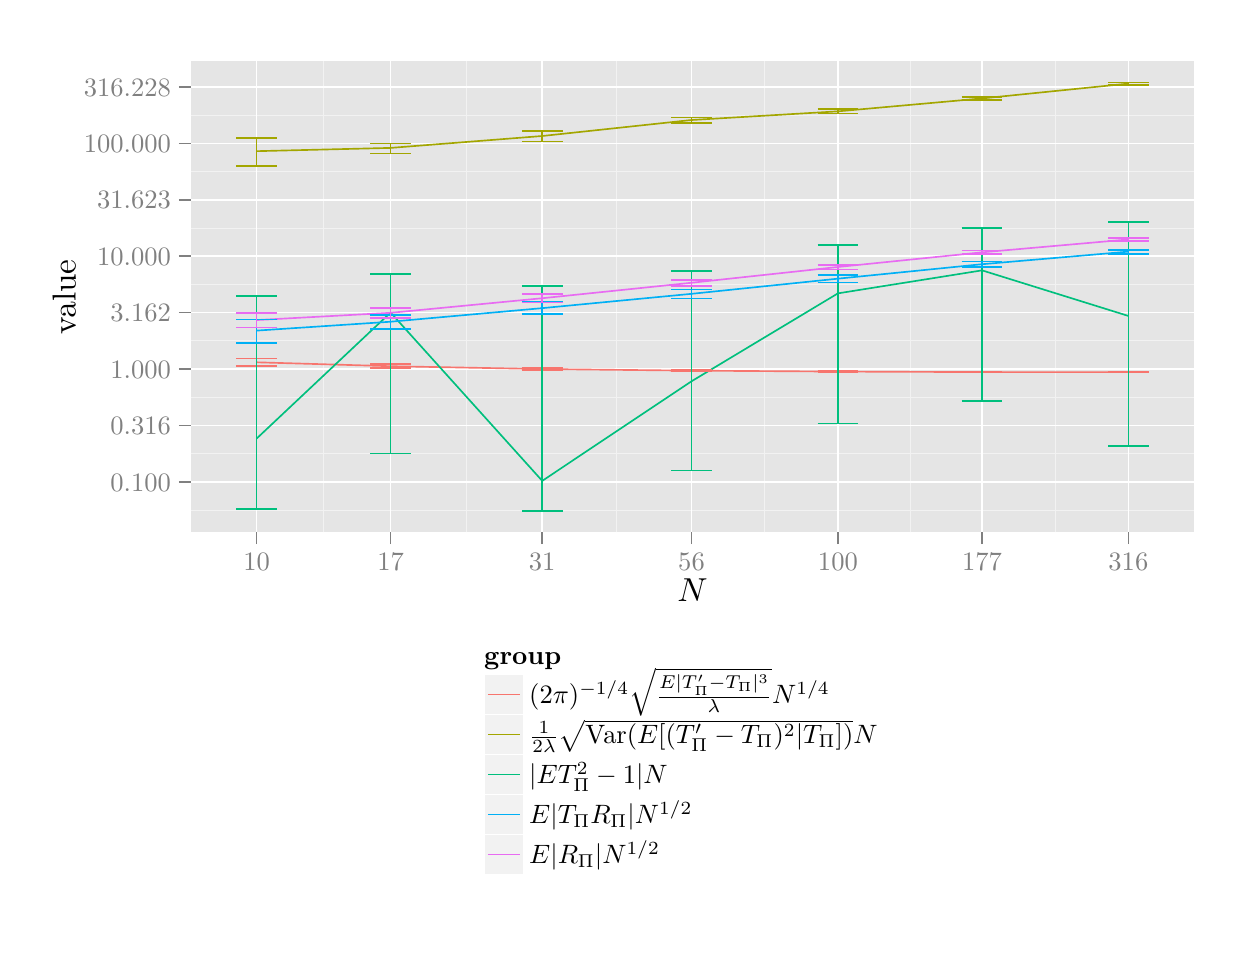
\begin{tikzpicture}[x=1pt,y=1pt]
\definecolor[named]{fillColor}{rgb}{1.00,1.00,1.00}
\path[use as bounding box,fill=fillColor,fill opacity=0.00] (0,0) rectangle (433.62,325.21);
\begin{scope}
\path[clip] (  0.00,  0.00) rectangle (433.62,325.21);
\definecolor[named]{drawColor}{rgb}{1.00,1.00,1.00}
\definecolor[named]{fillColor}{rgb}{1.00,1.00,1.00}

\path[draw=drawColor,line width= 0.6pt,line join=round,line cap=round,fill=fillColor] (  0.00,  0.00) rectangle (433.62,325.21);
\end{scope}
\begin{scope}
\path[clip] ( 58.88,142.81) rectangle (421.57,313.17);
\definecolor[named]{fillColor}{rgb}{0.90,0.90,0.90}

\path[fill=fillColor] ( 58.88,142.81) rectangle (421.57,313.17);
\definecolor[named]{drawColor}{rgb}{0.95,0.95,0.95}

\path[draw=drawColor,line width= 0.3pt,line join=round] ( 58.88,150.87) --
	(421.57,150.87);

\path[draw=drawColor,line width= 0.3pt,line join=round] ( 58.88,171.25) --
	(421.57,171.25);

\path[draw=drawColor,line width= 0.3pt,line join=round] ( 58.88,191.64) --
	(421.57,191.64);

\path[draw=drawColor,line width= 0.3pt,line join=round] ( 58.88,212.03) --
	(421.57,212.03);

\path[draw=drawColor,line width= 0.3pt,line join=round] ( 58.88,232.42) --
	(421.57,232.42);

\path[draw=drawColor,line width= 0.3pt,line join=round] ( 58.88,252.81) --
	(421.57,252.81);

\path[draw=drawColor,line width= 0.3pt,line join=round] ( 58.88,273.20) --
	(421.57,273.20);

\path[draw=drawColor,line width= 0.3pt,line join=round] ( 58.88,293.59) --
	(421.57,293.59);

\path[draw=drawColor,line width= 0.3pt,line join=round] (106.92,142.81) --
	(106.92,313.17);

\path[draw=drawColor,line width= 0.3pt,line join=round] (158.53,142.81) --
	(158.53,313.17);

\path[draw=drawColor,line width= 0.3pt,line join=round] (212.91,142.81) --
	(212.91,313.17);

\path[draw=drawColor,line width= 0.3pt,line join=round] (266.33,142.81) --
	(266.33,313.17);

\path[draw=drawColor,line width= 0.3pt,line join=round] (318.82,142.81) --
	(318.82,313.17);

\path[draw=drawColor,line width= 0.3pt,line join=round] (371.30,142.81) --
	(371.30,313.17);
\definecolor[named]{drawColor}{rgb}{1.00,1.00,1.00}

\path[draw=drawColor,line width= 0.6pt,line join=round] ( 58.88,161.06) --
	(421.57,161.06);

\path[draw=drawColor,line width= 0.6pt,line join=round] ( 58.88,181.44) --
	(421.57,181.44);

\path[draw=drawColor,line width= 0.6pt,line join=round] ( 58.88,201.84) --
	(421.57,201.84);

\path[draw=drawColor,line width= 0.6pt,line join=round] ( 58.88,222.23) --
	(421.57,222.23);

\path[draw=drawColor,line width= 0.6pt,line join=round] ( 58.88,242.62) --
	(421.57,242.62);

\path[draw=drawColor,line width= 0.6pt,line join=round] ( 58.88,263.01) --
	(421.57,263.01);

\path[draw=drawColor,line width= 0.6pt,line join=round] ( 58.88,283.39) --
	(421.57,283.39);

\path[draw=drawColor,line width= 0.6pt,line join=round] ( 58.88,303.78) --
	(421.57,303.78);

\path[draw=drawColor,line width= 0.6pt,line join=round] ( 82.72,142.81) --
	( 82.72,313.17);

\path[draw=drawColor,line width= 0.6pt,line join=round] (131.13,142.81) --
	(131.13,313.17);

\path[draw=drawColor,line width= 0.6pt,line join=round] (185.93,142.81) --
	(185.93,313.17);

\path[draw=drawColor,line width= 0.6pt,line join=round] (239.88,142.81) --
	(239.88,313.17);

\path[draw=drawColor,line width= 0.6pt,line join=round] (292.78,142.81) --
	(292.78,313.17);

\path[draw=drawColor,line width= 0.6pt,line join=round] (344.86,142.81) --
	(344.86,313.17);

\path[draw=drawColor,line width= 0.6pt,line join=round] (397.74,142.81) --
	(397.74,313.17);
\definecolor[named]{drawColor}{rgb}{0.97,0.46,0.43}

\path[draw=drawColor,line width= 0.6pt,line join=round] ( 82.72,204.29) --
	(131.13,202.88) --
	(185.93,201.85) --
	(239.88,201.27) --
	(292.78,200.94) --
	(344.86,200.75) --
	(397.74,200.74);
\definecolor[named]{drawColor}{rgb}{0.64,0.65,0.00}

\path[draw=drawColor,line width= 0.6pt,line join=round] ( 82.72,280.58) --
	(131.13,281.76) --
	(185.93,286.06) --
	(239.88,291.84) --
	(292.78,294.97) --
	(344.86,299.64) --
	(397.74,305.00);
\definecolor[named]{drawColor}{rgb}{0.00,0.75,0.49}

\path[draw=drawColor,line width= 0.6pt,line join=round] ( 82.72,176.72) --
	(131.13,222.28) --
	(185.93,161.45) --
	(239.88,197.43) --
	(292.78,229.20) --
	(344.86,237.51) --
	(397.74,221.04);
\definecolor[named]{drawColor}{rgb}{0.00,0.69,0.96}

\path[draw=drawColor,line width= 0.6pt,line join=round] ( 82.72,215.74) --
	(131.13,218.95) --
	(185.93,223.86) --
	(239.88,229.03) --
	(292.78,234.51) --
	(344.86,239.73) --
	(397.74,244.28);
\definecolor[named]{drawColor}{rgb}{0.91,0.42,0.95}

\path[draw=drawColor,line width= 0.6pt,line join=round] ( 82.72,219.55) --
	(131.13,222.17) --
	(185.93,227.44) --
	(239.88,233.03) --
	(292.78,238.73) --
	(344.86,244.03) --
	(397.74,248.68);
\definecolor[named]{drawColor}{rgb}{0.97,0.46,0.43}

\path[draw=drawColor,line width= 0.6pt,line join=round] ( 75.37,205.63) --
	( 90.07,205.63);

\path[draw=drawColor,line width= 0.6pt,line join=round] ( 82.72,205.63) --
	( 82.72,202.84);

\path[draw=drawColor,line width= 0.6pt,line join=round] ( 75.37,202.84) --
	( 90.07,202.84);

\path[draw=drawColor,line width= 0.6pt,line join=round] (123.78,203.60) --
	(138.48,203.60);

\path[draw=drawColor,line width= 0.6pt,line join=round] (131.13,203.60) --
	(131.13,202.14);

\path[draw=drawColor,line width= 0.6pt,line join=round] (123.78,202.14) --
	(138.48,202.14);

\path[draw=drawColor,line width= 0.6pt,line join=round] (178.58,202.27) --
	(193.28,202.27);

\path[draw=drawColor,line width= 0.6pt,line join=round] (185.93,202.27) --
	(185.93,201.45);

\path[draw=drawColor,line width= 0.6pt,line join=round] (178.58,201.45) --
	(193.28,201.45);

\path[draw=drawColor,line width= 0.6pt,line join=round] (232.53,201.49) --
	(247.23,201.49);

\path[draw=drawColor,line width= 0.6pt,line join=round] (239.88,201.49) --
	(239.88,201.06);

\path[draw=drawColor,line width= 0.6pt,line join=round] (232.53,201.06) --
	(247.23,201.06);

\path[draw=drawColor,line width= 0.6pt,line join=round] (285.42,201.05) --
	(300.13,201.05);

\path[draw=drawColor,line width= 0.6pt,line join=round] (292.78,201.05) --
	(292.78,200.83);

\path[draw=drawColor,line width= 0.6pt,line join=round] (285.42,200.83) --
	(300.13,200.83);

\path[draw=drawColor,line width= 0.6pt,line join=round] (337.51,200.81) --
	(352.22,200.81);

\path[draw=drawColor,line width= 0.6pt,line join=round] (344.86,200.81) --
	(344.86,200.68);

\path[draw=drawColor,line width= 0.6pt,line join=round] (337.51,200.68) --
	(352.22,200.68);

\path[draw=drawColor,line width= 0.6pt,line join=round] (390.39,200.77) --
	(405.09,200.77);

\path[draw=drawColor,line width= 0.6pt,line join=round] (397.74,200.77) --
	(397.74,200.70);

\path[draw=drawColor,line width= 0.6pt,line join=round] (390.39,200.70) --
	(405.09,200.70);
\definecolor[named]{drawColor}{rgb}{0.64,0.65,0.00}

\path[draw=drawColor,line width= 0.6pt,line join=round] ( 75.37,285.23) --
	( 90.07,285.23);

\path[draw=drawColor,line width= 0.6pt,line join=round] ( 82.72,285.23) --
	( 82.72,275.29);

\path[draw=drawColor,line width= 0.6pt,line join=round] ( 75.37,275.29) --
	( 90.07,275.29);

\path[draw=drawColor,line width= 0.6pt,line join=round] (123.78,283.32) --
	(138.48,283.32);

\path[draw=drawColor,line width= 0.6pt,line join=round] (131.13,283.32) --
	(131.13,279.79);

\path[draw=drawColor,line width= 0.6pt,line join=round] (123.78,279.79) --
	(138.48,279.79);

\path[draw=drawColor,line width= 0.6pt,line join=round] (178.58,287.96) --
	(193.28,287.96);

\path[draw=drawColor,line width= 0.6pt,line join=round] (185.93,287.96) --
	(185.93,284.11);

\path[draw=drawColor,line width= 0.6pt,line join=round] (178.58,284.11) --
	(193.28,284.11);

\path[draw=drawColor,line width= 0.6pt,line join=round] (232.53,292.76) --
	(247.23,292.76);

\path[draw=drawColor,line width= 0.6pt,line join=round] (239.88,292.76) --
	(239.88,290.83);

\path[draw=drawColor,line width= 0.6pt,line join=round] (232.53,290.83) --
	(247.23,290.83);

\path[draw=drawColor,line width= 0.6pt,line join=round] (285.42,295.73) --
	(300.13,295.73);

\path[draw=drawColor,line width= 0.6pt,line join=round] (292.78,295.73) --
	(292.78,294.20);

\path[draw=drawColor,line width= 0.6pt,line join=round] (285.42,294.20) --
	(300.13,294.20);

\path[draw=drawColor,line width= 0.6pt,line join=round] (337.51,300.16) --
	(352.22,300.16);

\path[draw=drawColor,line width= 0.6pt,line join=round] (344.86,300.16) --
	(344.86,298.98);

\path[draw=drawColor,line width= 0.6pt,line join=round] (337.51,298.98) --
	(352.22,298.98);

\path[draw=drawColor,line width= 0.6pt,line join=round] (390.39,305.43) --
	(405.09,305.43);

\path[draw=drawColor,line width= 0.6pt,line join=round] (397.74,305.43) --
	(397.74,304.57);

\path[draw=drawColor,line width= 0.6pt,line join=round] (390.39,304.57) --
	(405.09,304.57);
\definecolor[named]{drawColor}{rgb}{0.00,0.75,0.49}

\path[draw=drawColor,line width= 0.6pt,line join=round] ( 75.37,228.34) --
	( 90.07,228.34);

\path[draw=drawColor,line width= 0.6pt,line join=round] ( 82.72,228.34) --
	( 82.72,151.28);

\path[draw=drawColor,line width= 0.6pt,line join=round] ( 75.37,151.28) --
	( 90.07,151.28);

\path[draw=drawColor,line width= 0.6pt,line join=round] (123.78,236.31) --
	(138.48,236.31);

\path[draw=drawColor,line width= 0.6pt,line join=round] (131.13,236.31) --
	(131.13,171.31);

\path[draw=drawColor,line width= 0.6pt,line join=round] (123.78,171.31) --
	(138.48,171.31);

\path[draw=drawColor,line width= 0.6pt,line join=round] (178.58,231.87) --
	(193.28,231.87);

\path[draw=drawColor,line width= 0.6pt,line join=round] (185.93,231.87) --
	(185.93,150.56);

\path[draw=drawColor,line width= 0.6pt,line join=round] (178.58,150.56) --
	(193.28,150.56);

\path[draw=drawColor,line width= 0.6pt,line join=round] (232.53,237.27) --
	(247.23,237.27);

\path[draw=drawColor,line width= 0.6pt,line join=round] (239.88,237.27) --
	(239.88,165.14);

\path[draw=drawColor,line width= 0.6pt,line join=round] (232.53,165.14) --
	(247.23,165.14);

\path[draw=drawColor,line width= 0.6pt,line join=round] (285.42,246.62) --
	(300.13,246.62);

\path[draw=drawColor,line width= 0.6pt,line join=round] (292.78,246.62) --
	(292.78,182.18);

\path[draw=drawColor,line width= 0.6pt,line join=round] (285.42,182.18) --
	(300.13,182.18);

\path[draw=drawColor,line width= 0.6pt,line join=round] (337.51,252.84) --
	(352.22,252.84);

\path[draw=drawColor,line width= 0.6pt,line join=round] (344.86,252.84) --
	(344.86,190.19);

\path[draw=drawColor,line width= 0.6pt,line join=round] (337.51,190.19) --
	(352.22,190.19);

\path[draw=drawColor,line width= 0.6pt,line join=round] (390.39,255.07) --
	(405.09,255.07);

\path[draw=drawColor,line width= 0.6pt,line join=round] (397.74,255.07) --
	(397.74,174.12);

\path[draw=drawColor,line width= 0.6pt,line join=round] (390.39,174.12) --
	(405.09,174.12);
\definecolor[named]{drawColor}{rgb}{0.00,0.69,0.96}

\path[draw=drawColor,line width= 0.6pt,line join=round] ( 75.37,219.70) --
	( 90.07,219.70);

\path[draw=drawColor,line width= 0.6pt,line join=round] ( 82.72,219.70) --
	( 82.72,211.37);

\path[draw=drawColor,line width= 0.6pt,line join=round] ( 75.37,211.37) --
	( 90.07,211.37);

\path[draw=drawColor,line width= 0.6pt,line join=round] (123.78,221.50) --
	(138.48,221.50);

\path[draw=drawColor,line width= 0.6pt,line join=round] (131.13,221.50) --
	(131.13,216.27);

\path[draw=drawColor,line width= 0.6pt,line join=round] (123.78,216.27) --
	(138.48,216.27);

\path[draw=drawColor,line width= 0.6pt,line join=round] (178.58,226.01) --
	(193.28,226.01);

\path[draw=drawColor,line width= 0.6pt,line join=round] (185.93,226.01) --
	(185.93,221.63);

\path[draw=drawColor,line width= 0.6pt,line join=round] (178.58,221.63) --
	(193.28,221.63);

\path[draw=drawColor,line width= 0.6pt,line join=round] (232.53,230.64) --
	(247.23,230.64);

\path[draw=drawColor,line width= 0.6pt,line join=round] (239.88,230.64) --
	(239.88,227.29);

\path[draw=drawColor,line width= 0.6pt,line join=round] (232.53,227.29) --
	(247.23,227.29);

\path[draw=drawColor,line width= 0.6pt,line join=round] (285.42,235.90) --
	(300.13,235.90);

\path[draw=drawColor,line width= 0.6pt,line join=round] (292.78,235.90) --
	(292.78,233.12);

\path[draw=drawColor,line width= 0.6pt,line join=round] (285.42,233.12) --
	(300.13,233.12);

\path[draw=drawColor,line width= 0.6pt,line join=round] (337.51,240.73) --
	(352.22,240.73);

\path[draw=drawColor,line width= 0.6pt,line join=round] (344.86,240.73) --
	(344.86,238.72);

\path[draw=drawColor,line width= 0.6pt,line join=round] (337.51,238.72) --
	(352.22,238.72);

\path[draw=drawColor,line width= 0.6pt,line join=round] (390.39,244.97) --
	(405.09,244.97);

\path[draw=drawColor,line width= 0.6pt,line join=round] (397.74,244.97) --
	(397.74,243.46);

\path[draw=drawColor,line width= 0.6pt,line join=round] (390.39,243.46) --
	(405.09,243.46);
\definecolor[named]{drawColor}{rgb}{0.91,0.42,0.95}

\path[draw=drawColor,line width= 0.6pt,line join=round] ( 75.37,222.00) --
	( 90.07,222.00);

\path[draw=drawColor,line width= 0.6pt,line join=round] ( 82.72,222.00) --
	( 82.72,216.86);

\path[draw=drawColor,line width= 0.6pt,line join=round] ( 75.37,216.86) --
	( 90.07,216.86);

\path[draw=drawColor,line width= 0.6pt,line join=round] (123.78,223.91) --
	(138.48,223.91);

\path[draw=drawColor,line width= 0.6pt,line join=round] (131.13,223.91) --
	(131.13,220.37);

\path[draw=drawColor,line width= 0.6pt,line join=round] (123.78,220.37) --
	(138.48,220.37);

\path[draw=drawColor,line width= 0.6pt,line join=round] (178.58,228.92) --
	(193.28,228.92);

\path[draw=drawColor,line width= 0.6pt,line join=round] (185.93,228.92) --
	(185.93,225.87);

\path[draw=drawColor,line width= 0.6pt,line join=round] (178.58,225.87) --
	(193.28,225.87);

\path[draw=drawColor,line width= 0.6pt,line join=round] (232.53,234.09) --
	(247.23,234.09);

\path[draw=drawColor,line width= 0.6pt,line join=round] (239.88,234.09) --
	(239.88,231.95);

\path[draw=drawColor,line width= 0.6pt,line join=round] (232.53,231.95) --
	(247.23,231.95);

\path[draw=drawColor,line width= 0.6pt,line join=round] (285.42,239.53) --
	(300.13,239.53);

\path[draw=drawColor,line width= 0.6pt,line join=round] (292.78,239.53) --
	(292.78,237.86);

\path[draw=drawColor,line width= 0.6pt,line join=round] (285.42,237.86) --
	(300.13,237.86);

\path[draw=drawColor,line width= 0.6pt,line join=round] (337.51,244.68) --
	(352.22,244.68);

\path[draw=drawColor,line width= 0.6pt,line join=round] (344.86,244.68) --
	(344.86,243.41);

\path[draw=drawColor,line width= 0.6pt,line join=round] (337.51,243.41) --
	(352.22,243.41);

\path[draw=drawColor,line width= 0.6pt,line join=round] (390.39,249.15) --
	(405.09,249.15);

\path[draw=drawColor,line width= 0.6pt,line join=round] (397.74,249.15) --
	(397.74,248.19);

\path[draw=drawColor,line width= 0.6pt,line join=round] (390.39,248.19) --
	(405.09,248.19);
\end{scope}
\begin{scope}
\path[clip] (  0.00,  0.00) rectangle (433.62,325.21);
\definecolor[named]{drawColor}{rgb}{0.50,0.50,0.50}

\node[text=drawColor,anchor=base east,inner sep=0pt, outer sep=0pt, scale=  0.96] at ( 51.77,157.75) {0.100};

\node[text=drawColor,anchor=base east,inner sep=0pt, outer sep=0pt, scale=  0.96] at ( 51.77,178.13) {0.316};

\node[text=drawColor,anchor=base east,inner sep=0pt, outer sep=0pt, scale=  0.96] at ( 51.77,198.53) {1.000};

\node[text=drawColor,anchor=base east,inner sep=0pt, outer sep=0pt, scale=  0.96] at ( 51.77,218.92) {3.162};

\node[text=drawColor,anchor=base east,inner sep=0pt, outer sep=0pt, scale=  0.96] at ( 51.77,239.31) {10.000};

\node[text=drawColor,anchor=base east,inner sep=0pt, outer sep=0pt, scale=  0.96] at ( 51.77,259.70) {31.623};

\node[text=drawColor,anchor=base east,inner sep=0pt, outer sep=0pt, scale=  0.96] at ( 51.77,280.09) {100.000};

\node[text=drawColor,anchor=base east,inner sep=0pt, outer sep=0pt, scale=  0.96] at ( 51.77,300.48) {316.228};
\end{scope}
\begin{scope}
\path[clip] (  0.00,  0.00) rectangle (433.62,325.21);
\definecolor[named]{drawColor}{rgb}{0.50,0.50,0.50}

\path[draw=drawColor,line width= 0.6pt,line join=round] ( 54.61,161.06) --
	( 58.88,161.06);

\path[draw=drawColor,line width= 0.6pt,line join=round] ( 54.61,181.44) --
	( 58.88,181.44);

\path[draw=drawColor,line width= 0.6pt,line join=round] ( 54.61,201.84) --
	( 58.88,201.84);

\path[draw=drawColor,line width= 0.6pt,line join=round] ( 54.61,222.23) --
	( 58.88,222.23);

\path[draw=drawColor,line width= 0.6pt,line join=round] ( 54.61,242.62) --
	( 58.88,242.62);

\path[draw=drawColor,line width= 0.6pt,line join=round] ( 54.61,263.01) --
	( 58.88,263.01);

\path[draw=drawColor,line width= 0.6pt,line join=round] ( 54.61,283.39) --
	( 58.88,283.39);

\path[draw=drawColor,line width= 0.6pt,line join=round] ( 54.61,303.78) --
	( 58.88,303.78);
\end{scope}
\begin{scope}
\path[clip] (  0.00,  0.00) rectangle (433.62,325.21);
\definecolor[named]{drawColor}{rgb}{0.50,0.50,0.50}

\path[draw=drawColor,line width= 0.6pt,line join=round] ( 82.72,138.55) --
	( 82.72,142.81);

\path[draw=drawColor,line width= 0.6pt,line join=round] (131.13,138.55) --
	(131.13,142.81);

\path[draw=drawColor,line width= 0.6pt,line join=round] (185.93,138.55) --
	(185.93,142.81);

\path[draw=drawColor,line width= 0.6pt,line join=round] (239.88,138.55) --
	(239.88,142.81);

\path[draw=drawColor,line width= 0.6pt,line join=round] (292.78,138.55) --
	(292.78,142.81);

\path[draw=drawColor,line width= 0.6pt,line join=round] (344.86,138.55) --
	(344.86,142.81);

\path[draw=drawColor,line width= 0.6pt,line join=round] (397.74,138.55) --
	(397.74,142.81);
\end{scope}
\begin{scope}
\path[clip] (  0.00,  0.00) rectangle (433.62,325.21);
\definecolor[named]{drawColor}{rgb}{0.50,0.50,0.50}

\node[text=drawColor,anchor=base,inner sep=0pt, outer sep=0pt, scale=  0.96] at ( 82.72,129.09) {10};

\node[text=drawColor,anchor=base,inner sep=0pt, outer sep=0pt, scale=  0.96] at (131.13,129.09) {17};

\node[text=drawColor,anchor=base,inner sep=0pt, outer sep=0pt, scale=  0.96] at (185.93,129.09) {31};

\node[text=drawColor,anchor=base,inner sep=0pt, outer sep=0pt, scale=  0.96] at (239.88,129.09) {56};

\node[text=drawColor,anchor=base,inner sep=0pt, outer sep=0pt, scale=  0.96] at (292.78,129.09) {100};

\node[text=drawColor,anchor=base,inner sep=0pt, outer sep=0pt, scale=  0.96] at (344.86,129.09) {177};

\node[text=drawColor,anchor=base,inner sep=0pt, outer sep=0pt, scale=  0.96] at (397.74,129.09) {316};
\end{scope}
\begin{scope}
\path[clip] (  0.00,  0.00) rectangle (433.62,325.21);
\definecolor[named]{drawColor}{rgb}{0.00,0.00,0.00}

\node[text=drawColor,anchor=base,inner sep=0pt, outer sep=0pt, scale=  1.20] at (240.23,117.81) {$N$};
\end{scope}
\begin{scope}
\path[clip] (  0.00,  0.00) rectangle (433.62,325.21);
\definecolor[named]{drawColor}{rgb}{0.00,0.00,0.00}

\node[text=drawColor,rotate= 90.00,anchor=base,inner sep=0pt, outer sep=0pt, scale=  1.20] at ( 17.30,227.99) {value};
\end{scope}
\begin{scope}
\path[clip] (  0.00,  0.00) rectangle (433.62,325.21);
\definecolor[named]{fillColor}{rgb}{1.00,1.00,1.00}

\path[fill=fillColor] (160.71, 14.89) rectangle (319.75,105.93);
\end{scope}
\begin{scope}
\path[clip] (  0.00,  0.00) rectangle (433.62,325.21);
\definecolor[named]{drawColor}{rgb}{0.00,0.00,0.00}

\node[text=drawColor,anchor=base west,inner sep=0pt, outer sep=0pt, scale=  0.96] at (164.98, 95.04) {\bfseries group};
\end{scope}
\begin{scope}
\path[clip] (  0.00,  0.00) rectangle (433.62,325.21);
\definecolor[named]{drawColor}{rgb}{1.00,1.00,1.00}
\definecolor[named]{fillColor}{rgb}{0.95,0.95,0.95}

\path[draw=drawColor,line width= 0.6pt,line join=round,line cap=round,fill=fillColor] (164.98, 76.97) rectangle (179.43, 91.43);
\end{scope}
\begin{scope}
\path[clip] (  0.00,  0.00) rectangle (433.62,325.21);
\definecolor[named]{drawColor}{rgb}{0.97,0.46,0.43}

\path[draw=drawColor,line width= 0.6pt,line join=round] (166.42, 84.20) -- (177.98, 84.20);
\end{scope}
\begin{scope}
\path[clip] (  0.00,  0.00) rectangle (433.62,325.21);
\definecolor[named]{drawColor}{rgb}{0.97,0.46,0.43}

\path[draw=drawColor,line width= 0.6pt,line join=round] (166.42, 84.20) -- (177.98, 84.20);
\end{scope}
\begin{scope}
\path[clip] (  0.00,  0.00) rectangle (433.62,325.21);
\definecolor[named]{drawColor}{rgb}{1.00,1.00,1.00}
\definecolor[named]{fillColor}{rgb}{0.95,0.95,0.95}

\path[draw=drawColor,line width= 0.6pt,line join=round,line cap=round,fill=fillColor] (164.98, 62.52) rectangle (179.43, 76.97);
\end{scope}
\begin{scope}
\path[clip] (  0.00,  0.00) rectangle (433.62,325.21);
\definecolor[named]{drawColor}{rgb}{0.64,0.65,0.00}

\path[draw=drawColor,line width= 0.6pt,line join=round] (166.42, 69.75) -- (177.98, 69.75);
\end{scope}
\begin{scope}
\path[clip] (  0.00,  0.00) rectangle (433.62,325.21);
\definecolor[named]{drawColor}{rgb}{0.64,0.65,0.00}

\path[draw=drawColor,line width= 0.6pt,line join=round] (166.42, 69.75) -- (177.98, 69.75);
\end{scope}
\begin{scope}
\path[clip] (  0.00,  0.00) rectangle (433.62,325.21);
\definecolor[named]{drawColor}{rgb}{1.00,1.00,1.00}
\definecolor[named]{fillColor}{rgb}{0.95,0.95,0.95}

\path[draw=drawColor,line width= 0.6pt,line join=round,line cap=round,fill=fillColor] (164.98, 48.07) rectangle (179.43, 62.52);
\end{scope}
\begin{scope}
\path[clip] (  0.00,  0.00) rectangle (433.62,325.21);
\definecolor[named]{drawColor}{rgb}{0.00,0.75,0.49}

\path[draw=drawColor,line width= 0.6pt,line join=round] (166.42, 55.29) -- (177.98, 55.29);
\end{scope}
\begin{scope}
\path[clip] (  0.00,  0.00) rectangle (433.62,325.21);
\definecolor[named]{drawColor}{rgb}{0.00,0.75,0.49}

\path[draw=drawColor,line width= 0.6pt,line join=round] (166.42, 55.29) -- (177.98, 55.29);
\end{scope}
\begin{scope}
\path[clip] (  0.00,  0.00) rectangle (433.62,325.21);
\definecolor[named]{drawColor}{rgb}{1.00,1.00,1.00}
\definecolor[named]{fillColor}{rgb}{0.95,0.95,0.95}

\path[draw=drawColor,line width= 0.6pt,line join=round,line cap=round,fill=fillColor] (164.98, 33.61) rectangle (179.43, 48.07);
\end{scope}
\begin{scope}
\path[clip] (  0.00,  0.00) rectangle (433.62,325.21);
\definecolor[named]{drawColor}{rgb}{0.00,0.69,0.96}

\path[draw=drawColor,line width= 0.6pt,line join=round] (166.42, 40.84) -- (177.98, 40.84);
\end{scope}
\begin{scope}
\path[clip] (  0.00,  0.00) rectangle (433.62,325.21);
\definecolor[named]{drawColor}{rgb}{0.00,0.69,0.96}

\path[draw=drawColor,line width= 0.6pt,line join=round] (166.42, 40.84) -- (177.98, 40.84);
\end{scope}
\begin{scope}
\path[clip] (  0.00,  0.00) rectangle (433.62,325.21);
\definecolor[named]{drawColor}{rgb}{1.00,1.00,1.00}
\definecolor[named]{fillColor}{rgb}{0.95,0.95,0.95}

\path[draw=drawColor,line width= 0.6pt,line join=round,line cap=round,fill=fillColor] (164.98, 19.16) rectangle (179.43, 33.61);
\end{scope}
\begin{scope}
\path[clip] (  0.00,  0.00) rectangle (433.62,325.21);
\definecolor[named]{drawColor}{rgb}{0.91,0.42,0.95}

\path[draw=drawColor,line width= 0.6pt,line join=round] (166.42, 26.39) -- (177.98, 26.39);
\end{scope}
\begin{scope}
\path[clip] (  0.00,  0.00) rectangle (433.62,325.21);
\definecolor[named]{drawColor}{rgb}{0.91,0.42,0.95}

\path[draw=drawColor,line width= 0.6pt,line join=round] (166.42, 26.39) -- (177.98, 26.39);
\end{scope}
\begin{scope}
\path[clip] (  0.00,  0.00) rectangle (433.62,325.21);
\definecolor[named]{drawColor}{rgb}{0.00,0.00,0.00}

\node[text=drawColor,anchor=base west,inner sep=0pt, outer sep=0pt, scale=  0.96] at (181.24, 80.90) {$(2\pi)^{-1/4}\sqrt{\frac{\mathbb{E}|T'_{\Pi}-T_{\Pi}|^3}{\lambda}}N^{1/4}\quad $};
\end{scope}
\begin{scope}
\path[clip] (  0.00,  0.00) rectangle (433.62,325.21);
\definecolor[named]{drawColor}{rgb}{0.00,0.00,0.00}

\node[text=drawColor,anchor=base west,inner sep=0pt, outer sep=0pt, scale=  0.96] at (181.24, 66.44) {$\frac{1}{2\lambda}\sqrt{\mathrm{Var}(\mathbb{E}[(T'_{\Pi}-T_{\Pi})^2|T_{\Pi}])}N\quad $};
\end{scope}
\begin{scope}
\path[clip] (  0.00,  0.00) rectangle (433.62,325.21);
\definecolor[named]{drawColor}{rgb}{0.00,0.00,0.00}

\node[text=drawColor,anchor=base west,inner sep=0pt, outer sep=0pt, scale=  0.96] at (181.24, 51.99) {$|\mathbb{E}T_{\Pi}^2-1|N\quad $};
\end{scope}
\begin{scope}
\path[clip] (  0.00,  0.00) rectangle (433.62,325.21);
\definecolor[named]{drawColor}{rgb}{0.00,0.00,0.00}

\node[text=drawColor,anchor=base west,inner sep=0pt, outer sep=0pt, scale=  0.96] at (181.24, 37.53) {$\mathbb{E}|T_{\Pi}R_{\Pi}|N^{1/2}\quad $};
\end{scope}
\begin{scope}
\path[clip] (  0.00,  0.00) rectangle (433.62,325.21);
\definecolor[named]{drawColor}{rgb}{0.00,0.00,0.00}

\node[text=drawColor,anchor=base west,inner sep=0pt, outer sep=0pt, scale=  0.96] at (181.24, 23.08) {$\mathbb{E}|R_{\Pi}|N^{1/2}\quad $};
\end{scope}
\end{tikzpicture}

  \caption{Log-log plot of values for each term in the bound,
    simulating the conditional by Monte Carlo.}
\end{figure}
The MC error is too large, and we see some scaled bounds actually increase.
\clearpage

\subsection{Exact Conditional Expectation Calculations}
Motivated by the Monte Carlo error in estimating the conditional expectations
$\E[f(T'_{\Pi}, T_{\Pi}) | T_{\Pi}]$, we describe an efficient procedure to
calculate all values $T'$ corresponding to a given $T$ exactly in Section~\ref{S:efficient-updates}.
We still use Monte Carlo simulations to calculate a subset of all the permutations $\Pi$, otherwise
the computational cost would be prohibitive for large sample sizes.
\begin{figure}[!ht]
  \centering
  % Created by tikzDevice version 0.6.2-92-0ad2792 on 2013-05-05 16:12:42
% !TEX encoding = UTF-8 Unicode
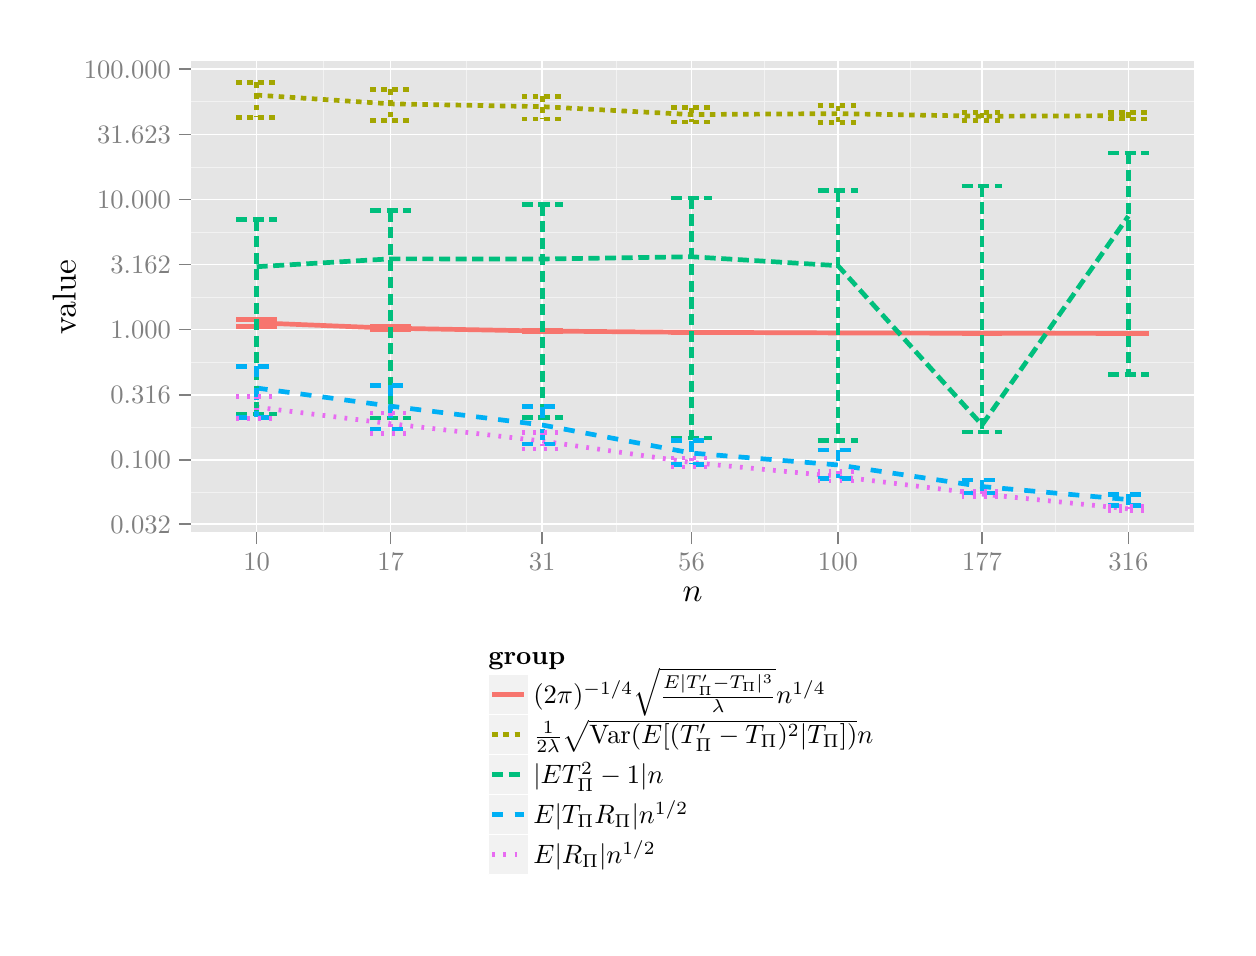
\begin{tikzpicture}[x=1pt,y=1pt]
\definecolor[named]{fillColor}{rgb}{1.00,1.00,1.00}
\path[use as bounding box,fill=fillColor,fill opacity=0.00] (0,0) rectangle (433.62,325.21);
\begin{scope}
\path[clip] (  0.00,  0.00) rectangle (433.62,325.21);
\definecolor[named]{drawColor}{rgb}{1.00,1.00,1.00}
\definecolor[named]{fillColor}{rgb}{1.00,1.00,1.00}

\path[draw=drawColor,line width= 0.6pt,line join=round,line cap=round,fill=fillColor] (  0.00,  0.00) rectangle (433.62,325.21);
\end{scope}
\begin{scope}
\path[clip] ( 58.88,142.81) rectangle (421.57,313.17);
\definecolor[named]{fillColor}{rgb}{0.90,0.90,0.90}

\path[fill=fillColor] ( 58.88,142.81) rectangle (421.57,313.17);
\definecolor[named]{drawColor}{rgb}{0.95,0.95,0.95}

\path[draw=drawColor,line width= 0.3pt,line join=round] ( 58.88,157.41) --
	(421.57,157.41);

\path[draw=drawColor,line width= 0.3pt,line join=round] ( 58.88,180.80) --
	(421.57,180.80);

\path[draw=drawColor,line width= 0.3pt,line join=round] ( 58.88,204.32) --
	(421.57,204.32);

\path[draw=drawColor,line width= 0.3pt,line join=round] ( 58.88,227.85) --
	(421.57,227.85);

\path[draw=drawColor,line width= 0.3pt,line join=round] ( 58.88,251.37) --
	(421.57,251.37);

\path[draw=drawColor,line width= 0.3pt,line join=round] ( 58.88,274.89) --
	(421.57,274.89);

\path[draw=drawColor,line width= 0.3pt,line join=round] ( 58.88,298.41) --
	(421.57,298.41);

\path[draw=drawColor,line width= 0.3pt,line join=round] (106.92,142.81) --
	(106.92,313.17);

\path[draw=drawColor,line width= 0.3pt,line join=round] (158.53,142.81) --
	(158.53,313.17);

\path[draw=drawColor,line width= 0.3pt,line join=round] (212.91,142.81) --
	(212.91,313.17);

\path[draw=drawColor,line width= 0.3pt,line join=round] (266.33,142.81) --
	(266.33,313.17);

\path[draw=drawColor,line width= 0.3pt,line join=round] (318.82,142.81) --
	(318.82,313.17);

\path[draw=drawColor,line width= 0.3pt,line join=round] (371.30,142.81) --
	(371.30,313.17);
\definecolor[named]{drawColor}{rgb}{1.00,1.00,1.00}

\path[draw=drawColor,line width= 0.6pt,line join=round] ( 58.88,145.77) --
	(421.57,145.77);

\path[draw=drawColor,line width= 0.6pt,line join=round] ( 58.88,169.05) --
	(421.57,169.05);

\path[draw=drawColor,line width= 0.6pt,line join=round] ( 58.88,192.56) --
	(421.57,192.56);

\path[draw=drawColor,line width= 0.6pt,line join=round] ( 58.88,216.09) --
	(421.57,216.09);

\path[draw=drawColor,line width= 0.6pt,line join=round] ( 58.88,239.61) --
	(421.57,239.61);

\path[draw=drawColor,line width= 0.6pt,line join=round] ( 58.88,263.13) --
	(421.57,263.13);

\path[draw=drawColor,line width= 0.6pt,line join=round] ( 58.88,286.65) --
	(421.57,286.65);

\path[draw=drawColor,line width= 0.6pt,line join=round] ( 58.88,310.17) --
	(421.57,310.17);

\path[draw=drawColor,line width= 0.6pt,line join=round] ( 82.72,142.81) --
	( 82.72,313.17);

\path[draw=drawColor,line width= 0.6pt,line join=round] (131.13,142.81) --
	(131.13,313.17);

\path[draw=drawColor,line width= 0.6pt,line join=round] (185.93,142.81) --
	(185.93,313.17);

\path[draw=drawColor,line width= 0.6pt,line join=round] (239.88,142.81) --
	(239.88,313.17);

\path[draw=drawColor,line width= 0.6pt,line join=round] (292.78,142.81) --
	(292.78,313.17);

\path[draw=drawColor,line width= 0.6pt,line join=round] (344.86,142.81) --
	(344.86,313.17);

\path[draw=drawColor,line width= 0.6pt,line join=round] (397.74,142.81) --
	(397.74,313.17);
\definecolor[named]{drawColor}{rgb}{0.97,0.46,0.43}

\path[draw=drawColor,line width= 1.7pt,line join=round] ( 82.72,218.56) --
	(131.13,216.61) --
	(185.93,215.59) --
	(239.88,215.11) --
	(292.78,214.90) --
	(344.86,214.78) --
	(397.74,214.72);
\definecolor[named]{drawColor}{rgb}{0.64,0.65,0.00}

\path[draw=drawColor,line width= 1.7pt,dash pattern=on 2pt off 2pt ,line join=round] ( 82.72,300.84) --
	(131.13,297.68) --
	(185.93,296.66) --
	(239.88,293.81) --
	(292.78,294.15) --
	(344.86,293.20) --
	(397.74,293.39);
\definecolor[named]{drawColor}{rgb}{0.00,0.75,0.49}

\path[draw=drawColor,line width= 1.7pt,dash pattern=on 4pt off 2pt ,line join=round] ( 82.72,238.83) --
	(131.13,241.67) --
	(185.93,241.62) --
	(239.88,242.43) --
	(292.78,239.21) --
	(344.86,181.65) --
	(397.74,257.10);
\definecolor[named]{drawColor}{rgb}{0.00,0.69,0.96}

\path[draw=drawColor,line width= 1.7pt,dash pattern=on 4pt off 4pt ,line join=round] ( 82.72,195.00) --
	(131.13,188.45) --
	(185.93,181.64) --
	(239.88,171.49) --
	(292.78,167.20) --
	(344.86,159.39) --
	(397.74,154.68);
\definecolor[named]{drawColor}{rgb}{0.91,0.42,0.95}

\path[draw=drawColor,line width= 1.7pt,dash pattern=on 1pt off 3pt ,line join=round] ( 82.72,188.07) --
	(131.13,182.11) --
	(185.93,175.83) --
	(239.88,168.07) --
	(292.78,163.05) --
	(344.86,156.66) --
	(397.74,151.34);
\definecolor[named]{drawColor}{rgb}{0.97,0.46,0.43}

\path[draw=drawColor,line width= 1.7pt,line join=round] ( 75.37,219.86) --
	( 90.07,219.86);

\path[draw=drawColor,line width= 1.7pt,line join=round] ( 82.72,219.86) --
	( 82.72,217.25);

\path[draw=drawColor,line width= 1.7pt,line join=round] ( 75.37,217.25) --
	( 90.07,217.25);

\path[draw=drawColor,line width= 1.7pt,line join=round] (123.78,217.20) --
	(138.48,217.20);

\path[draw=drawColor,line width= 1.7pt,line join=round] (131.13,217.20) --
	(131.13,216.13);

\path[draw=drawColor,line width= 1.7pt,line join=round] (123.78,216.13) --
	(138.48,216.13);

\path[draw=drawColor,line width= 1.7pt,line join=round] (178.58,215.80) --
	(193.28,215.80);

\path[draw=drawColor,line width= 1.7pt,line join=round] (185.93,215.80) --
	(185.93,215.40);

\path[draw=drawColor,line width= 1.7pt,line join=round] (178.58,215.40) --
	(193.28,215.40);

\path[draw=drawColor,line width= 1.7pt,line join=round] (232.53,215.18) --
	(247.23,215.18);

\path[draw=drawColor,line width= 1.7pt,line join=round] (239.88,215.18) --
	(239.88,215.05);

\path[draw=drawColor,line width= 1.7pt,line join=round] (232.53,215.05) --
	(247.23,215.05);

\path[draw=drawColor,line width= 1.7pt,line join=round] (285.42,214.93) --
	(300.13,214.93);

\path[draw=drawColor,line width= 1.7pt,line join=round] (292.78,214.93) --
	(292.78,214.87);

\path[draw=drawColor,line width= 1.7pt,line join=round] (285.42,214.87) --
	(300.13,214.87);

\path[draw=drawColor,line width= 1.7pt,line join=round] (337.51,214.80) --
	(352.22,214.80);

\path[draw=drawColor,line width= 1.7pt,line join=round] (344.86,214.80) --
	(344.86,214.77);

\path[draw=drawColor,line width= 1.7pt,line join=round] (337.51,214.77) --
	(352.22,214.77);

\path[draw=drawColor,line width= 1.7pt,line join=round] (390.39,214.73) --
	(405.09,214.73);

\path[draw=drawColor,line width= 1.7pt,line join=round] (397.74,214.73) --
	(397.74,214.72);

\path[draw=drawColor,line width= 1.7pt,line join=round] (390.39,214.72) --
	(405.09,214.72);
\definecolor[named]{drawColor}{rgb}{0.64,0.65,0.00}

\path[draw=drawColor,line width= 1.7pt,dash pattern=on 2pt off 2pt ,line join=round] ( 75.37,305.43) --
	( 90.07,305.43);

\path[draw=drawColor,line width= 1.7pt,dash pattern=on 2pt off 2pt ,line join=round] ( 82.72,305.43) --
	( 82.72,292.80);

\path[draw=drawColor,line width= 1.7pt,dash pattern=on 2pt off 2pt ,line join=round] ( 75.37,292.80) --
	( 90.07,292.80);

\path[draw=drawColor,line width= 1.7pt,dash pattern=on 2pt off 2pt ,line join=round] (123.78,302.89) --
	(138.48,302.89);

\path[draw=drawColor,line width= 1.7pt,dash pattern=on 2pt off 2pt ,line join=round] (131.13,302.89) --
	(131.13,291.54);

\path[draw=drawColor,line width= 1.7pt,dash pattern=on 2pt off 2pt ,line join=round] (123.78,291.54) --
	(138.48,291.54);

\path[draw=drawColor,line width= 1.7pt,dash pattern=on 2pt off 2pt ,line join=round] (178.58,300.41) --
	(193.28,300.41);

\path[draw=drawColor,line width= 1.7pt,dash pattern=on 2pt off 2pt ,line join=round] (185.93,300.41) --
	(185.93,292.16);

\path[draw=drawColor,line width= 1.7pt,dash pattern=on 2pt off 2pt ,line join=round] (178.58,292.16) --
	(193.28,292.16);

\path[draw=drawColor,line width= 1.7pt,dash pattern=on 2pt off 2pt ,line join=round] (232.53,296.25) --
	(247.23,296.25);

\path[draw=drawColor,line width= 1.7pt,dash pattern=on 2pt off 2pt ,line join=round] (239.88,296.25) --
	(239.88,291.11);

\path[draw=drawColor,line width= 1.7pt,dash pattern=on 2pt off 2pt ,line join=round] (232.53,291.11) --
	(247.23,291.11);

\path[draw=drawColor,line width= 1.7pt,dash pattern=on 2pt off 2pt ,line join=round] (285.42,297.07) --
	(300.13,297.07);

\path[draw=drawColor,line width= 1.7pt,dash pattern=on 2pt off 2pt ,line join=round] (292.78,297.07) --
	(292.78,291.03);

\path[draw=drawColor,line width= 1.7pt,dash pattern=on 2pt off 2pt ,line join=round] (285.42,291.03) --
	(300.13,291.03);

\path[draw=drawColor,line width= 1.7pt,dash pattern=on 2pt off 2pt ,line join=round] (337.51,294.48) --
	(352.22,294.48);

\path[draw=drawColor,line width= 1.7pt,dash pattern=on 2pt off 2pt ,line join=round] (344.86,294.48) --
	(344.86,291.71);

\path[draw=drawColor,line width= 1.7pt,dash pattern=on 2pt off 2pt ,line join=round] (337.51,291.71) --
	(352.22,291.71);

\path[draw=drawColor,line width= 1.7pt,dash pattern=on 2pt off 2pt ,line join=round] (390.39,294.66) --
	(405.09,294.66);

\path[draw=drawColor,line width= 1.7pt,dash pattern=on 2pt off 2pt ,line join=round] (397.74,294.66) --
	(397.74,292.23);

\path[draw=drawColor,line width= 1.7pt,dash pattern=on 2pt off 2pt ,line join=round] (390.39,292.23) --
	(405.09,292.23);
\definecolor[named]{drawColor}{rgb}{0.00,0.75,0.49}

\path[draw=drawColor,line width= 1.7pt,dash pattern=on 4pt off 2pt ,line join=round] ( 75.37,255.89) --
	( 90.07,255.89);

\path[draw=drawColor,line width= 1.7pt,dash pattern=on 4pt off 2pt ,line join=round] ( 82.72,255.89) --
	( 82.72,185.63);

\path[draw=drawColor,line width= 1.7pt,dash pattern=on 4pt off 2pt ,line join=round] ( 75.37,185.63) --
	( 90.07,185.63);

\path[draw=drawColor,line width= 1.7pt,dash pattern=on 4pt off 2pt ,line join=round] (123.78,259.12) --
	(138.48,259.12);

\path[draw=drawColor,line width= 1.7pt,dash pattern=on 4pt off 2pt ,line join=round] (131.13,259.12) --
	(131.13,184.18);

\path[draw=drawColor,line width= 1.7pt,dash pattern=on 4pt off 2pt ,line join=round] (123.78,184.18) --
	(138.48,184.18);

\path[draw=drawColor,line width= 1.7pt,dash pattern=on 4pt off 2pt ,line join=round] (178.58,261.30) --
	(193.28,261.30);

\path[draw=drawColor,line width= 1.7pt,dash pattern=on 4pt off 2pt ,line join=round] (185.93,261.30) --
	(185.93,184.34);

\path[draw=drawColor,line width= 1.7pt,dash pattern=on 4pt off 2pt ,line join=round] (178.58,184.34) --
	(193.28,184.34);

\path[draw=drawColor,line width= 1.7pt,dash pattern=on 4pt off 2pt ,line join=round] (232.53,263.71) --
	(247.23,263.71);

\path[draw=drawColor,line width= 1.7pt,dash pattern=on 4pt off 2pt ,line join=round] (239.88,263.71) --
	(239.88,176.98);

\path[draw=drawColor,line width= 1.7pt,dash pattern=on 4pt off 2pt ,line join=round] (232.53,176.98) --
	(247.23,176.98);

\path[draw=drawColor,line width= 1.7pt,dash pattern=on 4pt off 2pt ,line join=round] (285.42,266.31) --
	(300.13,266.31);

\path[draw=drawColor,line width= 1.7pt,dash pattern=on 4pt off 2pt ,line join=round] (292.78,266.31) --
	(292.78,175.98);

\path[draw=drawColor,line width= 1.7pt,dash pattern=on 4pt off 2pt ,line join=round] (285.42,175.98) --
	(300.13,175.98);

\path[draw=drawColor,line width= 1.7pt,dash pattern=on 4pt off 2pt ,line join=round] (337.51,268.04) --
	(352.22,268.04);

\path[draw=drawColor,line width= 1.7pt,dash pattern=on 4pt off 2pt ,line join=round] (344.86,268.04) --
	(344.86,179.07);

\path[draw=drawColor,line width= 1.7pt,dash pattern=on 4pt off 2pt ,line join=round] (337.51,179.07) --
	(352.22,179.07);

\path[draw=drawColor,line width= 1.7pt,dash pattern=on 4pt off 2pt ,line join=round] (390.39,279.87) --
	(405.09,279.87);

\path[draw=drawColor,line width= 1.7pt,dash pattern=on 4pt off 2pt ,line join=round] (397.74,279.87) --
	(397.74,199.80);

\path[draw=drawColor,line width= 1.7pt,dash pattern=on 4pt off 2pt ,line join=round] (390.39,199.80) --
	(405.09,199.80);
\definecolor[named]{drawColor}{rgb}{0.00,0.69,0.96}

\path[draw=drawColor,line width= 1.7pt,dash pattern=on 4pt off 4pt ,line join=round] ( 75.37,202.84) --
	( 90.07,202.84);

\path[draw=drawColor,line width= 1.7pt,dash pattern=on 4pt off 4pt ,line join=round] ( 82.72,202.84) --
	( 82.72,184.42);

\path[draw=drawColor,line width= 1.7pt,dash pattern=on 4pt off 4pt ,line join=round] ( 75.37,184.42) --
	( 90.07,184.42);

\path[draw=drawColor,line width= 1.7pt,dash pattern=on 4pt off 4pt ,line join=round] (123.78,196.00) --
	(138.48,196.00);

\path[draw=drawColor,line width= 1.7pt,dash pattern=on 4pt off 4pt ,line join=round] (131.13,196.00) --
	(131.13,180.22);

\path[draw=drawColor,line width= 1.7pt,dash pattern=on 4pt off 4pt ,line join=round] (123.78,180.22) --
	(138.48,180.22);

\path[draw=drawColor,line width= 1.7pt,dash pattern=on 4pt off 4pt ,line join=round] (178.58,188.31) --
	(193.28,188.31);

\path[draw=drawColor,line width= 1.7pt,dash pattern=on 4pt off 4pt ,line join=round] (185.93,188.31) --
	(185.93,174.74);

\path[draw=drawColor,line width= 1.7pt,dash pattern=on 4pt off 4pt ,line join=round] (178.58,174.74) --
	(193.28,174.74);

\path[draw=drawColor,line width= 1.7pt,dash pattern=on 4pt off 4pt ,line join=round] (232.53,175.97) --
	(247.23,175.97);

\path[draw=drawColor,line width= 1.7pt,dash pattern=on 4pt off 4pt ,line join=round] (239.88,175.97) --
	(239.88,167.47);

\path[draw=drawColor,line width= 1.7pt,dash pattern=on 4pt off 4pt ,line join=round] (232.53,167.47) --
	(247.23,167.47);

\path[draw=drawColor,line width= 1.7pt,dash pattern=on 4pt off 4pt ,line join=round] (285.42,172.57) --
	(300.13,172.57);

\path[draw=drawColor,line width= 1.7pt,dash pattern=on 4pt off 4pt ,line join=round] (292.78,172.57) --
	(292.78,162.37);

\path[draw=drawColor,line width= 1.7pt,dash pattern=on 4pt off 4pt ,line join=round] (285.42,162.37) --
	(300.13,162.37);

\path[draw=drawColor,line width= 1.7pt,dash pattern=on 4pt off 4pt ,line join=round] (337.51,161.78) --
	(352.22,161.78);

\path[draw=drawColor,line width= 1.7pt,dash pattern=on 4pt off 4pt ,line join=round] (344.86,161.78) --
	(344.86,157.10);

\path[draw=drawColor,line width= 1.7pt,dash pattern=on 4pt off 4pt ,line join=round] (337.51,157.10) --
	(352.22,157.10);

\path[draw=drawColor,line width= 1.7pt,dash pattern=on 4pt off 4pt ,line join=round] (390.39,156.63) --
	(405.09,156.63);

\path[draw=drawColor,line width= 1.7pt,dash pattern=on 4pt off 4pt ,line join=round] (397.74,156.63) --
	(397.74,152.66);

\path[draw=drawColor,line width= 1.7pt,dash pattern=on 4pt off 4pt ,line join=round] (390.39,152.66) --
	(405.09,152.66);
\definecolor[named]{drawColor}{rgb}{0.91,0.42,0.95}

\path[draw=drawColor,line width= 1.7pt,dash pattern=on 1pt off 3pt ,line join=round] ( 75.37,191.91) --
	( 90.07,191.91);

\path[draw=drawColor,line width= 1.7pt,dash pattern=on 1pt off 3pt ,line join=round] ( 82.72,191.91) --
	( 82.72,183.97);

\path[draw=drawColor,line width= 1.7pt,dash pattern=on 1pt off 3pt ,line join=round] ( 75.37,183.97) --
	( 90.07,183.97);

\path[draw=drawColor,line width= 1.7pt,dash pattern=on 1pt off 3pt ,line join=round] (123.78,185.93) --
	(138.48,185.93);

\path[draw=drawColor,line width= 1.7pt,dash pattern=on 1pt off 3pt ,line join=round] (131.13,185.93) --
	(131.13,178.46);

\path[draw=drawColor,line width= 1.7pt,dash pattern=on 1pt off 3pt ,line join=round] (123.78,178.46) --
	(138.48,178.46);

\path[draw=drawColor,line width= 1.7pt,dash pattern=on 1pt off 3pt ,line join=round] (178.58,178.90) --
	(193.28,178.90);

\path[draw=drawColor,line width= 1.7pt,dash pattern=on 1pt off 3pt ,line join=round] (185.93,178.90) --
	(185.93,172.96);

\path[draw=drawColor,line width= 1.7pt,dash pattern=on 1pt off 3pt ,line join=round] (178.58,172.96) --
	(193.28,172.96);

\path[draw=drawColor,line width= 1.7pt,dash pattern=on 1pt off 3pt ,line join=round] (232.53,169.73) --
	(247.23,169.73);

\path[draw=drawColor,line width= 1.7pt,dash pattern=on 1pt off 3pt ,line join=round] (239.88,169.73) --
	(239.88,166.42);

\path[draw=drawColor,line width= 1.7pt,dash pattern=on 1pt off 3pt ,line join=round] (232.53,166.42) --
	(247.23,166.42);

\path[draw=drawColor,line width= 1.7pt,dash pattern=on 1pt off 3pt ,line join=round] (285.42,164.86) --
	(300.13,164.86);

\path[draw=drawColor,line width= 1.7pt,dash pattern=on 1pt off 3pt ,line join=round] (292.78,164.86) --
	(292.78,161.45);

\path[draw=drawColor,line width= 1.7pt,dash pattern=on 1pt off 3pt ,line join=round] (285.42,161.45) --
	(300.13,161.45);

\path[draw=drawColor,line width= 1.7pt,dash pattern=on 1pt off 3pt ,line join=round] (337.51,157.68) --
	(352.22,157.68);

\path[draw=drawColor,line width= 1.7pt,dash pattern=on 1pt off 3pt ,line join=round] (344.86,157.68) --
	(344.86,155.78);

\path[draw=drawColor,line width= 1.7pt,dash pattern=on 1pt off 3pt ,line join=round] (337.51,155.78) --
	(352.22,155.78);

\path[draw=drawColor,line width= 1.7pt,dash pattern=on 1pt off 3pt ,line join=round] (390.39,152.18) --
	(405.09,152.18);

\path[draw=drawColor,line width= 1.7pt,dash pattern=on 1pt off 3pt ,line join=round] (397.74,152.18) --
	(397.74,150.56);

\path[draw=drawColor,line width= 1.7pt,dash pattern=on 1pt off 3pt ,line join=round] (390.39,150.56) --
	(405.09,150.56);
\end{scope}
\begin{scope}
\path[clip] (  0.00,  0.00) rectangle (433.62,325.21);
\definecolor[named]{drawColor}{rgb}{0.50,0.50,0.50}

\node[text=drawColor,anchor=base east,inner sep=0pt, outer sep=0pt, scale=  0.96] at ( 51.77,142.47) {0.032};

\node[text=drawColor,anchor=base east,inner sep=0pt, outer sep=0pt, scale=  0.96] at ( 51.77,165.74) {0.100};

\node[text=drawColor,anchor=base east,inner sep=0pt, outer sep=0pt, scale=  0.96] at ( 51.77,189.25) {0.316};

\node[text=drawColor,anchor=base east,inner sep=0pt, outer sep=0pt, scale=  0.96] at ( 51.77,212.78) {1.000};

\node[text=drawColor,anchor=base east,inner sep=0pt, outer sep=0pt, scale=  0.96] at ( 51.77,236.30) {3.162};

\node[text=drawColor,anchor=base east,inner sep=0pt, outer sep=0pt, scale=  0.96] at ( 51.77,259.83) {10.000};

\node[text=drawColor,anchor=base east,inner sep=0pt, outer sep=0pt, scale=  0.96] at ( 51.77,283.35) {31.623};

\node[text=drawColor,anchor=base east,inner sep=0pt, outer sep=0pt, scale=  0.96] at ( 51.77,306.87) {100.000};
\end{scope}
\begin{scope}
\path[clip] (  0.00,  0.00) rectangle (433.62,325.21);
\definecolor[named]{drawColor}{rgb}{0.50,0.50,0.50}

\path[draw=drawColor,line width= 0.6pt,line join=round] ( 54.61,145.77) --
	( 58.88,145.77);

\path[draw=drawColor,line width= 0.6pt,line join=round] ( 54.61,169.05) --
	( 58.88,169.05);

\path[draw=drawColor,line width= 0.6pt,line join=round] ( 54.61,192.56) --
	( 58.88,192.56);

\path[draw=drawColor,line width= 0.6pt,line join=round] ( 54.61,216.09) --
	( 58.88,216.09);

\path[draw=drawColor,line width= 0.6pt,line join=round] ( 54.61,239.61) --
	( 58.88,239.61);

\path[draw=drawColor,line width= 0.6pt,line join=round] ( 54.61,263.13) --
	( 58.88,263.13);

\path[draw=drawColor,line width= 0.6pt,line join=round] ( 54.61,286.65) --
	( 58.88,286.65);

\path[draw=drawColor,line width= 0.6pt,line join=round] ( 54.61,310.17) --
	( 58.88,310.17);
\end{scope}
\begin{scope}
\path[clip] (  0.00,  0.00) rectangle (433.62,325.21);
\definecolor[named]{drawColor}{rgb}{0.50,0.50,0.50}

\path[draw=drawColor,line width= 0.6pt,line join=round] ( 82.72,138.55) --
	( 82.72,142.81);

\path[draw=drawColor,line width= 0.6pt,line join=round] (131.13,138.55) --
	(131.13,142.81);

\path[draw=drawColor,line width= 0.6pt,line join=round] (185.93,138.55) --
	(185.93,142.81);

\path[draw=drawColor,line width= 0.6pt,line join=round] (239.88,138.55) --
	(239.88,142.81);

\path[draw=drawColor,line width= 0.6pt,line join=round] (292.78,138.55) --
	(292.78,142.81);

\path[draw=drawColor,line width= 0.6pt,line join=round] (344.86,138.55) --
	(344.86,142.81);

\path[draw=drawColor,line width= 0.6pt,line join=round] (397.74,138.55) --
	(397.74,142.81);
\end{scope}
\begin{scope}
\path[clip] (  0.00,  0.00) rectangle (433.62,325.21);
\definecolor[named]{drawColor}{rgb}{0.50,0.50,0.50}

\node[text=drawColor,anchor=base,inner sep=0pt, outer sep=0pt, scale=  0.96] at ( 82.72,129.09) {10};

\node[text=drawColor,anchor=base,inner sep=0pt, outer sep=0pt, scale=  0.96] at (131.13,129.09) {17};

\node[text=drawColor,anchor=base,inner sep=0pt, outer sep=0pt, scale=  0.96] at (185.93,129.09) {31};

\node[text=drawColor,anchor=base,inner sep=0pt, outer sep=0pt, scale=  0.96] at (239.88,129.09) {56};

\node[text=drawColor,anchor=base,inner sep=0pt, outer sep=0pt, scale=  0.96] at (292.78,129.09) {100};

\node[text=drawColor,anchor=base,inner sep=0pt, outer sep=0pt, scale=  0.96] at (344.86,129.09) {177};

\node[text=drawColor,anchor=base,inner sep=0pt, outer sep=0pt, scale=  0.96] at (397.74,129.09) {316};
\end{scope}
\begin{scope}
\path[clip] (  0.00,  0.00) rectangle (433.62,325.21);
\definecolor[named]{drawColor}{rgb}{0.00,0.00,0.00}

\node[text=drawColor,anchor=base,inner sep=0pt, outer sep=0pt, scale=  1.20] at (240.23,117.81) {$n$};
\end{scope}
\begin{scope}
\path[clip] (  0.00,  0.00) rectangle (433.62,325.21);
\definecolor[named]{drawColor}{rgb}{0.00,0.00,0.00}

\node[text=drawColor,rotate= 90.00,anchor=base,inner sep=0pt, outer sep=0pt, scale=  1.20] at ( 17.30,227.99) {value};
\end{scope}
\begin{scope}
\path[clip] (  0.00,  0.00) rectangle (433.62,325.21);
\definecolor[named]{fillColor}{rgb}{1.00,1.00,1.00}

\path[fill=fillColor] (162.21, 14.89) rectangle (318.25,105.93);
\end{scope}
\begin{scope}
\path[clip] (  0.00,  0.00) rectangle (433.62,325.21);
\definecolor[named]{drawColor}{rgb}{0.00,0.00,0.00}

\node[text=drawColor,anchor=base west,inner sep=0pt, outer sep=0pt, scale=  0.96] at (166.47, 95.04) {\bfseries group};
\end{scope}
\begin{scope}
\path[clip] (  0.00,  0.00) rectangle (433.62,325.21);
\definecolor[named]{drawColor}{rgb}{1.00,1.00,1.00}
\definecolor[named]{fillColor}{rgb}{0.95,0.95,0.95}

\path[draw=drawColor,line width= 0.6pt,line join=round,line cap=round,fill=fillColor] (166.47, 76.97) rectangle (180.93, 91.43);
\end{scope}
\begin{scope}
\path[clip] (  0.00,  0.00) rectangle (433.62,325.21);
\definecolor[named]{drawColor}{rgb}{0.97,0.46,0.43}

\path[draw=drawColor,line width= 1.7pt,line join=round] (167.92, 84.20) -- (179.48, 84.20);
\end{scope}
\begin{scope}
\path[clip] (  0.00,  0.00) rectangle (433.62,325.21);
\definecolor[named]{drawColor}{rgb}{0.97,0.46,0.43}

\path[draw=drawColor,line width= 1.7pt,line join=round] (167.92, 84.20) -- (179.48, 84.20);
\end{scope}
\begin{scope}
\path[clip] (  0.00,  0.00) rectangle (433.62,325.21);
\definecolor[named]{drawColor}{rgb}{1.00,1.00,1.00}
\definecolor[named]{fillColor}{rgb}{0.95,0.95,0.95}

\path[draw=drawColor,line width= 0.6pt,line join=round,line cap=round,fill=fillColor] (166.47, 62.52) rectangle (180.93, 76.97);
\end{scope}
\begin{scope}
\path[clip] (  0.00,  0.00) rectangle (433.62,325.21);
\definecolor[named]{drawColor}{rgb}{0.64,0.65,0.00}

\path[draw=drawColor,line width= 1.7pt,dash pattern=on 2pt off 2pt ,line join=round] (167.92, 69.75) -- (179.48, 69.75);
\end{scope}
\begin{scope}
\path[clip] (  0.00,  0.00) rectangle (433.62,325.21);
\definecolor[named]{drawColor}{rgb}{0.64,0.65,0.00}

\path[draw=drawColor,line width= 1.7pt,dash pattern=on 2pt off 2pt ,line join=round] (167.92, 69.75) -- (179.48, 69.75);
\end{scope}
\begin{scope}
\path[clip] (  0.00,  0.00) rectangle (433.62,325.21);
\definecolor[named]{drawColor}{rgb}{1.00,1.00,1.00}
\definecolor[named]{fillColor}{rgb}{0.95,0.95,0.95}

\path[draw=drawColor,line width= 0.6pt,line join=round,line cap=round,fill=fillColor] (166.47, 48.07) rectangle (180.93, 62.52);
\end{scope}
\begin{scope}
\path[clip] (  0.00,  0.00) rectangle (433.62,325.21);
\definecolor[named]{drawColor}{rgb}{0.00,0.75,0.49}

\path[draw=drawColor,line width= 1.7pt,dash pattern=on 4pt off 2pt ,line join=round] (167.92, 55.29) -- (179.48, 55.29);
\end{scope}
\begin{scope}
\path[clip] (  0.00,  0.00) rectangle (433.62,325.21);
\definecolor[named]{drawColor}{rgb}{0.00,0.75,0.49}

\path[draw=drawColor,line width= 1.7pt,dash pattern=on 4pt off 2pt ,line join=round] (167.92, 55.29) -- (179.48, 55.29);
\end{scope}
\begin{scope}
\path[clip] (  0.00,  0.00) rectangle (433.62,325.21);
\definecolor[named]{drawColor}{rgb}{1.00,1.00,1.00}
\definecolor[named]{fillColor}{rgb}{0.95,0.95,0.95}

\path[draw=drawColor,line width= 0.6pt,line join=round,line cap=round,fill=fillColor] (166.47, 33.61) rectangle (180.93, 48.07);
\end{scope}
\begin{scope}
\path[clip] (  0.00,  0.00) rectangle (433.62,325.21);
\definecolor[named]{drawColor}{rgb}{0.00,0.69,0.96}

\path[draw=drawColor,line width= 1.7pt,dash pattern=on 4pt off 4pt ,line join=round] (167.92, 40.84) -- (179.48, 40.84);
\end{scope}
\begin{scope}
\path[clip] (  0.00,  0.00) rectangle (433.62,325.21);
\definecolor[named]{drawColor}{rgb}{0.00,0.69,0.96}

\path[draw=drawColor,line width= 1.7pt,dash pattern=on 4pt off 4pt ,line join=round] (167.92, 40.84) -- (179.48, 40.84);
\end{scope}
\begin{scope}
\path[clip] (  0.00,  0.00) rectangle (433.62,325.21);
\definecolor[named]{drawColor}{rgb}{1.00,1.00,1.00}
\definecolor[named]{fillColor}{rgb}{0.95,0.95,0.95}

\path[draw=drawColor,line width= 0.6pt,line join=round,line cap=round,fill=fillColor] (166.47, 19.16) rectangle (180.93, 33.61);
\end{scope}
\begin{scope}
\path[clip] (  0.00,  0.00) rectangle (433.62,325.21);
\definecolor[named]{drawColor}{rgb}{0.91,0.42,0.95}

\path[draw=drawColor,line width= 1.7pt,dash pattern=on 1pt off 3pt ,line join=round] (167.92, 26.39) -- (179.48, 26.39);
\end{scope}
\begin{scope}
\path[clip] (  0.00,  0.00) rectangle (433.62,325.21);
\definecolor[named]{drawColor}{rgb}{0.91,0.42,0.95}

\path[draw=drawColor,line width= 1.7pt,dash pattern=on 1pt off 3pt ,line join=round] (167.92, 26.39) -- (179.48, 26.39);
\end{scope}
\begin{scope}
\path[clip] (  0.00,  0.00) rectangle (433.62,325.21);
\definecolor[named]{drawColor}{rgb}{0.00,0.00,0.00}

\node[text=drawColor,anchor=base west,inner sep=0pt, outer sep=0pt, scale=  0.96] at (182.73, 80.90) {$(2\pi)^{-1/4}\sqrt{\frac{\mathbb{E}|T'_{\Pi}-T_{\Pi}|^3}{\lambda}}n^{1/4}\quad $};
\end{scope}
\begin{scope}
\path[clip] (  0.00,  0.00) rectangle (433.62,325.21);
\definecolor[named]{drawColor}{rgb}{0.00,0.00,0.00}

\node[text=drawColor,anchor=base west,inner sep=0pt, outer sep=0pt, scale=  0.96] at (182.73, 66.44) {$\frac{1}{2\lambda}\sqrt{\mathrm{Var}(\mathbb{E}[(T'_{\Pi}-T_{\Pi})^2|T_{\Pi}])}n\quad $};
\end{scope}
\begin{scope}
\path[clip] (  0.00,  0.00) rectangle (433.62,325.21);
\definecolor[named]{drawColor}{rgb}{0.00,0.00,0.00}

\node[text=drawColor,anchor=base west,inner sep=0pt, outer sep=0pt, scale=  0.96] at (182.73, 51.99) {$|\mathbb{E}T_{\Pi}^2-1|n\quad $};
\end{scope}
\begin{scope}
\path[clip] (  0.00,  0.00) rectangle (433.62,325.21);
\definecolor[named]{drawColor}{rgb}{0.00,0.00,0.00}

\node[text=drawColor,anchor=base west,inner sep=0pt, outer sep=0pt, scale=  0.96] at (182.73, 37.53) {$\mathbb{E}|T_{\Pi}R_{\Pi}|n^{1/2}\quad $};
\end{scope}
\begin{scope}
\path[clip] (  0.00,  0.00) rectangle (433.62,325.21);
\definecolor[named]{drawColor}{rgb}{0.00,0.00,0.00}

\node[text=drawColor,anchor=base west,inner sep=0pt, outer sep=0pt, scale=  0.96] at (182.73, 23.08) {$\mathbb{E}|R_{\Pi}|n^{1/2}\quad $};
\end{scope}
\end{tikzpicture}

  \caption{Log-log plot of values for each term in the bound, calculating the conditional
    expectation exactly ($10N$ permutations each).}
\end{figure}

Our bounds appear to be of the correct order or slightly conservative in some cases.  The bounds on
the remainder terms ($\E |R_{\Pi}|$ and $\E |T_{\Pi}R_{\Pi}|$) are of order $n^{1/2}$, but the true
rates are probably lower.
\clearpage

\subsection{Better Rate}
All terms except the one involving $\delta^3$ appear to be of or better than the proven rate.
\begin{figure}[!ht]
  \centering
  % Created by tikzDevice version 0.6.2-92-0ad2792 on 2013-05-05 16:12:42
% !TEX encoding = UTF-8 Unicode
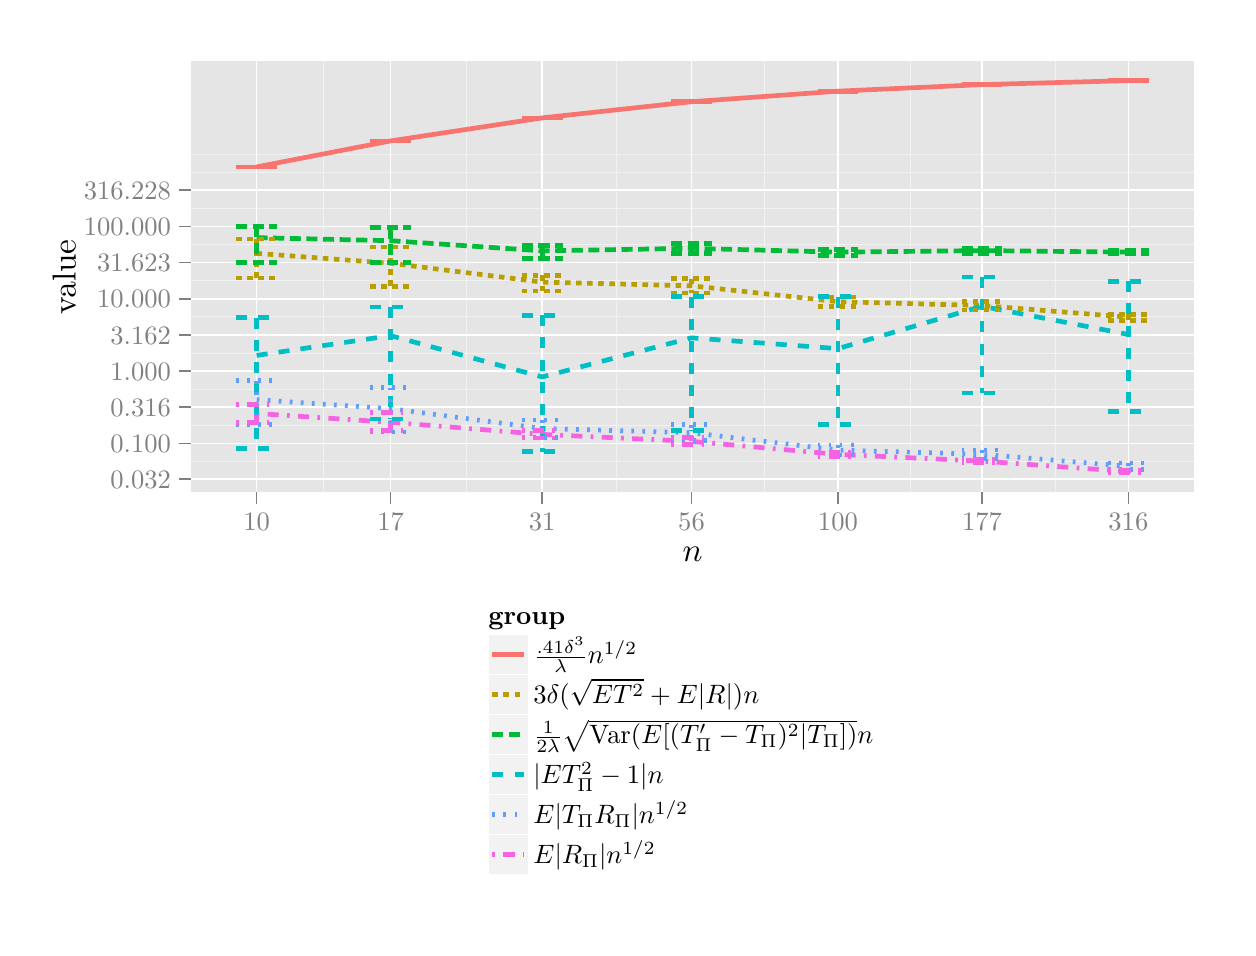
\begin{tikzpicture}[x=1pt,y=1pt]
\definecolor[named]{fillColor}{rgb}{1.00,1.00,1.00}
\path[use as bounding box,fill=fillColor,fill opacity=0.00] (0,0) rectangle (433.62,325.21);
\begin{scope}
\path[clip] (  0.00,  0.00) rectangle (433.62,325.21);
\definecolor[named]{drawColor}{rgb}{1.00,1.00,1.00}
\definecolor[named]{fillColor}{rgb}{1.00,1.00,1.00}

\path[draw=drawColor,line width= 0.6pt,line join=round,line cap=round,fill=fillColor] (  0.00,  0.00) rectangle (433.62,325.21);
\end{scope}
\begin{scope}
\path[clip] ( 58.88,157.27) rectangle (421.57,313.17);
\definecolor[named]{fillColor}{rgb}{0.90,0.90,0.90}

\path[fill=fillColor] ( 58.88,157.27) rectangle (421.57,313.17);
\definecolor[named]{drawColor}{rgb}{0.95,0.95,0.95}

\path[draw=drawColor,line width= 0.3pt,line join=round] ( 58.88,168.50) --
	(421.57,168.50);

\path[draw=drawColor,line width= 0.3pt,line join=round] ( 58.88,181.50) --
	(421.57,181.50);

\path[draw=drawColor,line width= 0.3pt,line join=round] ( 58.88,194.57) --
	(421.57,194.57);

\path[draw=drawColor,line width= 0.3pt,line join=round] ( 58.88,207.64) --
	(421.57,207.64);

\path[draw=drawColor,line width= 0.3pt,line join=round] ( 58.88,220.71) --
	(421.57,220.71);

\path[draw=drawColor,line width= 0.3pt,line join=round] ( 58.88,233.78) --
	(421.57,233.78);

\path[draw=drawColor,line width= 0.3pt,line join=round] ( 58.88,246.85) --
	(421.57,246.85);

\path[draw=drawColor,line width= 0.3pt,line join=round] ( 58.88,259.92) --
	(421.57,259.92);

\path[draw=drawColor,line width= 0.3pt,line join=round] ( 58.88,272.93) --
	(421.57,272.93);

\path[draw=drawColor,line width= 0.3pt,line join=round] ( 58.88,279.39) --
	(421.57,279.39);

\path[draw=drawColor,line width= 0.3pt,line join=round] (106.92,157.27) --
	(106.92,313.17);

\path[draw=drawColor,line width= 0.3pt,line join=round] (158.53,157.27) --
	(158.53,313.17);

\path[draw=drawColor,line width= 0.3pt,line join=round] (212.91,157.27) --
	(212.91,313.17);

\path[draw=drawColor,line width= 0.3pt,line join=round] (266.33,157.27) --
	(266.33,313.17);

\path[draw=drawColor,line width= 0.3pt,line join=round] (318.82,157.27) --
	(318.82,313.17);

\path[draw=drawColor,line width= 0.3pt,line join=round] (371.30,157.27) --
	(371.30,313.17);
\definecolor[named]{drawColor}{rgb}{1.00,1.00,1.00}

\path[draw=drawColor,line width= 0.6pt,line join=round] ( 58.88,162.03) --
	(421.57,162.03);

\path[draw=drawColor,line width= 0.6pt,line join=round] ( 58.88,174.97) --
	(421.57,174.97);

\path[draw=drawColor,line width= 0.6pt,line join=round] ( 58.88,188.03) --
	(421.57,188.03);

\path[draw=drawColor,line width= 0.6pt,line join=round] ( 58.88,201.11) --
	(421.57,201.11);

\path[draw=drawColor,line width= 0.6pt,line join=round] ( 58.88,214.18) --
	(421.57,214.18);

\path[draw=drawColor,line width= 0.6pt,line join=round] ( 58.88,227.25) --
	(421.57,227.25);

\path[draw=drawColor,line width= 0.6pt,line join=round] ( 58.88,240.32) --
	(421.57,240.32);

\path[draw=drawColor,line width= 0.6pt,line join=round] ( 58.88,253.39) --
	(421.57,253.39);

\path[draw=drawColor,line width= 0.6pt,line join=round] ( 58.88,266.46) --
	(421.57,266.46);

\path[draw=drawColor,line width= 0.6pt,line join=round] ( 82.72,157.27) --
	( 82.72,313.17);

\path[draw=drawColor,line width= 0.6pt,line join=round] (131.13,157.27) --
	(131.13,313.17);

\path[draw=drawColor,line width= 0.6pt,line join=round] (185.93,157.27) --
	(185.93,313.17);

\path[draw=drawColor,line width= 0.6pt,line join=round] (239.88,157.27) --
	(239.88,313.17);

\path[draw=drawColor,line width= 0.6pt,line join=round] (292.78,157.27) --
	(292.78,313.17);

\path[draw=drawColor,line width= 0.6pt,line join=round] (344.86,157.27) --
	(344.86,313.17);

\path[draw=drawColor,line width= 0.6pt,line join=round] (397.74,157.27) --
	(397.74,313.17);
\definecolor[named]{drawColor}{rgb}{0.97,0.46,0.43}

\path[draw=drawColor,line width= 1.7pt,line join=round] ( 82.72,274.89) --
	(131.13,284.28) --
	(185.93,292.61) --
	(239.88,298.45) --
	(292.78,302.26) --
	(344.86,304.63) --
	(397.74,306.08);
\definecolor[named]{drawColor}{rgb}{0.72,0.62,0.00}

\path[draw=drawColor,line width= 1.7pt,dash pattern=on 2pt off 2pt ,line join=round] ( 82.72,243.66) --
	(131.13,240.08) --
	(185.93,233.27) --
	(239.88,231.93) --
	(292.78,226.20) --
	(344.86,224.80) --
	(397.74,220.60);
\definecolor[named]{drawColor}{rgb}{0.00,0.73,0.22}

\path[draw=drawColor,line width= 1.7pt,dash pattern=on 4pt off 2pt ,line join=round] ( 82.72,249.33) --
	(131.13,248.23) --
	(185.93,244.56) --
	(239.88,245.48) --
	(292.78,244.09) --
	(344.86,244.65) --
	(397.74,244.10);
\definecolor[named]{drawColor}{rgb}{0.00,0.75,0.77}

\path[draw=drawColor,line width= 1.7pt,dash pattern=on 4pt off 4pt ,line join=round] ( 82.72,206.77) --
	(131.13,213.92) --
	(185.93,199.00) --
	(239.88,213.13) --
	(292.78,209.23) --
	(344.86,224.54) --
	(397.74,214.35);
\definecolor[named]{drawColor}{rgb}{0.38,0.61,1.00}

\path[draw=drawColor,line width= 1.7pt,dash pattern=on 1pt off 3pt ,line join=round] ( 82.72,190.78) --
	(131.13,187.54) --
	(185.93,180.37) --
	(239.88,178.84) --
	(292.78,172.56) --
	(344.86,171.06) --
	(397.74,166.69);
\definecolor[named]{drawColor}{rgb}{0.96,0.39,0.89}

\path[draw=drawColor,line width= 1.7pt,dash pattern=on 1pt off 3pt on 4pt off 3pt ,line join=round] ( 82.72,185.80) --
	(131.13,182.62) --
	(185.93,178.24) --
	(239.88,175.72) --
	(292.78,171.01) --
	(344.86,168.59) --
	(397.74,164.80);
\definecolor[named]{drawColor}{rgb}{0.97,0.46,0.43}

\path[draw=drawColor,line width= 1.7pt,line join=round] ( 75.37,274.89) --
	( 90.07,274.89);

\path[draw=drawColor,line width= 1.7pt,line join=round] ( 82.72,274.89) --
	( 82.72,274.89);

\path[draw=drawColor,line width= 1.7pt,line join=round] ( 75.37,274.89) --
	( 90.07,274.89);

\path[draw=drawColor,line width= 1.7pt,line join=round] (123.78,284.28) --
	(138.48,284.28);

\path[draw=drawColor,line width= 1.7pt,line join=round] (131.13,284.28) --
	(131.13,284.28);

\path[draw=drawColor,line width= 1.7pt,line join=round] (123.78,284.28) --
	(138.48,284.28);

\path[draw=drawColor,line width= 1.7pt,line join=round] (178.58,292.61) --
	(193.28,292.61);

\path[draw=drawColor,line width= 1.7pt,line join=round] (185.93,292.61) --
	(185.93,292.61);

\path[draw=drawColor,line width= 1.7pt,line join=round] (178.58,292.61) --
	(193.28,292.61);

\path[draw=drawColor,line width= 1.7pt,line join=round] (232.53,298.45) --
	(247.23,298.45);

\path[draw=drawColor,line width= 1.7pt,line join=round] (239.88,298.45) --
	(239.88,298.45);

\path[draw=drawColor,line width= 1.7pt,line join=round] (232.53,298.45) --
	(247.23,298.45);

\path[draw=drawColor,line width= 1.7pt,line join=round] (285.42,302.26) --
	(300.13,302.26);

\path[draw=drawColor,line width= 1.7pt,line join=round] (292.78,302.26) --
	(292.78,302.26);

\path[draw=drawColor,line width= 1.7pt,line join=round] (285.42,302.26) --
	(300.13,302.26);

\path[draw=drawColor,line width= 1.7pt,line join=round] (337.51,304.63) --
	(352.22,304.63);

\path[draw=drawColor,line width= 1.7pt,line join=round] (344.86,304.63) --
	(344.86,304.63);

\path[draw=drawColor,line width= 1.7pt,line join=round] (337.51,304.63) --
	(352.22,304.63);

\path[draw=drawColor,line width= 1.7pt,line join=round] (390.39,306.08) --
	(405.09,306.08);

\path[draw=drawColor,line width= 1.7pt,line join=round] (397.74,306.08) --
	(397.74,306.08);

\path[draw=drawColor,line width= 1.7pt,line join=round] (390.39,306.08) --
	(405.09,306.08);
\definecolor[named]{drawColor}{rgb}{0.72,0.62,0.00}

\path[draw=drawColor,line width= 1.7pt,dash pattern=on 2pt off 2pt ,line join=round] ( 75.37,248.87) --
	( 90.07,248.87);

\path[draw=drawColor,line width= 1.7pt,dash pattern=on 2pt off 2pt ,line join=round] ( 82.72,248.87) --
	( 82.72,234.74);

\path[draw=drawColor,line width= 1.7pt,dash pattern=on 2pt off 2pt ,line join=round] ( 75.37,234.74) --
	( 90.07,234.74);

\path[draw=drawColor,line width= 1.7pt,dash pattern=on 2pt off 2pt ,line join=round] (123.78,245.97) --
	(138.48,245.97);

\path[draw=drawColor,line width= 1.7pt,dash pattern=on 2pt off 2pt ,line join=round] (131.13,245.97) --
	(131.13,231.80);

\path[draw=drawColor,line width= 1.7pt,dash pattern=on 2pt off 2pt ,line join=round] (123.78,231.80) --
	(138.48,231.80);

\path[draw=drawColor,line width= 1.7pt,dash pattern=on 2pt off 2pt ,line join=round] (178.58,235.77) --
	(193.28,235.77);

\path[draw=drawColor,line width= 1.7pt,dash pattern=on 2pt off 2pt ,line join=round] (185.93,235.77) --
	(185.93,230.09);

\path[draw=drawColor,line width= 1.7pt,dash pattern=on 2pt off 2pt ,line join=round] (178.58,230.09) --
	(193.28,230.09);

\path[draw=drawColor,line width= 1.7pt,dash pattern=on 2pt off 2pt ,line join=round] (232.53,234.49) --
	(247.23,234.49);

\path[draw=drawColor,line width= 1.7pt,dash pattern=on 2pt off 2pt ,line join=round] (239.88,234.49) --
	(239.88,229.34);

\path[draw=drawColor,line width= 1.7pt,dash pattern=on 2pt off 2pt ,line join=round] (232.53,229.34) --
	(247.23,229.34);

\path[draw=drawColor,line width= 1.7pt,dash pattern=on 2pt off 2pt ,line join=round] (285.42,227.86) --
	(300.13,227.86);

\path[draw=drawColor,line width= 1.7pt,dash pattern=on 2pt off 2pt ,line join=round] (292.78,227.86) --
	(292.78,224.41);

\path[draw=drawColor,line width= 1.7pt,dash pattern=on 2pt off 2pt ,line join=round] (285.42,224.41) --
	(300.13,224.41);

\path[draw=drawColor,line width= 1.7pt,dash pattern=on 2pt off 2pt ,line join=round] (337.51,226.29) --
	(352.22,226.29);

\path[draw=drawColor,line width= 1.7pt,dash pattern=on 2pt off 2pt ,line join=round] (344.86,226.29) --
	(344.86,223.23);

\path[draw=drawColor,line width= 1.7pt,dash pattern=on 2pt off 2pt ,line join=round] (337.51,223.23) --
	(352.22,223.23);

\path[draw=drawColor,line width= 1.7pt,dash pattern=on 2pt off 2pt ,line join=round] (390.39,221.68) --
	(405.09,221.68);

\path[draw=drawColor,line width= 1.7pt,dash pattern=on 2pt off 2pt ,line join=round] (397.74,221.68) --
	(397.74,219.48);

\path[draw=drawColor,line width= 1.7pt,dash pattern=on 2pt off 2pt ,line join=round] (390.39,219.48) --
	(405.09,219.48);
\definecolor[named]{drawColor}{rgb}{0.00,0.73,0.22}

\path[draw=drawColor,line width= 1.7pt,dash pattern=on 4pt off 2pt ,line join=round] ( 75.37,253.42) --
	( 90.07,253.42);

\path[draw=drawColor,line width= 1.7pt,dash pattern=on 4pt off 2pt ,line join=round] ( 82.72,253.42) --
	( 82.72,240.31);

\path[draw=drawColor,line width= 1.7pt,dash pattern=on 4pt off 2pt ,line join=round] ( 75.37,240.31) --
	( 90.07,240.31);

\path[draw=drawColor,line width= 1.7pt,dash pattern=on 4pt off 2pt ,line join=round] (123.78,252.95) --
	(138.48,252.95);

\path[draw=drawColor,line width= 1.7pt,dash pattern=on 4pt off 2pt ,line join=round] (131.13,252.95) --
	(131.13,240.33);

\path[draw=drawColor,line width= 1.7pt,dash pattern=on 4pt off 2pt ,line join=round] (123.78,240.33) --
	(138.48,240.33);

\path[draw=drawColor,line width= 1.7pt,dash pattern=on 4pt off 2pt ,line join=round] (178.58,246.46) --
	(193.28,246.46);

\path[draw=drawColor,line width= 1.7pt,dash pattern=on 4pt off 2pt ,line join=round] (185.93,246.46) --
	(185.93,241.88);

\path[draw=drawColor,line width= 1.7pt,dash pattern=on 4pt off 2pt ,line join=round] (178.58,241.88) --
	(193.28,241.88);

\path[draw=drawColor,line width= 1.7pt,dash pattern=on 4pt off 2pt ,line join=round] (232.53,247.11) --
	(247.23,247.11);

\path[draw=drawColor,line width= 1.7pt,dash pattern=on 4pt off 2pt ,line join=round] (239.88,247.11) --
	(239.88,243.71);

\path[draw=drawColor,line width= 1.7pt,dash pattern=on 4pt off 2pt ,line join=round] (232.53,243.71) --
	(247.23,243.71);

\path[draw=drawColor,line width= 1.7pt,dash pattern=on 4pt off 2pt ,line join=round] (285.42,245.16) --
	(300.13,245.16);

\path[draw=drawColor,line width= 1.7pt,dash pattern=on 4pt off 2pt ,line join=round] (292.78,245.16) --
	(292.78,242.89);

\path[draw=drawColor,line width= 1.7pt,dash pattern=on 4pt off 2pt ,line join=round] (285.42,242.89) --
	(300.13,242.89);

\path[draw=drawColor,line width= 1.7pt,dash pattern=on 4pt off 2pt ,line join=round] (337.51,245.53) --
	(352.22,245.53);

\path[draw=drawColor,line width= 1.7pt,dash pattern=on 4pt off 2pt ,line join=round] (344.86,245.53) --
	(344.86,243.65);

\path[draw=drawColor,line width= 1.7pt,dash pattern=on 4pt off 2pt ,line join=round] (337.51,243.65) --
	(352.22,243.65);

\path[draw=drawColor,line width= 1.7pt,dash pattern=on 4pt off 2pt ,line join=round] (390.39,244.74) --
	(405.09,244.74);

\path[draw=drawColor,line width= 1.7pt,dash pattern=on 4pt off 2pt ,line join=round] (397.74,244.74) --
	(397.74,243.44);

\path[draw=drawColor,line width= 1.7pt,dash pattern=on 4pt off 2pt ,line join=round] (390.39,243.44) --
	(405.09,243.44);
\definecolor[named]{drawColor}{rgb}{0.00,0.75,0.77}

\path[draw=drawColor,line width= 1.7pt,dash pattern=on 4pt off 4pt ,line join=round] ( 75.37,220.42) --
	( 90.07,220.42);

\path[draw=drawColor,line width= 1.7pt,dash pattern=on 4pt off 4pt ,line join=round] ( 82.72,220.42) --
	( 82.72,173.09);

\path[draw=drawColor,line width= 1.7pt,dash pattern=on 4pt off 4pt ,line join=round] ( 75.37,173.09) --
	( 90.07,173.09);

\path[draw=drawColor,line width= 1.7pt,dash pattern=on 4pt off 4pt ,line join=round] (123.78,224.22) --
	(138.48,224.22);

\path[draw=drawColor,line width= 1.7pt,dash pattern=on 4pt off 4pt ,line join=round] (131.13,224.22) --
	(131.13,183.80);

\path[draw=drawColor,line width= 1.7pt,dash pattern=on 4pt off 4pt ,line join=round] (123.78,183.80) --
	(138.48,183.80);

\path[draw=drawColor,line width= 1.7pt,dash pattern=on 4pt off 4pt ,line join=round] (178.58,221.29) --
	(193.28,221.29);

\path[draw=drawColor,line width= 1.7pt,dash pattern=on 4pt off 4pt ,line join=round] (185.93,221.29) --
	(185.93,172.02);

\path[draw=drawColor,line width= 1.7pt,dash pattern=on 4pt off 4pt ,line join=round] (178.58,172.02) --
	(193.28,172.02);

\path[draw=drawColor,line width= 1.7pt,dash pattern=on 4pt off 4pt ,line join=round] (232.53,228.00) --
	(247.23,228.00);

\path[draw=drawColor,line width= 1.7pt,dash pattern=on 4pt off 4pt ,line join=round] (239.88,228.00) --
	(239.88,179.75);

\path[draw=drawColor,line width= 1.7pt,dash pattern=on 4pt off 4pt ,line join=round] (232.53,179.75) --
	(247.23,179.75);

\path[draw=drawColor,line width= 1.7pt,dash pattern=on 4pt off 4pt ,line join=round] (285.42,228.02) --
	(300.13,228.02);

\path[draw=drawColor,line width= 1.7pt,dash pattern=on 4pt off 4pt ,line join=round] (292.78,228.02) --
	(292.78,181.91);

\path[draw=drawColor,line width= 1.7pt,dash pattern=on 4pt off 4pt ,line join=round] (285.42,181.91) --
	(300.13,181.91);

\path[draw=drawColor,line width= 1.7pt,dash pattern=on 4pt off 4pt ,line join=round] (337.51,235.07) --
	(352.22,235.07);

\path[draw=drawColor,line width= 1.7pt,dash pattern=on 4pt off 4pt ,line join=round] (344.86,235.07) --
	(344.86,193.17);

\path[draw=drawColor,line width= 1.7pt,dash pattern=on 4pt off 4pt ,line join=round] (337.51,193.17) --
	(352.22,193.17);

\path[draw=drawColor,line width= 1.7pt,dash pattern=on 4pt off 4pt ,line join=round] (390.39,233.58) --
	(405.09,233.58);

\path[draw=drawColor,line width= 1.7pt,dash pattern=on 4pt off 4pt ,line join=round] (397.74,233.58) --
	(397.74,186.61);

\path[draw=drawColor,line width= 1.7pt,dash pattern=on 4pt off 4pt ,line join=round] (390.39,186.61) --
	(405.09,186.61);
\definecolor[named]{drawColor}{rgb}{0.38,0.61,1.00}

\path[draw=drawColor,line width= 1.7pt,dash pattern=on 1pt off 3pt ,line join=round] ( 75.37,197.61) --
	( 90.07,197.61);

\path[draw=drawColor,line width= 1.7pt,dash pattern=on 1pt off 3pt ,line join=round] ( 82.72,197.61) --
	( 82.72,181.75);

\path[draw=drawColor,line width= 1.7pt,dash pattern=on 1pt off 3pt ,line join=round] ( 75.37,181.75) --
	( 90.07,181.75);

\path[draw=drawColor,line width= 1.7pt,dash pattern=on 1pt off 3pt ,line join=round] (123.78,195.10) --
	(138.48,195.10);

\path[draw=drawColor,line width= 1.7pt,dash pattern=on 1pt off 3pt ,line join=round] (131.13,195.10) --
	(131.13,179.14);

\path[draw=drawColor,line width= 1.7pt,dash pattern=on 1pt off 3pt ,line join=round] (123.78,179.14) --
	(138.48,179.14);

\path[draw=drawColor,line width= 1.7pt,dash pattern=on 1pt off 3pt ,line join=round] (178.58,183.39) --
	(193.28,183.39);

\path[draw=drawColor,line width= 1.7pt,dash pattern=on 1pt off 3pt ,line join=round] (185.93,183.39) --
	(185.93,177.06);

\path[draw=drawColor,line width= 1.7pt,dash pattern=on 1pt off 3pt ,line join=round] (178.58,177.06) --
	(193.28,177.06);

\path[draw=drawColor,line width= 1.7pt,dash pattern=on 1pt off 3pt ,line join=round] (232.53,181.72) --
	(247.23,181.72);

\path[draw=drawColor,line width= 1.7pt,dash pattern=on 1pt off 3pt ,line join=round] (239.88,181.72) --
	(239.88,176.01);

\path[draw=drawColor,line width= 1.7pt,dash pattern=on 1pt off 3pt ,line join=round] (232.53,176.01) --
	(247.23,176.01);

\path[draw=drawColor,line width= 1.7pt,dash pattern=on 1pt off 3pt ,line join=round] (285.42,174.38) --
	(300.13,174.38);

\path[draw=drawColor,line width= 1.7pt,dash pattern=on 1pt off 3pt ,line join=round] (292.78,174.38) --
	(292.78,170.76);

\path[draw=drawColor,line width= 1.7pt,dash pattern=on 1pt off 3pt ,line join=round] (285.42,170.76) --
	(300.13,170.76);

\path[draw=drawColor,line width= 1.7pt,dash pattern=on 1pt off 3pt ,line join=round] (337.51,172.65) --
	(352.22,172.65);

\path[draw=drawColor,line width= 1.7pt,dash pattern=on 1pt off 3pt ,line join=round] (344.86,172.65) --
	(344.86,169.46);

\path[draw=drawColor,line width= 1.7pt,dash pattern=on 1pt off 3pt ,line join=round] (337.51,169.46) --
	(352.22,169.46);

\path[draw=drawColor,line width= 1.7pt,dash pattern=on 1pt off 3pt ,line join=round] (390.39,167.90) --
	(405.09,167.90);

\path[draw=drawColor,line width= 1.7pt,dash pattern=on 1pt off 3pt ,line join=round] (397.74,167.90) --
	(397.74,165.53);

\path[draw=drawColor,line width= 1.7pt,dash pattern=on 1pt off 3pt ,line join=round] (390.39,165.53) --
	(405.09,165.53);
\definecolor[named]{drawColor}{rgb}{0.96,0.39,0.89}

\path[draw=drawColor,line width= 1.7pt,dash pattern=on 1pt off 3pt on 4pt off 3pt ,line join=round] ( 75.37,189.04) --
	( 90.07,189.04);

\path[draw=drawColor,line width= 1.7pt,dash pattern=on 1pt off 3pt on 4pt off 3pt ,line join=round] ( 82.72,189.04) --
	( 82.72,182.53);

\path[draw=drawColor,line width= 1.7pt,dash pattern=on 1pt off 3pt on 4pt off 3pt ,line join=round] ( 75.37,182.53) --
	( 90.07,182.53);

\path[draw=drawColor,line width= 1.7pt,dash pattern=on 1pt off 3pt on 4pt off 3pt ,line join=round] (123.78,186.20) --
	(138.48,186.20);

\path[draw=drawColor,line width= 1.7pt,dash pattern=on 1pt off 3pt on 4pt off 3pt ,line join=round] (131.13,186.20) --
	(131.13,179.73);

\path[draw=drawColor,line width= 1.7pt,dash pattern=on 1pt off 3pt on 4pt off 3pt ,line join=round] (123.78,179.73) --
	(138.48,179.73);

\path[draw=drawColor,line width= 1.7pt,dash pattern=on 1pt off 3pt on 4pt off 3pt ,line join=round] (178.58,179.63) --
	(193.28,179.63);

\path[draw=drawColor,line width= 1.7pt,dash pattern=on 1pt off 3pt on 4pt off 3pt ,line join=round] (185.93,179.63) --
	(185.93,176.94);

\path[draw=drawColor,line width= 1.7pt,dash pattern=on 1pt off 3pt on 4pt off 3pt ,line join=round] (178.58,176.94) --
	(193.28,176.94);

\path[draw=drawColor,line width= 1.7pt,dash pattern=on 1pt off 3pt on 4pt off 3pt ,line join=round] (232.53,176.99) --
	(247.23,176.99);

\path[draw=drawColor,line width= 1.7pt,dash pattern=on 1pt off 3pt on 4pt off 3pt ,line join=round] (239.88,176.99) --
	(239.88,174.54);

\path[draw=drawColor,line width= 1.7pt,dash pattern=on 1pt off 3pt on 4pt off 3pt ,line join=round] (232.53,174.54) --
	(247.23,174.54);

\path[draw=drawColor,line width= 1.7pt,dash pattern=on 1pt off 3pt on 4pt off 3pt ,line join=round] (285.42,171.79) --
	(300.13,171.79);

\path[draw=drawColor,line width= 1.7pt,dash pattern=on 1pt off 3pt on 4pt off 3pt ,line join=round] (292.78,171.79) --
	(292.78,170.31);

\path[draw=drawColor,line width= 1.7pt,dash pattern=on 1pt off 3pt on 4pt off 3pt ,line join=round] (285.42,170.31) --
	(300.13,170.31);

\path[draw=drawColor,line width= 1.7pt,dash pattern=on 1pt off 3pt on 4pt off 3pt ,line join=round] (337.51,169.29) --
	(352.22,169.29);

\path[draw=drawColor,line width= 1.7pt,dash pattern=on 1pt off 3pt on 4pt off 3pt ,line join=round] (344.86,169.29) --
	(344.86,167.97);

\path[draw=drawColor,line width= 1.7pt,dash pattern=on 1pt off 3pt on 4pt off 3pt ,line join=round] (337.51,167.97) --
	(352.22,167.97);

\path[draw=drawColor,line width= 1.7pt,dash pattern=on 1pt off 3pt on 4pt off 3pt ,line join=round] (390.39,165.25) --
	(405.09,165.25);

\path[draw=drawColor,line width= 1.7pt,dash pattern=on 1pt off 3pt on 4pt off 3pt ,line join=round] (397.74,165.25) --
	(397.74,164.35);

\path[draw=drawColor,line width= 1.7pt,dash pattern=on 1pt off 3pt on 4pt off 3pt ,line join=round] (390.39,164.35) --
	(405.09,164.35);
\end{scope}
\begin{scope}
\path[clip] (  0.00,  0.00) rectangle (433.62,325.21);
\definecolor[named]{drawColor}{rgb}{0.50,0.50,0.50}

\node[text=drawColor,anchor=base east,inner sep=0pt, outer sep=0pt, scale=  0.96] at ( 51.77,158.73) {0.032};

\node[text=drawColor,anchor=base east,inner sep=0pt, outer sep=0pt, scale=  0.96] at ( 51.77,171.66) {0.100};

\node[text=drawColor,anchor=base east,inner sep=0pt, outer sep=0pt, scale=  0.96] at ( 51.77,184.72) {0.316};

\node[text=drawColor,anchor=base east,inner sep=0pt, outer sep=0pt, scale=  0.96] at ( 51.77,197.80) {1.000};

\node[text=drawColor,anchor=base east,inner sep=0pt, outer sep=0pt, scale=  0.96] at ( 51.77,210.87) {3.162};

\node[text=drawColor,anchor=base east,inner sep=0pt, outer sep=0pt, scale=  0.96] at ( 51.77,223.94) {10.000};

\node[text=drawColor,anchor=base east,inner sep=0pt, outer sep=0pt, scale=  0.96] at ( 51.77,237.01) {31.623};

\node[text=drawColor,anchor=base east,inner sep=0pt, outer sep=0pt, scale=  0.96] at ( 51.77,250.08) {100.000};

\node[text=drawColor,anchor=base east,inner sep=0pt, outer sep=0pt, scale=  0.96] at ( 51.77,263.15) {316.228};
\end{scope}
\begin{scope}
\path[clip] (  0.00,  0.00) rectangle (433.62,325.21);
\definecolor[named]{drawColor}{rgb}{0.50,0.50,0.50}

\path[draw=drawColor,line width= 0.6pt,line join=round] ( 54.61,162.03) --
	( 58.88,162.03);

\path[draw=drawColor,line width= 0.6pt,line join=round] ( 54.61,174.97) --
	( 58.88,174.97);

\path[draw=drawColor,line width= 0.6pt,line join=round] ( 54.61,188.03) --
	( 58.88,188.03);

\path[draw=drawColor,line width= 0.6pt,line join=round] ( 54.61,201.11) --
	( 58.88,201.11);

\path[draw=drawColor,line width= 0.6pt,line join=round] ( 54.61,214.18) --
	( 58.88,214.18);

\path[draw=drawColor,line width= 0.6pt,line join=round] ( 54.61,227.25) --
	( 58.88,227.25);

\path[draw=drawColor,line width= 0.6pt,line join=round] ( 54.61,240.32) --
	( 58.88,240.32);

\path[draw=drawColor,line width= 0.6pt,line join=round] ( 54.61,253.39) --
	( 58.88,253.39);

\path[draw=drawColor,line width= 0.6pt,line join=round] ( 54.61,266.46) --
	( 58.88,266.46);
\end{scope}
\begin{scope}
\path[clip] (  0.00,  0.00) rectangle (433.62,325.21);
\definecolor[named]{drawColor}{rgb}{0.50,0.50,0.50}

\path[draw=drawColor,line width= 0.6pt,line join=round] ( 82.72,153.00) --
	( 82.72,157.27);

\path[draw=drawColor,line width= 0.6pt,line join=round] (131.13,153.00) --
	(131.13,157.27);

\path[draw=drawColor,line width= 0.6pt,line join=round] (185.93,153.00) --
	(185.93,157.27);

\path[draw=drawColor,line width= 0.6pt,line join=round] (239.88,153.00) --
	(239.88,157.27);

\path[draw=drawColor,line width= 0.6pt,line join=round] (292.78,153.00) --
	(292.78,157.27);

\path[draw=drawColor,line width= 0.6pt,line join=round] (344.86,153.00) --
	(344.86,157.27);

\path[draw=drawColor,line width= 0.6pt,line join=round] (397.74,153.00) --
	(397.74,157.27);
\end{scope}
\begin{scope}
\path[clip] (  0.00,  0.00) rectangle (433.62,325.21);
\definecolor[named]{drawColor}{rgb}{0.50,0.50,0.50}

\node[text=drawColor,anchor=base,inner sep=0pt, outer sep=0pt, scale=  0.96] at ( 82.72,143.54) {10};

\node[text=drawColor,anchor=base,inner sep=0pt, outer sep=0pt, scale=  0.96] at (131.13,143.54) {17};

\node[text=drawColor,anchor=base,inner sep=0pt, outer sep=0pt, scale=  0.96] at (185.93,143.54) {31};

\node[text=drawColor,anchor=base,inner sep=0pt, outer sep=0pt, scale=  0.96] at (239.88,143.54) {56};

\node[text=drawColor,anchor=base,inner sep=0pt, outer sep=0pt, scale=  0.96] at (292.78,143.54) {100};

\node[text=drawColor,anchor=base,inner sep=0pt, outer sep=0pt, scale=  0.96] at (344.86,143.54) {177};

\node[text=drawColor,anchor=base,inner sep=0pt, outer sep=0pt, scale=  0.96] at (397.74,143.54) {316};
\end{scope}
\begin{scope}
\path[clip] (  0.00,  0.00) rectangle (433.62,325.21);
\definecolor[named]{drawColor}{rgb}{0.00,0.00,0.00}

\node[text=drawColor,anchor=base,inner sep=0pt, outer sep=0pt, scale=  1.20] at (240.23,132.27) {$n$};
\end{scope}
\begin{scope}
\path[clip] (  0.00,  0.00) rectangle (433.62,325.21);
\definecolor[named]{drawColor}{rgb}{0.00,0.00,0.00}

\node[text=drawColor,rotate= 90.00,anchor=base,inner sep=0pt, outer sep=0pt, scale=  1.20] at ( 17.30,235.22) {value};
\end{scope}
\begin{scope}
\path[clip] (  0.00,  0.00) rectangle (433.62,325.21);
\definecolor[named]{fillColor}{rgb}{1.00,1.00,1.00}

\path[fill=fillColor] (162.21, 14.89) rectangle (318.25,120.39);
\end{scope}
\begin{scope}
\path[clip] (  0.00,  0.00) rectangle (433.62,325.21);
\definecolor[named]{drawColor}{rgb}{0.00,0.00,0.00}

\node[text=drawColor,anchor=base west,inner sep=0pt, outer sep=0pt, scale=  0.96] at (166.47,109.50) {\bfseries group};
\end{scope}
\begin{scope}
\path[clip] (  0.00,  0.00) rectangle (433.62,325.21);
\definecolor[named]{drawColor}{rgb}{1.00,1.00,1.00}
\definecolor[named]{fillColor}{rgb}{0.95,0.95,0.95}

\path[draw=drawColor,line width= 0.6pt,line join=round,line cap=round,fill=fillColor] (166.47, 91.43) rectangle (180.93,105.88);
\end{scope}
\begin{scope}
\path[clip] (  0.00,  0.00) rectangle (433.62,325.21);
\definecolor[named]{drawColor}{rgb}{0.97,0.46,0.43}

\path[draw=drawColor,line width= 1.7pt,line join=round] (167.92, 98.66) -- (179.48, 98.66);
\end{scope}
\begin{scope}
\path[clip] (  0.00,  0.00) rectangle (433.62,325.21);
\definecolor[named]{drawColor}{rgb}{0.97,0.46,0.43}

\path[draw=drawColor,line width= 1.7pt,line join=round] (167.92, 98.66) -- (179.48, 98.66);
\end{scope}
\begin{scope}
\path[clip] (  0.00,  0.00) rectangle (433.62,325.21);
\definecolor[named]{drawColor}{rgb}{1.00,1.00,1.00}
\definecolor[named]{fillColor}{rgb}{0.95,0.95,0.95}

\path[draw=drawColor,line width= 0.6pt,line join=round,line cap=round,fill=fillColor] (166.47, 76.97) rectangle (180.93, 91.43);
\end{scope}
\begin{scope}
\path[clip] (  0.00,  0.00) rectangle (433.62,325.21);
\definecolor[named]{drawColor}{rgb}{0.72,0.62,0.00}

\path[draw=drawColor,line width= 1.7pt,dash pattern=on 2pt off 2pt ,line join=round] (167.92, 84.20) -- (179.48, 84.20);
\end{scope}
\begin{scope}
\path[clip] (  0.00,  0.00) rectangle (433.62,325.21);
\definecolor[named]{drawColor}{rgb}{0.72,0.62,0.00}

\path[draw=drawColor,line width= 1.7pt,dash pattern=on 2pt off 2pt ,line join=round] (167.92, 84.20) -- (179.48, 84.20);
\end{scope}
\begin{scope}
\path[clip] (  0.00,  0.00) rectangle (433.62,325.21);
\definecolor[named]{drawColor}{rgb}{1.00,1.00,1.00}
\definecolor[named]{fillColor}{rgb}{0.95,0.95,0.95}

\path[draw=drawColor,line width= 0.6pt,line join=round,line cap=round,fill=fillColor] (166.47, 62.52) rectangle (180.93, 76.97);
\end{scope}
\begin{scope}
\path[clip] (  0.00,  0.00) rectangle (433.62,325.21);
\definecolor[named]{drawColor}{rgb}{0.00,0.73,0.22}

\path[draw=drawColor,line width= 1.7pt,dash pattern=on 4pt off 2pt ,line join=round] (167.92, 69.75) -- (179.48, 69.75);
\end{scope}
\begin{scope}
\path[clip] (  0.00,  0.00) rectangle (433.62,325.21);
\definecolor[named]{drawColor}{rgb}{0.00,0.73,0.22}

\path[draw=drawColor,line width= 1.7pt,dash pattern=on 4pt off 2pt ,line join=round] (167.92, 69.75) -- (179.48, 69.75);
\end{scope}
\begin{scope}
\path[clip] (  0.00,  0.00) rectangle (433.62,325.21);
\definecolor[named]{drawColor}{rgb}{1.00,1.00,1.00}
\definecolor[named]{fillColor}{rgb}{0.95,0.95,0.95}

\path[draw=drawColor,line width= 0.6pt,line join=round,line cap=round,fill=fillColor] (166.47, 48.07) rectangle (180.93, 62.52);
\end{scope}
\begin{scope}
\path[clip] (  0.00,  0.00) rectangle (433.62,325.21);
\definecolor[named]{drawColor}{rgb}{0.00,0.75,0.77}

\path[draw=drawColor,line width= 1.7pt,dash pattern=on 4pt off 4pt ,line join=round] (167.92, 55.29) -- (179.48, 55.29);
\end{scope}
\begin{scope}
\path[clip] (  0.00,  0.00) rectangle (433.62,325.21);
\definecolor[named]{drawColor}{rgb}{0.00,0.75,0.77}

\path[draw=drawColor,line width= 1.7pt,dash pattern=on 4pt off 4pt ,line join=round] (167.92, 55.29) -- (179.48, 55.29);
\end{scope}
\begin{scope}
\path[clip] (  0.00,  0.00) rectangle (433.62,325.21);
\definecolor[named]{drawColor}{rgb}{1.00,1.00,1.00}
\definecolor[named]{fillColor}{rgb}{0.95,0.95,0.95}

\path[draw=drawColor,line width= 0.6pt,line join=round,line cap=round,fill=fillColor] (166.47, 33.61) rectangle (180.93, 48.07);
\end{scope}
\begin{scope}
\path[clip] (  0.00,  0.00) rectangle (433.62,325.21);
\definecolor[named]{drawColor}{rgb}{0.38,0.61,1.00}

\path[draw=drawColor,line width= 1.7pt,dash pattern=on 1pt off 3pt ,line join=round] (167.92, 40.84) -- (179.48, 40.84);
\end{scope}
\begin{scope}
\path[clip] (  0.00,  0.00) rectangle (433.62,325.21);
\definecolor[named]{drawColor}{rgb}{0.38,0.61,1.00}

\path[draw=drawColor,line width= 1.7pt,dash pattern=on 1pt off 3pt ,line join=round] (167.92, 40.84) -- (179.48, 40.84);
\end{scope}
\begin{scope}
\path[clip] (  0.00,  0.00) rectangle (433.62,325.21);
\definecolor[named]{drawColor}{rgb}{1.00,1.00,1.00}
\definecolor[named]{fillColor}{rgb}{0.95,0.95,0.95}

\path[draw=drawColor,line width= 0.6pt,line join=round,line cap=round,fill=fillColor] (166.47, 19.16) rectangle (180.93, 33.61);
\end{scope}
\begin{scope}
\path[clip] (  0.00,  0.00) rectangle (433.62,325.21);
\definecolor[named]{drawColor}{rgb}{0.96,0.39,0.89}

\path[draw=drawColor,line width= 1.7pt,dash pattern=on 1pt off 3pt on 4pt off 3pt ,line join=round] (167.92, 26.39) -- (179.48, 26.39);
\end{scope}
\begin{scope}
\path[clip] (  0.00,  0.00) rectangle (433.62,325.21);
\definecolor[named]{drawColor}{rgb}{0.96,0.39,0.89}

\path[draw=drawColor,line width= 1.7pt,dash pattern=on 1pt off 3pt on 4pt off 3pt ,line join=round] (167.92, 26.39) -- (179.48, 26.39);
\end{scope}
\begin{scope}
\path[clip] (  0.00,  0.00) rectangle (433.62,325.21);
\definecolor[named]{drawColor}{rgb}{0.00,0.00,0.00}

\node[text=drawColor,anchor=base west,inner sep=0pt, outer sep=0pt, scale=  0.96] at (182.73, 95.35) {$\frac{.41\delta^3}{\lambda}n^{1/2}\quad $};
\end{scope}
\begin{scope}
\path[clip] (  0.00,  0.00) rectangle (433.62,325.21);
\definecolor[named]{drawColor}{rgb}{0.00,0.00,0.00}

\node[text=drawColor,anchor=base west,inner sep=0pt, outer sep=0pt, scale=  0.96] at (182.73, 80.90) {$3\delta(\sqrt{\mathbb{E}T^2}+\mathbb{E}|R|)n\quad $};
\end{scope}
\begin{scope}
\path[clip] (  0.00,  0.00) rectangle (433.62,325.21);
\definecolor[named]{drawColor}{rgb}{0.00,0.00,0.00}

\node[text=drawColor,anchor=base west,inner sep=0pt, outer sep=0pt, scale=  0.96] at (182.73, 66.44) {$\frac{1}{2\lambda}\sqrt{\mathrm{Var}(\mathbb{E}[(T'_{\Pi}-T_{\Pi})^2|T_{\Pi}])}n\quad $};
\end{scope}
\begin{scope}
\path[clip] (  0.00,  0.00) rectangle (433.62,325.21);
\definecolor[named]{drawColor}{rgb}{0.00,0.00,0.00}

\node[text=drawColor,anchor=base west,inner sep=0pt, outer sep=0pt, scale=  0.96] at (182.73, 51.99) {$|\mathbb{E}T_{\Pi}^2-1|n\quad $};
\end{scope}
\begin{scope}
\path[clip] (  0.00,  0.00) rectangle (433.62,325.21);
\definecolor[named]{drawColor}{rgb}{0.00,0.00,0.00}

\node[text=drawColor,anchor=base west,inner sep=0pt, outer sep=0pt, scale=  0.96] at (182.73, 37.53) {$\mathbb{E}|T_{\Pi}R_{\Pi}|n^{1/2}\quad $};
\end{scope}
\begin{scope}
\path[clip] (  0.00,  0.00) rectangle (433.62,325.21);
\definecolor[named]{drawColor}{rgb}{0.00,0.00,0.00}

\node[text=drawColor,anchor=base west,inner sep=0pt, outer sep=0pt, scale=  0.96] at (182.73, 23.08) {$\mathbb{E}|R_{\Pi}|n^{1/2}\quad $};
\end{scope}
\end{tikzpicture}

  \caption{Log-log plot of values for each term in the bound, calculating the conditional
    expectation exactly ($10N$ permutations each).}
\end{figure}

We shall see that $\frac{.41 \delta^3}{\lambda}N^{1/2}$ is bounded in some situations.
\clearpage

Below, we see a plot of $\frac{.41 \delta^3}{\lambda}N^{1/2}$ on $N$
when $u_i = i$.
\begin{figure}[!ht]
  \centering
  % Created by tikzDevice version 0.6.2-92-0ad2792 on 2013-03-05 17:06:53
% !TEX encoding = UTF-8 Unicode
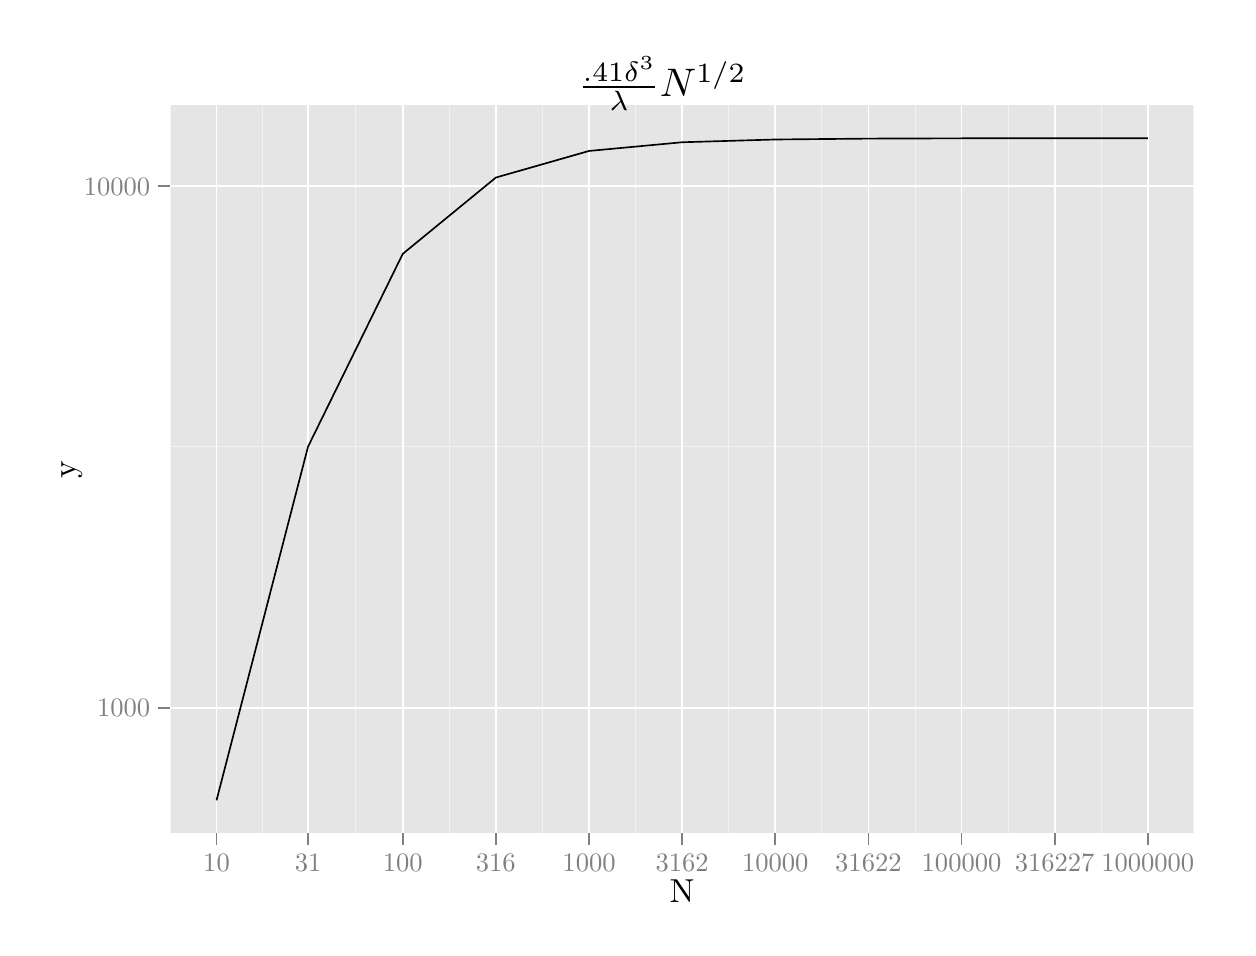
\begin{tikzpicture}[x=1pt,y=1pt]
\definecolor[named]{fillColor}{rgb}{1.00,1.00,1.00}
\path[use as bounding box,fill=fillColor,fill opacity=0.00] (0,0) rectangle (433.62,325.21);
\begin{scope}
\path[clip] (  0.00,  0.00) rectangle (433.62,325.21);
\definecolor[named]{drawColor}{rgb}{1.00,1.00,1.00}
\definecolor[named]{fillColor}{rgb}{1.00,1.00,1.00}

\path[draw=drawColor,line width= 0.6pt,line join=round,line cap=round,fill=fillColor] (  0.00,  0.00) rectangle (433.62,325.21);
\end{scope}
\begin{scope}
\path[clip] ( 51.42, 34.03) rectangle (421.57,297.23);
\definecolor[named]{fillColor}{rgb}{0.90,0.90,0.90}

\path[fill=fillColor] ( 51.42, 34.03) rectangle (421.57,297.23);
\definecolor[named]{drawColor}{rgb}{0.95,0.95,0.95}

\path[draw=drawColor,line width= 0.3pt,line join=round] ( 51.42,173.75) --
	(421.57,173.75);

\path[draw=drawColor,line width= 0.3pt,line join=round] ( 51.71, 34.03) --
	( 51.71,297.23);

\path[draw=drawColor,line width= 0.3pt,line join=round] ( 84.78, 34.03) --
	( 84.78,297.23);

\path[draw=drawColor,line width= 0.3pt,line join=round] (118.43, 34.03) --
	(118.43,297.23);

\path[draw=drawColor,line width= 0.3pt,line join=round] (152.36, 34.03) --
	(152.36,297.23);

\path[draw=drawColor,line width= 0.3pt,line join=round] (186.01, 34.03) --
	(186.01,297.23);

\path[draw=drawColor,line width= 0.3pt,line join=round] (219.67, 34.03) --
	(219.67,297.23);

\path[draw=drawColor,line width= 0.3pt,line join=round] (253.32, 34.03) --
	(253.32,297.23);

\path[draw=drawColor,line width= 0.3pt,line join=round] (286.97, 34.03) --
	(286.97,297.23);

\path[draw=drawColor,line width= 0.3pt,line join=round] (320.62, 34.03) --
	(320.62,297.23);

\path[draw=drawColor,line width= 0.3pt,line join=round] (354.27, 34.03) --
	(354.27,297.23);

\path[draw=drawColor,line width= 0.3pt,line join=round] (387.92, 34.03) --
	(387.92,297.23);

\path[draw=drawColor,line width= 0.3pt,line join=round] (421.28, 34.03) --
	(421.28,297.23);
\definecolor[named]{drawColor}{rgb}{1.00,1.00,1.00}

\path[draw=drawColor,line width= 0.6pt,line join=round] ( 51.42, 79.45) --
	(421.57, 79.45);

\path[draw=drawColor,line width= 0.6pt,line join=round] ( 51.42,268.04) --
	(421.57,268.04);

\path[draw=drawColor,line width= 0.6pt,line join=round] ( 68.24, 34.03) --
	( 68.24,297.23);

\path[draw=drawColor,line width= 0.6pt,line join=round] (101.31, 34.03) --
	(101.31,297.23);

\path[draw=drawColor,line width= 0.6pt,line join=round] (135.54, 34.03) --
	(135.54,297.23);

\path[draw=drawColor,line width= 0.6pt,line join=round] (169.17, 34.03) --
	(169.17,297.23);

\path[draw=drawColor,line width= 0.6pt,line join=round] (202.85, 34.03) --
	(202.85,297.23);

\path[draw=drawColor,line width= 0.6pt,line join=round] (236.49, 34.03) --
	(236.49,297.23);

\path[draw=drawColor,line width= 0.6pt,line join=round] (270.15, 34.03) --
	(270.15,297.23);

\path[draw=drawColor,line width= 0.6pt,line join=round] (303.80, 34.03) --
	(303.80,297.23);

\path[draw=drawColor,line width= 0.6pt,line join=round] (337.45, 34.03) --
	(337.45,297.23);

\path[draw=drawColor,line width= 0.6pt,line join=round] (371.10, 34.03) --
	(371.10,297.23);

\path[draw=drawColor,line width= 0.6pt,line join=round] (404.75, 34.03) --
	(404.75,297.23);
\definecolor[named]{drawColor}{rgb}{0.00,0.00,0.00}

\path[draw=drawColor,line width= 0.6pt,line join=round] ( 68.24, 46.00) --
	(101.31,173.81) --
	(135.54,243.48) --
	(169.17,271.04) --
	(202.85,280.66) --
	(236.49,283.80) --
	(270.15,284.80) --
	(303.80,285.12) --
	(337.45,285.22) --
	(371.10,285.26) --
	(404.75,285.27);
\end{scope}
\begin{scope}
\path[clip] (  0.00,  0.00) rectangle (433.62,325.21);
\definecolor[named]{drawColor}{rgb}{0.50,0.50,0.50}

\node[text=drawColor,anchor=base east,inner sep=0pt, outer sep=0pt, scale=  0.96] at ( 44.30, 76.15) {1000};

\node[text=drawColor,anchor=base east,inner sep=0pt, outer sep=0pt, scale=  0.96] at ( 44.30,264.74) {10000};
\end{scope}
\begin{scope}
\path[clip] (  0.00,  0.00) rectangle (433.62,325.21);
\definecolor[named]{drawColor}{rgb}{0.50,0.50,0.50}

\path[draw=drawColor,line width= 0.6pt,line join=round] ( 47.15, 79.45) --
	( 51.42, 79.45);

\path[draw=drawColor,line width= 0.6pt,line join=round] ( 47.15,268.04) --
	( 51.42,268.04);
\end{scope}
\begin{scope}
\path[clip] (  0.00,  0.00) rectangle (433.62,325.21);
\definecolor[named]{drawColor}{rgb}{0.50,0.50,0.50}

\path[draw=drawColor,line width= 0.6pt,line join=round] ( 68.24, 29.77) --
	( 68.24, 34.03);

\path[draw=drawColor,line width= 0.6pt,line join=round] (101.31, 29.77) --
	(101.31, 34.03);

\path[draw=drawColor,line width= 0.6pt,line join=round] (135.54, 29.77) --
	(135.54, 34.03);

\path[draw=drawColor,line width= 0.6pt,line join=round] (169.17, 29.77) --
	(169.17, 34.03);

\path[draw=drawColor,line width= 0.6pt,line join=round] (202.85, 29.77) --
	(202.85, 34.03);

\path[draw=drawColor,line width= 0.6pt,line join=round] (236.49, 29.77) --
	(236.49, 34.03);

\path[draw=drawColor,line width= 0.6pt,line join=round] (270.15, 29.77) --
	(270.15, 34.03);

\path[draw=drawColor,line width= 0.6pt,line join=round] (303.80, 29.77) --
	(303.80, 34.03);

\path[draw=drawColor,line width= 0.6pt,line join=round] (337.45, 29.77) --
	(337.45, 34.03);

\path[draw=drawColor,line width= 0.6pt,line join=round] (371.10, 29.77) --
	(371.10, 34.03);

\path[draw=drawColor,line width= 0.6pt,line join=round] (404.75, 29.77) --
	(404.75, 34.03);
\end{scope}
\begin{scope}
\path[clip] (  0.00,  0.00) rectangle (433.62,325.21);
\definecolor[named]{drawColor}{rgb}{0.50,0.50,0.50}

\node[text=drawColor,anchor=base,inner sep=0pt, outer sep=0pt, scale=  0.96] at ( 68.24, 20.31) {10};

\node[text=drawColor,anchor=base,inner sep=0pt, outer sep=0pt, scale=  0.96] at (101.31, 20.31) {31};

\node[text=drawColor,anchor=base,inner sep=0pt, outer sep=0pt, scale=  0.96] at (135.54, 20.31) {100};

\node[text=drawColor,anchor=base,inner sep=0pt, outer sep=0pt, scale=  0.96] at (169.17, 20.31) {316};

\node[text=drawColor,anchor=base,inner sep=0pt, outer sep=0pt, scale=  0.96] at (202.85, 20.31) {1000};

\node[text=drawColor,anchor=base,inner sep=0pt, outer sep=0pt, scale=  0.96] at (236.49, 20.31) {3162};

\node[text=drawColor,anchor=base,inner sep=0pt, outer sep=0pt, scale=  0.96] at (270.15, 20.31) {10000};

\node[text=drawColor,anchor=base,inner sep=0pt, outer sep=0pt, scale=  0.96] at (303.80, 20.31) {31622};

\node[text=drawColor,anchor=base,inner sep=0pt, outer sep=0pt, scale=  0.96] at (337.45, 20.31) {100000};

\node[text=drawColor,anchor=base,inner sep=0pt, outer sep=0pt, scale=  0.96] at (371.10, 20.31) {316227};

\node[text=drawColor,anchor=base,inner sep=0pt, outer sep=0pt, scale=  0.96] at (404.75, 20.31) {1000000};
\end{scope}
\begin{scope}
\path[clip] (  0.00,  0.00) rectangle (433.62,325.21);
\definecolor[named]{drawColor}{rgb}{0.00,0.00,0.00}

\node[text=drawColor,anchor=base,inner sep=0pt, outer sep=0pt, scale=  1.20] at (236.50,  9.03) {N};
\end{scope}
\begin{scope}
\path[clip] (  0.00,  0.00) rectangle (433.62,325.21);
\definecolor[named]{drawColor}{rgb}{0.00,0.00,0.00}

\node[text=drawColor,rotate= 90.00,anchor=base,inner sep=0pt, outer sep=0pt, scale=  1.20] at ( 17.30,165.63) {y};
\end{scope}
\begin{scope}
\path[clip] (  0.00,  0.00) rectangle (433.62,325.21);
\definecolor[named]{drawColor}{rgb}{0.00,0.00,0.00}

\node[text=drawColor,anchor=base,inner sep=0pt, outer sep=0pt, scale=  1.44] at (236.50,300.24) {$\frac{.41\delta^3}{\lambda}N^{1/2}\quad $};
\end{scope}
\end{tikzpicture}

  \caption{$\frac{.41 \delta^3}{\lambda}N^{1/2}$ on $N$.}
\end{figure}

Recall that
\begin{equation*}
  \lim_{n \to \infty} \delta \sqrt{n} = 16 \sqrt{6}.
\end{equation*}

\section{Efficient Updates}
\label{S:efficient-updates}
Instead of conditioning on the value of $T_{\Pi}$, we condition on the
observed permutation $\pi$.  For $N$ observations in each group, there
are $N^2 \: T_{\Pi}'$ values that come from swapping one value in the first
group with one value in the second.  $T_{\Pi}'$ should not differ much from
$T_{\Pi}$, and calculating the $t$-statistics from scratch is inefficient.

We use an efficient $t$-statistic update rule to easily calculate
millions of $t$-statistics.  The two sample $t$-statistic is given by
\begin{equation*}
  T_{\Pi} = \frac{\bar{x}-\bar{u}}
  {\sqrt{\frac{2}{n}}\sqrt{\frac{1}{2}(S_X^2+S_U^2)}},
\end{equation*}
where $S_X^2=\frac{1}{N-1}(\sum_{i=1}^Nx_i^2-n\bar{x}^2)$.

Let $T_{x_i,u_j}$ be the result of $T'$ by swapping $x_i$ with $u_j$:
\begin{align*}
  \Delta &\equiv u_j-x_i \\
  \bar{x}_{x_i,u_j} &= \bar{x}-\frac{1}{N}x_i+\frac{1}{N}u_j =
  \bar{x}+\frac{\Delta}{N} \\
  \bar{u}_{x_i,u_j} &= \bar{u}+\frac{1}{N}x_i-\frac{1}{N}u_j =
  \bar{u}-\frac{\Delta}{N} \\
  S_{X_{x_i,u_j}}^2 &= \frac{1}{N-1}(\sum_{k=1}^N x_k^2 - x_i^2 +
  u_j^2) - \frac{N}{N-1}\bar{x}^2_{x_i,u_j} \\
  S_{U_{x_i,u_j}}^2 &= \frac{1}{N-1}(\sum_{k=1}^N u_k^2 + x_i^2 -
  u_j^2) - \frac{N}{N-1}\bar{u}^2_{x_i,u_j} \\
  \bar{x}_{x_i,u_j}^2 &= \bar{x}^2 + \frac{2\Delta}{N}\bar{x} +
  \frac{\Delta^2}{N} \\
  \bar{u}_{x_i,u_j}^2 &= \bar{u}^2 - \frac{2\Delta}{N}\bar{u} + \frac{\Delta^2}{N}
\end{align*}

Then
\begin{align*}
  T_{x_i,u_j} &= \frac{\bar{x}_{x_i,u_j}-\bar{u}_{x_i,u_j}}
  {\sqrt{\frac{2}{N}}\sqrt{\frac{1}{2}(S_{X_{x_i,u_j}}^2+S_{U_{x_i,u_j}}^2)}}\\
  &= \frac{\bar{x}-\bar{u}+\frac{2\Delta}{N}}
  {\sqrt{\frac{2}{N}}\sqrt{\frac{1}{2(N-1)}[\sum_{k=1}^N (x_k^2+u_k^2)
      -N(\bar{x}^2+\bar{u}^2+\Delta(\frac{2\bar{x}}{n}
      -\frac{2\bar{u}}{n})+\frac{2}{n^2}\Delta^2)]}}.
\end{align*}
Only the terms involving $\Delta$ need to be recomputed for each of the $N^2$ swaps.
